\documentclass[letterpaper,10pt]{book}
% Change to 10 pt
\usepackage{pdfpages}
\usepackage{morewrites}			% to counteract the no write space problem
\setcounter{tocdepth}{6}

\usepackage[framemethod=TikZ]{mdframed}

\usepackage{fancyhdr}

\usepackage{paralist}
\usepackage{amsmath}
\usepackage{amsfonts}
\usepackage{amssymb}
\usepackage{graphicx}

\usepackage{datetime}
%\usepackage{ulem}

%\usepackage[nottoc]{toobibind}

\usepackage[inline]{enumitem}

% Outer margin at 2.50 is exacty correct to fit the ``corruption alert'' tables
\usepackage[inner=1.0in, outer=2.50in, top=2.54cm,bottom=2.54cm, marginparwidth=2.25in]{geometry}

\usepackage{marginnote}
\usepackage{longtable}
\usepackage{booktabs}
\usepackage{xcolor}

\usepackage{soul}

%%%%%%%%%%%%
\definecolor{ForestGreen}{rgb}{0.00,0.29,0.098}
%%%%%%%%%%%%

\usepackage{marginnote}

\usepackage{imakeidx} 
\usepackage[
	backref=true,
	style=numeric,
%	citestyle=numeric,
	backend=bibtex
	]{biblatex}
\usepackage[driverfallback=hypertex,colorlinks=True]{hyperref}
\usepackage{cleveref}

\makeindex[name=scripture,columnsep=20pt, columnseprule=True,columns=3, title=Scripture References]
\makeindex[name=speaker,columnsep=20pt, columnseprule=True,,columns=2, title=Sermon Creator]
\makeindex[name=series,columnsep=20pt, columnseprule=True,,columns=2, title=Sermon Series]
\makeindex[name=date,columnsep=20pt, columnseprule=True,columns=2, title=Sermon Date]
\makeindex[name=event,columnsep=20pt, columnseprule=True,columns=2, title=Event]
\makeindex[name=topic,columnsep=20pt, columnseprule=True,columns=2, title=Topic]
\makeindex[name=AWIP,columnsep=20pt, columnseprule=True,columns=3, title=All Words in Passage]
\makeindex[name=NWIV,columnsep=20pt, columnseprule=True,columns=3, title=Number of Words in Verse]
\makeindex[name=PNIP,columnsep=20pt, columnseprule=True,columns=3, title=Proper Names in Passage]
\makeindex[name=PEIP,columnsep=20pt, columnseprule=True,columns=2, title=Prophetic Events in Passage]
\makeindex[name=TWPAQ,columnsep=20pt, columnseprule=True,columns=1, title=13-Word Phrases and Quotes]
\makeindex[name=PFTTIS,columnsep=20pt, columnseprule=False,columns=3, title=Phrases found 13 times in scripture]
\makeindex[name=WFTTIS,columnsep=20pt, columnseprule=False,columns=3, title=Words found 13 times in scripture]
\makeindex[name=WFITV,columnsep=20pt, columnseprule=False,columns=3, title=Words found in exactly 13 verses]
\makeindex[name=EVENTS,columnsep=20pt, columnseprule=False,columns=2, title=Sermon Log by Place]
\makeindex[name=QUESTIONS,columnsep=20pt, columnseprule=False,columns=2, title=Bible Questions]
\makeindex[name=DOCTRINES,columnsep=20pt, columnseprule=False,columns=2, title=Doctrines]
\makeindex[name=SONGS,columnsep=20pt, columnseprule=False,columns=1, title=Songs]
\makeindex[name=LOCATION,columnsep=20pt, columnseprule=False,columns= 2, title=Location]
\makeindex[name=FACEBOOK,columnsep=20pt, columnseprule=False,columns=2, title=Facebook]
\makeindex[name=DEVOTIONAL,columnsep=20pt, columnseprule=False,columns=2, title=Devotional Items]
%%%%%%%%%%%%%%%%% EXTRA COLORS
\definecolor{champagne}{rgb}{0.97,0.91,0.81}
\definecolor{bone}{rgb}{0.89,0.85,0.79}
\pagestyle{fancy}
\fancyhf{}
\fancyhead[LE,RO]{\today}
\fancyhead[RE,LO]{Daily Bible Reading}
\fancyhead[CE,CO]{-page \thepage  - }

\fancyfoot[CO,CE]{\leftmark}
%\fancyfoot[LE,RO]{CSCE 692, HW1}

\title{DBR\\
Daily \\ Reads}
\author{Keith Anthony \\
\today }
%+/ffffff +   \pagenumbering{gobble}
\bibliography{Bibliographies/All20220122}

\setlength{\fboxsep}{1.0pt}

\usepackage[utf8]{inputenc}
\usepackage{tikz}

\begin{document}
%%%%%%%%%%%% Tile Page

\begin{titlepage}

\begin{flushright}
\rightskip=-2.5cm
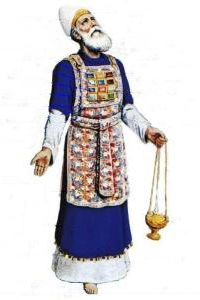
\includegraphics[width=50mm,scale=1.5]{Extras/Melchisedec.jpg}
\vspace{0.4in}  % Create a title for the document and write it in bold font
\LARGE{\textbf{\date}} % Again, do a line break
\linebreak 
% Create a subtitle \large{with Outlines, Statistics, Cross References, and Notes}
\vspace{0.5in}
\begin{flushleft}
\LARGE{Day \#50: Saturday, 19 February 2022  \\}\vspace{0.25in}
\LARGE{Numbers 28-30 Psalm 50 Proverb 19}
\end{flushleft}
\vspace{0.6in}
\bigskip

\normalsize{Xenia, Oh.\\}
\normalsize{created: \today}
\vspace{1.3in}

\end{flushright}
\end{titlepage}

\newpage 
\tableofcontents\hypertarget{TOC}{}
\listoffigures
\listoftables

\hyphenation{A-bim-e-lech bre-thren E-phra-im  Gib-e-o-nites Jer-u-sa-lem through-out Phil-i-stines The-o-phil-us Am-a-le-kites ven-geance Mesh-el-e-mi-ah onan-ism Phar-a-oh thoughts grev-ous-ness Hach-a-liah adul-ter-er Shad-rach}

%%%%%%%%%%%%%%%%% EXTRA COLORS
%%%%%%%%%%%%%%%%% EXTRA COLORS
%%%%%%%%%%%%%%%%% EXTRA COLORS
\definecolor{champagne}{rgb}{0.97,0.91,0.81}
\definecolor{bone}{rgb}{0.89,0.85,0.79}

\definecolor{ForestGreen}{rgb}{0.00,0.29,0.098}
\definecolor{GIVING}{cmyk}{1,0.0,0.72,.1}

\definecolor{MLPE}{cmyk}{1,1,0,.45}
\definecolor{SOCCER}{cmyk}{.77, 0, .42, .49}
\definecolor{PAYBILL}{cmyk}{0,0.83,0.76,0.07}
\definecolor{SERMON}{cmyk}{.14,.9,0,.30} % aka seance \href{http://www.flatuicolorpicker.com/purple-cmyk-color-model/}{seance}
\definecolor{BIBLE}{cmyk}{0,.17,.74,.17}
\definecolor{WORKBLUE}{cmyk}{1, .5, 0, .6}
\definecolor{myOrange}{cmyk}{0, .4, .98, .03}
\definecolor{myTan}{cmyk}{0.0,.07,.17,.10}
\definecolor{myRed}{cmyk}{0,1,1,0}
\definecolor{myWhite}{cmyk}{0,0,0,0}
\definecolor{BLUESoD}{cmyk}{.97,.84,0,.04}
\definecolor{WHITE}{cmyk}{0,0,0,0}
\definecolor{OLDGOLD}{cmyk}{0.05,0.3,1.00,0}
\definecolor{CASTLETON}{cmyk}{1,0,0.31,0.66}
\definecolor{cadmiumgreen}{rgb}{0.0, 0.42, 0.24}
\definecolor{jungle}{rgb}{0.203,0.4882,0.1718}
\definecolor{MYGOLD}{rgb}{1,.84,0}

\definecolor{MYLIGHTGRAY}{rgb}{.85,.85,.85}

\definecolor{codegreen}{rgb}{0,0.6,0}
\definecolor{codegray}{rgb}{0.5,0.5,0.5}
\definecolor{codepurple}{rgb}{0.58,0,0.82}
\definecolor{backcolour}{rgb}{0.95,0.95,0.92}


\mdfdefinestyle{MyFrame}{%
    linecolor=blue,
    outerlinewidth=2pt,
    roundcorner=5pt,
    innertopmargin=\baselineskip,
    innerbottommargin=\baselineskip,
    innerrightmargin=10pt,
    innerleftmargin=10pt,
    backgroundcolor=gray!25!white}


\mdfdefinestyle{MyFrame2}{%
    linecolor=black,
    outerlinewidth=2pt,
    roundcorner=5pt,
    innertopmargin=\baselineskip,
    innerbottommargin=\baselineskip,
    innerrightmargin=10pt,
    innerleftmargin=10pt,
    backgroundcolor=yellow!25!white}


%%%%%
%% for PFTTIS list
%%%%%

%%% And Joseph said unto
\index[PFTTIS]{And Joseph said unto!Genesis!Gen 40:008}
\index[PFTTIS]{And Joseph said unto!Genesis!Gen 40:012}
\index[PFTTIS]{And Joseph said unto!Genesis!Gen 41:025}
\index[PFTTIS]{And Joseph said unto!Genesis!Gen 42:014}
\index[PFTTIS]{And Joseph said unto!Genesis!Gen 42:018}
\index[PFTTIS]{And Joseph said unto!Genesis!Gen 44:015}
\index[PFTTIS]{And Joseph said unto!Genesis!Gen 45:003}
\index[PFTTIS]{And Joseph said unto!Genesis!Gen 45:004}
\index[PFTTIS]{And Joseph said unto!Genesis!Gen 46:031}
\index[PFTTIS]{And Joseph said unto!Genesis!Gen 48:009}
\index[PFTTIS]{And Joseph said unto!Genesis!Gen 48:018}
\index[PFTTIS]{And Joseph said unto!Genesis!Gen 50:019}
\index[PFTTIS]{And Joseph said unto!Genesis!Gen 50:024}


%%% a shadow
\index[PFTTIS]{a shadow!1Chronicles!1Chr 029:15}
\index[PFTTIS]{a shadow!Job!Job 008:09}
\index[PFTTIS]{a shadow!Job!Job 014:02}
\index[PFTTIS]{a shadow!Job!Job 017:07}
\index[PFTTIS]{a shadow!Psalm!Psa 102:011}
\index[PFTTIS]{a shadow!Psalm!Psa 144:004}
\index[PFTTIS]{a shadow!Ecclesiastes!Eccl 006:012}
\index[PFTTIS]{a shadow!Ecclesiastes!Eccl 008:013}
\index[PFTTIS]{a shadow!Isaiah!Isa 04:006}
\index[PFTTIS]{a shadow!Isaiah!Isa 25:004}
\index[PFTTIS]{a shadow!Jonah!Jnh 04:06}
\index[PFTTIS]{a shadow!Colossians!Col 02:017}
\index[PFTTIS]{a shadow!Hebews!Heb 10:001}

%%% blessed is the man
\index[PFTTIS]{blessed is the man!Psalm!Psa 001:001}
\index[PFTTIS]{blessed is the man!Psalm!Psa 032:002}
\index[PFTTIS]{blessed is the man!Psalm!Psa 034:008}
\index[PFTTIS]{blessed is the man!Psalm!Psa 065:004}
\index[PFTTIS]{blessed is the man!Psalm!Psa 084:005}
\index[PFTTIS]{blessed is the man!Psalm!Psa 084:012}
\index[PFTTIS]{blessed is the man!Psalm!Psa 094:012}
\index[PFTTIS]{blessed is the man!Psalm!Psa 112:001}
\index[PFTTIS]{blessed is the man!Proverbs!Pro 008:034}
\index[PFTTIS]{blessed is the man!Isaiah!Isa 056:002}
\index[PFTTIS]{blessed is the man!Jeremiah!Jer 017:007}
\index[PFTTIS]{blessed is the man!Romans!Rom 004:008}
\index[PFTTIS]{blessed is the man!James!Jam 001:012}


%%% carry them
\index[PFTTIS]{carry them!Leviticus!Lev 14:045}
\index[PFTTIS]{carry them!Numbers!Num 11:012}
\index[PFTTIS]{carry them!Joshua!Jsh 04:003}
\index[PFTTIS]{carry them!1Samuel!1Sam 20:040}
\index[PFTTIS]{carry them!1Kings!1Kng 08:046}
\index[PFTTIS]{carry them!2Chronicles!2Chr 06:036}
\index[PFTTIS]{carry them!Ezra!Ezra 05:015}
\index[PFTTIS]{carry them!Isaiah!Isa 40:011}
\index[PFTTIS]{carry them!Isaiah!Isa 41:016}
\index[PFTTIS]{carry them!Isaiah!Isa 57:013}
\index[PFTTIS]{carry them!Jeremiah!Jer 20:004}
\index[PFTTIS]{carry them!Jeremiah!Jer 20:005}
\index[PFTTIS]{carry them!Jeremiah!Jer 43:012}


\index[PFTTIS]{good tidings!2Samuel!2Sam 18:027}
\index[PFTTIS]{good tidings!1Kings!1Ki 01:042}
\index[PFTTIS]{good tidings!2Kings!2Ki 07:009 (2x)}
\index[PFTTIS]{good tidings!Isaiah!Isa 40:009 (2x)}
\index[PFTTIS]{good tidings!Isaiah!Isa 41:007}
\index[PFTTIS]{good tidings!Isaiah!Isa 52:007}
\index[PFTTIS]{good tidings!Isaiah!Isa 61:001}
\index[PFTTIS]{good tidings!Nahum!Nah 01:005}
\index[PFTTIS]{good tidings!Luke!Lk 02:010}
\index[PFTTIS]{good tidings!1Thessalonians!1Thess 03:006}


%%% dead body
\index[PFTTIS]{dead body!Leviticus!Lev 21:011}
\index[PFTTIS]{dead body!Numbers!Num 06:006}
\index[PFTTIS]{dead body!Numbers!Num 09:006}
\index[PFTTIS]{dead body!Numbers!Num 09:007}
\index[PFTTIS]{dead body!Numbers!Num 09:010}
\index[PFTTIS]{dead body!Numbers!Num 09:011}
\index[PFTTIS]{dead body!Numbers!Num 09:013}
\index[PFTTIS]{dead body!Numbers!Num 09:016}
\index[PFTTIS]{dead body!2Kings!2Ki 08:005}
\index[PFTTIS]{dead body!Isaiah!Isa 26:019}
\index[PFTTIS]{dead body!Jeremiah!Jer 26:023}
\index[PFTTIS]{dead body!Jeremiah!Jer 36:030}
\index[PFTTIS]{dead body!Haggai!Hag 02:013}

%%% great sea
\index[PFTTIS]{great sea!Numbers!Num 34:006}
\index[PFTTIS]{great sea!Numbers!Num 34:007}
\index[PFTTIS]{great sea!Joshua!Jos 01:004}
\index[PFTTIS]{great sea!Joshua!Jos 09:001}
\index[PFTTIS]{great sea!Joshua!Jos 15:012}
\index[PFTTIS]{great sea!Joshua!Jos 15:047}
\index[PFTTIS]{great sea!Joshua!Jos 23:004}
\index[PFTTIS]{great sea!Ezekiel!Eze 47:010}
\index[PFTTIS]{great sea!Ezekiel!Eze 47:015}
\index[PFTTIS]{great sea!Ezekiel!Eze 47:019}
\index[PFTTIS]{great sea!Ezekiel!Eze 47:020}
\index[PFTTIS]{great sea!Ezekiel!Eze 48:028}
\index[PFTTIS]{great sea!Daniel!Dan 07:002}


%%% have forsaken me
\index[PFTTIS]{have forsaken me!Judges!Jdg 10:013}
\index[PFTTIS]{have forsaken me!1Samuel!1Sam 08:008}
\index[PFTTIS]{have forsaken me!1Kings!1Ki 11:033}
\index[PFTTIS]{have forsaken me!2Kings!2Ki 22:017}
\index[PFTTIS]{have forsaken me!2Chronicles!2Chr 12:005}
\index[PFTTIS]{have forsaken me!2Chronicles!2Chr 34:025}
\index[PFTTIS]{have forsaken me!Jeremiah!Jer 01:016}
\index[PFTTIS]{have forsaken me!Jeremiah!Jer 02:013}
\index[PFTTIS]{have forsaken me!Jeremiah!Jer 05:007}
\index[PFTTIS]{have forsaken me!Jeremiah!Jer 05:019}
\index[PFTTIS]{have forsaken me!Jeremiah!Jer 16:011 (2x)}
\index[PFTTIS]{have forsaken me!Jeremiah!Jer 19:004}

%%% no king
\index[PFTTIS]{no king!Judges!Jdg 17:06}
\index[PFTTIS]{no king!Judges!Jdg 18:01}
\index[PFTTIS]{no king!Judges!Jdg 19:01}
\index[PFTTIS]{no king!Judges!Jdg 21:25}
\index[PFTTIS]{no king!1Kings!1Ki 22:47}
\index[PFTTIS]{no king!2Kings!2Ki 23:25}
\index[PFTTIS]{no king!Nehemiah!Neh 13:26}
\index[PFTTIS]{no king!Psalms!Psa 033:016}
\index[PFTTIS]{no king!Proverbs!Pro 30:27}
\index[PFTTIS]{no king!Daniel!Dan 02:10}
\index[PFTTIS]{no king!Hosea!Hos 10:03}
\index[PFTTIS]{no king!Micah!Mic 04:09}
\index[PFTTIS]{no king!John!Jhn 19:15}


%%% rebellious house
\index[PFTTIS]{rebellious house!Exodus!Exo 02:005}
\index[PFTTIS]{rebellious house!Exodus!Exo 02:006}
\index[PFTTIS]{rebellious house!Exodus!Exo 02:008}
\index[PFTTIS]{rebellious house!Exodus!Exo 03:009}
\index[PFTTIS]{rebellious house!Exodus!Exo 03:026}
\index[PFTTIS]{rebellious house!Exodus!Exo 03:027}
\index[PFTTIS]{rebellious house!Exodus!Exo 12:002 (2x)}
\index[PFTTIS]{rebellious house!Exodus!Exo 12:003}
\index[PFTTIS]{rebellious house!Exodus!Exo 12:009}
\index[PFTTIS]{rebellious house!Exodus!Exo 12:025}
\index[PFTTIS]{rebellious house!Exodus!Exo 17:012}
\index[PFTTIS]{rebellious house!Exodus!Exo 24:003}

%%% seek him
\index[PFTTIS]{seek him!Deuteronomy!Deu 04:029}\index[PFTTIS]{seek him!1Samuel!1Sam 23:025}
\index[PFTTIS]{seek him!1Chronicles!1Chr 28:009}
\index[PFTTIS]{seek him!2Chronicles!1Chr 15:002}
\index[PFTTIS]{seek him!Ezra!Ezr 08:022}
\index[PFTTIS]{seek him!Psalms!Psa 022:026}
\index[PFTTIS]{seek him!Psalms!Psa 024:006}
\index[PFTTIS]{seek him!Psalms!Psa 119:002}
\index[PFTTIS]{seek him!SoS!SoS 03:002}
\index[PFTTIS]{seek him!SoS!SoS 06:001}
\index[PFTTIS]{seek him!Hosea!Hos 07:010}
\index[PFTTIS]{seek him!Amos!Amo 05:008}
\index[PFTTIS]{seek him!Hebrews!Heb 11:0063}


%%% seek ye
\index[PFTTIS]{seek ye!Isaiah!Isa 34:016}
\index[PFTTIS]{seek ye!Isaiah!Isa 45:019}
\index[PFTTIS]{seek ye!Isaiah!Isa 55:006}
\index[PFTTIS]{seek ye!Amos!Amos 5:004}
\index[PFTTIS]{seek ye!John!John 1:38}
\index[PFTTIS]{seek ye!John!John 18:4}
\index[PFTTIS]{seek ye!John!John 18:7}
\index[PFTTIS]{seek ye!Matthew!Matt 6:33}
\index[PFTTIS]{seek ye!Numbers!Num 16:10}
\index[PFTTIS]{seek ye!Luke!Luke 12:31}
\index[PFTTIS]{seek ye!Luke!Luke 24:5}
\index[PFTTIS]{seek ye!Psalm!Psa 27:8}
\index[PFTTIS]{seek ye!Zephaniah!Zeph 2:3}

%%% the uncircumcised
\index[PFTTIS]{the uncircumcised!Genesis!Gen 17:014}
\index[PFTTIS]{the uncircumcised!Judges!Jdg 14:003}
\index[PFTTIS]{the uncircumcised!Judges!Jdg 15:018}
\index[PFTTIS]{the uncircumcised!2Samuel!2Sam 01:020}
\index[PFTTIS]{the uncircumcised!Isaiah!Isa 02:001}
\index[PFTTIS]{the uncircumcised!Jeremiah!Jer 09:025}
\index[PFTTIS]{the uncircumcised!Ezekiel!Eze 28:010}
\index[PFTTIS]{the uncircumcised!Ezekiel!Eze 31:018}
\index[PFTTIS]{the uncircumcised!Ezekiel!Eze 32:019}
\index[PFTTIS]{the uncircumcised!Ezekiel!Eze 32:027}
\index[PFTTIS]{the uncircumcised!Ezekiel!Eze 32:028}
\index[PFTTIS]{the uncircumcised!Ezekiel!Eze 32:029}
\index[PFTTIS]{the uncircumcised!Ezekiel!Eze 32:032}

%%% worship him
\index[PFTTIS]{worship him!Psalms!Psa 97:007}
\index[PFTTIS]{worship him!Zephaniah!Zeph 02:011}
\index[PFTTIS]{worship him!Matthew!Matt 02:002}
\index[PFTTIS]{worship him!Matthew!Matt 02:008}
\index[PFTTIS]{worship him!John!John 04:023}
\index[PFTTIS]{worship him!John!John 04:024 (2x)} 
\index[PFTTIS]{worship him!Acts!Acts 17:023}
\index[PFTTIS]{worship him!Hebrews!Heb 01:006}
\index[PFTTIS]{worship him!Revelation!Rev 04:010}
\index[PFTTIS]{worship him!Revelation!Rev 13:008}
\index[PFTTIS]{worship him!Revelation!Rev 14:007}
\index[PFTTIS]{worship him!Revelation!Rev 19:010}


%%%%%
%% for PFTTIS list
%%%%%

%%% afflictions
\index[WFTTIS]{afflictions!Psalms!Psa 34:019}
\index[WFTTIS]{afflictions!Psalms!Psa 132:001}
\index[WFTTIS]{afflictions!Acts!Acts 07:010}
\index[WFTTIS]{afflictions!Acts!Acts 20:023}
\index[WFTTIS]{afflictions!2Corinthians!2Cor 06:004}
\index[WFTTIS]{afflictions!Colossians!Col 01:024}
\index[WFTTIS]{afflictions!1Thessalonians!1Thess 03:003}
\index[WFTTIS]{afflictions!2Timothy!2Tim 01:008}
\index[WFTTIS]{afflictions!2Timothy!2Tim 03:011}
\index[WFTTIS]{afflictions!2Timothy!2Tim 04:005}
\index[WFTTIS]{afflictions!Hebrews!Heb 10:032}
\index[WFTTIS]{afflictions!Hebrews!Heb 10:033}
\index[WFTTIS]{afflictions!1Peter!1Pet 05:009}

%%% acsend
\index[WFTTIS]{acsend!Joshua!Jos 06:05}
\index[WFTTIS]{acsend!Psalm!Psa 024:003}
\index[WFTTIS]{acsend!Psalm!Psa 135:007}
\index[WFTTIS]{acsend!Psalm!Psa 139:008}
\index[WFTTIS]{acsend!Isaiah!Isa 14:013}
\index[WFTTIS]{acsend!Isaiah!Isa 14:014}
\index[WFTTIS]{acsend!Jeremiah!Jer 10:013}
\index[WFTTIS]{acsend!Jeremiah!Jer 51:016}
\index[WFTTIS]{acsend!Ezekiel!Eze 38:009}
\index[WFTTIS]{acsend!John!John 06:062}
\index[WFTTIS]{acsend!John!John 20:017}
\index[WFTTIS]{acsend!Romans!Rom 10:006}
\index[WFTTIS]{acsend!Revelation!Rev 17:008}

%%% Assyrian
\index[WFTTIS]{Assyrian!Isaiah!Isa 10:005}
\index[WFTTIS]{Assyrian!Isaiah!Isa 10:024}
\index[WFTTIS]{Assyrian!Isaiah!Isa 14:025}
\index[WFTTIS]{Assyrian!Isaiah!Isa 19:023}
\index[WFTTIS]{Assyrian!Isaiah!Isa 23:013}
\index[WFTTIS]{Assyrian!Isaiah!Isa 30:031}
\index[WFTTIS]{Assyrian!Isaiah!Isa 31:008}
\index[WFTTIS]{Assyrian!Isaiah!Isa 52:004}
\index[WFTTIS]{Assyrian!Ezekiel!Eze 31:003}
\index[WFTTIS]{Assyrian!Hosea!Hos 05:013}
\index[WFTTIS]{Assyrian!Hosea!Hos 11:005}
\index[WFTTIS]{Assyrian!Micah!Hos 05:005}
\index[WFTTIS]{Assyrian!Micah!Hos 05:006}

%%% blot
\index[WFTTIS]{blot!Exodus!Exo 32:032}
\index[WFTTIS]{blot!Exodus!Exo 32:033}
\index[WFTTIS]{blot!Numbers!Num 05:026}
\index[WFTTIS]{blot!Deuteronomy!Deut 09:014}
\index[WFTTIS]{blot!Deuteronomy!Deut 25:019}
\index[WFTTIS]{blot!Deuteronomy!Deut 29:020}
\index[WFTTIS]{blot!2Kings!2Ki 14:027}
\index[WFTTIS]{blot!Job!Job 31:007}
\index[WFTTIS]{blot!Psalms!Psa 51:001}
\index[WFTTIS]{blot!Psalms!Psa 51:009}
\index[WFTTIS]{blot!Proverbs!Pro 09:007}
\index[WFTTIS]{blot!Jeremiah!Jer 18:023}
\index[WFTTIS]{blot!Revelation!Rev 03:005}


%%% chain
\index[WFTTIS]{chain!Genesis!Gen 41:042}
\index[WFTTIS]{chain!1Kings!1Ki 07:017}
\index[WFTTIS]{chain!Psalms!Psa 73:006}
\index[WFTTIS]{chain!SoS!Sos 04:009}
\index[WFTTIS]{chain!Lamentations!Lam 03:007}
\index[WFTTIS]{chain!Ezekiel!Eze 07:023}
\index[WFTTIS]{chain!Ezekiel!Eze 16:011}
\index[WFTTIS]{chain!Daniel!Dan 05:007}
\index[WFTTIS]{chain!Daniel!Dan 05:016}
\index[WFTTIS]{chain!Daniel!Dan 05:029}
\index[WFTTIS]{chain!Acts!Acts 28:020}
\index[WFTTIS]{chain!2Timothy!2Tim 01:016}
\index[WFTTIS]{chain!Revelation!Rev 20:001}


%%% controversy
\index[WFTTIS]{controversy!Deuteronomy!Deu 17:008}
\index[WFTTIS]{controversy!Deuteronomy!Deu 19:017}
\index[WFTTIS]{controversy!Deuteronomy!Deu 21:005}
\index[WFTTIS]{controversy!Deuteronomy!Deu 25:001}
\index[WFTTIS]{controversy!2Samuel!2Sam 15:002}
\index[WFTTIS]{controversy!Isaiah!Isa 34:008}
\index[WFTTIS]{controversy!Jeremiah!Jer 25:031}
\index[WFTTIS]{controversy!Ezekiel!Eze 44:024}
\index[WFTTIS]{controversy!Hosea!Hos 04:001}
\index[WFTTIS]{controversy!Hosea!Hos 12:002}
\index[WFTTIS]{controversy!Micah!Mic 06:002 (2x)}
\index[WFTTIS]{controversy!1Timothy!1Tim 03:016}


%%% Dagon/Dagon's
\index[WFTTIS]{Dagon!Judges!Jdg 16:023}
\index[WFTTIS]{Dagon!1Samuel!1Sam 05:002 (2x)}
\index[WFTTIS]{Dagon!1Samuel!1Sam 05:003 (2x)}
\index[WFTTIS]{Dagon!1Samuel!1Sam 05:004 (3x)}
\index[WFTTIS]{Dagon!1Samuel!1Sam 05:005 (3x)}
\index[WFTTIS]{Dagon!1Samuel!1Sam 05:007}
\index[WFTTIS]{Dagon!1Chronicles!1Chr 10:010}

%%% disobedient
\index[WFTTIS]{disobedient!1Kings!1Ki 13:026}
\index[WFTTIS]{disobedient!Nehemiah!Neh 09:026}
\index[WFTTIS]{disobedient!Luke!Luke 01:017}
\index[WFTTIS]{disobedient!Acts!Acts 26:019}
\index[WFTTIS]{disobedient!Romans!Rom 01:030}
\index[WFTTIS]{disobedient!Romans!Rom 10:021}
\index[WFTTIS]{disobedient!1Timothy!1Tim 01:009}
\index[WFTTIS]{disobedient!2Timothy!2Tim 03:002}
\index[WFTTIS]{disobedient!Titus!Titus 01:016}
\index[WFTTIS]{disobedient!Titus!Titus 03:003}
\index[WFTTIS]{disobedient!1Peter!1Pet 02:007}
\index[WFTTIS]{disobedient!1Peter!1Pet 02:008}
\index[WFTTIS]{disobedient!1Peter!1Pet 03:020}


%%% doubt
\index[WFTTIS]{doubt!Genesis!Gen 37:033}
\index[WFTTIS]{doubt!Deuteronomy!Deu 28:066}
\index[WFTTIS]{doubt!Job!Job 12:002}
\index[WFTTIS]{doubt!Matthew!Matt 14:031}
\index[WFTTIS]{doubt!Matthew!Matt 21:021}
\index[WFTTIS]{doubt!Mark!Mk 11:023}
\index[WFTTIS]{doubt!Luke!Lk 11:020}
\index[WFTTIS]{doubt!John!Jhn 10:024}
\index[WFTTIS]{doubt!Acts!Acts 02:012}
\index[WFTTIS]{doubt!Acts!Acts 28:004}
\index[WFTTIS]{doubt!1Corinthians!1Cor 09:010}
\index[WFTTIS]{doubt!Galatians!Gal 04:020}
\index[WFTTIS]{doubt!1John!1Jhn 02:019}


%%% dungeon
\index[WFTTIS]{dungeon!Genesis!Gen 40:015}
\index[WFTTIS]{dungeon!Genesis!Gen 41:014}
\index[WFTTIS]{dungeon!Exodus!Exo 12:029}
\index[WFTTIS]{dungeon!Jeremiah!Jer 37:016}
\index[WFTTIS]{dungeon!Jeremiah!Jer 38:006 (2x)}
\index[WFTTIS]{dungeon!Jeremiah!Jer 38:007}
\index[WFTTIS]{dungeon!Jeremiah!Jer 38:009}
\index[WFTTIS]{dungeon!Jeremiah!Jer 38:010}
\index[WFTTIS]{dungeon!Jeremiah!Jer 38:011}
\index[WFTTIS]{dungeon!Jeremiah!Jer 38:013}
\index[WFTTIS]{dungeon!Lamentations!Lam 03:053}
\index[WFTTIS]{dungeon!Lamentations!Lam 03:055}


%%% error
\index[WFTTIS]{error!2Samuel!2Sam 06:007}
\index[WFTTIS]{error!Job!Job 19:004}
\index[WFTTIS]{error!Ecclesiastes!Ecc 05:006}
\index[WFTTIS]{error!Ecclesiastes!Ecc 10:005}
\index[WFTTIS]{error!Isaiah!Isa 32:006}
\index[WFTTIS]{error!Daniel!Dan 06:004}
\index[WFTTIS]{error!Matthew!Matt 27:064}
\index[WFTTIS]{error!Romans!Rom 01:027}
\index[WFTTIS]{error!James!Jam 05:020}
\index[WFTTIS]{error!2Peter!2Pet 02:018}
\index[WFTTIS]{error!2Peter!2Pet 03:017}
\index[WFTTIS]{error!1John!1Jn 04:006}
\index[WFTTIS]{error!Jude!Jude 01:011}

%%% fourish
\index[WFTTIS]{fourish!Psalms!Psa 072:007}
\index[WFTTIS]{fourish!Psalms!Psa 072:016}
\index[WFTTIS]{fourish!Psalms!Psa 092:007}
\index[WFTTIS]{fourish!Psalms!Psa 092:012}
\index[WFTTIS]{fourish!Psalms!Psa 092:013}
\index[WFTTIS]{fourish!Psalms!Psa 132:018}
\index[WFTTIS]{fourish!Proverbs!Pro 11:28}
\index[WFTTIS]{fourish!Proverbs!Pro 14:11}
\index[WFTTIS]{fourish!Ecclesiastes!Ecc 12:05}
\index[WFTTIS]{fourish!SongOfSolomon!SOS 07:12}
\index[WFTTIS]{fourish!Isaiah!Isa 17:11}
\index[WFTTIS]{fourish!Isaiah!Isa 66:14}
\index[WFTTIS]{fourish!Ezekiel!Eze 17:24}




%%% giants
\index[WFTTIS]{giants!Genesis!Gen 06:004}
\index[WFTTIS]{giants!Numbers!Num 13:033}
\index[WFTTIS]{giants!Deuteronomy!Deut 02:011}
\index[WFTTIS]{giants!Deuteronomy!Deut 02:021}
\index[WFTTIS]{giants!Deuteronomy!Deut 03:011}
\index[WFTTIS]{giants!Deuteronomy!Deut 03:013}
\index[WFTTIS]{giants!Joshua!Josh 12:004}
\index[WFTTIS]{giants!Joshua!Josh 13:012}
\index[WFTTIS]{giants!Joshua!Josh 15:008}
\index[WFTTIS]{giants!Joshua!Josh 17:015}
\index[WFTTIS]{giants!Joshua!Josh 16:016}

%%% good man
\index[WFTTIS]{good man!2 Samuel!2Sa 18:27}
%(1) Psalms 37:23 [5]
%(1) Psalms 112:5 [2]
%(1) Proverbs 12:2 [2]
%(1) Proverbs 13:22 [2]
%(1) Proverbs 14:14 [14]
%(1) Micah 7:2 [2]
%(1) Matthew 12:35 [2]
%(1) Luke 6:45 [2]
%(1) Luke 23:50 [15]
%(1) John 7:12 [17]
%(1) Acts 11:24 [5]
%(1) Romans 5:7 [14]

%%% Hinnom
\index[WFTTIS]{Hinnom!Joshua!Jsh 15:008}
\index[WFTTIS]{Hinnom!Joshua!Jsh 18:016}
\index[WFTTIS]{Hinnom!2Kings!2Ki 23:010}
\index[WFTTIS]{Hinnom!2Chronicles!2Chr 28:003}
\index[WFTTIS]{Hinnom!2Chronicles!2Chr 33:006}
\index[WFTTIS]{Hinnom!Nehemiah!Neh 11:030}
\index[WFTTIS]{Hinnom!Jeremiah!Jer 07:031}
\index[WFTTIS]{Hinnom!Jeremiah!Jer 07:032}
\index[WFTTIS]{Hinnom!Jeremiah!Jer 19:002}
\index[WFTTIS]{Hinnom!Jeremiah!Jer 19:006}
\index[WFTTIS]{Hinnom!Jeremiah!Jer 32:035}

%%% inclined
\index[WFTTIS]{inclined!Judges!Jdg 09:003}
\index[WFTTIS]{inclined!Psalms!Psa 040:001}
\index[WFTTIS]{inclined!Psalms!Psa 116:002}
\index[WFTTIS]{inclined!Psalms!Psa 119:112}
\index[WFTTIS]{inclined!Proverbs!Pro 05:13}
\index[WFTTIS]{inclined!Jeremiah!Jer 07:24}
\index[WFTTIS]{inclined!Jeremiah!Jer 07:26}
\index[WFTTIS]{inclined!Jeremiah!Jer 11:08}
\index[WFTTIS]{inclined!Jeremiah!Jer 17:23}
\index[WFTTIS]{inclined!Jeremiah!Jer 25:04}
\index[WFTTIS]{inclined!Jeremiah!Jer 34:14}
\index[WFTTIS]{inclined!Jeremiah!Jer 35:15}
\index[WFTTIS]{inclined!Jeremiah!Jer 44:05}


%%% laughed
\index[WFTTIS]{laughed!Genesis!Gen 17:017}
\index[WFTTIS]{laughed!Genesis!Gen 18:012}
\index[WFTTIS]{laughed!Genesis!Gen 18:015}
\index[WFTTIS]{laughed!2Kings!2Ki 19:021}
\index[WFTTIS]{laughed!2Chronicles!2Chr 30:010}
\index[WFTTIS]{laughed!Nehemiah!Neh 02:019}
\index[WFTTIS]{laughed!Job!Job 12:004}
\index[WFTTIS]{laughed!Job!Job 29:024}
\index[WFTTIS]{laughed!Isaiah!Isa 37:022}
\index[WFTTIS]{laughed!Ezekiel!Ezek 23:032}
\index[WFTTIS]{laughed!Matthew!Matt 09:024}
\index[WFTTIS]{laughed!Mark!Mk 05:040}
\index[WFTTIS]{laughed!Luke!Lk 08:053}

%%% liar
\index[WFTTIS]{liar!Job!Job 24:025}
\index[WFTTIS]{liar!Proverbs!Pro 17:004}
\index[WFTTIS]{liar!Proverbs!Pro 19:022}
\index[WFTTIS]{liar!Proverbs!Pro 30:006}
\index[WFTTIS]{liar!Jeremiah!Jer 15:018}
\index[WFTTIS]{liar!John!Jhn 08:044}
\index[WFTTIS]{liar!John!Jhn 08:055}
\index[WFTTIS]{liar!Romans!Rom 03:004}
\index[WFTTIS]{liar!1John!1Jhn 01:010}
\index[WFTTIS]{liar!1John!1Jhn 02:004}
\index[WFTTIS]{liar!1John!1Jhn 02:022}
\index[WFTTIS]{liar!1John!1Jhn 04:020}
\index[WFTTIS]{liar!1John!1Jhn 05:010}

%%% palsy
\index[WFTTIS]{palsy!Matthew!Matt 04:024}
\index[WFTTIS]{palsy!Matthew!Matt 08:006}
\index[WFTTIS]{palsy!Matthew!Matt 09:002}
\index[WFTTIS]{palsy!Matthew!Matt 09:006}
\index[WFTTIS]{palsy!Mark!Mk 02:003}
\index[WFTTIS]{palsy!Mark!Mk 02:004}
\index[WFTTIS]{palsy!Mark!Mk 02:005}
\index[WFTTIS]{palsy!Mark!Mk 02:009}
\index[WFTTIS]{palsy!Mark!Mk 02:010}
\index[WFTTIS]{palsy!Luke!Lk 05:018}
\index[WFTTIS]{palsy!Luke!Lk 05:024}
\index[WFTTIS]{palsy!Acts!Acts 09:033}

%%% Profitable
\index[WFTTIS]{profitable!Job!Job 22:002 (2x)}
\index[WFTTIS]{profitable!Ecclesiastes!Ecc 10:010}
\index[WFTTIS]{profitable!Isaiah!Isa 44:010}
\index[WFTTIS]{profitable!Jeremiah!Jer 13:007}
\index[WFTTIS]{profitable!Matthew!Matt 05:029}
\index[WFTTIS]{profitable!Matthew!Matt 05:030}
\index[WFTTIS]{profitable!Acts!Acts 20:020}
\index[WFTTIS]{profitable!1Timothy!1Tim 04:008}
\index[WFTTIS]{profitable!2Timothy!2Tim 03:016}
\index[WFTTIS]{profitable!2Timothy!2Tim 04:011}
\index[WFTTIS]{profitable!Titus!Titus 03:008}
\index[WFTTIS]{profitable!Philemon!Phlm 01:011}

%%% Rechab
\index[WFTTIS]{Rechab!2Samuel!2Sam 04:002}
\index[WFTTIS]{Rechab!2Samuel!2Sam 04:005}
\index[WFTTIS]{Rechab!2Samuel!2Sam 04:006}
\index[WFTTIS]{Rechab!2Samuel!2Sam 04:009}
\index[WFTTIS]{Rechab!2KIngs!2Ki 10:015}
\index[WFTTIS]{Rechab!2KIngs!2Ki 10:023}
\index[WFTTIS]{Rechab!1Chronicles!1Chr 02:055}
\index[WFTTIS]{Rechab!Nehemiah!Neh 03:014}
\index[WFTTIS]{Rechab!Jeremiah!Jer 35:006}
\index[WFTTIS]{Rechab!Jeremiah!Jer 35:008}
\index[WFTTIS]{Rechab!Jeremiah!Jer 35:014}
\index[WFTTIS]{Rechab!Jeremiah!Jer 35:016}
\index[WFTTIS]{Rechab!Jeremiah!Jer 35:019}

%%% serpents
\index[WFTTIS]{serpents!Exodus!Exo 07:012}
\index[WFTTIS]{serpents!Numbers!Num 21:006}
\index[WFTTIS]{serpents!Numbers!Num 21:007}
\index[WFTTIS]{serpents!Deuteronomy!Deu 08:015}
\index[WFTTIS]{serpents!Deuteronomy!Deu 32:024}
\index[WFTTIS]{serpents!Jeremiah!Jer 08:017}
\index[WFTTIS]{serpents!Matthew!Matt 10:016}
\index[WFTTIS]{serpents!Matthew!Matt 23:033}
\index[WFTTIS]{serpents!Mark!Mk 16:018}
\index[WFTTIS]{serpents!Luke!Lk 10:019}
\index[WFTTIS]{serpents!1Corinthians!1Cor 10:009}
\index[WFTTIS]{serpents!James!Jas 03:007}
\index[WFTTIS]{serpents!Revelation!Rev 09:019}

%%% short
\index[WFTTIS]{short!Numbers!Num 11:023}
\index[WFTTIS]{short!2Kings!2Ki 10:032}
\index[WFTTIS]{short!Job!Job 17:012}
\index[WFTTIS]{short!Job!Job 20:005}
\index[WFTTIS]{short!Psalms!Psa 89:047}
\index[WFTTIS]{short!Romans!Rom 03:023}
\index[WFTTIS]{short!Romans!Rom 09:028  (2x)}
\index[WFTTIS]{short!1Corinthians!1Cor 07:029}
\index[WFTTIS]{short!1Thessalonians!1Thess 02:017}
\index[WFTTIS]{short!Hebrews!Heb 04:001}
\index[WFTTIS]{short!Revelation!Rev 12:012}
\index[WFTTIS]{short!Revelation!Rev 17:010}

%%% smiteth
\index[WFTTIS]{smiteth!Exodus!Exo 21:012}
\index[WFTTIS]{smiteth!Exodus!Exo 21:15}
\index[WFTTIS]{smiteth!Deuteronomy!Dt 25:11}
\index[WFTTIS]{smiteth!Deuteronomy!Dt 27:24}
\index[WFTTIS]{smiteth!Joshua!Jsh 15:16}
\index[WFTTIS]{smiteth!Judges!Jdg 15:16}
\index[WFTTIS]{smiteth!2 Samuel!2Sa 05:08}
\index[WFTTIS]{smiteth!1Chronicles!1Chr 11:06}
\index[WFTTIS]{smiteth!Job!1Chr 26:12}
\index[WFTTIS]{smiteth!Isaiah!Isa 09:13}
\index[WFTTIS]{smiteth!Lamentations!Lam 03:30}
\index[WFTTIS]{smiteth!Ezekiel!Eze 07:09}
\index[WFTTIS]{smiteth!Luke!Lk 06:29}



%%% vanities
\index[WFTTIS]{vanities!Deuteronomy!Deut 21:021}
\index[WFTTIS]{vanities!1Kings!1Ki 16:013}
\index[WFTTIS]{vanities!1Kings!1Ki 16:026}
\index[WFTTIS]{vanities!Psalms!Psa 031:006}
\index[WFTTIS]{vanities!Ecclesiastes!Ecc 01:002 (2x)}
\index[WFTTIS]{vanities!Ecclesiastes!Ecc 05:007}
\index[WFTTIS]{vanities!Ecclesiastes!Ecc 12:008}
\index[WFTTIS]{vanities!Jeremiah!Jer 08:019}
\index[WFTTIS]{vanities!Jeremiah!Jer 10:008}
\index[WFTTIS]{vanities!Jeremiah!Jer 14:022}
\index[WFTTIS]{vanities!Jonah!Jnh 02:008}
\index[WFTTIS]{vanities!Acts!Acts 14:015}



%%%%%
%% for PFTTIS list
%%%%%

%%% worm
\index[WFITV]{worm!Exodus!Exo 16:024}
\index[WFITV]{worm!Job!Job 17:014}
\index[WFITV]{worm!Job!Job 24:029}
\index[WFITV]{worm!Job!Job 25:005 (2x)}
\index[WFITV]{worm!Psalms!Psa 022:006}
\index[WFITV]{worm!Isaiah!Isa 14:011}
\index[WFITV]{worm!Isaiah!Isa 41:014}
\index[WFITV]{worm!Isaiah!Isa 51:008}
\index[WFITV]{worm!Isaiah!Isa 66:024}
\index[WFITV]{worm!Jonah!Jnh 04:007}
\index[WFITV]{worm!Mark!Mk 09:044}
\index[WFITV]{worm!Mark!Mk 09:046}
\index[WFITV]{worm!Mark!Mk 09:048}


%\subsubsection{Title}
%\textbf{Introduction:} Isaiah 46 
%\index[speaker]{Speaker!Isaiah 49 (Title}
%\index[series]{Book (Speaker)!IPassage (Title)}
%\index[date]{2017/07/09!Isaiah 49 (Title)}
%\begin{compactenum}[I.]
%    \item  \textbf{Point} \index[scripture]{Isaiah!IPassage} (IPassage)
%\end{compactenum}




  


%\input{02OT-Exodus/ExodusIntroduction}
\newpage
\begin{figure}
\begin{center}
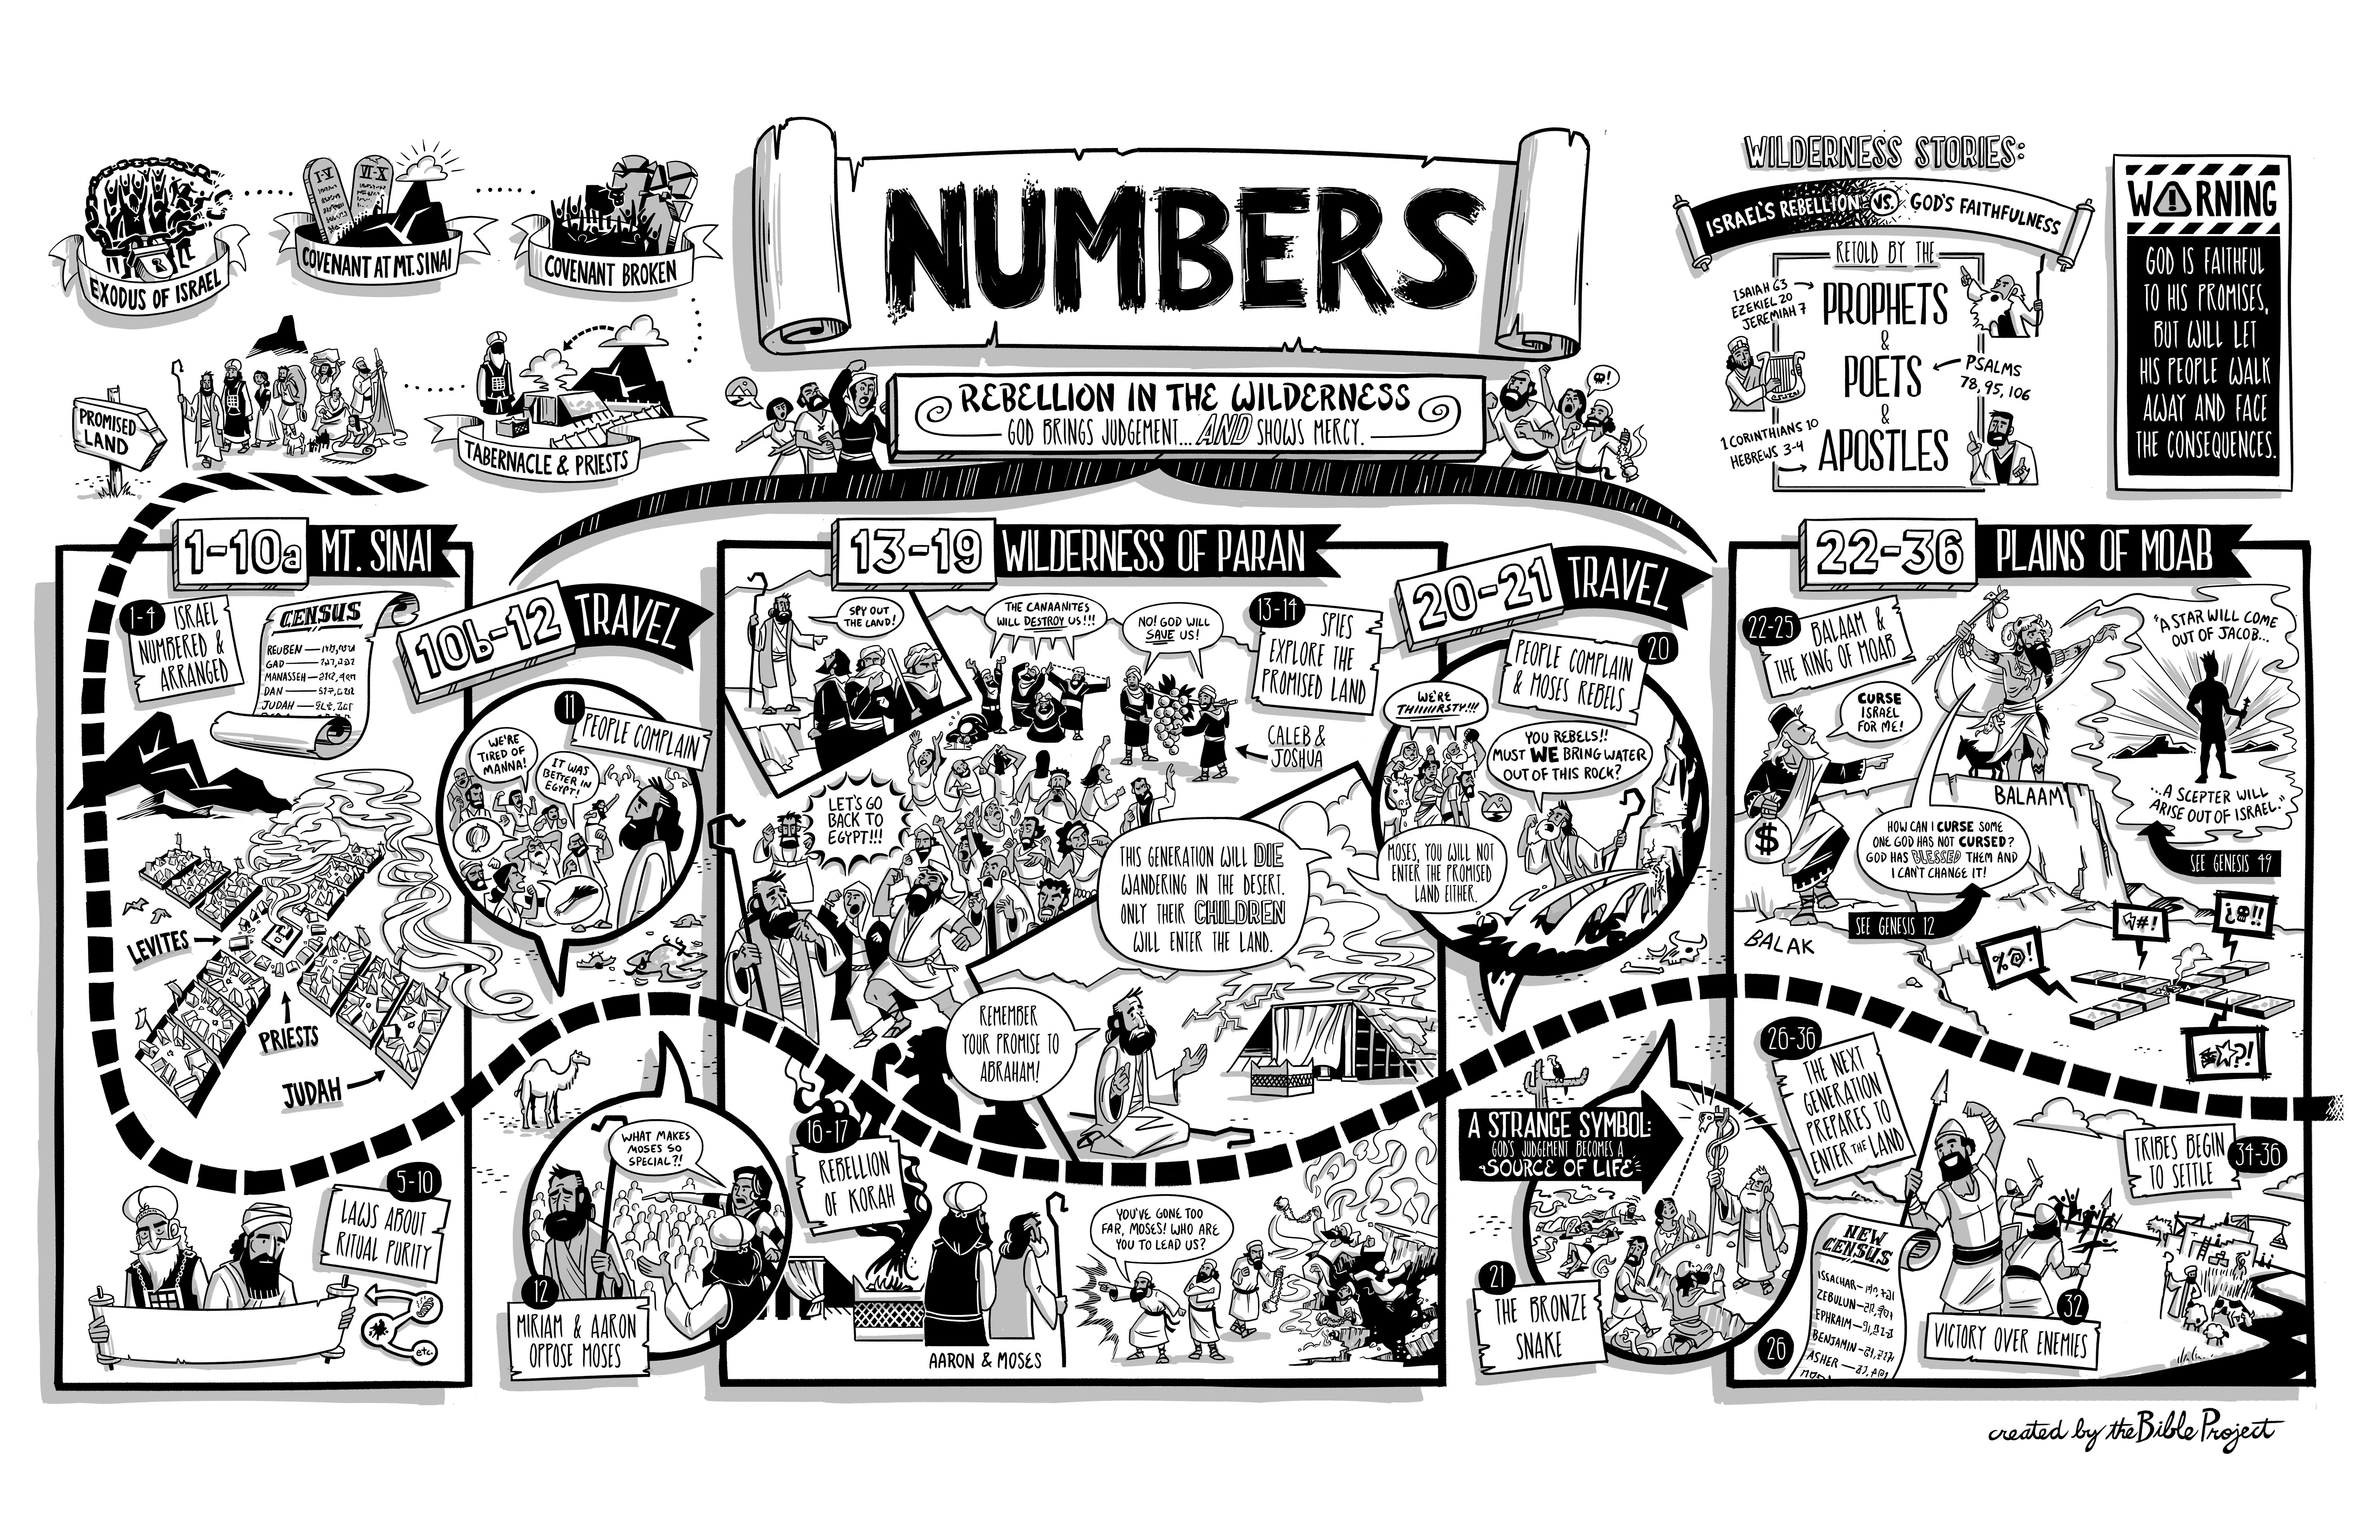
\includegraphics[scale=0.5, angle=90]{04OT-Numbers/References/BibleProject-Numbers.jpg}
\caption[Numbers from the Bible Project]{Numbers from the Bible Project}
\label{fig:Numbers from the Bible Project}
\end{center}
\end{figure}

\newpage
\begin{figure}
\begin{center}
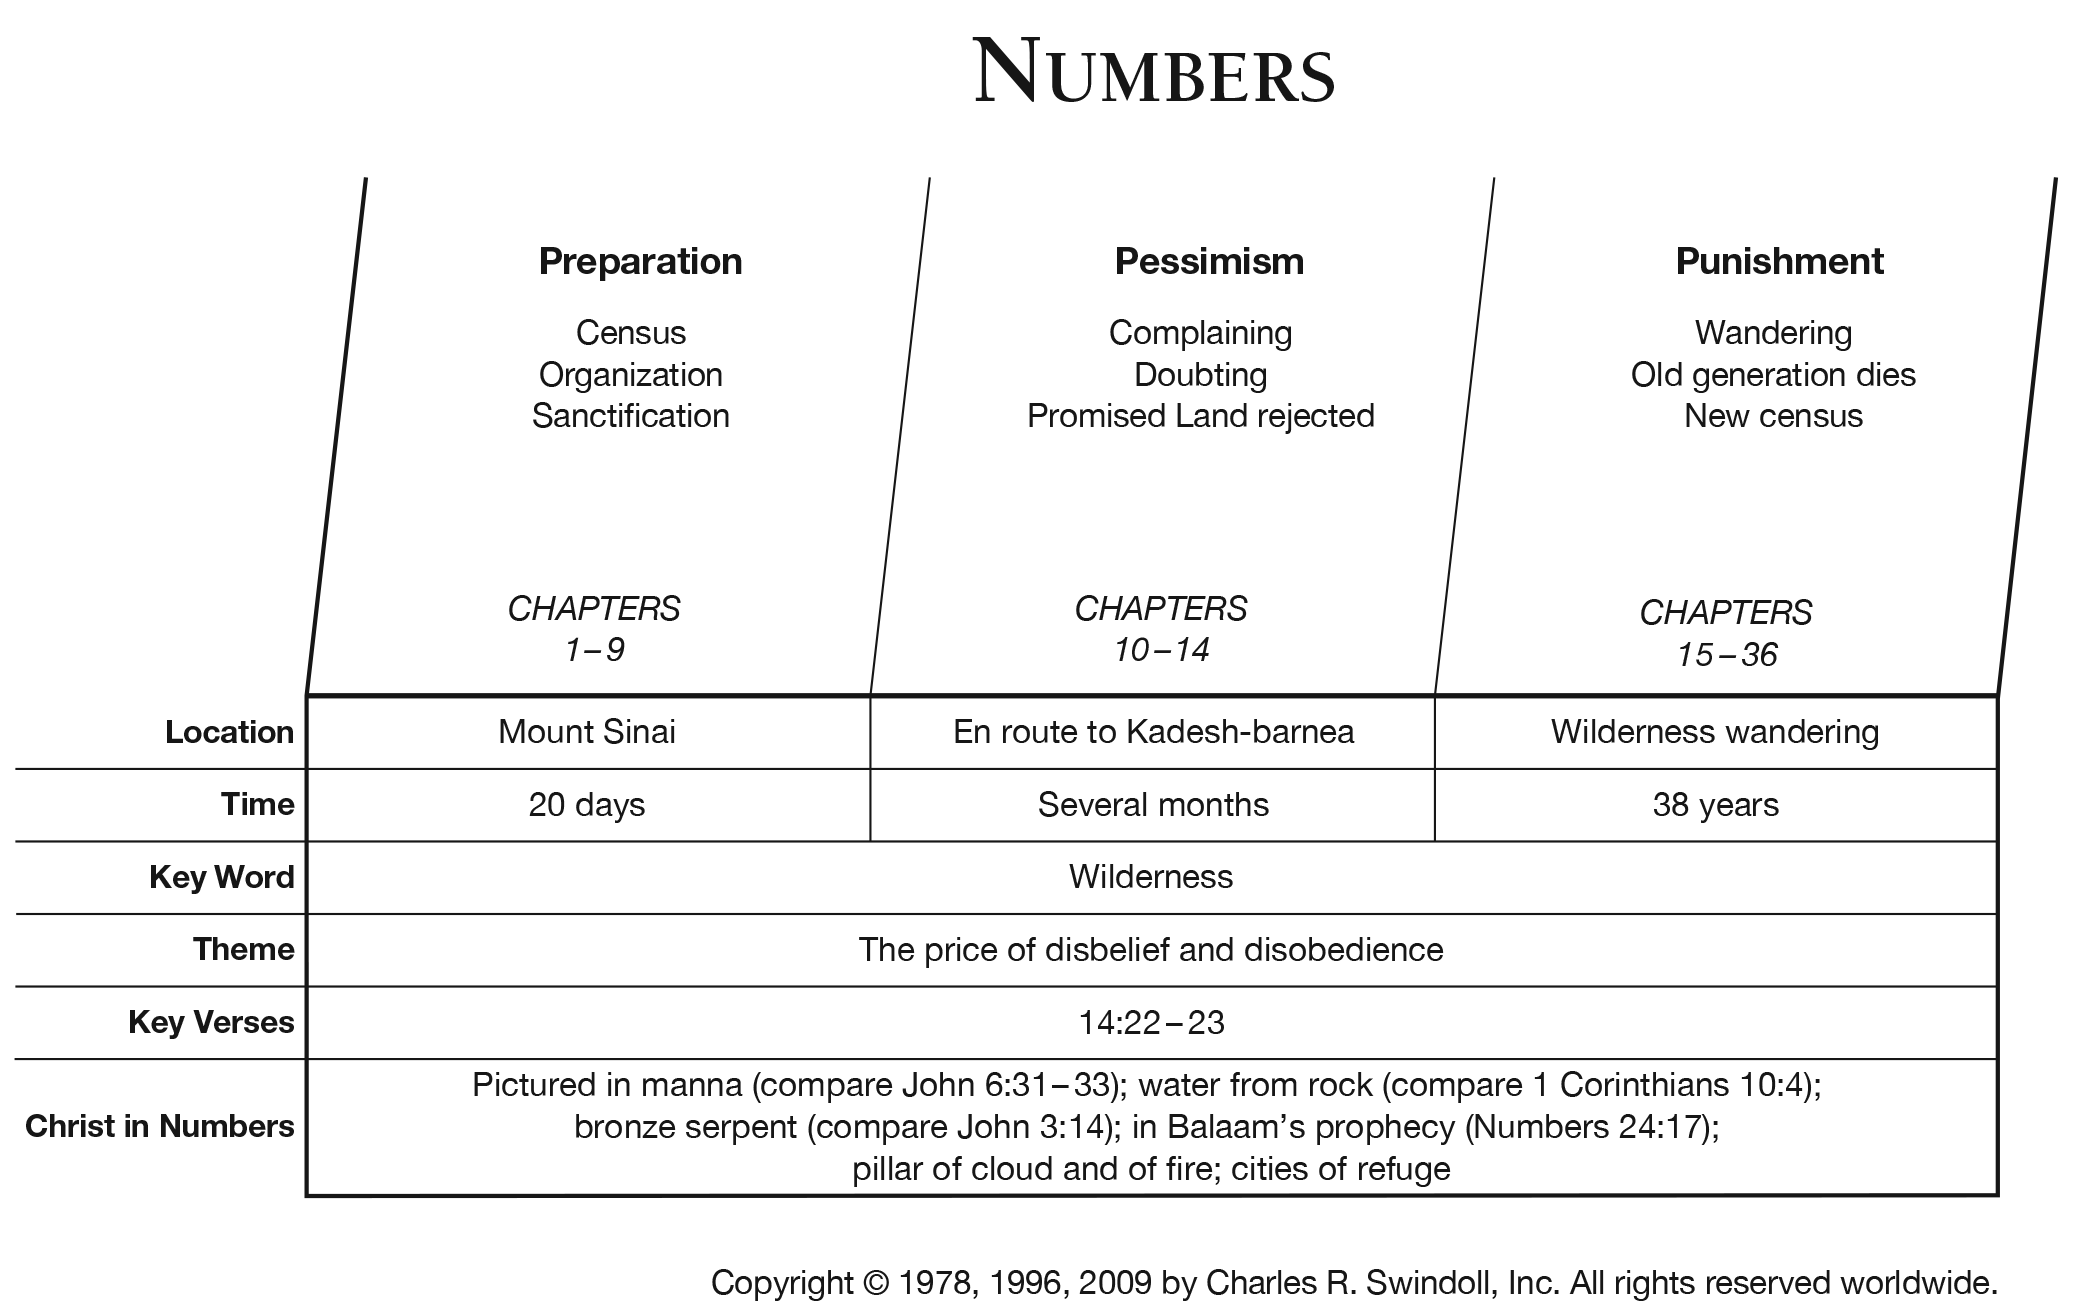
\includegraphics[scale=0.3, angle=90]{04OT-Numbers/References/Swindoll-Numbers.png}
\caption[Numbers by Swindoll]{Numbers by Swindoll}
\label{fig:Numbers by Swindoll}
\end{center}
\end{figure}

\newpage
\begin{figure}
\begin{center}
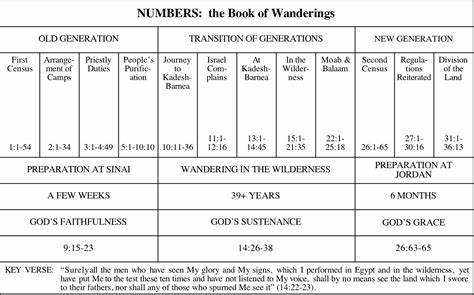
\includegraphics[scale=1.2, angle=90]{04OT-Numbers/References/Numbers.jpg}
\caption[Numbers by Unknown]{Numbers by Unknown}
\label{fig:Numbers by Unknown}
\end{center}
\end{figure}

\newpage
\begin{figure}
\begin{center}
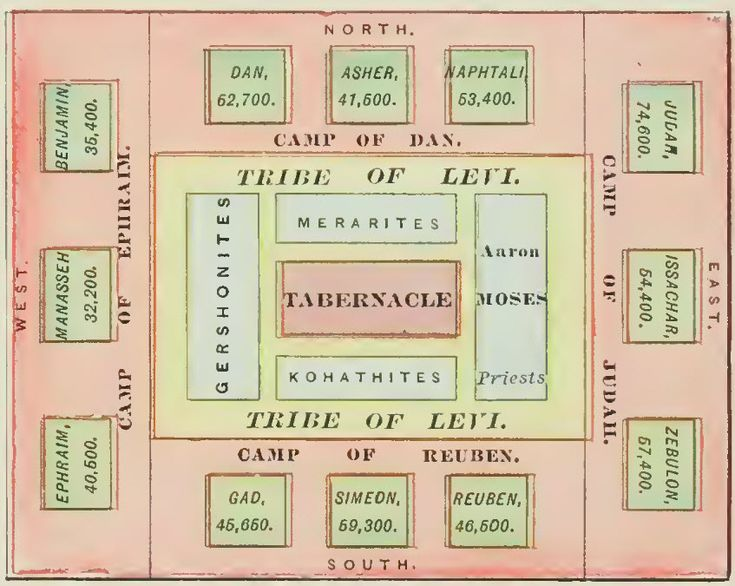
\includegraphics[scale=.8, angle=0]{04OT-Numbers/References/LayoutOfTribesAndTabernacle.jpg}
\caption[Layout of Tribes and Tabernacle]{Layout of Tribes and Tabernacle}
\label{fig:Layout of Tribes and Tabernacle}
\end{center}
\end{figure}


\chapter{Numbers 28}
%[cmyk]{0.99998,1,0,0}{


\marginpar{\scriptsize \centering \fcolorbox{bone}{lime}{\textbf{OFFERINGS \& MORE OF THEM}}\\ (Numbers 28)
\begin{compactenum}[I.][8]
    \item \textbf{Aroma} \index[scripture]{Numbers!Num 28:02}\index[scripture]{Numbers!Num 28:06} \index[scripture]{Numbers!Num 28:08}\index[scripture]{Numbers!Num 28:13}\index[scripture]{Numbers!Num 28:24}\index[scripture]{Numbers!Num 28:27}(Numbers 28:2, 6, 8, 13, 24, 27) -- sweet savour
    \item \textbf{Rituals} 
    \item \textbf{Rams} \index[scripture]{Numbers!Num 28:11}\index[scripture]{Numbers!Num 28:12} \index[scripture]{Numbers!Num 28:14}\index[scripture]{Numbers!Num 28:19}\index[scripture]{Numbers!Num 28:20}\index[scripture]{Numbers!Num 28:27}\index[scripture]{Numbers!Num 28:28}(Numbers 28:11, 12, 14, 19, 20, 27, 28) -
    \item \textbf{Repetition} -- \index[scripture]{Numbers!Num 28:31}(Numbers 28:31)
    \item \textbf{Remembrance} 
    \item \textbf{Reiteration} 
    \item \textbf{Requirement} 
    \item \textbf{Rest} \index[scripture]{Numbers!Num 28:26}(Numbers 28:26)
\end{compactenum}}

%%%%%%%%%%%%%%%%%%%%%%%%%%%%%%%%%%%%%%%%%
%%%%%%%%%%%%%%%%%%%%%%%%%%%%%%%%%%%%%%%%%
\footnote{\textcolor[rgb]{0.00,0.25,0.00}{\hyperlink{NumbersTOC}{Return to end of Table of Contents.}}}\footnote{\href{https://audiobible.com/bible/numbers_28.html}{\textcolor[cmyk]{0.99998,1,0,0}{Numbers 28 Audio}}}\textcolor[cmyk]{0.99998,1,0,0}{And \fcolorbox{bone}{bone}{the LORD} spake unto Moses, saying,}
[2] \textcolor[cmyk]{0.99998,1,0,0}{Command the children of Israel, and say unto them, My offering, \emph{and} my bread for my sacrifices made by fire, \emph{for} a sweet savour unto me, shall \fcolorbox{bone}{bone}{ye} observe to offer unto me in their due season.}
[3] \textcolor[cmyk]{0.99998,1,0,0}{And thou shalt say unto them, This \emph{is} the offering made by fire which \fcolorbox{bone}{bone}{ye} shall offer unto \fcolorbox{bone}{bone}{the LORD}; two lambs of the first year without spot day by day, \emph{for} a continual burnt offering.}
[4] \textcolor[cmyk]{0.99998,1,0,0}{The one lamb shalt thou offer in the morning, and the other lamb shalt thou offer at even;}
[5] \textcolor[cmyk]{0.99998,1,0,0}{And a tenth \emph{part} of an ephah of flour for a meat offering, mingled with the fourth \emph{part} of an hin of beaten oil.}
[6] \textcolor[cmyk]{0.99998,1,0,0}{\emph{It} \emph{is} a continual burnt offering, which was ordained in mount Sinai for a sweet savour, a sacrifice made by fire unto \fcolorbox{bone}{bone}{the LORD}.}
[7] \textcolor[cmyk]{0.99998,1,0,0}{And the drink offering thereof \emph{shall} \emph{be} the fourth \emph{part} of an hin for the one lamb: in the holy \emph{place} shalt thou cause the strong wine to be poured unto \fcolorbox{bone}{bone}{the LORD} \emph{for} a drink offering.}
[8] \textcolor[cmyk]{0.99998,1,0,0}{And the other lamb shalt thou offer at even: as the meat offering of the morning, and as the drink offering thereof, thou shalt offer \emph{it}, a sacrifice made by fire, of a sweet savour unto \fcolorbox{bone}{bone}{the LORD}.}\\
\\
\P \textcolor[cmyk]{0.99998,1,0,0}{And on the sabbath day two lambs of the first year without spot, and two tenth deals of flour \emph{for} a meat offering, mingled with oil, and the drink offering thereof:}
[10] \textcolor[cmyk]{0.99998,1,0,0}{\emph{This} \emph{is} the burnt offering of every sabbath, beside the continual burnt offering, and his drink offering.}\\
\\
\P \textcolor[cmyk]{0.99998,1,0,0}{And in the beginnings of your months \fcolorbox{bone}{bone}{ye} shall offer a burnt offering unto \fcolorbox{bone}{bone}{the} \fcolorbox{bone}{bone}{LORD}; two young bullocks, and one ram, seven lambs of the first year without spot;}
[12] \textcolor[cmyk]{0.99998,1,0,0}{And three tenth deals of flour \emph{for} a meat offering, mingled with oil, for one bullock; and two tenth deals of flour \emph{for} a meat offering, mingled with oil, for one ram;}
[13] \textcolor[cmyk]{0.99998,1,0,0}{And a several tenth deal of flour mingled with oil \emph{for} a meat offering unto one lamb; \emph{for} a burnt offering of a sweet savour, a sacrifice made by fire unto \fcolorbox{bone}{bone}{the LORD}.}
[14] \textcolor[cmyk]{0.99998,1,0,0}{And their drink offerings shall be half an hin of wine unto a bullock, and the third \emph{part} of an hin unto a ram, and a fourth \emph{part} of an hin unto a lamb: this \emph{is} the burnt offering of every month throughout the months of the year.}
[15] \textcolor[cmyk]{0.99998,1,0,0}{And one kid of the goats for a sin offering unto \fcolorbox{bone}{bone}{the LORD} shall be offered, beside the continual burnt offering, and his drink offering.}
[16] \textcolor[cmyk]{0.99998,1,0,0}{And in the fourteenth day of the first month \emph{is} the passover of \fcolorbox{bone}{bone}{the LORD}.}
[17] \textcolor[cmyk]{0.99998,1,0,0}{And in the fifteenth day of this month \emph{is} the feast: seven days shall unleavened bread be eaten.}
[18] \textcolor[cmyk]{0.99998,1,0,0}{In the first day \emph{shall} \emph{be} an holy convocation; \fcolorbox{bone}{bone}{ye} shall do no manner of servile work \emph{therein}:}
[19] \textcolor[cmyk]{0.99998,1,0,0}{But \fcolorbox{bone}{bone}{ye} shall offer a sacrifice made by fire \emph{for} a burnt offering unto \fcolorbox{bone}{bone}{the LORD}; two young bullocks, and one ram, and seven lambs of the first year: they shall be unto you without blemish:}
[20] \textcolor[cmyk]{0.99998,1,0,0}{And their meat offering \emph{shall} \emph{be} \emph{of} flour mingled with oil: three tenth deals shall \fcolorbox{bone}{bone}{ye} offer for a bullock, and two tenth deals for a ram;}
[21] \textcolor[cmyk]{0.99998,1,0,0}{A several tenth deal shalt thou offer for every lamb, throughout the seven lambs:}
[22] \textcolor[cmyk]{0.99998,1,0,0}{And one goat \emph{for} a sin offering, to make an atonement for you.}
[23] \textcolor[cmyk]{0.99998,1,0,0}{Ye shall offer these beside the burnt offering in the morning, which \emph{is} for a continual burnt offering.}
[24] \textcolor[cmyk]{0.99998,1,0,0}{After this manner \fcolorbox{bone}{bone}{ye} shall offer daily, throughout the seven days, the meat of the sacrifice made by fire, of a sweet savour unto \fcolorbox{bone}{bone}{the LORD}: it shall be offered beside the continual burnt offering, and his drink offering.}
[25] \textcolor[cmyk]{0.99998,1,0,0}{And on the seventh day \fcolorbox{bone}{bone}{ye} shall have an holy convocation; \fcolorbox{bone}{bone}{ye} shall do no servile work.}\\
\\
\P \textcolor[cmyk]{0.99998,1,0,0}{Also in the day of the firstfruits, when \fcolorbox{bone}{bone}{ye} bring a new meat offering unto \fcolorbox{bone}{bone}{the} \fcolorbox{bone}{bone}{LORD}, after your weeks \emph{be} \emph{out}, \fcolorbox{bone}{bone}{ye} shall have an holy convocation; \fcolorbox{bone}{bone}{ye} shall do no servile work:}
[27] \textcolor[cmyk]{0.99998,1,0,0}{But \fcolorbox{bone}{bone}{ye} shall offer the burnt offering for a sweet savour unto \fcolorbox{bone}{bone}{the LORD}; two young bullocks, one ram, seven lambs of the first year;}
[28] \textcolor[cmyk]{0.99998,1,0,0}{And their meat offering of flour mingled with oil, three tenth deals unto one bullock, two tenth deals unto one ram,}
[29] \textcolor[cmyk]{0.99998,1,0,0}{A several tenth deal unto one lamb, throughout the seven lambs;}
[30] \textcolor[cmyk]{0.99998,1,0,0}{\emph{And} one kid of the goats, to make an atonement for you.}
[31] \textcolor[cmyk]{0.99998,1,0,0}{Ye shall offer \emph{them} beside the continual burnt offering, and his meat offering, (they shall be unto you without blemish) and their drink offerings.}
\index[NWIV]{7!Numbers!Num 28:1}\index[AWIP]{And!Numbers!Num 28:1}\index[AWIP]{the!Numbers!Num 28:1}\index[AWIP]{LORD!Numbers!Num 28:1}\index[AWIP]{spake!Numbers!Num 28:1}\index[AWIP]{unto!Numbers!Num 28:1}\index[AWIP]{Moses!Numbers!Num 28:1}\index[AWIP]{saying!Numbers!Num 28:1}

\index[NWIV]{37!Numbers!Num 28:2}\index[AWIP]{Command!Numbers!Num 28:2}\index[AWIP]{the!Numbers!Num 28:2}\index[AWIP]{children!Numbers!Num 28:2}\index[AWIP]{of!Numbers!Num 28:2}\index[AWIP]{Israel!Numbers!Num 28:2}\index[AWIP]{and!Numbers!Num 28:2}\index[AWIP]{say!Numbers!Num 28:2}\index[AWIP]{unto!Numbers!Num 28:2}\index[AWIP]{unto!Numbers!Num 28:2 (2)}\index[AWIP]{unto!Numbers!Num 28:2 (3)}\index[AWIP]{them!Numbers!Num 28:2}\index[AWIP]{My!Numbers!Num 28:2}\index[AWIP]{offering!Numbers!Num 28:2}\index[AWIP]{\emph{and}!Numbers!Num 28:2}\index[AWIP]{my!Numbers!Num 28:2}\index[AWIP]{my!Numbers!Num 28:2 (2)}\index[AWIP]{bread!Numbers!Num 28:2}\index[AWIP]{for!Numbers!Num 28:2}\index[AWIP]{sacrifices!Numbers!Num 28:2}\index[AWIP]{made!Numbers!Num 28:2}\index[AWIP]{by!Numbers!Num 28:2}\index[AWIP]{fire!Numbers!Num 28:2}\index[AWIP]{\emph{for}!Numbers!Num 28:2}\index[AWIP]{a!Numbers!Num 28:2}\index[AWIP]{sweet!Numbers!Num 28:2}\index[AWIP]{savour!Numbers!Num 28:2}\index[AWIP]{me!Numbers!Num 28:2}\index[AWIP]{me!Numbers!Num 28:2 (2)}\index[AWIP]{shall!Numbers!Num 28:2}\index[AWIP]{ye!Numbers!Num 28:2}\index[AWIP]{observe!Numbers!Num 28:2}\index[AWIP]{to!Numbers!Num 28:2}\index[AWIP]{offer!Numbers!Num 28:2}\index[AWIP]{in!Numbers!Num 28:2}\index[AWIP]{their!Numbers!Num 28:2}\index[AWIP]{due!Numbers!Num 28:2}\index[AWIP]{season!Numbers!Num 28:2}\index[AWIP]{\emph{and}!Numbers!Num 28:2}\index[AWIP]{\emph{for}!Numbers!Num 28:2}

\index[NWIV]{36!Numbers!Num 28:3}\index[AWIP]{And!Numbers!Num 28:3}\index[AWIP]{thou!Numbers!Num 28:3}\index[AWIP]{shalt!Numbers!Num 28:3}\index[AWIP]{say!Numbers!Num 28:3}\index[AWIP]{unto!Numbers!Num 28:3}\index[AWIP]{unto!Numbers!Num 28:3 (2)}\index[AWIP]{them!Numbers!Num 28:3}\index[AWIP]{This!Numbers!Num 28:3}\index[AWIP]{\emph{is}!Numbers!Num 28:3}\index[AWIP]{the!Numbers!Num 28:3}\index[AWIP]{the!Numbers!Num 28:3 (2)}\index[AWIP]{the!Numbers!Num 28:3 (3)}\index[AWIP]{offering!Numbers!Num 28:3}\index[AWIP]{offering!Numbers!Num 28:3 (2)}\index[AWIP]{made!Numbers!Num 28:3}\index[AWIP]{by!Numbers!Num 28:3}\index[AWIP]{by!Numbers!Num 28:3 (2)}\index[AWIP]{fire!Numbers!Num 28:3}\index[AWIP]{which!Numbers!Num 28:3}\index[AWIP]{ye!Numbers!Num 28:3}\index[AWIP]{shall!Numbers!Num 28:3}\index[AWIP]{offer!Numbers!Num 28:3}\index[AWIP]{LORD!Numbers!Num 28:3}\index[AWIP]{two!Numbers!Num 28:3}\index[AWIP]{lambs!Numbers!Num 28:3}\index[AWIP]{of!Numbers!Num 28:3}\index[AWIP]{first!Numbers!Num 28:3}\index[AWIP]{year!Numbers!Num 28:3}\index[AWIP]{without!Numbers!Num 28:3}\index[AWIP]{spot!Numbers!Num 28:3}\index[AWIP]{day!Numbers!Num 28:3}\index[AWIP]{day!Numbers!Num 28:3 (2)}\index[AWIP]{\emph{for}!Numbers!Num 28:3}\index[AWIP]{a!Numbers!Num 28:3}\index[AWIP]{continual!Numbers!Num 28:3}\index[AWIP]{burnt!Numbers!Num 28:3}\index[AWIP]{\emph{is}!Numbers!Num 28:3}\index[AWIP]{\emph{for}!Numbers!Num 28:3}

\index[NWIV]{18!Numbers!Num 28:4}\index[AWIP]{The!Numbers!Num 28:4}\index[AWIP]{one!Numbers!Num 28:4}\index[AWIP]{lamb!Numbers!Num 28:4}\index[AWIP]{lamb!Numbers!Num 28:4 (2)}\index[AWIP]{shalt!Numbers!Num 28:4}\index[AWIP]{shalt!Numbers!Num 28:4 (2)}\index[AWIP]{thou!Numbers!Num 28:4}\index[AWIP]{thou!Numbers!Num 28:4 (2)}\index[AWIP]{offer!Numbers!Num 28:4}\index[AWIP]{offer!Numbers!Num 28:4 (2)}\index[AWIP]{in!Numbers!Num 28:4}\index[AWIP]{the!Numbers!Num 28:4}\index[AWIP]{the!Numbers!Num 28:4 (2)}\index[AWIP]{morning!Numbers!Num 28:4}\index[AWIP]{and!Numbers!Num 28:4}\index[AWIP]{other!Numbers!Num 28:4}\index[AWIP]{at!Numbers!Num 28:4}\index[AWIP]{even!Numbers!Num 28:4}

\index[NWIV]{24!Numbers!Num 28:5}\index[AWIP]{And!Numbers!Num 28:5}\index[AWIP]{a!Numbers!Num 28:5}\index[AWIP]{a!Numbers!Num 28:5 (2)}\index[AWIP]{tenth!Numbers!Num 28:5}\index[AWIP]{\emph{part}!Numbers!Num 28:5}\index[AWIP]{\emph{part}!Numbers!Num 28:5 (2)}\index[AWIP]{of!Numbers!Num 28:5}\index[AWIP]{of!Numbers!Num 28:5 (2)}\index[AWIP]{of!Numbers!Num 28:5 (3)}\index[AWIP]{of!Numbers!Num 28:5 (4)}\index[AWIP]{an!Numbers!Num 28:5}\index[AWIP]{an!Numbers!Num 28:5 (2)}\index[AWIP]{ephah!Numbers!Num 28:5}\index[AWIP]{flour!Numbers!Num 28:5}\index[AWIP]{for!Numbers!Num 28:5}\index[AWIP]{meat!Numbers!Num 28:5}\index[AWIP]{offering!Numbers!Num 28:5}\index[AWIP]{mingled!Numbers!Num 28:5}\index[AWIP]{with!Numbers!Num 28:5}\index[AWIP]{the!Numbers!Num 28:5}\index[AWIP]{fourth!Numbers!Num 28:5}\index[AWIP]{hin!Numbers!Num 28:5}\index[AWIP]{beaten!Numbers!Num 28:5}\index[AWIP]{oil!Numbers!Num 28:5}\index[AWIP]{\emph{part}!Numbers!Num 28:5}\index[AWIP]{\emph{part}!Numbers!Num 28:5 (2)}

\index[NWIV]{24!Numbers!Num 28:6}\index[AWIP]{\emph{It}!Numbers!Num 28:6}\index[AWIP]{\emph{is}!Numbers!Num 28:6}\index[AWIP]{a!Numbers!Num 28:6}\index[AWIP]{a!Numbers!Num 28:6 (2)}\index[AWIP]{a!Numbers!Num 28:6 (3)}\index[AWIP]{continual!Numbers!Num 28:6}\index[AWIP]{burnt!Numbers!Num 28:6}\index[AWIP]{offering!Numbers!Num 28:6}\index[AWIP]{which!Numbers!Num 28:6}\index[AWIP]{was!Numbers!Num 28:6}\index[AWIP]{ordained!Numbers!Num 28:6}\index[AWIP]{in!Numbers!Num 28:6}\index[AWIP]{mount!Numbers!Num 28:6}\index[AWIP]{Sinai!Numbers!Num 28:6}\index[AWIP]{for!Numbers!Num 28:6}\index[AWIP]{sweet!Numbers!Num 28:6}\index[AWIP]{savour!Numbers!Num 28:6}\index[AWIP]{sacrifice!Numbers!Num 28:6}\index[AWIP]{made!Numbers!Num 28:6}\index[AWIP]{by!Numbers!Num 28:6}\index[AWIP]{fire!Numbers!Num 28:6}\index[AWIP]{unto!Numbers!Num 28:6}\index[AWIP]{the!Numbers!Num 28:6}\index[AWIP]{LORD!Numbers!Num 28:6}\index[AWIP]{\emph{It}!Numbers!Num 28:6}\index[AWIP]{\emph{is}!Numbers!Num 28:6}

\index[NWIV]{37!Numbers!Num 28:7}\index[AWIP]{And!Numbers!Num 28:7}\index[AWIP]{the!Numbers!Num 28:7}\index[AWIP]{the!Numbers!Num 28:7 (2)}\index[AWIP]{the!Numbers!Num 28:7 (3)}\index[AWIP]{the!Numbers!Num 28:7 (4)}\index[AWIP]{the!Numbers!Num 28:7 (5)}\index[AWIP]{the!Numbers!Num 28:7 (6)}\index[AWIP]{drink!Numbers!Num 28:7}\index[AWIP]{drink!Numbers!Num 28:7 (2)}\index[AWIP]{offering!Numbers!Num 28:7}\index[AWIP]{offering!Numbers!Num 28:7 (2)}\index[AWIP]{thereof!Numbers!Num 28:7}\index[AWIP]{\emph{shall}!Numbers!Num 28:7}\index[AWIP]{\emph{be}!Numbers!Num 28:7}\index[AWIP]{fourth!Numbers!Num 28:7}\index[AWIP]{\emph{part}!Numbers!Num 28:7}\index[AWIP]{of!Numbers!Num 28:7}\index[AWIP]{an!Numbers!Num 28:7}\index[AWIP]{hin!Numbers!Num 28:7}\index[AWIP]{for!Numbers!Num 28:7}\index[AWIP]{one!Numbers!Num 28:7}\index[AWIP]{lamb!Numbers!Num 28:7}\index[AWIP]{in!Numbers!Num 28:7}\index[AWIP]{holy!Numbers!Num 28:7}\index[AWIP]{\emph{place}!Numbers!Num 28:7}\index[AWIP]{shalt!Numbers!Num 28:7}\index[AWIP]{thou!Numbers!Num 28:7}\index[AWIP]{cause!Numbers!Num 28:7}\index[AWIP]{strong!Numbers!Num 28:7}\index[AWIP]{wine!Numbers!Num 28:7}\index[AWIP]{to!Numbers!Num 28:7}\index[AWIP]{be!Numbers!Num 28:7}\index[AWIP]{poured!Numbers!Num 28:7}\index[AWIP]{unto!Numbers!Num 28:7}\index[AWIP]{LORD!Numbers!Num 28:7}\index[AWIP]{\emph{for}!Numbers!Num 28:7}\index[AWIP]{a!Numbers!Num 28:7}\index[AWIP]{\emph{shall}!Numbers!Num 28:7}\index[AWIP]{\emph{be}!Numbers!Num 28:7}\index[AWIP]{\emph{part}!Numbers!Num 28:7}\index[AWIP]{\emph{place}!Numbers!Num 28:7}\index[AWIP]{\emph{for}!Numbers!Num 28:7}

\index[NWIV]{38!Numbers!Num 28:8}\index[AWIP]{And!Numbers!Num 28:8}\index[AWIP]{the!Numbers!Num 28:8}\index[AWIP]{the!Numbers!Num 28:8 (2)}\index[AWIP]{the!Numbers!Num 28:8 (3)}\index[AWIP]{the!Numbers!Num 28:8 (4)}\index[AWIP]{the!Numbers!Num 28:8 (5)}\index[AWIP]{other!Numbers!Num 28:8}\index[AWIP]{lamb!Numbers!Num 28:8}\index[AWIP]{shalt!Numbers!Num 28:8}\index[AWIP]{shalt!Numbers!Num 28:8 (2)}\index[AWIP]{thou!Numbers!Num 28:8}\index[AWIP]{thou!Numbers!Num 28:8 (2)}\index[AWIP]{offer!Numbers!Num 28:8}\index[AWIP]{offer!Numbers!Num 28:8 (2)}\index[AWIP]{at!Numbers!Num 28:8}\index[AWIP]{even!Numbers!Num 28:8}\index[AWIP]{as!Numbers!Num 28:8}\index[AWIP]{as!Numbers!Num 28:8 (2)}\index[AWIP]{meat!Numbers!Num 28:8}\index[AWIP]{offering!Numbers!Num 28:8}\index[AWIP]{offering!Numbers!Num 28:8 (2)}\index[AWIP]{of!Numbers!Num 28:8}\index[AWIP]{of!Numbers!Num 28:8 (2)}\index[AWIP]{morning!Numbers!Num 28:8}\index[AWIP]{and!Numbers!Num 28:8}\index[AWIP]{drink!Numbers!Num 28:8}\index[AWIP]{thereof!Numbers!Num 28:8}\index[AWIP]{\emph{it}!Numbers!Num 28:8}\index[AWIP]{a!Numbers!Num 28:8}\index[AWIP]{a!Numbers!Num 28:8 (2)}\index[AWIP]{sacrifice!Numbers!Num 28:8}\index[AWIP]{made!Numbers!Num 28:8}\index[AWIP]{by!Numbers!Num 28:8}\index[AWIP]{fire!Numbers!Num 28:8}\index[AWIP]{sweet!Numbers!Num 28:8}\index[AWIP]{savour!Numbers!Num 28:8}\index[AWIP]{unto!Numbers!Num 28:8}\index[AWIP]{LORD!Numbers!Num 28:8}\index[AWIP]{\emph{it}!Numbers!Num 28:8}

\index[NWIV]{31!Numbers!Num 28:9}\index[AWIP]{And!Numbers!Num 28:9}\index[AWIP]{on!Numbers!Num 28:9}\index[AWIP]{the!Numbers!Num 28:9}\index[AWIP]{the!Numbers!Num 28:9 (2)}\index[AWIP]{the!Numbers!Num 28:9 (3)}\index[AWIP]{sabbath!Numbers!Num 28:9}\index[AWIP]{day!Numbers!Num 28:9}\index[AWIP]{two!Numbers!Num 28:9}\index[AWIP]{two!Numbers!Num 28:9 (2)}\index[AWIP]{lambs!Numbers!Num 28:9}\index[AWIP]{of!Numbers!Num 28:9}\index[AWIP]{of!Numbers!Num 28:9 (2)}\index[AWIP]{first!Numbers!Num 28:9}\index[AWIP]{year!Numbers!Num 28:9}\index[AWIP]{without!Numbers!Num 28:9}\index[AWIP]{spot!Numbers!Num 28:9}\index[AWIP]{and!Numbers!Num 28:9}\index[AWIP]{and!Numbers!Num 28:9 (2)}\index[AWIP]{tenth!Numbers!Num 28:9}\index[AWIP]{deals!Numbers!Num 28:9}\index[AWIP]{flour!Numbers!Num 28:9}\index[AWIP]{\emph{for}!Numbers!Num 28:9}\index[AWIP]{a!Numbers!Num 28:9}\index[AWIP]{meat!Numbers!Num 28:9}\index[AWIP]{offering!Numbers!Num 28:9}\index[AWIP]{offering!Numbers!Num 28:9 (2)}\index[AWIP]{mingled!Numbers!Num 28:9}\index[AWIP]{with!Numbers!Num 28:9}\index[AWIP]{oil!Numbers!Num 28:9}\index[AWIP]{drink!Numbers!Num 28:9}\index[AWIP]{thereof!Numbers!Num 28:9}\index[AWIP]{\emph{for}!Numbers!Num 28:9}

\index[NWIV]{17!Numbers!Num 28:10}\index[AWIP]{\emph{This}!Numbers!Num 28:10}\index[AWIP]{\emph{is}!Numbers!Num 28:10}\index[AWIP]{the!Numbers!Num 28:10}\index[AWIP]{the!Numbers!Num 28:10 (2)}\index[AWIP]{burnt!Numbers!Num 28:10}\index[AWIP]{burnt!Numbers!Num 28:10 (2)}\index[AWIP]{offering!Numbers!Num 28:10}\index[AWIP]{offering!Numbers!Num 28:10 (2)}\index[AWIP]{offering!Numbers!Num 28:10 (3)}\index[AWIP]{of!Numbers!Num 28:10}\index[AWIP]{every!Numbers!Num 28:10}\index[AWIP]{sabbath!Numbers!Num 28:10}\index[AWIP]{beside!Numbers!Num 28:10}\index[AWIP]{continual!Numbers!Num 28:10}\index[AWIP]{and!Numbers!Num 28:10}\index[AWIP]{his!Numbers!Num 28:10}\index[AWIP]{drink!Numbers!Num 28:10}\index[AWIP]{\emph{This}!Numbers!Num 28:10}\index[AWIP]{\emph{is}!Numbers!Num 28:10}

\index[NWIV]{30!Numbers!Num 28:11}\index[AWIP]{And!Numbers!Num 28:11}\index[AWIP]{in!Numbers!Num 28:11}\index[AWIP]{the!Numbers!Num 28:11}\index[AWIP]{the!Numbers!Num 28:11 (2)}\index[AWIP]{the!Numbers!Num 28:11 (3)}\index[AWIP]{beginnings!Numbers!Num 28:11}\index[AWIP]{of!Numbers!Num 28:11}\index[AWIP]{of!Numbers!Num 28:11 (2)}\index[AWIP]{your!Numbers!Num 28:11}\index[AWIP]{months!Numbers!Num 28:11}\index[AWIP]{ye!Numbers!Num 28:11}\index[AWIP]{shall!Numbers!Num 28:11}\index[AWIP]{offer!Numbers!Num 28:11}\index[AWIP]{a!Numbers!Num 28:11}\index[AWIP]{burnt!Numbers!Num 28:11}\index[AWIP]{offering!Numbers!Num 28:11}\index[AWIP]{unto!Numbers!Num 28:11}\index[AWIP]{LORD!Numbers!Num 28:11}\index[AWIP]{two!Numbers!Num 28:11}\index[AWIP]{young!Numbers!Num 28:11}\index[AWIP]{bullocks!Numbers!Num 28:11}\index[AWIP]{and!Numbers!Num 28:11}\index[AWIP]{one!Numbers!Num 28:11}\index[AWIP]{ram!Numbers!Num 28:11}\index[AWIP]{seven!Numbers!Num 28:11}\index[AWIP]{lambs!Numbers!Num 28:11}\index[AWIP]{first!Numbers!Num 28:11}\index[AWIP]{year!Numbers!Num 28:11}\index[AWIP]{without!Numbers!Num 28:11}\index[AWIP]{spot!Numbers!Num 28:11}

\index[NWIV]{32!Numbers!Num 28:12}\index[AWIP]{And!Numbers!Num 28:12}\index[AWIP]{three!Numbers!Num 28:12}\index[AWIP]{tenth!Numbers!Num 28:12}\index[AWIP]{tenth!Numbers!Num 28:12 (2)}\index[AWIP]{deals!Numbers!Num 28:12}\index[AWIP]{deals!Numbers!Num 28:12 (2)}\index[AWIP]{of!Numbers!Num 28:12}\index[AWIP]{of!Numbers!Num 28:12 (2)}\index[AWIP]{flour!Numbers!Num 28:12}\index[AWIP]{flour!Numbers!Num 28:12 (2)}\index[AWIP]{\emph{for}!Numbers!Num 28:12}\index[AWIP]{\emph{for}!Numbers!Num 28:12 (2)}\index[AWIP]{a!Numbers!Num 28:12}\index[AWIP]{a!Numbers!Num 28:12 (2)}\index[AWIP]{meat!Numbers!Num 28:12}\index[AWIP]{meat!Numbers!Num 28:12 (2)}\index[AWIP]{offering!Numbers!Num 28:12}\index[AWIP]{offering!Numbers!Num 28:12 (2)}\index[AWIP]{mingled!Numbers!Num 28:12}\index[AWIP]{mingled!Numbers!Num 28:12 (2)}\index[AWIP]{with!Numbers!Num 28:12}\index[AWIP]{with!Numbers!Num 28:12 (2)}\index[AWIP]{oil!Numbers!Num 28:12}\index[AWIP]{oil!Numbers!Num 28:12 (2)}\index[AWIP]{for!Numbers!Num 28:12}\index[AWIP]{for!Numbers!Num 28:12 (2)}\index[AWIP]{one!Numbers!Num 28:12}\index[AWIP]{one!Numbers!Num 28:12 (2)}\index[AWIP]{bullock!Numbers!Num 28:12}\index[AWIP]{and!Numbers!Num 28:12}\index[AWIP]{two!Numbers!Num 28:12}\index[AWIP]{ram!Numbers!Num 28:12}\index[AWIP]{\emph{for}!Numbers!Num 28:12}\index[AWIP]{\emph{for}!Numbers!Num 28:12 (2)}

\index[NWIV]{33!Numbers!Num 28:13}\index[AWIP]{And!Numbers!Num 28:13}\index[AWIP]{a!Numbers!Num 28:13}\index[AWIP]{a!Numbers!Num 28:13 (2)}\index[AWIP]{a!Numbers!Num 28:13 (3)}\index[AWIP]{a!Numbers!Num 28:13 (4)}\index[AWIP]{a!Numbers!Num 28:13 (5)}\index[AWIP]{several!Numbers!Num 28:13}\index[AWIP]{tenth!Numbers!Num 28:13}\index[AWIP]{deal!Numbers!Num 28:13}\index[AWIP]{of!Numbers!Num 28:13}\index[AWIP]{of!Numbers!Num 28:13 (2)}\index[AWIP]{flour!Numbers!Num 28:13}\index[AWIP]{mingled!Numbers!Num 28:13}\index[AWIP]{with!Numbers!Num 28:13}\index[AWIP]{oil!Numbers!Num 28:13}\index[AWIP]{\emph{for}!Numbers!Num 28:13}\index[AWIP]{\emph{for}!Numbers!Num 28:13 (2)}\index[AWIP]{meat!Numbers!Num 28:13}\index[AWIP]{offering!Numbers!Num 28:13}\index[AWIP]{offering!Numbers!Num 28:13 (2)}\index[AWIP]{unto!Numbers!Num 28:13}\index[AWIP]{unto!Numbers!Num 28:13 (2)}\index[AWIP]{one!Numbers!Num 28:13}\index[AWIP]{lamb!Numbers!Num 28:13}\index[AWIP]{burnt!Numbers!Num 28:13}\index[AWIP]{sweet!Numbers!Num 28:13}\index[AWIP]{savour!Numbers!Num 28:13}\index[AWIP]{sacrifice!Numbers!Num 28:13}\index[AWIP]{made!Numbers!Num 28:13}\index[AWIP]{by!Numbers!Num 28:13}\index[AWIP]{fire!Numbers!Num 28:13}\index[AWIP]{the!Numbers!Num 28:13}\index[AWIP]{LORD!Numbers!Num 28:13}\index[AWIP]{\emph{for}!Numbers!Num 28:13}\index[AWIP]{\emph{for}!Numbers!Num 28:13 (2)}

\index[NWIV]{48!Numbers!Num 28:14}\index[AWIP]{And!Numbers!Num 28:14}\index[AWIP]{their!Numbers!Num 28:14}\index[AWIP]{drink!Numbers!Num 28:14}\index[AWIP]{offerings!Numbers!Num 28:14}\index[AWIP]{shall!Numbers!Num 28:14}\index[AWIP]{be!Numbers!Num 28:14}\index[AWIP]{half!Numbers!Num 28:14}\index[AWIP]{an!Numbers!Num 28:14}\index[AWIP]{an!Numbers!Num 28:14 (2)}\index[AWIP]{an!Numbers!Num 28:14 (3)}\index[AWIP]{hin!Numbers!Num 28:14}\index[AWIP]{hin!Numbers!Num 28:14 (2)}\index[AWIP]{hin!Numbers!Num 28:14 (3)}\index[AWIP]{of!Numbers!Num 28:14}\index[AWIP]{of!Numbers!Num 28:14 (2)}\index[AWIP]{of!Numbers!Num 28:14 (3)}\index[AWIP]{of!Numbers!Num 28:14 (4)}\index[AWIP]{of!Numbers!Num 28:14 (5)}\index[AWIP]{wine!Numbers!Num 28:14}\index[AWIP]{unto!Numbers!Num 28:14}\index[AWIP]{unto!Numbers!Num 28:14 (2)}\index[AWIP]{unto!Numbers!Num 28:14 (3)}\index[AWIP]{a!Numbers!Num 28:14}\index[AWIP]{a!Numbers!Num 28:14 (2)}\index[AWIP]{a!Numbers!Num 28:14 (3)}\index[AWIP]{a!Numbers!Num 28:14 (4)}\index[AWIP]{bullock!Numbers!Num 28:14}\index[AWIP]{and!Numbers!Num 28:14}\index[AWIP]{and!Numbers!Num 28:14 (2)}\index[AWIP]{the!Numbers!Num 28:14}\index[AWIP]{the!Numbers!Num 28:14 (2)}\index[AWIP]{the!Numbers!Num 28:14 (3)}\index[AWIP]{the!Numbers!Num 28:14 (4)}\index[AWIP]{third!Numbers!Num 28:14}\index[AWIP]{\emph{part}!Numbers!Num 28:14}\index[AWIP]{\emph{part}!Numbers!Num 28:14 (2)}\index[AWIP]{ram!Numbers!Num 28:14}\index[AWIP]{fourth!Numbers!Num 28:14}\index[AWIP]{lamb!Numbers!Num 28:14}\index[AWIP]{this!Numbers!Num 28:14}\index[AWIP]{\emph{is}!Numbers!Num 28:14}\index[AWIP]{burnt!Numbers!Num 28:14}\index[AWIP]{offering!Numbers!Num 28:14}\index[AWIP]{every!Numbers!Num 28:14}\index[AWIP]{month!Numbers!Num 28:14}\index[AWIP]{throughout!Numbers!Num 28:14}\index[AWIP]{months!Numbers!Num 28:14}\index[AWIP]{year!Numbers!Num 28:14}\index[AWIP]{\emph{part}!Numbers!Num 28:14}\index[AWIP]{\emph{part}!Numbers!Num 28:14 (2)}\index[AWIP]{\emph{is}!Numbers!Num 28:14}

\index[NWIV]{25!Numbers!Num 28:15}\index[AWIP]{And!Numbers!Num 28:15}\index[AWIP]{one!Numbers!Num 28:15}\index[AWIP]{kid!Numbers!Num 28:15}\index[AWIP]{of!Numbers!Num 28:15}\index[AWIP]{the!Numbers!Num 28:15}\index[AWIP]{the!Numbers!Num 28:15 (2)}\index[AWIP]{the!Numbers!Num 28:15 (3)}\index[AWIP]{goats!Numbers!Num 28:15}\index[AWIP]{for!Numbers!Num 28:15}\index[AWIP]{a!Numbers!Num 28:15}\index[AWIP]{sin!Numbers!Num 28:15}\index[AWIP]{offering!Numbers!Num 28:15}\index[AWIP]{offering!Numbers!Num 28:15 (2)}\index[AWIP]{offering!Numbers!Num 28:15 (3)}\index[AWIP]{unto!Numbers!Num 28:15}\index[AWIP]{LORD!Numbers!Num 28:15}\index[AWIP]{shall!Numbers!Num 28:15}\index[AWIP]{be!Numbers!Num 28:15}\index[AWIP]{offered!Numbers!Num 28:15}\index[AWIP]{beside!Numbers!Num 28:15}\index[AWIP]{continual!Numbers!Num 28:15}\index[AWIP]{burnt!Numbers!Num 28:15}\index[AWIP]{and!Numbers!Num 28:15}\index[AWIP]{his!Numbers!Num 28:15}\index[AWIP]{drink!Numbers!Num 28:15}

\index[NWIV]{15!Numbers!Num 28:16}\index[AWIP]{And!Numbers!Num 28:16}\index[AWIP]{in!Numbers!Num 28:16}\index[AWIP]{the!Numbers!Num 28:16}\index[AWIP]{the!Numbers!Num 28:16 (2)}\index[AWIP]{the!Numbers!Num 28:16 (3)}\index[AWIP]{the!Numbers!Num 28:16 (4)}\index[AWIP]{fourteenth!Numbers!Num 28:16}\index[AWIP]{day!Numbers!Num 28:16}\index[AWIP]{of!Numbers!Num 28:16}\index[AWIP]{of!Numbers!Num 28:16 (2)}\index[AWIP]{first!Numbers!Num 28:16}\index[AWIP]{month!Numbers!Num 28:16}\index[AWIP]{\emph{is}!Numbers!Num 28:16}\index[AWIP]{passover!Numbers!Num 28:16}\index[AWIP]{LORD!Numbers!Num 28:16}\index[AWIP]{\emph{is}!Numbers!Num 28:16}

\index[NWIV]{18!Numbers!Num 28:17}\index[AWIP]{And!Numbers!Num 28:17}\index[AWIP]{in!Numbers!Num 28:17}\index[AWIP]{the!Numbers!Num 28:17}\index[AWIP]{the!Numbers!Num 28:17 (2)}\index[AWIP]{fifteenth!Numbers!Num 28:17}\index[AWIP]{day!Numbers!Num 28:17}\index[AWIP]{of!Numbers!Num 28:17}\index[AWIP]{this!Numbers!Num 28:17}\index[AWIP]{month!Numbers!Num 28:17}\index[AWIP]{\emph{is}!Numbers!Num 28:17}\index[AWIP]{feast!Numbers!Num 28:17}\index[AWIP]{seven!Numbers!Num 28:17}\index[AWIP]{days!Numbers!Num 28:17}\index[AWIP]{shall!Numbers!Num 28:17}\index[AWIP]{unleavened!Numbers!Num 28:17}\index[AWIP]{bread!Numbers!Num 28:17}\index[AWIP]{be!Numbers!Num 28:17}\index[AWIP]{eaten!Numbers!Num 28:17}\index[AWIP]{\emph{is}!Numbers!Num 28:17}

\index[NWIV]{18!Numbers!Num 28:18}\index[AWIP]{In!Numbers!Num 28:18}\index[AWIP]{the!Numbers!Num 28:18}\index[AWIP]{first!Numbers!Num 28:18}\index[AWIP]{day!Numbers!Num 28:18}\index[AWIP]{\emph{shall}!Numbers!Num 28:18}\index[AWIP]{\emph{be}!Numbers!Num 28:18}\index[AWIP]{an!Numbers!Num 28:18}\index[AWIP]{holy!Numbers!Num 28:18}\index[AWIP]{convocation!Numbers!Num 28:18}\index[AWIP]{ye!Numbers!Num 28:18}\index[AWIP]{shall!Numbers!Num 28:18}\index[AWIP]{do!Numbers!Num 28:18}\index[AWIP]{no!Numbers!Num 28:18}\index[AWIP]{manner!Numbers!Num 28:18}\index[AWIP]{of!Numbers!Num 28:18}\index[AWIP]{servile!Numbers!Num 28:18}\index[AWIP]{work!Numbers!Num 28:18}\index[AWIP]{\emph{therein}!Numbers!Num 28:18}\index[AWIP]{\emph{shall}!Numbers!Num 28:18}\index[AWIP]{\emph{be}!Numbers!Num 28:18}\index[AWIP]{\emph{therein}!Numbers!Num 28:18}

\index[NWIV]{36!Numbers!Num 28:19}\index[AWIP]{But!Numbers!Num 28:19}\index[AWIP]{ye!Numbers!Num 28:19}\index[AWIP]{shall!Numbers!Num 28:19}\index[AWIP]{shall!Numbers!Num 28:19 (2)}\index[AWIP]{offer!Numbers!Num 28:19}\index[AWIP]{a!Numbers!Num 28:19}\index[AWIP]{a!Numbers!Num 28:19 (2)}\index[AWIP]{sacrifice!Numbers!Num 28:19}\index[AWIP]{made!Numbers!Num 28:19}\index[AWIP]{by!Numbers!Num 28:19}\index[AWIP]{fire!Numbers!Num 28:19}\index[AWIP]{\emph{for}!Numbers!Num 28:19}\index[AWIP]{burnt!Numbers!Num 28:19}\index[AWIP]{offering!Numbers!Num 28:19}\index[AWIP]{unto!Numbers!Num 28:19}\index[AWIP]{unto!Numbers!Num 28:19 (2)}\index[AWIP]{the!Numbers!Num 28:19}\index[AWIP]{the!Numbers!Num 28:19 (2)}\index[AWIP]{LORD!Numbers!Num 28:19}\index[AWIP]{two!Numbers!Num 28:19}\index[AWIP]{young!Numbers!Num 28:19}\index[AWIP]{bullocks!Numbers!Num 28:19}\index[AWIP]{and!Numbers!Num 28:19}\index[AWIP]{and!Numbers!Num 28:19 (2)}\index[AWIP]{one!Numbers!Num 28:19}\index[AWIP]{ram!Numbers!Num 28:19}\index[AWIP]{seven!Numbers!Num 28:19}\index[AWIP]{lambs!Numbers!Num 28:19}\index[AWIP]{of!Numbers!Num 28:19}\index[AWIP]{first!Numbers!Num 28:19}\index[AWIP]{year!Numbers!Num 28:19}\index[AWIP]{they!Numbers!Num 28:19}\index[AWIP]{be!Numbers!Num 28:19}\index[AWIP]{you!Numbers!Num 28:19}\index[AWIP]{without!Numbers!Num 28:19}\index[AWIP]{blemish!Numbers!Num 28:19}\index[AWIP]{\emph{for}!Numbers!Num 28:19}

\index[NWIV]{27!Numbers!Num 28:20}\index[AWIP]{And!Numbers!Num 28:20}\index[AWIP]{their!Numbers!Num 28:20}\index[AWIP]{meat!Numbers!Num 28:20}\index[AWIP]{offering!Numbers!Num 28:20}\index[AWIP]{\emph{shall}!Numbers!Num 28:20}\index[AWIP]{\emph{be}!Numbers!Num 28:20}\index[AWIP]{\emph{of}!Numbers!Num 28:20}\index[AWIP]{flour!Numbers!Num 28:20}\index[AWIP]{mingled!Numbers!Num 28:20}\index[AWIP]{with!Numbers!Num 28:20}\index[AWIP]{oil!Numbers!Num 28:20}\index[AWIP]{three!Numbers!Num 28:20}\index[AWIP]{tenth!Numbers!Num 28:20}\index[AWIP]{tenth!Numbers!Num 28:20 (2)}\index[AWIP]{deals!Numbers!Num 28:20}\index[AWIP]{deals!Numbers!Num 28:20 (2)}\index[AWIP]{shall!Numbers!Num 28:20}\index[AWIP]{ye!Numbers!Num 28:20}\index[AWIP]{offer!Numbers!Num 28:20}\index[AWIP]{for!Numbers!Num 28:20}\index[AWIP]{for!Numbers!Num 28:20 (2)}\index[AWIP]{a!Numbers!Num 28:20}\index[AWIP]{a!Numbers!Num 28:20 (2)}\index[AWIP]{bullock!Numbers!Num 28:20}\index[AWIP]{and!Numbers!Num 28:20}\index[AWIP]{two!Numbers!Num 28:20}\index[AWIP]{ram!Numbers!Num 28:20}\index[AWIP]{\emph{shall}!Numbers!Num 28:20}\index[AWIP]{\emph{be}!Numbers!Num 28:20}\index[AWIP]{\emph{of}!Numbers!Num 28:20}

\index[NWIV]{14!Numbers!Num 28:21}\index[AWIP]{A!Numbers!Num 28:21}\index[AWIP]{several!Numbers!Num 28:21}\index[AWIP]{tenth!Numbers!Num 28:21}\index[AWIP]{deal!Numbers!Num 28:21}\index[AWIP]{shalt!Numbers!Num 28:21}\index[AWIP]{thou!Numbers!Num 28:21}\index[AWIP]{offer!Numbers!Num 28:21}\index[AWIP]{for!Numbers!Num 28:21}\index[AWIP]{every!Numbers!Num 28:21}\index[AWIP]{lamb!Numbers!Num 28:21}\index[AWIP]{throughout!Numbers!Num 28:21}\index[AWIP]{the!Numbers!Num 28:21}\index[AWIP]{seven!Numbers!Num 28:21}\index[AWIP]{lambs!Numbers!Num 28:21}

\index[NWIV]{13!Numbers!Num 28:22}\index[AWIP]{And!Numbers!Num 28:22}\index[AWIP]{one!Numbers!Num 28:22}\index[AWIP]{goat!Numbers!Num 28:22}\index[AWIP]{\emph{for}!Numbers!Num 28:22}\index[AWIP]{a!Numbers!Num 28:22}\index[AWIP]{sin!Numbers!Num 28:22}\index[AWIP]{offering!Numbers!Num 28:22}\index[AWIP]{to!Numbers!Num 28:22}\index[AWIP]{make!Numbers!Num 28:22}\index[AWIP]{an!Numbers!Num 28:22}\index[AWIP]{atonement!Numbers!Num 28:22}\index[AWIP]{for!Numbers!Num 28:22}\index[AWIP]{you!Numbers!Num 28:22}\index[AWIP]{\emph{for}!Numbers!Num 28:22}

\index[NWIV]{18!Numbers!Num 28:23}\index[AWIP]{Ye!Numbers!Num 28:23}\index[AWIP]{shall!Numbers!Num 28:23}\index[AWIP]{offer!Numbers!Num 28:23}\index[AWIP]{these!Numbers!Num 28:23}\index[AWIP]{beside!Numbers!Num 28:23}\index[AWIP]{the!Numbers!Num 28:23}\index[AWIP]{the!Numbers!Num 28:23 (2)}\index[AWIP]{burnt!Numbers!Num 28:23}\index[AWIP]{burnt!Numbers!Num 28:23 (2)}\index[AWIP]{offering!Numbers!Num 28:23}\index[AWIP]{offering!Numbers!Num 28:23 (2)}\index[AWIP]{in!Numbers!Num 28:23}\index[AWIP]{morning!Numbers!Num 28:23}\index[AWIP]{which!Numbers!Num 28:23}\index[AWIP]{\emph{is}!Numbers!Num 28:23}\index[AWIP]{for!Numbers!Num 28:23}\index[AWIP]{a!Numbers!Num 28:23}\index[AWIP]{continual!Numbers!Num 28:23}\index[AWIP]{\emph{is}!Numbers!Num 28:23}

\index[NWIV]{39!Numbers!Num 28:24}\index[AWIP]{After!Numbers!Num 28:24}\index[AWIP]{this!Numbers!Num 28:24}\index[AWIP]{manner!Numbers!Num 28:24}\index[AWIP]{ye!Numbers!Num 28:24}\index[AWIP]{shall!Numbers!Num 28:24}\index[AWIP]{shall!Numbers!Num 28:24 (2)}\index[AWIP]{offer!Numbers!Num 28:24}\index[AWIP]{daily!Numbers!Num 28:24}\index[AWIP]{throughout!Numbers!Num 28:24}\index[AWIP]{the!Numbers!Num 28:24}\index[AWIP]{the!Numbers!Num 28:24 (2)}\index[AWIP]{the!Numbers!Num 28:24 (3)}\index[AWIP]{the!Numbers!Num 28:24 (4)}\index[AWIP]{the!Numbers!Num 28:24 (5)}\index[AWIP]{seven!Numbers!Num 28:24}\index[AWIP]{days!Numbers!Num 28:24}\index[AWIP]{meat!Numbers!Num 28:24}\index[AWIP]{of!Numbers!Num 28:24}\index[AWIP]{of!Numbers!Num 28:24 (2)}\index[AWIP]{sacrifice!Numbers!Num 28:24}\index[AWIP]{made!Numbers!Num 28:24}\index[AWIP]{by!Numbers!Num 28:24}\index[AWIP]{fire!Numbers!Num 28:24}\index[AWIP]{a!Numbers!Num 28:24}\index[AWIP]{sweet!Numbers!Num 28:24}\index[AWIP]{savour!Numbers!Num 28:24}\index[AWIP]{unto!Numbers!Num 28:24}\index[AWIP]{LORD!Numbers!Num 28:24}\index[AWIP]{it!Numbers!Num 28:24}\index[AWIP]{be!Numbers!Num 28:24}\index[AWIP]{offered!Numbers!Num 28:24}\index[AWIP]{beside!Numbers!Num 28:24}\index[AWIP]{continual!Numbers!Num 28:24}\index[AWIP]{burnt!Numbers!Num 28:24}\index[AWIP]{offering!Numbers!Num 28:24}\index[AWIP]{offering!Numbers!Num 28:24 (2)}\index[AWIP]{and!Numbers!Num 28:24}\index[AWIP]{his!Numbers!Num 28:24}\index[AWIP]{drink!Numbers!Num 28:24}

\index[NWIV]{17!Numbers!Num 28:25}\index[AWIP]{And!Numbers!Num 28:25}\index[AWIP]{on!Numbers!Num 28:25}\index[AWIP]{the!Numbers!Num 28:25}\index[AWIP]{seventh!Numbers!Num 28:25}\index[AWIP]{day!Numbers!Num 28:25}\index[AWIP]{ye!Numbers!Num 28:25}\index[AWIP]{ye!Numbers!Num 28:25 (2)}\index[AWIP]{shall!Numbers!Num 28:25}\index[AWIP]{shall!Numbers!Num 28:25 (2)}\index[AWIP]{have!Numbers!Num 28:25}\index[AWIP]{an!Numbers!Num 28:25}\index[AWIP]{holy!Numbers!Num 28:25}\index[AWIP]{convocation!Numbers!Num 28:25}\index[AWIP]{do!Numbers!Num 28:25}\index[AWIP]{no!Numbers!Num 28:25}\index[AWIP]{servile!Numbers!Num 28:25}\index[AWIP]{work!Numbers!Num 28:25}

\index[NWIV]{34!Numbers!Num 28:26}\index[AWIP]{Also!Numbers!Num 28:26}\index[AWIP]{in!Numbers!Num 28:26}\index[AWIP]{the!Numbers!Num 28:26}\index[AWIP]{the!Numbers!Num 28:26 (2)}\index[AWIP]{the!Numbers!Num 28:26 (3)}\index[AWIP]{day!Numbers!Num 28:26}\index[AWIP]{of!Numbers!Num 28:26}\index[AWIP]{firstfruits!Numbers!Num 28:26}\index[AWIP]{when!Numbers!Num 28:26}\index[AWIP]{ye!Numbers!Num 28:26}\index[AWIP]{ye!Numbers!Num 28:26 (2)}\index[AWIP]{ye!Numbers!Num 28:26 (3)}\index[AWIP]{bring!Numbers!Num 28:26}\index[AWIP]{a!Numbers!Num 28:26}\index[AWIP]{new!Numbers!Num 28:26}\index[AWIP]{meat!Numbers!Num 28:26}\index[AWIP]{offering!Numbers!Num 28:26}\index[AWIP]{unto!Numbers!Num 28:26}\index[AWIP]{LORD!Numbers!Num 28:26}\index[AWIP]{after!Numbers!Num 28:26}\index[AWIP]{your!Numbers!Num 28:26}\index[AWIP]{weeks!Numbers!Num 28:26}\index[AWIP]{\emph{be}!Numbers!Num 28:26}\index[AWIP]{\emph{out}!Numbers!Num 28:26}\index[AWIP]{shall!Numbers!Num 28:26}\index[AWIP]{shall!Numbers!Num 28:26 (2)}\index[AWIP]{have!Numbers!Num 28:26}\index[AWIP]{an!Numbers!Num 28:26}\index[AWIP]{holy!Numbers!Num 28:26}\index[AWIP]{convocation!Numbers!Num 28:26}\index[AWIP]{do!Numbers!Num 28:26}\index[AWIP]{no!Numbers!Num 28:26}\index[AWIP]{servile!Numbers!Num 28:26}\index[AWIP]{work!Numbers!Num 28:26}\index[AWIP]{\emph{be}!Numbers!Num 28:26}\index[AWIP]{\emph{out}!Numbers!Num 28:26}

\index[NWIV]{25!Numbers!Num 28:27}\index[AWIP]{But!Numbers!Num 28:27}\index[AWIP]{ye!Numbers!Num 28:27}\index[AWIP]{shall!Numbers!Num 28:27}\index[AWIP]{offer!Numbers!Num 28:27}\index[AWIP]{the!Numbers!Num 28:27}\index[AWIP]{the!Numbers!Num 28:27 (2)}\index[AWIP]{the!Numbers!Num 28:27 (3)}\index[AWIP]{burnt!Numbers!Num 28:27}\index[AWIP]{offering!Numbers!Num 28:27}\index[AWIP]{for!Numbers!Num 28:27}\index[AWIP]{a!Numbers!Num 28:27}\index[AWIP]{sweet!Numbers!Num 28:27}\index[AWIP]{savour!Numbers!Num 28:27}\index[AWIP]{unto!Numbers!Num 28:27}\index[AWIP]{LORD!Numbers!Num 28:27}\index[AWIP]{two!Numbers!Num 28:27}\index[AWIP]{young!Numbers!Num 28:27}\index[AWIP]{bullocks!Numbers!Num 28:27}\index[AWIP]{one!Numbers!Num 28:27}\index[AWIP]{ram!Numbers!Num 28:27}\index[AWIP]{seven!Numbers!Num 28:27}\index[AWIP]{lambs!Numbers!Num 28:27}\index[AWIP]{of!Numbers!Num 28:27}\index[AWIP]{first!Numbers!Num 28:27}\index[AWIP]{year!Numbers!Num 28:27}

\index[NWIV]{21!Numbers!Num 28:28}\index[AWIP]{And!Numbers!Num 28:28}\index[AWIP]{their!Numbers!Num 28:28}\index[AWIP]{meat!Numbers!Num 28:28}\index[AWIP]{offering!Numbers!Num 28:28}\index[AWIP]{of!Numbers!Num 28:28}\index[AWIP]{flour!Numbers!Num 28:28}\index[AWIP]{mingled!Numbers!Num 28:28}\index[AWIP]{with!Numbers!Num 28:28}\index[AWIP]{oil!Numbers!Num 28:28}\index[AWIP]{three!Numbers!Num 28:28}\index[AWIP]{tenth!Numbers!Num 28:28}\index[AWIP]{tenth!Numbers!Num 28:28 (2)}\index[AWIP]{deals!Numbers!Num 28:28}\index[AWIP]{deals!Numbers!Num 28:28 (2)}\index[AWIP]{unto!Numbers!Num 28:28}\index[AWIP]{unto!Numbers!Num 28:28 (2)}\index[AWIP]{one!Numbers!Num 28:28}\index[AWIP]{one!Numbers!Num 28:28 (2)}\index[AWIP]{bullock!Numbers!Num 28:28}\index[AWIP]{two!Numbers!Num 28:28}\index[AWIP]{ram!Numbers!Num 28:28}

\index[NWIV]{11!Numbers!Num 28:29}\index[AWIP]{A!Numbers!Num 28:29}\index[AWIP]{several!Numbers!Num 28:29}\index[AWIP]{tenth!Numbers!Num 28:29}\index[AWIP]{deal!Numbers!Num 28:29}\index[AWIP]{unto!Numbers!Num 28:29}\index[AWIP]{one!Numbers!Num 28:29}\index[AWIP]{lamb!Numbers!Num 28:29}\index[AWIP]{throughout!Numbers!Num 28:29}\index[AWIP]{the!Numbers!Num 28:29}\index[AWIP]{seven!Numbers!Num 28:29}\index[AWIP]{lambs!Numbers!Num 28:29}

\index[NWIV]{12!Numbers!Num 28:30}\index[AWIP]{\emph{And}!Numbers!Num 28:30}\index[AWIP]{one!Numbers!Num 28:30}\index[AWIP]{kid!Numbers!Num 28:30}\index[AWIP]{of!Numbers!Num 28:30}\index[AWIP]{the!Numbers!Num 28:30}\index[AWIP]{goats!Numbers!Num 28:30}\index[AWIP]{to!Numbers!Num 28:30}\index[AWIP]{make!Numbers!Num 28:30}\index[AWIP]{an!Numbers!Num 28:30}\index[AWIP]{atonement!Numbers!Num 28:30}\index[AWIP]{for!Numbers!Num 28:30}\index[AWIP]{you!Numbers!Num 28:30}\index[AWIP]{\emph{And}!Numbers!Num 28:30}

\index[NWIV]{24!Numbers!Num 28:31}\index[AWIP]{Ye!Numbers!Num 28:31}\index[AWIP]{shall!Numbers!Num 28:31}\index[AWIP]{shall!Numbers!Num 28:31 (2)}\index[AWIP]{offer!Numbers!Num 28:31}\index[AWIP]{\emph{them}!Numbers!Num 28:31}\index[AWIP]{beside!Numbers!Num 28:31}\index[AWIP]{the!Numbers!Num 28:31}\index[AWIP]{continual!Numbers!Num 28:31}\index[AWIP]{burnt!Numbers!Num 28:31}\index[AWIP]{offering!Numbers!Num 28:31}\index[AWIP]{offering!Numbers!Num 28:31 (2)}\index[AWIP]{and!Numbers!Num 28:31}\index[AWIP]{and!Numbers!Num 28:31 (2)}\index[AWIP]{his!Numbers!Num 28:31}\index[AWIP]{meat!Numbers!Num 28:31}\index[AWIP]{(they!Numbers!Num 28:31}\index[AWIP]{be!Numbers!Num 28:31}\index[AWIP]{unto!Numbers!Num 28:31}\index[AWIP]{you!Numbers!Num 28:31}\index[AWIP]{without!Numbers!Num 28:31}\index[AWIP]{blemish)!Numbers!Num 28:31}\index[AWIP]{their!Numbers!Num 28:31}\index[AWIP]{drink!Numbers!Num 28:31}\index[AWIP]{offerings!Numbers!Num 28:31}\index[AWIP]{\emph{them}!Numbers!Num 28:31}


\section{Numbers 28 Outlines}

\subsection{My Outlines}

\subsubsection{Offerings, Offerings, and More Offerings}
\index[speaker]{Keith Anthony!Numbers 28 (Offerings, Offerings, and More Offerings)}
\index[series]{Numbers (Keith Anthony)!Numbers 28 (Offerings, Offerings, and More Offerings)}
\index[date]{2018/02/17!Numbers 28 (Offerings, Offerings, and More Offerings) (Keith Anthony)}

\begin{compactenum}[I.][8]
    \item \textbf{Aroma} \index[scripture]{Numbers!Num 28:02}\index[scripture]{Numbers!Num 28:06} \index[scripture]{Numbers!Num 28:08}\index[scripture]{Numbers!Num 28:13}\index[scripture]{Numbers!Num 28:24}\index[scripture]{Numbers!Num 28:27}(Numbers 28:2, 6, 8, 13, 24, 27) -- sweet savour
    \item \textbf{Rituals} 
    \item \textbf{Rams} \index[scripture]{Numbers!Num 28:11}\index[scripture]{Numbers!Num 28:12} \index[scripture]{Numbers!Num 28:14}\index[scripture]{Numbers!Num 28:19}\index[scripture]{Numbers!Num 28:20}\index[scripture]{Numbers!Num 28:27}\index[scripture]{Numbers!Num 28:28}(Numbers 28:11, 12, 14, 19, 20, 27, 28) -
    \item \textbf{Repetition} -- \index[scripture]{Numbers!Num 28:31}(Numbers 28:31)
    \item \textbf{Remembrance} 
    \item \textbf{Reiteration} 
    \item \textbf{Requirement} 
    \item \textbf{Rest} \index[scripture]{Numbers!Num 28:26}(Numbers 28:26)
\end{compactenum}
\subsection{Outlines from Others}


\section{Numbers 28 Comments}

\subsection{Numeric Nuggets}
\textbf{13: } Verse 22 has 13 words. Verses 4, 10, and 22 have 13 unique words. The words ``LORD'' and ``ye'' are used 13 times in the chapter. The phrase ``the LORD'' is found 13 times in the chapter.


\subsection{Numbers 28 Repeated Phrases}


%%%%%%%%%%
%%%%%%%%%%
\normalsize
 
\begin{center}
\begin{longtable}{|p{3.0in}|p{0.5in}|}
\caption[Numbers 28 Repeated Phrases]{Numbers 28 Repeated Phrases}\label{table:Repeated Phrases Numbers 28} \\
\hline \multicolumn{1}{|c|}{\textbf{Phrase}} & \multicolumn{1}{c|}{\textbf{Frequency}} \\ \hline 
\endfirsthead
 
\multicolumn{2}{c}
{{\bfseries \tablename\ \thetable{} -- continued from previous page}} \\  
\hline \multicolumn{1}{|c|}{\textbf{Phrase}} & \multicolumn{1}{c|}{\textbf{Frequency}} \\ \hline 
\endhead
 
\hline \multicolumn{2}{c}{{ }} \\ \hline
\endfoot 
burnt offering & 14\\ \hline 
the LORD & 13\\ \hline 
of the & 13\\ \hline 
unto the & 11\\ \hline 
unto the LORD & 11\\ \hline 
\emph{for} a & 10\\ \hline 
ye shall & 10\\ \hline 
meat offering & 10\\ \hline 
made by & 7\\ \hline 
made by fire & 7\\ \hline 
by fire & 7\\ \hline 
shall offer & 7\\ \hline 
the first & 7\\ \hline 
continual burnt & 7\\ \hline 
continual burnt offering & 7\\ \hline 
in the & 7\\ \hline 
for a & 7\\ \hline 
mingled with & 7\\ \hline 
drink offering & 7\\ \hline 
tenth deals & 7\\ \hline 
a sweet & 6\\ \hline 
a sweet savour & 6\\ \hline 
sweet savour & 6\\ \hline 
of the first & 6\\ \hline 
of flour & 6\\ \hline 
mingled with oil & 6\\ \hline 
with oil & 6\\ \hline 
\emph{is} the & 5\\ \hline 
ye shall offer & 5\\ \hline 
lambs of & 5\\ \hline 
lambs of the & 5\\ \hline 
lambs of the first & 5\\ \hline 
lambs of the first year & 5\\ \hline 
of the first year & 5\\ \hline 
the first year & 5\\ \hline 
first year & 5\\ \hline 
shalt thou & 5\\ \hline 
\emph{part} of & 5\\ \hline 
\emph{part} of an & 5\\ \hline 
of an & 5\\ \hline 
a meat & 5\\ \hline 
a meat offering & 5\\ \hline 
an hin & 5\\ \hline 
sacrifice made & 5\\ \hline 
sacrifice made by & 5\\ \hline 
sacrifice made by fire & 5\\ \hline 
offering of & 5\\ \hline 
beside the & 5\\ \hline 
offering unto & 5\\ \hline 
one ram & 5\\ \hline 
seven lambs & 5\\ \hline 
shall be & 5\\ \hline 
a sweet savour unto & 4\\ \hline 
sweet savour unto & 4\\ \hline 
savour unto & 4\\ \hline 
unto the LORD two & 4\\ \hline 
the LORD two & 4\\ \hline 
LORD two & 4\\ \hline 
one lamb & 4\\ \hline 
shalt thou offer & 4\\ \hline 
thou offer & 4\\ \hline 
a meat offering mingled & 4\\ \hline 
a meat offering mingled with & 4\\ \hline 
meat offering mingled & 4\\ \hline 
meat offering mingled with & 4\\ \hline 
offering mingled & 4\\ \hline 
offering mingled with & 4\\ \hline 
\emph{part} of an hin & 4\\ \hline 
of an hin & 4\\ \hline 
a sacrifice & 4\\ \hline 
a sacrifice made & 4\\ \hline 
a sacrifice made by & 4\\ \hline 
a sacrifice made by fire & 4\\ \hline 
two tenth & 4\\ \hline 
two tenth deals & 4\\ \hline 
\emph{for} a meat & 4\\ \hline 
\emph{for} a meat offering & 4\\ \hline 
the burnt & 4\\ \hline 
the burnt offering & 4\\ \hline 
beside the continual & 4\\ \hline 
beside the continual burnt & 4\\ \hline 
beside the continual burnt offering & 4\\ \hline 
beside the continual burnt offering and & 4\\ \hline 
beside the continual burnt offering and his & 4\\ \hline 
the continual & 4\\ \hline 
the continual burnt & 4\\ \hline 
the continual burnt offering & 4\\ \hline 
the continual burnt offering and & 4\\ \hline 
the continual burnt offering and his & 4\\ \hline 
continual burnt offering and & 4\\ \hline 
continual burnt offering and his & 4\\ \hline 
burnt offering and & 4\\ \hline 
burnt offering and his & 4\\ \hline 
offering and & 4\\ \hline 
offering and his & 4\\ \hline 
and his & 4\\ \hline 
offering unto the & 4\\ \hline 
offering unto the LORD & 4\\ \hline 
unto one & 4\\ \hline 
throughout the & 4\\ \hline 
And the & 3\\ \hline 
lambs of the first year without & 3\\ \hline 
lambs of the first year without spot & 3\\ \hline 
of the first year without & 3\\ \hline 
of the first year without spot & 3\\ \hline 
the first year without & 3\\ \hline 
the first year without spot & 3\\ \hline 
first year without & 3\\ \hline 
first year without spot & 3\\ \hline 
year without & 3\\ \hline 
year without spot & 3\\ \hline 
without spot & 3\\ \hline 
a continual & 3\\ \hline 
a continual burnt & 3\\ \hline 
a continual burnt offering & 3\\ \hline 
lamb shalt & 3\\ \hline 
lamb shalt thou & 3\\ \hline 
lamb shalt thou offer & 3\\ \hline 
the morning & 3\\ \hline 
and the & 3\\ \hline 
fourth \emph{part} & 3\\ \hline 
fourth \emph{part} of & 3\\ \hline 
fourth \emph{part} of an & 3\\ \hline 
fourth \emph{part} of an hin & 3\\ \hline 
the drink & 3\\ \hline 
the drink offering & 3\\ \hline 
the drink offering thereof & 3\\ \hline 
drink offering thereof & 3\\ \hline 
offering thereof & 3\\ \hline 
\emph{shall} \emph{be} & 3\\ \hline 
of a & 3\\ \hline 
of a sweet & 3\\ \hline 
of a sweet savour & 3\\ \hline 
a sweet savour unto the & 3\\ \hline 
a sweet savour unto the LORD & 3\\ \hline 
sweet savour unto the & 3\\ \hline 
sweet savour unto the LORD & 3\\ \hline 
savour unto the & 3\\ \hline 
savour unto the LORD & 3\\ \hline 
and two & 3\\ \hline 
and two tenth & 3\\ \hline 
and two tenth deals & 3\\ \hline 
tenth deals of & 3\\ \hline 
tenth deals of flour & 3\\ \hline 
tenth deals of flour \emph{for} & 3\\ \hline 
tenth deals of flour \emph{for} a & 3\\ \hline 
tenth deals of flour \emph{for} a meat & 3\\ \hline 
tenth deals of flour \emph{for} a meat offering & 3\\ \hline 
tenth deals of flour \emph{for} a meat offering mingled & 3\\ \hline 
tenth deals of flour \emph{for} a meat offering mingled with & 3\\ \hline 
tenth deals of flour \emph{for} a meat offering mingled with oil & 3\\ \hline 
deals of & 3\\ \hline 
deals of flour & 3\\ \hline 
deals of flour \emph{for} & 3\\ \hline 
deals of flour \emph{for} a & 3\\ \hline 
deals of flour \emph{for} a meat & 3\\ \hline 
deals of flour \emph{for} a meat offering & 3\\ \hline 
deals of flour \emph{for} a meat offering mingled & 3\\ \hline 
deals of flour \emph{for} a meat offering mingled with & 3\\ \hline 
deals of flour \emph{for} a meat offering mingled with oil & 3\\ \hline 
of flour \emph{for} & 3\\ \hline 
of flour \emph{for} a & 3\\ \hline 
of flour \emph{for} a meat & 3\\ \hline 
of flour \emph{for} a meat offering & 3\\ \hline 
of flour \emph{for} a meat offering mingled & 3\\ \hline 
of flour \emph{for} a meat offering mingled with & 3\\ \hline 
of flour \emph{for} a meat offering mingled with oil & 3\\ \hline 
flour \emph{for} & 3\\ \hline 
flour \emph{for} a & 3\\ \hline 
flour \emph{for} a meat & 3\\ \hline 
flour \emph{for} a meat offering & 3\\ \hline 
flour \emph{for} a meat offering mingled & 3\\ \hline 
flour \emph{for} a meat offering mingled with & 3\\ \hline 
flour \emph{for} a meat offering mingled with oil & 3\\ \hline 
\emph{for} a meat offering mingled & 3\\ \hline 
\emph{for} a meat offering mingled with & 3\\ \hline 
\emph{for} a meat offering mingled with oil & 3\\ \hline 
a meat offering mingled with oil & 3\\ \hline 
meat offering mingled with oil & 3\\ \hline 
offering mingled with oil & 3\\ \hline 
burnt offering of & 3\\ \hline 
beside the continual burnt offering and his drink & 3\\ \hline 
beside the continual burnt offering and his drink offering & 3\\ \hline 
the continual burnt offering and his drink & 3\\ \hline 
the continual burnt offering and his drink offering & 3\\ \hline 
continual burnt offering and his drink & 3\\ \hline 
continual burnt offering and his drink offering & 3\\ \hline 
burnt offering and his drink & 3\\ \hline 
burnt offering and his drink offering & 3\\ \hline 
offering and his drink & 3\\ \hline 
offering and his drink offering & 3\\ \hline 
and his drink & 3\\ \hline 
and his drink offering & 3\\ \hline 
his drink & 3\\ \hline 
his drink offering & 3\\ \hline 
And in & 3\\ \hline 
And in the & 3\\ \hline 
a burnt & 3\\ \hline 
a burnt offering & 3\\ \hline 
unto the LORD two young & 3\\ \hline 
unto the LORD two young bullocks & 3\\ \hline 
the LORD two young & 3\\ \hline 
the LORD two young bullocks & 3\\ \hline 
LORD two young & 3\\ \hline 
LORD two young bullocks & 3\\ \hline 
two young & 3\\ \hline 
two young bullocks & 3\\ \hline 
young bullocks & 3\\ \hline 
seven lambs of & 3\\ \hline 
seven lambs of the & 3\\ \hline 
seven lambs of the first & 3\\ \hline 
seven lambs of the first year & 3\\ \hline 
three tenth & 3\\ \hline 
three tenth deals & 3\\ \hline 
bullock and & 3\\ \hline 
several tenth & 3\\ \hline 
several tenth deal & 3\\ \hline 
tenth deal & 3\\ \hline 
flour mingled & 3\\ \hline 
flour mingled with & 3\\ \hline 
flour mingled with oil & 3\\ \hline 
And their & 3\\ \hline 
unto a & 3\\ \hline 
day of & 3\\ \hline 
an holy & 3\\ \hline 
an holy convocation & 3\\ \hline 
an holy convocation ye & 3\\ \hline 
an holy convocation ye shall & 3\\ \hline 
an holy convocation ye shall do & 3\\ \hline 
an holy convocation ye shall do no & 3\\ \hline 
holy convocation & 3\\ \hline 
holy convocation ye & 3\\ \hline 
holy convocation ye shall & 3\\ \hline 
holy convocation ye shall do & 3\\ \hline 
holy convocation ye shall do no & 3\\ \hline 
convocation ye & 3\\ \hline 
convocation ye shall & 3\\ \hline 
convocation ye shall do & 3\\ \hline 
convocation ye shall do no & 3\\ \hline 
ye shall do & 3\\ \hline 
ye shall do no & 3\\ \hline 
shall do & 3\\ \hline 
shall do no & 3\\ \hline 
do no & 3\\ \hline 
servile work & 3\\ \hline 
throughout the seven & 3\\ \hline 
the seven & 3\\ \hline 
\end{longtable}
\end{center}



%%%%%%%%%%
%%%%%%%%%%



\section{Numbers 28 Word Statistics}


%%%%%%%%%%
%%%%%%%%%%
\normalsize
 
\begin{center}
\begin{longtable}{l|c|c|c|c}
\caption[Numbers 28 Statistics]{Numbers 28 Statistics}\label{table:Statistics for Numbers 28} \\
\hline \multicolumn{1}{|c|}{\textbf{Verse(s)}} & \multicolumn{1}{|c|}{\textbf{Count}} & \multicolumn{1}{|c|}{\textbf{Unique}} & \multicolumn{1}{|c|}{\textbf{Italics}} & \multicolumn{1}{|c|}{\textbf{Uniq Italic}}  \\ \hline 
\endfirsthead
 
\multicolumn{5}{c}
{{\bfseries \tablename\ \thetable{} -- continued from previous page}} \\  
\hline \multicolumn{1}{|c|}{\textbf{Verse(s)}} & \multicolumn{1}{|c|}{\textbf{Count}} & \multicolumn{1}{|c|}{\textbf{Unique}} & \multicolumn{1}{|c|}{\textbf{Italics}} & \multicolumn{1}{|c|}{\textbf{Uniq Italic}}  \\ \hline 
\endhead
 
\hline \multicolumn{5}{|r|}{{Continued if needed}} \\ \hline
\endfoot 
1 & 7 & 7 & 0 & 0\\ \hline
2 & 37 & 33 & 2 & 2\\ \hline
3 & 36 & 30 & 2 & 2\\ \hline
4 & 18 & 13 & 0 & 0\\ \hline
5 & 24 & 18 & 2 & 1\\ \hline
6 & 24 & 22 & 2 & 2\\ \hline
7 & 37 & 30 & 5 & 5\\ \hline
8 & 38 & 27 & 1 & 1\\ \hline
9 & 31 & 25 & 1 & 1\\ \hline
10 & 17 & 13 & 2 & 2\\ \hline
11 & 30 & 27 & 0 & 0\\ \hline
12 & 32 & 19 & 2 & 1\\ \hline
13 & 33 & 25 & 2 & 1\\ \hline
14 & 48 & 30 & 3 & 2\\ \hline
15 & 25 & 21 & 0 & 0\\ \hline
16 & 15 & 11 & 1 & 1\\ \hline
17 & 18 & 17 & 1 & 1\\ \hline
18 & 18 & 18 & 3 & 3\\ \hline
19 & 36 & 31 & 1 & 1\\ \hline
20 & 27 & 23 & 3 & 3\\ \hline
21 & 14 & 14 & 0 & 0\\ \hline
22 & 13 & 13 & 1 & 1\\ \hline
23 & 18 & 15 & 1 & 1\\ \hline
24 & 39 & 32 & 0 & 0\\ \hline
25 & 17 & 15 & 0 & 0\\ \hline
26 & 34 & 29 & 2 & 2\\ \hline
27 & 25 & 23 & 0 & 0\\ \hline
28 & 21 & 17 & 0 & 0\\ \hline
29 & 11 & 11 & 0 & 0\\ \hline
30 & 12 & 12 & 1 & 1\\ \hline
31 & 24 & 21 & 1 & 1\\ \hline
Total & 779 & 159 & 39 & 15
\end{longtable}
\end{center}



%%%%%%%%%%
%%%%%%%%%%


\subsection{Numbers 28 Words by Frequency}


%%%%%%%%%%
%%%%%%%%%%
\normalsize
 
\begin{center}
\begin{longtable}{l|r}
\caption[Numbers 28 Words by Frequency]{Numbers 28 Words by Frequency}\label{table:WordsbyFrequency for Numbers 28} \\
\hline \multicolumn{1}{|c|}{\textbf{Word}} & \multicolumn{1}{c|}{\textbf{Frequency}} \\ \hline 
\endfirsthead
 
\multicolumn{2}{c}
{{\bfseries \tablename\ \thetable{} -- continued from previous page}} \\  
\hline \multicolumn{1}{|c|}{\textbf{Word}} & \multicolumn{1}{c|}{\textbf{Frequency}} \\ \hline 
\endhead
 
\hline \multicolumn{2}{c}{{ }} \\ \hline
\endfoot 
the & 63\\ \hline 
of & 35\\ \hline 
offering & 35\\ \hline 
a & 33\\ \hline 
unto & 25\\ \hline 
shall & 20\\ \hline 
And & 17\\ \hline 
and & 17\\ \hline 
for & 14\\ \hline 
offer & 14\\ \hline 
burnt & 14\\ \hline 
one & 14\\ \hline 
LORD & 13\\ \hline 
ye & 13\\ \hline 
tenth & 11\\ \hline 
an & 11\\ \hline 
meat & 11\\ \hline 
\emph{for} & 10\\ \hline 
in & 9\\ \hline 
two & 9\\ \hline 
drink & 9\\ \hline 
by & 8\\ \hline 
day & 8\\ \hline 
lamb & 8\\ \hline 
made & 7\\ \hline 
fire & 7\\ \hline 
thou & 7\\ \hline 
shalt & 7\\ \hline 
\emph{is} & 7\\ \hline 
lambs & 7\\ \hline 
first & 7\\ \hline 
continual & 7\\ \hline 
flour & 7\\ \hline 
mingled & 7\\ \hline 
with & 7\\ \hline 
oil & 7\\ \hline 
be & 7\\ \hline 
deals & 7\\ \hline 
ram & 7\\ \hline 
seven & 7\\ \hline 
sweet & 6\\ \hline 
savour & 6\\ \hline 
year & 6\\ \hline 
their & 5\\ \hline 
without & 5\\ \hline 
\emph{part} & 5\\ \hline 
hin & 5\\ \hline 
sacrifice & 5\\ \hline 
beside & 5\\ \hline 
to & 4\\ \hline 
\emph{be} & 4\\ \hline 
holy & 4\\ \hline 
his & 4\\ \hline 
bullock & 4\\ \hline 
throughout & 4\\ \hline 
you & 4\\ \hline 
which & 3\\ \hline 
spot & 3\\ \hline 
morning & 3\\ \hline 
fourth & 3\\ \hline 
thereof & 3\\ \hline 
\emph{shall} & 3\\ \hline 
every & 3\\ \hline 
young & 3\\ \hline 
bullocks & 3\\ \hline 
three & 3\\ \hline 
several & 3\\ \hline 
deal & 3\\ \hline 
this & 3\\ \hline 
month & 3\\ \hline 
convocation & 3\\ \hline 
do & 3\\ \hline 
no & 3\\ \hline 
servile & 3\\ \hline 
work & 3\\ \hline 
say & 2\\ \hline 
them & 2\\ \hline 
my & 2\\ \hline 
bread & 2\\ \hline 
me & 2\\ \hline 
other & 2\\ \hline 
at & 2\\ \hline 
even & 2\\ \hline 
wine & 2\\ \hline 
as & 2\\ \hline 
on & 2\\ \hline 
sabbath & 2\\ \hline 
your & 2\\ \hline 
months & 2\\ \hline 
offerings & 2\\ \hline 
kid & 2\\ \hline 
goats & 2\\ \hline 
sin & 2\\ \hline 
offered & 2\\ \hline 
days & 2\\ \hline 
manner & 2\\ \hline 
But & 2\\ \hline 
they & 2\\ \hline 
blemish & 2\\ \hline 
A & 2\\ \hline 
make & 2\\ \hline 
atonement & 2\\ \hline 
Ye & 2\\ \hline 
have & 2\\ \hline 
spake & 1\\ \hline 
Moses & 1\\ \hline 
saying & 1\\ \hline 
Command & 1\\ \hline 
children & 1\\ \hline 
Israel & 1\\ \hline 
My & 1\\ \hline 
\emph{and} & 1\\ \hline 
sacrifices & 1\\ \hline 
observe & 1\\ \hline 
due & 1\\ \hline 
season & 1\\ \hline 
This & 1\\ \hline 
The & 1\\ \hline 
ephah & 1\\ \hline 
beaten & 1\\ \hline 
\emph{It} & 1\\ \hline 
was & 1\\ \hline 
ordained & 1\\ \hline 
mount & 1\\ \hline 
Sinai & 1\\ \hline 
\emph{place} & 1\\ \hline 
cause & 1\\ \hline 
strong & 1\\ \hline 
poured & 1\\ \hline 
\emph{it} & 1\\ \hline 
\emph{This} & 1\\ \hline 
beginnings & 1\\ \hline 
half & 1\\ \hline 
third & 1\\ \hline 
fourteenth & 1\\ \hline 
passover & 1\\ \hline 
fifteenth & 1\\ \hline 
feast & 1\\ \hline 
unleavened & 1\\ \hline 
eaten & 1\\ \hline 
In & 1\\ \hline 
\emph{therein} & 1\\ \hline 
\emph{of} & 1\\ \hline 
goat & 1\\ \hline 
these & 1\\ \hline 
After & 1\\ \hline 
daily & 1\\ \hline 
it & 1\\ \hline 
seventh & 1\\ \hline 
Also & 1\\ \hline 
firstfruits & 1\\ \hline 
when & 1\\ \hline 
bring & 1\\ \hline 
new & 1\\ \hline 
after & 1\\ \hline 
weeks & 1\\ \hline 
\emph{out} & 1\\ \hline 
\emph{And} & 1\\ \hline 
\emph{them} & 1\\ \hline 
\end{longtable}
\end{center}



%%%%%%%%%%
%%%%%%%%%%


\subsection{Numbers 28 Words Alphabetically}


%%%%%%%%%%
%%%%%%%%%%
\normalsize
 
\begin{center}
\begin{longtable}{l|r}
\caption[Numbers 28 Words Alphabetically]{Numbers 28 Words Alphabetically}\label{table:WordsAlphabetically for Numbers 28} \\
\hline \multicolumn{1}{|c|}{\textbf{Word}} & \multicolumn{1}{c|}{\textbf{Frequency}} \\ \hline 
\endfirsthead
 
\multicolumn{2}{c}
{{\bfseries \tablename\ \thetable{} -- continued from previous page}} \\  
\hline \multicolumn{1}{|c|}{\textbf{Word}} & \multicolumn{1}{c|}{\textbf{Frequency}} \\ \hline 
\endhead
 
\hline \multicolumn{2}{c}{{ }} \\ \hline
\endfoot 
A & 2\\ \hline 
After & 1\\ \hline 
Also & 1\\ \hline 
And & 17\\ \hline 
But & 2\\ \hline 
Command & 1\\ \hline 
In & 1\\ \hline 
Israel & 1\\ \hline 
LORD & 13\\ \hline 
Moses & 1\\ \hline 
My & 1\\ \hline 
Sinai & 1\\ \hline 
The & 1\\ \hline 
This & 1\\ \hline 
Ye & 2\\ \hline 
\emph{And} & 1\\ \hline 
\emph{It} & 1\\ \hline 
\emph{This} & 1\\ \hline 
\emph{and} & 1\\ \hline 
\emph{be} & 4\\ \hline 
\emph{for} & 10\\ \hline 
\emph{is} & 7\\ \hline 
\emph{it} & 1\\ \hline 
\emph{of} & 1\\ \hline 
\emph{out} & 1\\ \hline 
\emph{part} & 5\\ \hline 
\emph{place} & 1\\ \hline 
\emph{shall} & 3\\ \hline 
\emph{them} & 1\\ \hline 
\emph{therein} & 1\\ \hline 
a & 33\\ \hline 
after & 1\\ \hline 
an & 11\\ \hline 
and & 17\\ \hline 
as & 2\\ \hline 
at & 2\\ \hline 
atonement & 2\\ \hline 
be & 7\\ \hline 
beaten & 1\\ \hline 
beginnings & 1\\ \hline 
beside & 5\\ \hline 
blemish & 2\\ \hline 
bread & 2\\ \hline 
bring & 1\\ \hline 
bullock & 4\\ \hline 
bullocks & 3\\ \hline 
burnt & 14\\ \hline 
by & 8\\ \hline 
cause & 1\\ \hline 
children & 1\\ \hline 
continual & 7\\ \hline 
convocation & 3\\ \hline 
daily & 1\\ \hline 
day & 8\\ \hline 
days & 2\\ \hline 
deal & 3\\ \hline 
deals & 7\\ \hline 
do & 3\\ \hline 
drink & 9\\ \hline 
due & 1\\ \hline 
eaten & 1\\ \hline 
ephah & 1\\ \hline 
even & 2\\ \hline 
every & 3\\ \hline 
feast & 1\\ \hline 
fifteenth & 1\\ \hline 
fire & 7\\ \hline 
first & 7\\ \hline 
firstfruits & 1\\ \hline 
flour & 7\\ \hline 
for & 14\\ \hline 
fourteenth & 1\\ \hline 
fourth & 3\\ \hline 
goat & 1\\ \hline 
goats & 2\\ \hline 
half & 1\\ \hline 
have & 2\\ \hline 
hin & 5\\ \hline 
his & 4\\ \hline 
holy & 4\\ \hline 
in & 9\\ \hline 
it & 1\\ \hline 
kid & 2\\ \hline 
lamb & 8\\ \hline 
lambs & 7\\ \hline 
made & 7\\ \hline 
make & 2\\ \hline 
manner & 2\\ \hline 
me & 2\\ \hline 
meat & 11\\ \hline 
mingled & 7\\ \hline 
month & 3\\ \hline 
months & 2\\ \hline 
morning & 3\\ \hline 
mount & 1\\ \hline 
my & 2\\ \hline 
new & 1\\ \hline 
no & 3\\ \hline 
observe & 1\\ \hline 
of & 35\\ \hline 
offer & 14\\ \hline 
offered & 2\\ \hline 
offering & 35\\ \hline 
offerings & 2\\ \hline 
oil & 7\\ \hline 
on & 2\\ \hline 
one & 14\\ \hline 
ordained & 1\\ \hline 
other & 2\\ \hline 
passover & 1\\ \hline 
poured & 1\\ \hline 
ram & 7\\ \hline 
sabbath & 2\\ \hline 
sacrifice & 5\\ \hline 
sacrifices & 1\\ \hline 
savour & 6\\ \hline 
say & 2\\ \hline 
saying & 1\\ \hline 
season & 1\\ \hline 
servile & 3\\ \hline 
seven & 7\\ \hline 
seventh & 1\\ \hline 
several & 3\\ \hline 
shall & 20\\ \hline 
shalt & 7\\ \hline 
sin & 2\\ \hline 
spake & 1\\ \hline 
spot & 3\\ \hline 
strong & 1\\ \hline 
sweet & 6\\ \hline 
tenth & 11\\ \hline 
the & 63\\ \hline 
their & 5\\ \hline 
them & 2\\ \hline 
thereof & 3\\ \hline 
these & 1\\ \hline 
they & 2\\ \hline 
third & 1\\ \hline 
this & 3\\ \hline 
thou & 7\\ \hline 
three & 3\\ \hline 
throughout & 4\\ \hline 
to & 4\\ \hline 
two & 9\\ \hline 
unleavened & 1\\ \hline 
unto & 25\\ \hline 
was & 1\\ \hline 
weeks & 1\\ \hline 
when & 1\\ \hline 
which & 3\\ \hline 
wine & 2\\ \hline 
with & 7\\ \hline 
without & 5\\ \hline 
work & 3\\ \hline 
ye & 13\\ \hline 
year & 6\\ \hline 
you & 4\\ \hline 
young & 3\\ \hline 
your & 2\\ \hline 
\end{longtable}
\end{center}



%%%%%%%%%%
%%%%%%%%%%


\subsection{Numbers 28 Words by Length}


%%%%%%%%%%
%%%%%%%%%%
\normalsize
 
\begin{center}
\begin{longtable}{l|p{3.75in}}
\caption[Numbers 28 Words by Length]{Numbers 28 Words by Length}\label{table:WordsAlphabetically for Numbers 28} \\
\hline \multicolumn{1}{|c|}{\textbf{Length}} & \multicolumn{1}{c|}{\textbf{Words}} \\ \hline 
\endfirsthead
\hline \multicolumn{1}{|c|}{\textbf{Length}} & \multicolumn{1}{c|}{\textbf{Words}} \\ \hline 
\multicolumn{2}{c}
{{\bfseries \tablename\ \thetable{} -- continued from previous page}} \\  
\hline \multicolumn{1}{|c|}{\textbf{Word}} & \multicolumn{1}{c|}{\textbf{Frequency}} \\ \hline 
\endhead
 
\hline \multicolumn{2}{c}{{ }} \\ \hline
\endfoot 
1 & a, A\\ \hline 
2 & of, My, my, by, me, ye, to, in, \emph{is}, at, an, \emph{It}, \emph{be}, be, as, \emph{it}, on, In, do, no, \emph{of}, Ye, it\\ \hline 
3 & And, the, and, say, \emph{and}, for, \emph{for}, due, two, day, The, one, hin, oil, was, his, ram, kid, sin, But, you, new, \emph{out}, \emph{And}\\ \hline 
4 & LORD, unto, them, made, fire, thou, This, year, spot, lamb, even, \emph{part}, meat, with, holy, wine, \emph{This}, your, deal, half, this, days, work, they, goat, make, have, Also, when, \emph{them}\\ \hline 
5 & spake, Moses, bread, sweet, shall, offer, their, shalt, which, lambs, first, burnt, other, tenth, ephah, flour, mount, Sinai, drink, \emph{shall}, \emph{place}, cause, deals, every, young, seven, three, third, month, goats, feast, eaten, these, After, daily, bring, after, weeks\\ \hline 
6 & saying, Israel, savour, season, fourth, beaten, strong, poured, beside, months, manner\\ \hline 
7 & Command, observe, without, morning, mingled, thereof, sabbath, bullock, several, offered, servile, \emph{therein}, blemish, seventh\\ \hline 
8 & children, offering, ordained, bullocks, passover\\ \hline 
9 & continual, sacrifice, offerings, fifteenth, atonement\\ \hline 
10 & sacrifices, beginnings, throughout, fourteenth, unleavened\\ \hline 
11 & convocation, firstfruits\\ \hline 
\end{longtable}
\end{center}



%%%%%%%%%%
%%%%%%%%%%




\chapter{Numbers 26}

\begin{figure}
  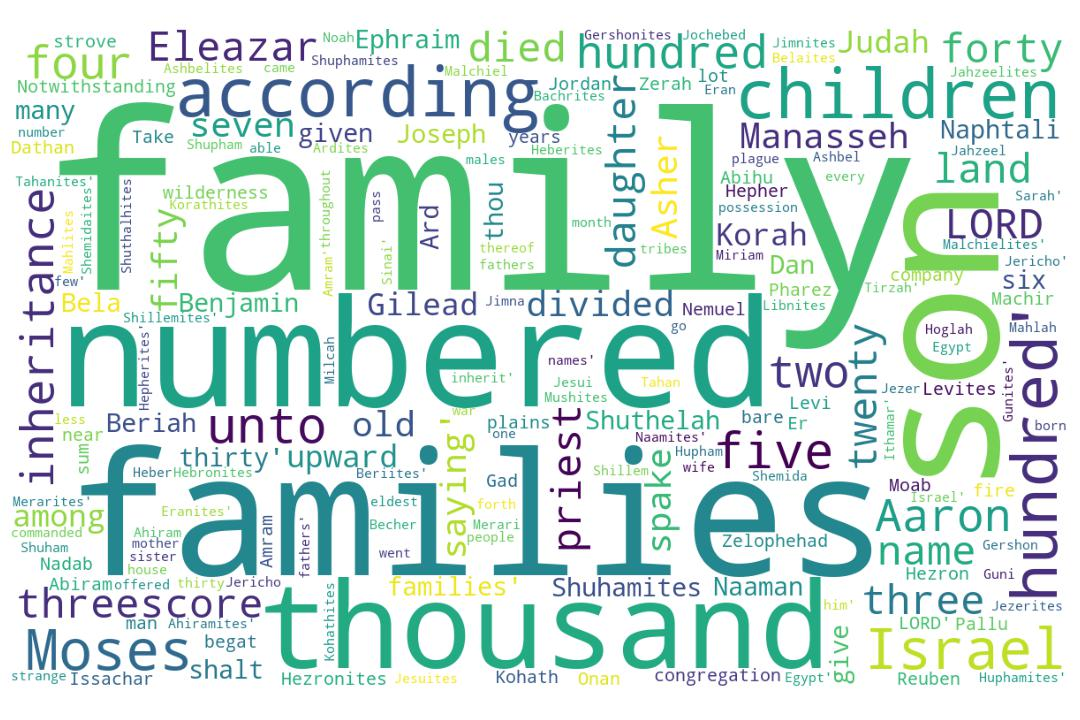
\includegraphics[width=\linewidth]{04OT-Numbers/Numbers26-WordCloud.jpg}
  \caption{Numbers 26 Word Cloud}
  \label{fig:Numbers 26 word Cloud}
\end{figure}

\marginpar{\scriptsize \centering \fcolorbox{bone}{lime}{\textbf{A GENERATION LATER}}\\ (Numbers 26)
\begin{compactenum}[I.][8]
    \item The \textbf{Priests} \index[scripture]{Numbers!Num 26:01}\index[scripture]{Numbers!Num 26:03}\index[scripture]{Numbers!Num 26:63}\index[scripture]{Numbers!Num 26:64} (Numbers 26:1, 3, 63, 64)
    \item The \textbf{Plague} \index[scripture]{Numbers!Num 26:01} (Numbers 26:1)
    \item The \textbf{Plains} of Moab \index[scripture]{Numbers!Num 26:03}\index[scripture]{Numbers!Num 26:64} (Numbers 26:3, 64)
    \item The \textbf{People} 
    \item The \textbf{Population} \index[scripture]{Numbers!Num 26:12--54} (Numbers 26:12--54) Note the differences in population among the various tribes. Simeon loses almost 63\% of its people, while some of the tribes grow substantially.
    \item The \textbf{Possessions} \index[scripture]{Numbers!Num 26:56} (Numbers 26:56)
    \item A \textbf{Preview} 
\end{compactenum}}

%%%%%%%%%%%%%%%%%%%%%%%%%%%%%%%%%%
%%%%%%%%%%%%%%%%%%%%%%%%%%%%%%%%%%
\footnote{\textcolor[rgb]{0.00,0.25,0.00}{\hyperlink{TOC}{Return to end of Table of Contents.}}}\footnote{\href{https://audiobible.com/bible/numbers_26.html}{\textcolor[cmyk]{0.99998,1,0,0}{Numbers 26 Audio}}}\textcolor[cmyk]{0.99998,1,0,0}{And it came to pass after the plague, that the LORD spake unto Moses and unto Eleazar the son of Aaron the priest, saying,}
[2] \textcolor[cmyk]{0.99998,1,0,0}{Take the sum of all the congregation of the children of Israel, from twenty years old and upward, throughout their fathers' house, all that are able to go to war in Israel.}
[3] \textcolor[cmyk]{0.99998,1,0,0}{And Moses and Eleazar the priest spake with them in the plains of Moab by Jordan \emph{near} Jericho, saying,}
[4] \textcolor[cmyk]{0.99998,1,0,0}{\emph{Take} \emph{the} \emph{sum} \emph{of} \emph{the} \emph{people}, from twenty years old and upward; as the LORD commanded Moses and the children of Israel, which went forth out of the land of Egypt.}\\
\\
\P \textcolor[cmyk]{0.99998,1,0,0}{Reuben, the eldest son of Israel: the children of Reuben; Hanoch, \emph{of} \emph{whom} \emph{cometh} the family of the Hanochites: of Pallu, the family of the Palluites:}
[6] \textcolor[cmyk]{0.99998,1,0,0}{Of Hezron, the family of the Hezronites: of Carmi, the family of the Carmites.}
[7] \textcolor[cmyk]{0.99998,1,0,0}{These \emph{are} \fcolorbox{bone}{bone}{the familes} of the Reubenites: and they that were numbered of them were forty and three \fcolorbox{bone}{bone}{thousand and} seven hundred and thirty.}
[8] \textcolor[cmyk]{0.99998,1,0,0}{And the sons of Pallu; Eliab.}
[9] \textcolor[cmyk]{0.99998,1,0,0}{And the sons of Eliab; Nemuel, and Dathan, and Abiram. This \emph{is} \emph{that} Dathan and Abiram, \emph{which} \emph{were} famous in the congregation, who strove against Moses and against Aaron in the company of Korah, when they strove against the LORD:}\footnote{\textbf{Numbers 16:1-3} - Now Korah, the son of Izhar, the son of Kohath, the son of Levi, and Dathan and Abiram, the sons of Eliab, and On, the son of Peleth, sons of Reuben, took men: [2] And they rose up before Moses, with certain of the children of Israel, two hundred and fifty princes of the assembly, famous in the congregation, men of renown: [3] And they gathered themselves together against Moses and against Aaron, and said unto them, Ye take too much upon you, seeing all the congregation are holy, every one of them, and the LORD is among them: wherefore then lift ye up yourselves above the congregation of the LORD?}\footnote{\textbf{Deuteronomy 11:6} - And what he did unto Dathan and Abiram, the sons of Eliab, the son of Reuben: how the earth opened her mouth, and swallowed them up, and their households, and their tents, and all the substance that was in their possession, in the midst of all Israel:}\footnote{\textbf{Psalm 106:17} - The earth opened and swallowed up Dathan, and covered the company of Abiram.}
[10] \textcolor[cmyk]{0.99998,1,0,0}{And the earth opened her mouth, and swallowed them up together with Korah, when that company died, what time the fire devoured two hundred and fifty men: and they became a sign.}
[11] \textcolor[cmyk]{0.99998,1,0,0}{Notwithstanding the children of Korah died not.}\\
\\
\P \textcolor[cmyk]{0.99998,1,0,0}{The sons of Simeon after their families: of Nemuel, the family of the Nemuelites: of Jamin, the family of the Jaminites: of Jachin, the family of the Jachinites:}
[13] \textcolor[cmyk]{0.99998,1,0,0}{Of Zerah, the family of the Zarhites: of Shaul, the family of the Shaulites.}
[14] \textcolor[cmyk]{0.99998,1,0,0}{These \emph{are} \fcolorbox{bone}{bone}{the familes} of the Simeonites, twenty and two \fcolorbox{bone}{bone}{thousand and} two hundred.}\\
\\
\P \textcolor[cmyk]{0.99998,1,0,0}{The children of Gad after their families: of Zephon, the family of the Zephonites: of Haggi, the family of the Haggites: of Shuni, the family of the Shunites:}
[16] \textcolor[cmyk]{0.99998,1,0,0}{Of Ozni, the family of the Oznites: of Eri, the family of the Erites:}
[17] \textcolor[cmyk]{0.99998,1,0,0}{Of Arod, the family of the Arodites: of Areli, the family of the Arelites.}
[18] \textcolor[cmyk]{0.99998,1,0,0}{These \emph{are} \fcolorbox{bone}{bone}{the familes} of the children of Gad according to those that were numbered of them, forty \fcolorbox{bone}{bone}{thousand and} five hundred.}\\
\\
\P \textcolor[cmyk]{0.99998,1,0,0}{The sons of Judah \emph{were} Er and Onan: and Er and Onan died in the land of Canaan.}
[20] \textcolor[cmyk]{0.99998,1,0,0}{And the sons of Judah after their families were; of Shelah, the family of the Shelanites: of Pharez, the family of the Pharzites: of Zerah, the family of the Zarhites.}
[21] \textcolor[cmyk]{0.99998,1,0,0}{And the sons of Pharez were; of Hezron, the family of the Hezronites: of Hamul, the family of the Hamulites.}
[22] \textcolor[cmyk]{0.99998,1,0,0}{These \emph{are} \fcolorbox{bone}{bone}{the familes} of Judah according to those that were numbered of them, threescore and sixteen \fcolorbox{bone}{bone}{thousand and} five hundred.}\\
\\
\P \textcolor[cmyk]{0.99998,1,0,0}{\emph{Of} the sons of Issachar after their families: \emph{of} Tola, the family of the Tolaites: of Pua, the family of the Punites:}
[24] \textcolor[cmyk]{0.99998,1,0,0}{Of Jashub, the family of the Jashubites: of Shimron, the family of the Shimronites.}
[25] \textcolor[cmyk]{0.99998,1,0,0}{These \emph{are} \fcolorbox{bone}{bone}{the familes} of Issachar according to those that were numbered of them, threescore and four \fcolorbox{bone}{bone}{thousand and} three hundred.}\\
\\
\P \textcolor[cmyk]{0.99998,1,0,0}{\emph{Of} the sons of Zebulun after their families: of Sered, the family of the Sardites: of Elon, the family of the Elonites: of Jahleel, the family of the Jahleelites.}
[27] \textcolor[cmyk]{0.99998,1,0,0}{These \emph{are} \fcolorbox{bone}{bone}{the familes} of the Zebulunites according to those that were numbered of them, threescore \fcolorbox{bone}{bone}{thousand and} five hundred.}\\
\\
\P \textcolor[cmyk]{0.99998,1,0,0}{The sons of Joseph after their families \emph{were} Manasseh and Ephraim.}
[29] \textcolor[cmyk]{0.99998,1,0,0}{Of the sons of Manasseh: of Machir, the family of the Machirites: and Machir begat Gilead: of Gilead \emph{come} the family of the Gileadites.}
[30] \textcolor[cmyk]{0.99998,1,0,0}{These \emph{are} the sons of Gilead: \emph{of} Jeezer, the family of the Jeezerites: of Helek, the family of the Helekites:}
[31] \textcolor[cmyk]{0.99998,1,0,0}{And \emph{of} Asriel, the family of the Asrielites: and \emph{of} Shechem, the family of the Shechemites:}
[32] \textcolor[cmyk]{0.99998,1,0,0}{And \emph{of} Shemida, the family of the Shemidaites: and \emph{of} Hepher, the family of the Hepherites.}
[33] \textcolor[cmyk]{0.99998,1,0,0}{And Zelophehad the son of Hepher had no sons, but daughters: and the names of the daughters of Zelophehad \emph{were} Mahlah, and Noah, Hoglah, Milcah, and Tirzah.}
[34] \textcolor[cmyk]{0.99998,1,0,0}{These \emph{are} \fcolorbox{bone}{bone}{the familes} of Manasseh, and those that were numbered of them, fifty and two \fcolorbox{bone}{bone}{thousand and} seven hundred.}\\
\\
\P \textcolor[cmyk]{0.99998,1,0,0}{These \emph{are} the sons of Ephraim after their families: of Shuthelah, the family of the Shuthalhites: of Becher, the family of the Bachrites: of Tahan, the family of the Tahanites.}
[36] \textcolor[cmyk]{0.99998,1,0,0}{And these \emph{are} the sons of Shuthelah: of Eran, the family of the Eranites.}
[37] \textcolor[cmyk]{0.99998,1,0,0}{These \emph{are} \fcolorbox{bone}{bone}{the familes} of the sons of Ephraim according to those that were numbered of them, thirty and two \fcolorbox{bone}{bone}{thousand and} five hundred. These \emph{are} the sons of Joseph after their families.}\\
\\
\P \textcolor[cmyk]{0.99998,1,0,0}{The sons of Benjamin after their families: of Bela, the family of the Belaites: of Ashbel, the family of the Ashbelites: of Ahiram, the family of the Ahiramites:}
[39] \textcolor[cmyk]{0.99998,1,0,0}{Of Shupham, the family of the Shuphamites: of Hupham, the family of the Huphamites.}
[40] \textcolor[cmyk]{0.99998,1,0,0}{And the sons of Bela were Ard and Naaman: \emph{of} \emph{Ard}, the family of the Ardites: \emph{and} of Naaman, the family of the Naamites.}
[41] \textcolor[cmyk]{0.99998,1,0,0}{These \emph{are} the sons of Benjamin after their families: and they that were numbered of them \emph{were} forty and five \fcolorbox{bone}{bone}{thousand and} six hundred.}\\
\\
\P \textcolor[cmyk]{0.99998,1,0,0}{These \emph{are} the sons of Dan after their families: of Shuham, the family of the Shuhamites. These \emph{are} \fcolorbox{bone}{bone}{the familes} of Dan after their families.}
[43] \textcolor[cmyk]{0.99998,1,0,0}{All \fcolorbox{bone}{bone}{the familes} of the Shuhamites, according to those that were numbered of them, \emph{were} threescore and four \fcolorbox{bone}{bone}{thousand and} four hundred.}\\
\\
\P \textcolor[cmyk]{0.99998,1,0,0}{\emph{Of} the children of Asher after their families: of Jimna, the family of the Jimnites: of Jesui, the family of the Jesuites: of Beriah, the family of the Beriites.}
[45] \textcolor[cmyk]{0.99998,1,0,0}{Of the sons of Beriah: of Heber, the family of the Heberites: of Malchiel, the family of the Malchielites.}
[46] \textcolor[cmyk]{0.99998,1,0,0}{And the name of the daughter of Asher \emph{was} Sarah.}
[47] \textcolor[cmyk]{0.99998,1,0,0}{These \emph{are} \fcolorbox{bone}{bone}{the familes} of the sons of Asher according to those that were numbered of them; \emph{who} \emph{were} fifty and three \fcolorbox{bone}{bone}{thousand and} four hundred.}\\
\\
\P \textcolor[cmyk]{0.99998,1,0,0}{\emph{Of} the sons of Naphtali after their families: of Jahzeel, the family of the Jahzeelites: of Guni, the family of the Gunites:}
[49] \textcolor[cmyk]{0.99998,1,0,0}{Of Jezer, the family of the Jezerites: of Shillem, the family of the Shillemites.}
[50] \textcolor[cmyk]{0.99998,1,0,0}{These \emph{are} \fcolorbox{bone}{bone}{the familes} of Naphtali according to their families: and they that were numbered of them \emph{were} forty and five \fcolorbox{bone}{bone}{thousand and} four hundred.}
[51] \textcolor[cmyk]{0.99998,1,0,0}{These \emph{were} the numbered of the children of Israel, six hundred \fcolorbox{bone}{bone}{thousand and} a thousand seven hundred and thirty.}\\
\\
\P \textcolor[cmyk]{0.99998,1,0,0}{And the LORD spake unto Moses, saying,}
[53] \textcolor[cmyk]{0.99998,1,0,0}{Unto these the land shall be divided for an inheritance according to the number of names.}
[54] \textcolor[cmyk]{0.99998,1,0,0}{To many thou shalt give the more inheritance, and to few thou shalt give the less inheritance: to every one shall his inheritance be given according to those that were numbered of him.}
[55] \textcolor[cmyk]{0.99998,1,0,0}{Notwithstanding the land shall be divided by lot: according to the names of the tribes of their fathers they shall inherit.}
[56] \textcolor[cmyk]{0.99998,1,0,0}{According to the lot shall the possession thereof be divided between many and few.}\\
\\
\P \textcolor[cmyk]{0.99998,1,0,0}{And these \emph{are} they that were numbered of the Levites after their families: of Gershon, the family of the Gershonites: of Kohath, the family of the Kohathites: of Merari, the family of the Merarites.}
[58] \textcolor[cmyk]{0.99998,1,0,0}{These \emph{are} \fcolorbox{bone}{bone}{the familes} of the Levites: the family of the Libnites, the family of the Hebronites, the family of the Mahlites, the family of the Mushites, the family of the Korathites. And Kohath begat Amram.}
[59] \textcolor[cmyk]{0.99998,1,0,0}{And the name of Amram's wife \emph{was} Jochebed, the daughter of Levi, whom \emph{her} \emph{mother} bare to Levi in Egypt: and she bare unto Amram Aaron and Moses, and Miriam their sister.}
[60] \textcolor[cmyk]{0.99998,1,0,0}{And unto Aaron was born Nadab, and Abihu, Eleazar, and Ithamar.}
[61] \textcolor[cmyk]{0.99998,1,0,0}{And Nadab and Abihu died, when they offered strange fire before the LORD.}\footnote{\textbf{Numbers 3:4} - And Nadab and Abihu died before the LORD, when they offered strange fire before the LORD, in the wilderness of Sinai, and they had no children: and Eleazar and Ithamar ministered in the priest’s office in the sight of Aaron their father.}\footnote{\textbf{Numbers 10:1-2} - And Nadab and Abihu, the sons of Aaron, took either of them his censer, and put fire therein, and put incense thereon, and offered strange fire before the LORD, which he commanded them not. [2] And there went out fire from the LORD, and devoured them, and they died before the LORD.}
[62] \textcolor[cmyk]{0.99998,1,0,0}{And those that were numbered of them were twenty and three thousand, all males from a month old and upward: for they were not numbered among the children of Israel, because there was no inheritance given them among the children of Israel.}
[63] \textcolor[cmyk]{0.99998,1,0,0}{These \emph{are} they that were numbered by Moses and Eleazar the priest, who numbered the children of Israel in the plains of Moab by Jordan \emph{near} Jericho.}
[64] \textcolor[cmyk]{0.99998,1,0,0}{But among these there was not a man of them whom Moses and Aaron the priest numbered, when they numbered the children of Israel in the wilderness of Sinai.}
[65] \textcolor[cmyk]{0.99998,1,0,0}{For the LORD had said of them, They shall surely die in the wilderness. And there was not left a man of them, save Caleb the son of Jephunneh, and Joshua the son of Nun.}
\index[NWIV]{24!Numbers!Num 26:1}\index[AWIP]{And!Numbers!Num 26:1}\index[AWIP]{it!Numbers!Num 26:1}\index[AWIP]{came!Numbers!Num 26:1}\index[AWIP]{to!Numbers!Num 26:1}\index[AWIP]{pass!Numbers!Num 26:1}\index[AWIP]{after!Numbers!Num 26:1}\index[AWIP]{the!Numbers!Num 26:1}\index[AWIP]{the!Numbers!Num 26:1 (2)}\index[AWIP]{the!Numbers!Num 26:1 (3)}\index[AWIP]{the!Numbers!Num 26:1 (4)}\index[AWIP]{plague!Numbers!Num 26:1}\index[AWIP]{that!Numbers!Num 26:1}\index[AWIP]{LORD!Numbers!Num 26:1}\index[AWIP]{spake!Numbers!Num 26:1}\index[AWIP]{unto!Numbers!Num 26:1}\index[AWIP]{unto!Numbers!Num 26:1 (2)}\index[AWIP]{Moses!Numbers!Num 26:1}\index[AWIP]{and!Numbers!Num 26:1}\index[AWIP]{Eleazar!Numbers!Num 26:1}\index[AWIP]{son!Numbers!Num 26:1}\index[AWIP]{of!Numbers!Num 26:1}\index[AWIP]{Aaron!Numbers!Num 26:1}\index[AWIP]{priest!Numbers!Num 26:1}\index[AWIP]{saying!Numbers!Num 26:1}

\index[NWIV]{32!Numbers!Num 26:2}\index[AWIP]{Take!Numbers!Num 26:2}\index[AWIP]{the!Numbers!Num 26:2}\index[AWIP]{the!Numbers!Num 26:2 (2)}\index[AWIP]{the!Numbers!Num 26:2 (3)}\index[AWIP]{sum!Numbers!Num 26:2}\index[AWIP]{of!Numbers!Num 26:2}\index[AWIP]{of!Numbers!Num 26:2 (2)}\index[AWIP]{of!Numbers!Num 26:2 (3)}\index[AWIP]{all!Numbers!Num 26:2}\index[AWIP]{all!Numbers!Num 26:2 (2)}\index[AWIP]{congregation!Numbers!Num 26:2}\index[AWIP]{children!Numbers!Num 26:2}\index[AWIP]{Israel!Numbers!Num 26:2}\index[AWIP]{Israel!Numbers!Num 26:2 (2)}\index[AWIP]{from!Numbers!Num 26:2}\index[AWIP]{twenty!Numbers!Num 26:2}\index[AWIP]{years!Numbers!Num 26:2}\index[AWIP]{old!Numbers!Num 26:2}\index[AWIP]{and!Numbers!Num 26:2}\index[AWIP]{upward!Numbers!Num 26:2}\index[AWIP]{throughout!Numbers!Num 26:2}\index[AWIP]{their!Numbers!Num 26:2}\index[AWIP]{fathers'!Numbers!Num 26:2}\index[AWIP]{house!Numbers!Num 26:2}\index[AWIP]{that!Numbers!Num 26:2}\index[AWIP]{are!Numbers!Num 26:2}\index[AWIP]{able!Numbers!Num 26:2}\index[AWIP]{to!Numbers!Num 26:2}\index[AWIP]{to!Numbers!Num 26:2 (2)}\index[AWIP]{go!Numbers!Num 26:2}\index[AWIP]{war!Numbers!Num 26:2}\index[AWIP]{in!Numbers!Num 26:2}

\index[NWIV]{19!Numbers!Num 26:3}\index[AWIP]{And!Numbers!Num 26:3}\index[AWIP]{Moses!Numbers!Num 26:3}\index[AWIP]{and!Numbers!Num 26:3}\index[AWIP]{Eleazar!Numbers!Num 26:3}\index[AWIP]{the!Numbers!Num 26:3}\index[AWIP]{the!Numbers!Num 26:3 (2)}\index[AWIP]{priest!Numbers!Num 26:3}\index[AWIP]{spake!Numbers!Num 26:3}\index[AWIP]{with!Numbers!Num 26:3}\index[AWIP]{them!Numbers!Num 26:3}\index[AWIP]{in!Numbers!Num 26:3}\index[AWIP]{plains!Numbers!Num 26:3}\index[AWIP]{of!Numbers!Num 26:3}\index[AWIP]{Moab!Numbers!Num 26:3}\index[AWIP]{by!Numbers!Num 26:3}\index[AWIP]{Jordan!Numbers!Num 26:3}\index[AWIP]{\emph{near}!Numbers!Num 26:3}\index[AWIP]{Jericho!Numbers!Num 26:3}\index[AWIP]{saying!Numbers!Num 26:3}\index[AWIP]{\emph{near}!Numbers!Num 26:3}

\index[NWIV]{31!Numbers!Num 26:4}\index[AWIP]{\emph{Take}!Numbers!Num 26:4}\index[AWIP]{\emph{the}!Numbers!Num 26:4}\index[AWIP]{\emph{the}!Numbers!Num 26:4 (2)}\index[AWIP]{\emph{sum}!Numbers!Num 26:4}\index[AWIP]{\emph{of}!Numbers!Num 26:4}\index[AWIP]{\emph{people}!Numbers!Num 26:4}\index[AWIP]{from!Numbers!Num 26:4}\index[AWIP]{twenty!Numbers!Num 26:4}\index[AWIP]{years!Numbers!Num 26:4}\index[AWIP]{old!Numbers!Num 26:4}\index[AWIP]{and!Numbers!Num 26:4}\index[AWIP]{and!Numbers!Num 26:4 (2)}\index[AWIP]{upward!Numbers!Num 26:4}\index[AWIP]{as!Numbers!Num 26:4}\index[AWIP]{the!Numbers!Num 26:4}\index[AWIP]{the!Numbers!Num 26:4 (2)}\index[AWIP]{the!Numbers!Num 26:4 (3)}\index[AWIP]{LORD!Numbers!Num 26:4}\index[AWIP]{commanded!Numbers!Num 26:4}\index[AWIP]{Moses!Numbers!Num 26:4}\index[AWIP]{children!Numbers!Num 26:4}\index[AWIP]{of!Numbers!Num 26:4}\index[AWIP]{of!Numbers!Num 26:4 (2)}\index[AWIP]{of!Numbers!Num 26:4 (3)}\index[AWIP]{Israel!Numbers!Num 26:4}\index[AWIP]{which!Numbers!Num 26:4}\index[AWIP]{went!Numbers!Num 26:4}\index[AWIP]{forth!Numbers!Num 26:4}\index[AWIP]{out!Numbers!Num 26:4}\index[AWIP]{land!Numbers!Num 26:4}\index[AWIP]{Egypt!Numbers!Num 26:4}\index[AWIP]{\emph{Take}!Numbers!Num 26:4}\index[AWIP]{\emph{the}!Numbers!Num 26:4}\index[AWIP]{\emph{the}!Numbers!Num 26:4 (2)}\index[AWIP]{\emph{sum}!Numbers!Num 26:4}\index[AWIP]{\emph{of}!Numbers!Num 26:4}\index[AWIP]{\emph{people}!Numbers!Num 26:4}

\index[NWIV]{26!Numbers!Num 26:5}\index[AWIP]{Reuben!Numbers!Num 26:5}\index[AWIP]{Reuben!Numbers!Num 26:5 (2)}\index[AWIP]{the!Numbers!Num 26:5}\index[AWIP]{the!Numbers!Num 26:5 (2)}\index[AWIP]{the!Numbers!Num 26:5 (3)}\index[AWIP]{the!Numbers!Num 26:5 (4)}\index[AWIP]{the!Numbers!Num 26:5 (5)}\index[AWIP]{the!Numbers!Num 26:5 (6)}\index[AWIP]{eldest!Numbers!Num 26:5}\index[AWIP]{son!Numbers!Num 26:5}\index[AWIP]{of!Numbers!Num 26:5}\index[AWIP]{of!Numbers!Num 26:5 (2)}\index[AWIP]{of!Numbers!Num 26:5 (3)}\index[AWIP]{of!Numbers!Num 26:5 (4)}\index[AWIP]{of!Numbers!Num 26:5 (5)}\index[AWIP]{Israel!Numbers!Num 26:5}\index[AWIP]{children!Numbers!Num 26:5}\index[AWIP]{Hanoch!Numbers!Num 26:5}\index[AWIP]{\emph{of}!Numbers!Num 26:5}\index[AWIP]{\emph{whom}!Numbers!Num 26:5}\index[AWIP]{\emph{cometh}!Numbers!Num 26:5}\index[AWIP]{family!Numbers!Num 26:5}\index[AWIP]{family!Numbers!Num 26:5 (2)}\index[AWIP]{Hanochites!Numbers!Num 26:5}\index[AWIP]{Pallu!Numbers!Num 26:5}\index[AWIP]{Palluites!Numbers!Num 26:5}\index[AWIP]{\emph{of}!Numbers!Num 26:5}\index[AWIP]{\emph{whom}!Numbers!Num 26:5}\index[AWIP]{\emph{cometh}!Numbers!Num 26:5}

\index[NWIV]{14!Numbers!Num 26:6}\index[AWIP]{Of!Numbers!Num 26:6}\index[AWIP]{Hezron!Numbers!Num 26:6}\index[AWIP]{the!Numbers!Num 26:6}\index[AWIP]{the!Numbers!Num 26:6 (2)}\index[AWIP]{the!Numbers!Num 26:6 (3)}\index[AWIP]{the!Numbers!Num 26:6 (4)}\index[AWIP]{family!Numbers!Num 26:6}\index[AWIP]{family!Numbers!Num 26:6 (2)}\index[AWIP]{of!Numbers!Num 26:6}\index[AWIP]{of!Numbers!Num 26:6 (2)}\index[AWIP]{of!Numbers!Num 26:6 (3)}\index[AWIP]{Hezronites!Numbers!Num 26:6}\index[AWIP]{Carmi!Numbers!Num 26:6}\index[AWIP]{Carmites!Numbers!Num 26:6}

\index[NWIV]{24!Numbers!Num 26:7}\index[AWIP]{These!Numbers!Num 26:7}\index[AWIP]{\emph{are}!Numbers!Num 26:7}\index[AWIP]{the!Numbers!Num 26:7}\index[AWIP]{the!Numbers!Num 26:7 (2)}\index[AWIP]{families!Numbers!Num 26:7}\index[AWIP]{of!Numbers!Num 26:7}\index[AWIP]{of!Numbers!Num 26:7 (2)}\index[AWIP]{Reubenites!Numbers!Num 26:7}\index[AWIP]{and!Numbers!Num 26:7}\index[AWIP]{and!Numbers!Num 26:7 (2)}\index[AWIP]{and!Numbers!Num 26:7 (3)}\index[AWIP]{and!Numbers!Num 26:7 (4)}\index[AWIP]{they!Numbers!Num 26:7}\index[AWIP]{that!Numbers!Num 26:7}\index[AWIP]{were!Numbers!Num 26:7}\index[AWIP]{were!Numbers!Num 26:7 (2)}\index[AWIP]{numbered!Numbers!Num 26:7}\index[AWIP]{them!Numbers!Num 26:7}\index[AWIP]{forty!Numbers!Num 26:7}\index[AWIP]{three!Numbers!Num 26:7}\index[AWIP]{thousand!Numbers!Num 26:7}\index[AWIP]{seven!Numbers!Num 26:7}\index[AWIP]{hundred!Numbers!Num 26:7}\index[AWIP]{thirty!Numbers!Num 26:7}\index[AWIP]{\emph{are}!Numbers!Num 26:7}

\index[NWIV]{6!Numbers!Num 26:8}\index[AWIP]{And!Numbers!Num 26:8}\index[AWIP]{the!Numbers!Num 26:8}\index[AWIP]{sons!Numbers!Num 26:8}\index[AWIP]{of!Numbers!Num 26:8}\index[AWIP]{Pallu!Numbers!Num 26:8}\index[AWIP]{Eliab!Numbers!Num 26:8}

\index[NWIV]{40!Numbers!Num 26:9}\index[AWIP]{And!Numbers!Num 26:9}\index[AWIP]{the!Numbers!Num 26:9}\index[AWIP]{the!Numbers!Num 26:9 (2)}\index[AWIP]{the!Numbers!Num 26:9 (3)}\index[AWIP]{the!Numbers!Num 26:9 (4)}\index[AWIP]{sons!Numbers!Num 26:9}\index[AWIP]{of!Numbers!Num 26:9}\index[AWIP]{of!Numbers!Num 26:9 (2)}\index[AWIP]{Eliab!Numbers!Num 26:9}\index[AWIP]{Nemuel!Numbers!Num 26:9}\index[AWIP]{and!Numbers!Num 26:9}\index[AWIP]{and!Numbers!Num 26:9 (2)}\index[AWIP]{and!Numbers!Num 26:9 (3)}\index[AWIP]{and!Numbers!Num 26:9 (4)}\index[AWIP]{Dathan!Numbers!Num 26:9}\index[AWIP]{Dathan!Numbers!Num 26:9 (2)}\index[AWIP]{Abiram!Numbers!Num 26:9}\index[AWIP]{Abiram!Numbers!Num 26:9 (2)}\index[AWIP]{This!Numbers!Num 26:9}\index[AWIP]{\emph{is}!Numbers!Num 26:9}\index[AWIP]{\emph{that}!Numbers!Num 26:9}\index[AWIP]{\emph{which}!Numbers!Num 26:9}\index[AWIP]{\emph{were}!Numbers!Num 26:9}\index[AWIP]{famous!Numbers!Num 26:9}\index[AWIP]{in!Numbers!Num 26:9}\index[AWIP]{in!Numbers!Num 26:9 (2)}\index[AWIP]{congregation!Numbers!Num 26:9}\index[AWIP]{who!Numbers!Num 26:9}\index[AWIP]{strove!Numbers!Num 26:9}\index[AWIP]{strove!Numbers!Num 26:9 (2)}\index[AWIP]{against!Numbers!Num 26:9}\index[AWIP]{against!Numbers!Num 26:9 (2)}\index[AWIP]{against!Numbers!Num 26:9 (3)}\index[AWIP]{Moses!Numbers!Num 26:9}\index[AWIP]{Aaron!Numbers!Num 26:9}\index[AWIP]{company!Numbers!Num 26:9}\index[AWIP]{Korah!Numbers!Num 26:9}\index[AWIP]{when!Numbers!Num 26:9}\index[AWIP]{they!Numbers!Num 26:9}\index[AWIP]{LORD!Numbers!Num 26:9}\index[AWIP]{\emph{is}!Numbers!Num 26:9}\index[AWIP]{\emph{that}!Numbers!Num 26:9}\index[AWIP]{\emph{which}!Numbers!Num 26:9}\index[AWIP]{\emph{were}!Numbers!Num 26:9}

\index[NWIV]{32!Numbers!Num 26:10}\index[AWIP]{And!Numbers!Num 26:10}\index[AWIP]{the!Numbers!Num 26:10}\index[AWIP]{the!Numbers!Num 26:10 (2)}\index[AWIP]{earth!Numbers!Num 26:10}\index[AWIP]{opened!Numbers!Num 26:10}\index[AWIP]{her!Numbers!Num 26:10}\index[AWIP]{mouth!Numbers!Num 26:10}\index[AWIP]{and!Numbers!Num 26:10}\index[AWIP]{and!Numbers!Num 26:10 (2)}\index[AWIP]{and!Numbers!Num 26:10 (3)}\index[AWIP]{swallowed!Numbers!Num 26:10}\index[AWIP]{them!Numbers!Num 26:10}\index[AWIP]{up!Numbers!Num 26:10}\index[AWIP]{together!Numbers!Num 26:10}\index[AWIP]{with!Numbers!Num 26:10}\index[AWIP]{Korah!Numbers!Num 26:10}\index[AWIP]{when!Numbers!Num 26:10}\index[AWIP]{that!Numbers!Num 26:10}\index[AWIP]{company!Numbers!Num 26:10}\index[AWIP]{died!Numbers!Num 26:10}\index[AWIP]{what!Numbers!Num 26:10}\index[AWIP]{time!Numbers!Num 26:10}\index[AWIP]{fire!Numbers!Num 26:10}\index[AWIP]{devoured!Numbers!Num 26:10}\index[AWIP]{two!Numbers!Num 26:10}\index[AWIP]{hundred!Numbers!Num 26:10}\index[AWIP]{fifty!Numbers!Num 26:10}\index[AWIP]{men!Numbers!Num 26:10}\index[AWIP]{they!Numbers!Num 26:10}\index[AWIP]{became!Numbers!Num 26:10}\index[AWIP]{a!Numbers!Num 26:10}\index[AWIP]{sign!Numbers!Num 26:10}

\index[NWIV]{7!Numbers!Num 26:11}\index[AWIP]{Notwithstanding!Numbers!Num 26:11}\index[AWIP]{the!Numbers!Num 26:11}\index[AWIP]{children!Numbers!Num 26:11}\index[AWIP]{of!Numbers!Num 26:11}\index[AWIP]{Korah!Numbers!Num 26:11}\index[AWIP]{died!Numbers!Num 26:11}\index[AWIP]{not!Numbers!Num 26:11}

\index[NWIV]{28!Numbers!Num 26:12}\index[AWIP]{The!Numbers!Num 26:12}\index[AWIP]{sons!Numbers!Num 26:12}\index[AWIP]{of!Numbers!Num 26:12}\index[AWIP]{of!Numbers!Num 26:12 (2)}\index[AWIP]{of!Numbers!Num 26:12 (3)}\index[AWIP]{of!Numbers!Num 26:12 (4)}\index[AWIP]{of!Numbers!Num 26:12 (5)}\index[AWIP]{of!Numbers!Num 26:12 (6)}\index[AWIP]{of!Numbers!Num 26:12 (7)}\index[AWIP]{Simeon!Numbers!Num 26:12}\index[AWIP]{after!Numbers!Num 26:12}\index[AWIP]{their!Numbers!Num 26:12}\index[AWIP]{families!Numbers!Num 26:12}\index[AWIP]{Nemuel!Numbers!Num 26:12}\index[AWIP]{the!Numbers!Num 26:12}\index[AWIP]{the!Numbers!Num 26:12 (2)}\index[AWIP]{the!Numbers!Num 26:12 (3)}\index[AWIP]{the!Numbers!Num 26:12 (4)}\index[AWIP]{the!Numbers!Num 26:12 (5)}\index[AWIP]{the!Numbers!Num 26:12 (6)}\index[AWIP]{family!Numbers!Num 26:12}\index[AWIP]{family!Numbers!Num 26:12 (2)}\index[AWIP]{family!Numbers!Num 26:12 (3)}\index[AWIP]{Nemuelites!Numbers!Num 26:12}\index[AWIP]{Jamin!Numbers!Num 26:12}\index[AWIP]{Jaminites!Numbers!Num 26:12}\index[AWIP]{Jachin!Numbers!Num 26:12}\index[AWIP]{Jachinites!Numbers!Num 26:12}

\index[NWIV]{14!Numbers!Num 26:13}\index[AWIP]{Of!Numbers!Num 26:13}\index[AWIP]{Zerah!Numbers!Num 26:13}\index[AWIP]{the!Numbers!Num 26:13}\index[AWIP]{the!Numbers!Num 26:13 (2)}\index[AWIP]{the!Numbers!Num 26:13 (3)}\index[AWIP]{the!Numbers!Num 26:13 (4)}\index[AWIP]{family!Numbers!Num 26:13}\index[AWIP]{family!Numbers!Num 26:13 (2)}\index[AWIP]{of!Numbers!Num 26:13}\index[AWIP]{of!Numbers!Num 26:13 (2)}\index[AWIP]{of!Numbers!Num 26:13 (3)}\index[AWIP]{Zarhites!Numbers!Num 26:13}\index[AWIP]{Shaul!Numbers!Num 26:13}\index[AWIP]{Shaulites!Numbers!Num 26:13}

\index[NWIV]{14!Numbers!Num 26:14}\index[AWIP]{These!Numbers!Num 26:14}\index[AWIP]{\emph{are}!Numbers!Num 26:14}\index[AWIP]{the!Numbers!Num 26:14}\index[AWIP]{the!Numbers!Num 26:14 (2)}\index[AWIP]{families!Numbers!Num 26:14}\index[AWIP]{of!Numbers!Num 26:14}\index[AWIP]{Simeonites!Numbers!Num 26:14}\index[AWIP]{twenty!Numbers!Num 26:14}\index[AWIP]{and!Numbers!Num 26:14}\index[AWIP]{and!Numbers!Num 26:14 (2)}\index[AWIP]{two!Numbers!Num 26:14}\index[AWIP]{two!Numbers!Num 26:14 (2)}\index[AWIP]{thousand!Numbers!Num 26:14}\index[AWIP]{hundred!Numbers!Num 26:14}\index[AWIP]{\emph{are}!Numbers!Num 26:14}

\index[NWIV]{28!Numbers!Num 26:15}\index[AWIP]{The!Numbers!Num 26:15}\index[AWIP]{children!Numbers!Num 26:15}\index[AWIP]{of!Numbers!Num 26:15}\index[AWIP]{of!Numbers!Num 26:15 (2)}\index[AWIP]{of!Numbers!Num 26:15 (3)}\index[AWIP]{of!Numbers!Num 26:15 (4)}\index[AWIP]{of!Numbers!Num 26:15 (5)}\index[AWIP]{of!Numbers!Num 26:15 (6)}\index[AWIP]{of!Numbers!Num 26:15 (7)}\index[AWIP]{Gad!Numbers!Num 26:15}\index[AWIP]{after!Numbers!Num 26:15}\index[AWIP]{their!Numbers!Num 26:15}\index[AWIP]{families!Numbers!Num 26:15}\index[AWIP]{Zephon!Numbers!Num 26:15}\index[AWIP]{the!Numbers!Num 26:15}\index[AWIP]{the!Numbers!Num 26:15 (2)}\index[AWIP]{the!Numbers!Num 26:15 (3)}\index[AWIP]{the!Numbers!Num 26:15 (4)}\index[AWIP]{the!Numbers!Num 26:15 (5)}\index[AWIP]{the!Numbers!Num 26:15 (6)}\index[AWIP]{family!Numbers!Num 26:15}\index[AWIP]{family!Numbers!Num 26:15 (2)}\index[AWIP]{family!Numbers!Num 26:15 (3)}\index[AWIP]{Zephonites!Numbers!Num 26:15}\index[AWIP]{Haggi!Numbers!Num 26:15}\index[AWIP]{Haggites!Numbers!Num 26:15}\index[AWIP]{Shuni!Numbers!Num 26:15}\index[AWIP]{Shunites!Numbers!Num 26:15}

\index[NWIV]{14!Numbers!Num 26:16}\index[AWIP]{Of!Numbers!Num 26:16}\index[AWIP]{Ozni!Numbers!Num 26:16}\index[AWIP]{the!Numbers!Num 26:16}\index[AWIP]{the!Numbers!Num 26:16 (2)}\index[AWIP]{the!Numbers!Num 26:16 (3)}\index[AWIP]{the!Numbers!Num 26:16 (4)}\index[AWIP]{family!Numbers!Num 26:16}\index[AWIP]{family!Numbers!Num 26:16 (2)}\index[AWIP]{of!Numbers!Num 26:16}\index[AWIP]{of!Numbers!Num 26:16 (2)}\index[AWIP]{of!Numbers!Num 26:16 (3)}\index[AWIP]{Oznites!Numbers!Num 26:16}\index[AWIP]{Eri!Numbers!Num 26:16}\index[AWIP]{Erites!Numbers!Num 26:16}

\index[NWIV]{14!Numbers!Num 26:17}\index[AWIP]{Of!Numbers!Num 26:17}\index[AWIP]{Arod!Numbers!Num 26:17}\index[AWIP]{the!Numbers!Num 26:17}\index[AWIP]{the!Numbers!Num 26:17 (2)}\index[AWIP]{the!Numbers!Num 26:17 (3)}\index[AWIP]{the!Numbers!Num 26:17 (4)}\index[AWIP]{family!Numbers!Num 26:17}\index[AWIP]{family!Numbers!Num 26:17 (2)}\index[AWIP]{of!Numbers!Num 26:17}\index[AWIP]{of!Numbers!Num 26:17 (2)}\index[AWIP]{of!Numbers!Num 26:17 (3)}\index[AWIP]{Arodites!Numbers!Num 26:17}\index[AWIP]{Areli!Numbers!Num 26:17}\index[AWIP]{Arelites!Numbers!Num 26:17}

\index[NWIV]{22!Numbers!Num 26:18}\index[AWIP]{These!Numbers!Num 26:18}\index[AWIP]{\emph{are}!Numbers!Num 26:18}\index[AWIP]{the!Numbers!Num 26:18}\index[AWIP]{the!Numbers!Num 26:18 (2)}\index[AWIP]{families!Numbers!Num 26:18}\index[AWIP]{of!Numbers!Num 26:18}\index[AWIP]{of!Numbers!Num 26:18 (2)}\index[AWIP]{of!Numbers!Num 26:18 (3)}\index[AWIP]{children!Numbers!Num 26:18}\index[AWIP]{Gad!Numbers!Num 26:18}\index[AWIP]{according!Numbers!Num 26:18}\index[AWIP]{to!Numbers!Num 26:18}\index[AWIP]{those!Numbers!Num 26:18}\index[AWIP]{that!Numbers!Num 26:18}\index[AWIP]{were!Numbers!Num 26:18}\index[AWIP]{numbered!Numbers!Num 26:18}\index[AWIP]{them!Numbers!Num 26:18}\index[AWIP]{forty!Numbers!Num 26:18}\index[AWIP]{thousand!Numbers!Num 26:18}\index[AWIP]{and!Numbers!Num 26:18}\index[AWIP]{five!Numbers!Num 26:18}\index[AWIP]{hundred!Numbers!Num 26:18}\index[AWIP]{\emph{are}!Numbers!Num 26:18}

\index[NWIV]{18!Numbers!Num 26:19}\index[AWIP]{The!Numbers!Num 26:19}\index[AWIP]{sons!Numbers!Num 26:19}\index[AWIP]{of!Numbers!Num 26:19}\index[AWIP]{of!Numbers!Num 26:19 (2)}\index[AWIP]{Judah!Numbers!Num 26:19}\index[AWIP]{\emph{were}!Numbers!Num 26:19}\index[AWIP]{Er!Numbers!Num 26:19}\index[AWIP]{Er!Numbers!Num 26:19 (2)}\index[AWIP]{and!Numbers!Num 26:19}\index[AWIP]{and!Numbers!Num 26:19 (2)}\index[AWIP]{and!Numbers!Num 26:19 (3)}\index[AWIP]{Onan!Numbers!Num 26:19}\index[AWIP]{Onan!Numbers!Num 26:19 (2)}\index[AWIP]{died!Numbers!Num 26:19}\index[AWIP]{in!Numbers!Num 26:19}\index[AWIP]{the!Numbers!Num 26:19}\index[AWIP]{land!Numbers!Num 26:19}\index[AWIP]{Canaan!Numbers!Num 26:19}\index[AWIP]{\emph{were}!Numbers!Num 26:19}

\index[NWIV]{30!Numbers!Num 26:20}\index[AWIP]{And!Numbers!Num 26:20}\index[AWIP]{the!Numbers!Num 26:20}\index[AWIP]{the!Numbers!Num 26:20 (2)}\index[AWIP]{the!Numbers!Num 26:20 (3)}\index[AWIP]{the!Numbers!Num 26:20 (4)}\index[AWIP]{the!Numbers!Num 26:20 (5)}\index[AWIP]{the!Numbers!Num 26:20 (6)}\index[AWIP]{the!Numbers!Num 26:20 (7)}\index[AWIP]{sons!Numbers!Num 26:20}\index[AWIP]{of!Numbers!Num 26:20}\index[AWIP]{of!Numbers!Num 26:20 (2)}\index[AWIP]{of!Numbers!Num 26:20 (3)}\index[AWIP]{of!Numbers!Num 26:20 (4)}\index[AWIP]{of!Numbers!Num 26:20 (5)}\index[AWIP]{of!Numbers!Num 26:20 (6)}\index[AWIP]{of!Numbers!Num 26:20 (7)}\index[AWIP]{Judah!Numbers!Num 26:20}\index[AWIP]{after!Numbers!Num 26:20}\index[AWIP]{their!Numbers!Num 26:20}\index[AWIP]{families!Numbers!Num 26:20}\index[AWIP]{were!Numbers!Num 26:20}\index[AWIP]{Shelah!Numbers!Num 26:20}\index[AWIP]{family!Numbers!Num 26:20}\index[AWIP]{family!Numbers!Num 26:20 (2)}\index[AWIP]{family!Numbers!Num 26:20 (3)}\index[AWIP]{Shelanites!Numbers!Num 26:20}\index[AWIP]{Pharez!Numbers!Num 26:20}\index[AWIP]{Pharzites!Numbers!Num 26:20}\index[AWIP]{Zerah!Numbers!Num 26:20}\index[AWIP]{Zarhites!Numbers!Num 26:20}

\index[NWIV]{20!Numbers!Num 26:21}\index[AWIP]{And!Numbers!Num 26:21}\index[AWIP]{the!Numbers!Num 26:21}\index[AWIP]{the!Numbers!Num 26:21 (2)}\index[AWIP]{the!Numbers!Num 26:21 (3)}\index[AWIP]{the!Numbers!Num 26:21 (4)}\index[AWIP]{the!Numbers!Num 26:21 (5)}\index[AWIP]{sons!Numbers!Num 26:21}\index[AWIP]{of!Numbers!Num 26:21}\index[AWIP]{of!Numbers!Num 26:21 (2)}\index[AWIP]{of!Numbers!Num 26:21 (3)}\index[AWIP]{of!Numbers!Num 26:21 (4)}\index[AWIP]{of!Numbers!Num 26:21 (5)}\index[AWIP]{Pharez!Numbers!Num 26:21}\index[AWIP]{were!Numbers!Num 26:21}\index[AWIP]{Hezron!Numbers!Num 26:21}\index[AWIP]{family!Numbers!Num 26:21}\index[AWIP]{family!Numbers!Num 26:21 (2)}\index[AWIP]{Hezronites!Numbers!Num 26:21}\index[AWIP]{Hamul!Numbers!Num 26:21}\index[AWIP]{Hamulites!Numbers!Num 26:21}

\index[NWIV]{21!Numbers!Num 26:22}\index[AWIP]{These!Numbers!Num 26:22}\index[AWIP]{\emph{are}!Numbers!Num 26:22}\index[AWIP]{the!Numbers!Num 26:22}\index[AWIP]{families!Numbers!Num 26:22}\index[AWIP]{of!Numbers!Num 26:22}\index[AWIP]{of!Numbers!Num 26:22 (2)}\index[AWIP]{Judah!Numbers!Num 26:22}\index[AWIP]{according!Numbers!Num 26:22}\index[AWIP]{to!Numbers!Num 26:22}\index[AWIP]{those!Numbers!Num 26:22}\index[AWIP]{that!Numbers!Num 26:22}\index[AWIP]{were!Numbers!Num 26:22}\index[AWIP]{numbered!Numbers!Num 26:22}\index[AWIP]{them!Numbers!Num 26:22}\index[AWIP]{threescore!Numbers!Num 26:22}\index[AWIP]{and!Numbers!Num 26:22}\index[AWIP]{and!Numbers!Num 26:22 (2)}\index[AWIP]{sixteen!Numbers!Num 26:22}\index[AWIP]{thousand!Numbers!Num 26:22}\index[AWIP]{five!Numbers!Num 26:22}\index[AWIP]{hundred!Numbers!Num 26:22}\index[AWIP]{\emph{are}!Numbers!Num 26:22}

\index[NWIV]{22!Numbers!Num 26:23}\index[AWIP]{\emph{Of}!Numbers!Num 26:23}\index[AWIP]{the!Numbers!Num 26:23}\index[AWIP]{the!Numbers!Num 26:23 (2)}\index[AWIP]{the!Numbers!Num 26:23 (3)}\index[AWIP]{the!Numbers!Num 26:23 (4)}\index[AWIP]{the!Numbers!Num 26:23 (5)}\index[AWIP]{sons!Numbers!Num 26:23}\index[AWIP]{of!Numbers!Num 26:23}\index[AWIP]{of!Numbers!Num 26:23 (2)}\index[AWIP]{of!Numbers!Num 26:23 (3)}\index[AWIP]{of!Numbers!Num 26:23 (4)}\index[AWIP]{Issachar!Numbers!Num 26:23}\index[AWIP]{after!Numbers!Num 26:23}\index[AWIP]{their!Numbers!Num 26:23}\index[AWIP]{families!Numbers!Num 26:23}\index[AWIP]{\emph{of}!Numbers!Num 26:23}\index[AWIP]{Tola!Numbers!Num 26:23}\index[AWIP]{family!Numbers!Num 26:23}\index[AWIP]{family!Numbers!Num 26:23 (2)}\index[AWIP]{Tolaites!Numbers!Num 26:23}\index[AWIP]{Pua!Numbers!Num 26:23}\index[AWIP]{Punites!Numbers!Num 26:23}\index[AWIP]{\emph{Of}!Numbers!Num 26:23}\index[AWIP]{\emph{of}!Numbers!Num 26:23}

\index[NWIV]{14!Numbers!Num 26:24}\index[AWIP]{Of!Numbers!Num 26:24}\index[AWIP]{Jashub!Numbers!Num 26:24}\index[AWIP]{the!Numbers!Num 26:24}\index[AWIP]{the!Numbers!Num 26:24 (2)}\index[AWIP]{the!Numbers!Num 26:24 (3)}\index[AWIP]{the!Numbers!Num 26:24 (4)}\index[AWIP]{family!Numbers!Num 26:24}\index[AWIP]{family!Numbers!Num 26:24 (2)}\index[AWIP]{of!Numbers!Num 26:24}\index[AWIP]{of!Numbers!Num 26:24 (2)}\index[AWIP]{of!Numbers!Num 26:24 (3)}\index[AWIP]{Jashubites!Numbers!Num 26:24}\index[AWIP]{Shimron!Numbers!Num 26:24}\index[AWIP]{Shimronites!Numbers!Num 26:24}

\index[NWIV]{21!Numbers!Num 26:25}\index[AWIP]{These!Numbers!Num 26:25}\index[AWIP]{\emph{are}!Numbers!Num 26:25}\index[AWIP]{the!Numbers!Num 26:25}\index[AWIP]{families!Numbers!Num 26:25}\index[AWIP]{of!Numbers!Num 26:25}\index[AWIP]{of!Numbers!Num 26:25 (2)}\index[AWIP]{Issachar!Numbers!Num 26:25}\index[AWIP]{according!Numbers!Num 26:25}\index[AWIP]{to!Numbers!Num 26:25}\index[AWIP]{those!Numbers!Num 26:25}\index[AWIP]{that!Numbers!Num 26:25}\index[AWIP]{were!Numbers!Num 26:25}\index[AWIP]{numbered!Numbers!Num 26:25}\index[AWIP]{them!Numbers!Num 26:25}\index[AWIP]{threescore!Numbers!Num 26:25}\index[AWIP]{and!Numbers!Num 26:25}\index[AWIP]{and!Numbers!Num 26:25 (2)}\index[AWIP]{four!Numbers!Num 26:25}\index[AWIP]{thousand!Numbers!Num 26:25}\index[AWIP]{three!Numbers!Num 26:25}\index[AWIP]{hundred!Numbers!Num 26:25}\index[AWIP]{\emph{are}!Numbers!Num 26:25}

\index[NWIV]{29!Numbers!Num 26:26}\index[AWIP]{\emph{Of}!Numbers!Num 26:26}\index[AWIP]{the!Numbers!Num 26:26}\index[AWIP]{the!Numbers!Num 26:26 (2)}\index[AWIP]{the!Numbers!Num 26:26 (3)}\index[AWIP]{the!Numbers!Num 26:26 (4)}\index[AWIP]{the!Numbers!Num 26:26 (5)}\index[AWIP]{the!Numbers!Num 26:26 (6)}\index[AWIP]{the!Numbers!Num 26:26 (7)}\index[AWIP]{sons!Numbers!Num 26:26}\index[AWIP]{of!Numbers!Num 26:26}\index[AWIP]{of!Numbers!Num 26:26 (2)}\index[AWIP]{of!Numbers!Num 26:26 (3)}\index[AWIP]{of!Numbers!Num 26:26 (4)}\index[AWIP]{of!Numbers!Num 26:26 (5)}\index[AWIP]{of!Numbers!Num 26:26 (6)}\index[AWIP]{of!Numbers!Num 26:26 (7)}\index[AWIP]{Zebulun!Numbers!Num 26:26}\index[AWIP]{after!Numbers!Num 26:26}\index[AWIP]{their!Numbers!Num 26:26}\index[AWIP]{families!Numbers!Num 26:26}\index[AWIP]{Sered!Numbers!Num 26:26}\index[AWIP]{family!Numbers!Num 26:26}\index[AWIP]{family!Numbers!Num 26:26 (2)}\index[AWIP]{family!Numbers!Num 26:26 (3)}\index[AWIP]{Sardites!Numbers!Num 26:26}\index[AWIP]{Elon!Numbers!Num 26:26}\index[AWIP]{Elonites!Numbers!Num 26:26}\index[AWIP]{Jahleel!Numbers!Num 26:26}\index[AWIP]{Jahleelites!Numbers!Num 26:26}\index[AWIP]{\emph{Of}!Numbers!Num 26:26}

\index[NWIV]{20!Numbers!Num 26:27}\index[AWIP]{These!Numbers!Num 26:27}\index[AWIP]{\emph{are}!Numbers!Num 26:27}\index[AWIP]{the!Numbers!Num 26:27}\index[AWIP]{the!Numbers!Num 26:27 (2)}\index[AWIP]{families!Numbers!Num 26:27}\index[AWIP]{of!Numbers!Num 26:27}\index[AWIP]{of!Numbers!Num 26:27 (2)}\index[AWIP]{Zebulunites!Numbers!Num 26:27}\index[AWIP]{according!Numbers!Num 26:27}\index[AWIP]{to!Numbers!Num 26:27}\index[AWIP]{those!Numbers!Num 26:27}\index[AWIP]{that!Numbers!Num 26:27}\index[AWIP]{were!Numbers!Num 26:27}\index[AWIP]{numbered!Numbers!Num 26:27}\index[AWIP]{them!Numbers!Num 26:27}\index[AWIP]{threescore!Numbers!Num 26:27}\index[AWIP]{thousand!Numbers!Num 26:27}\index[AWIP]{and!Numbers!Num 26:27}\index[AWIP]{five!Numbers!Num 26:27}\index[AWIP]{hundred!Numbers!Num 26:27}\index[AWIP]{\emph{are}!Numbers!Num 26:27}

\index[NWIV]{11!Numbers!Num 26:28}\index[AWIP]{The!Numbers!Num 26:28}\index[AWIP]{sons!Numbers!Num 26:28}\index[AWIP]{of!Numbers!Num 26:28}\index[AWIP]{Joseph!Numbers!Num 26:28}\index[AWIP]{after!Numbers!Num 26:28}\index[AWIP]{their!Numbers!Num 26:28}\index[AWIP]{families!Numbers!Num 26:28}\index[AWIP]{\emph{were}!Numbers!Num 26:28}\index[AWIP]{Manasseh!Numbers!Num 26:28}\index[AWIP]{and!Numbers!Num 26:28}\index[AWIP]{Ephraim!Numbers!Num 26:28}\index[AWIP]{\emph{were}!Numbers!Num 26:28}

\index[NWIV]{24!Numbers!Num 26:29}\index[AWIP]{Of!Numbers!Num 26:29}\index[AWIP]{the!Numbers!Num 26:29}\index[AWIP]{the!Numbers!Num 26:29 (2)}\index[AWIP]{the!Numbers!Num 26:29 (3)}\index[AWIP]{the!Numbers!Num 26:29 (4)}\index[AWIP]{the!Numbers!Num 26:29 (5)}\index[AWIP]{sons!Numbers!Num 26:29}\index[AWIP]{of!Numbers!Num 26:29}\index[AWIP]{of!Numbers!Num 26:29 (2)}\index[AWIP]{of!Numbers!Num 26:29 (3)}\index[AWIP]{of!Numbers!Num 26:29 (4)}\index[AWIP]{of!Numbers!Num 26:29 (5)}\index[AWIP]{Manasseh!Numbers!Num 26:29}\index[AWIP]{Machir!Numbers!Num 26:29}\index[AWIP]{Machir!Numbers!Num 26:29 (2)}\index[AWIP]{family!Numbers!Num 26:29}\index[AWIP]{family!Numbers!Num 26:29 (2)}\index[AWIP]{Machirites!Numbers!Num 26:29}\index[AWIP]{and!Numbers!Num 26:29}\index[AWIP]{begat!Numbers!Num 26:29}\index[AWIP]{Gilead!Numbers!Num 26:29}\index[AWIP]{Gilead!Numbers!Num 26:29 (2)}\index[AWIP]{\emph{come}!Numbers!Num 26:29}\index[AWIP]{Gileadites!Numbers!Num 26:29}\index[AWIP]{\emph{come}!Numbers!Num 26:29}

\index[NWIV]{20!Numbers!Num 26:30}\index[AWIP]{These!Numbers!Num 26:30}\index[AWIP]{\emph{are}!Numbers!Num 26:30}\index[AWIP]{the!Numbers!Num 26:30}\index[AWIP]{the!Numbers!Num 26:30 (2)}\index[AWIP]{the!Numbers!Num 26:30 (3)}\index[AWIP]{the!Numbers!Num 26:30 (4)}\index[AWIP]{the!Numbers!Num 26:30 (5)}\index[AWIP]{sons!Numbers!Num 26:30}\index[AWIP]{of!Numbers!Num 26:30}\index[AWIP]{of!Numbers!Num 26:30 (2)}\index[AWIP]{of!Numbers!Num 26:30 (3)}\index[AWIP]{of!Numbers!Num 26:30 (4)}\index[AWIP]{Gilead!Numbers!Num 26:30}\index[AWIP]{\emph{of}!Numbers!Num 26:30}\index[AWIP]{Jeezer!Numbers!Num 26:30}\index[AWIP]{family!Numbers!Num 26:30}\index[AWIP]{family!Numbers!Num 26:30 (2)}\index[AWIP]{Jeezerites!Numbers!Num 26:30}\index[AWIP]{Helek!Numbers!Num 26:30}\index[AWIP]{Helekites!Numbers!Num 26:30}\index[AWIP]{\emph{are}!Numbers!Num 26:30}\index[AWIP]{\emph{of}!Numbers!Num 26:30}

\index[NWIV]{16!Numbers!Num 26:31}\index[AWIP]{And!Numbers!Num 26:31}\index[AWIP]{\emph{of}!Numbers!Num 26:31}\index[AWIP]{\emph{of}!Numbers!Num 26:31 (2)}\index[AWIP]{Asriel!Numbers!Num 26:31}\index[AWIP]{the!Numbers!Num 26:31}\index[AWIP]{the!Numbers!Num 26:31 (2)}\index[AWIP]{the!Numbers!Num 26:31 (3)}\index[AWIP]{the!Numbers!Num 26:31 (4)}\index[AWIP]{family!Numbers!Num 26:31}\index[AWIP]{family!Numbers!Num 26:31 (2)}\index[AWIP]{of!Numbers!Num 26:31}\index[AWIP]{of!Numbers!Num 26:31 (2)}\index[AWIP]{Asrielites!Numbers!Num 26:31}\index[AWIP]{and!Numbers!Num 26:31}\index[AWIP]{Shechem!Numbers!Num 26:31}\index[AWIP]{Shechemites!Numbers!Num 26:31}\index[AWIP]{\emph{of}!Numbers!Num 26:31}\index[AWIP]{\emph{of}!Numbers!Num 26:31 (2)}

\index[NWIV]{16!Numbers!Num 26:32}\index[AWIP]{And!Numbers!Num 26:32}\index[AWIP]{\emph{of}!Numbers!Num 26:32}\index[AWIP]{\emph{of}!Numbers!Num 26:32 (2)}\index[AWIP]{Shemida!Numbers!Num 26:32}\index[AWIP]{the!Numbers!Num 26:32}\index[AWIP]{the!Numbers!Num 26:32 (2)}\index[AWIP]{the!Numbers!Num 26:32 (3)}\index[AWIP]{the!Numbers!Num 26:32 (4)}\index[AWIP]{family!Numbers!Num 26:32}\index[AWIP]{family!Numbers!Num 26:32 (2)}\index[AWIP]{of!Numbers!Num 26:32}\index[AWIP]{of!Numbers!Num 26:32 (2)}\index[AWIP]{Shemidaites!Numbers!Num 26:32}\index[AWIP]{and!Numbers!Num 26:32}\index[AWIP]{Hepher!Numbers!Num 26:32}\index[AWIP]{Hepherites!Numbers!Num 26:32}\index[AWIP]{\emph{of}!Numbers!Num 26:32}\index[AWIP]{\emph{of}!Numbers!Num 26:32 (2)}

\index[NWIV]{27!Numbers!Num 26:33}\index[AWIP]{And!Numbers!Num 26:33}\index[AWIP]{Zelophehad!Numbers!Num 26:33}\index[AWIP]{Zelophehad!Numbers!Num 26:33 (2)}\index[AWIP]{the!Numbers!Num 26:33}\index[AWIP]{the!Numbers!Num 26:33 (2)}\index[AWIP]{the!Numbers!Num 26:33 (3)}\index[AWIP]{son!Numbers!Num 26:33}\index[AWIP]{of!Numbers!Num 26:33}\index[AWIP]{of!Numbers!Num 26:33 (2)}\index[AWIP]{of!Numbers!Num 26:33 (3)}\index[AWIP]{Hepher!Numbers!Num 26:33}\index[AWIP]{had!Numbers!Num 26:33}\index[AWIP]{no!Numbers!Num 26:33}\index[AWIP]{sons!Numbers!Num 26:33}\index[AWIP]{but!Numbers!Num 26:33}\index[AWIP]{daughters!Numbers!Num 26:33}\index[AWIP]{daughters!Numbers!Num 26:33 (2)}\index[AWIP]{and!Numbers!Num 26:33}\index[AWIP]{and!Numbers!Num 26:33 (2)}\index[AWIP]{and!Numbers!Num 26:33 (3)}\index[AWIP]{names!Numbers!Num 26:33}\index[AWIP]{\emph{were}!Numbers!Num 26:33}\index[AWIP]{Mahlah!Numbers!Num 26:33}\index[AWIP]{Noah!Numbers!Num 26:33}\index[AWIP]{Hoglah!Numbers!Num 26:33}\index[AWIP]{Milcah!Numbers!Num 26:33}\index[AWIP]{Tirzah!Numbers!Num 26:33}\index[AWIP]{\emph{were}!Numbers!Num 26:33}

\index[NWIV]{20!Numbers!Num 26:34}\index[AWIP]{These!Numbers!Num 26:34}\index[AWIP]{\emph{are}!Numbers!Num 26:34}\index[AWIP]{the!Numbers!Num 26:34}\index[AWIP]{families!Numbers!Num 26:34}\index[AWIP]{of!Numbers!Num 26:34}\index[AWIP]{of!Numbers!Num 26:34 (2)}\index[AWIP]{Manasseh!Numbers!Num 26:34}\index[AWIP]{and!Numbers!Num 26:34}\index[AWIP]{and!Numbers!Num 26:34 (2)}\index[AWIP]{and!Numbers!Num 26:34 (3)}\index[AWIP]{those!Numbers!Num 26:34}\index[AWIP]{that!Numbers!Num 26:34}\index[AWIP]{were!Numbers!Num 26:34}\index[AWIP]{numbered!Numbers!Num 26:34}\index[AWIP]{them!Numbers!Num 26:34}\index[AWIP]{fifty!Numbers!Num 26:34}\index[AWIP]{two!Numbers!Num 26:34}\index[AWIP]{thousand!Numbers!Num 26:34}\index[AWIP]{seven!Numbers!Num 26:34}\index[AWIP]{hundred!Numbers!Num 26:34}\index[AWIP]{\emph{are}!Numbers!Num 26:34}

\index[NWIV]{30!Numbers!Num 26:35}\index[AWIP]{These!Numbers!Num 26:35}\index[AWIP]{\emph{are}!Numbers!Num 26:35}\index[AWIP]{the!Numbers!Num 26:35}\index[AWIP]{the!Numbers!Num 26:35 (2)}\index[AWIP]{the!Numbers!Num 26:35 (3)}\index[AWIP]{the!Numbers!Num 26:35 (4)}\index[AWIP]{the!Numbers!Num 26:35 (5)}\index[AWIP]{the!Numbers!Num 26:35 (6)}\index[AWIP]{the!Numbers!Num 26:35 (7)}\index[AWIP]{sons!Numbers!Num 26:35}\index[AWIP]{of!Numbers!Num 26:35}\index[AWIP]{of!Numbers!Num 26:35 (2)}\index[AWIP]{of!Numbers!Num 26:35 (3)}\index[AWIP]{of!Numbers!Num 26:35 (4)}\index[AWIP]{of!Numbers!Num 26:35 (5)}\index[AWIP]{of!Numbers!Num 26:35 (6)}\index[AWIP]{of!Numbers!Num 26:35 (7)}\index[AWIP]{Ephraim!Numbers!Num 26:35}\index[AWIP]{after!Numbers!Num 26:35}\index[AWIP]{their!Numbers!Num 26:35}\index[AWIP]{families!Numbers!Num 26:35}\index[AWIP]{Shuthelah!Numbers!Num 26:35}\index[AWIP]{family!Numbers!Num 26:35}\index[AWIP]{family!Numbers!Num 26:35 (2)}\index[AWIP]{family!Numbers!Num 26:35 (3)}\index[AWIP]{Shuthalhites!Numbers!Num 26:35}\index[AWIP]{Becher!Numbers!Num 26:35}\index[AWIP]{Bachrites!Numbers!Num 26:35}\index[AWIP]{Tahan!Numbers!Num 26:35}\index[AWIP]{Tahanites!Numbers!Num 26:35}\index[AWIP]{\emph{are}!Numbers!Num 26:35}

\index[NWIV]{14!Numbers!Num 26:36}\index[AWIP]{And!Numbers!Num 26:36}\index[AWIP]{these!Numbers!Num 26:36}\index[AWIP]{\emph{are}!Numbers!Num 26:36}\index[AWIP]{the!Numbers!Num 26:36}\index[AWIP]{the!Numbers!Num 26:36 (2)}\index[AWIP]{the!Numbers!Num 26:36 (3)}\index[AWIP]{sons!Numbers!Num 26:36}\index[AWIP]{of!Numbers!Num 26:36}\index[AWIP]{of!Numbers!Num 26:36 (2)}\index[AWIP]{of!Numbers!Num 26:36 (3)}\index[AWIP]{Shuthelah!Numbers!Num 26:36}\index[AWIP]{Eran!Numbers!Num 26:36}\index[AWIP]{family!Numbers!Num 26:36}\index[AWIP]{Eranites!Numbers!Num 26:36}\index[AWIP]{\emph{are}!Numbers!Num 26:36}

\index[NWIV]{33!Numbers!Num 26:37}\index[AWIP]{These!Numbers!Num 26:37}\index[AWIP]{These!Numbers!Num 26:37 (2)}\index[AWIP]{\emph{are}!Numbers!Num 26:37}\index[AWIP]{\emph{are}!Numbers!Num 26:37 (2)}\index[AWIP]{the!Numbers!Num 26:37}\index[AWIP]{the!Numbers!Num 26:37 (2)}\index[AWIP]{the!Numbers!Num 26:37 (3)}\index[AWIP]{families!Numbers!Num 26:37}\index[AWIP]{families!Numbers!Num 26:37 (2)}\index[AWIP]{of!Numbers!Num 26:37}\index[AWIP]{of!Numbers!Num 26:37 (2)}\index[AWIP]{of!Numbers!Num 26:37 (3)}\index[AWIP]{of!Numbers!Num 26:37 (4)}\index[AWIP]{sons!Numbers!Num 26:37}\index[AWIP]{sons!Numbers!Num 26:37 (2)}\index[AWIP]{Ephraim!Numbers!Num 26:37}\index[AWIP]{according!Numbers!Num 26:37}\index[AWIP]{to!Numbers!Num 26:37}\index[AWIP]{those!Numbers!Num 26:37}\index[AWIP]{that!Numbers!Num 26:37}\index[AWIP]{were!Numbers!Num 26:37}\index[AWIP]{numbered!Numbers!Num 26:37}\index[AWIP]{them!Numbers!Num 26:37}\index[AWIP]{thirty!Numbers!Num 26:37}\index[AWIP]{and!Numbers!Num 26:37}\index[AWIP]{and!Numbers!Num 26:37 (2)}\index[AWIP]{two!Numbers!Num 26:37}\index[AWIP]{thousand!Numbers!Num 26:37}\index[AWIP]{five!Numbers!Num 26:37}\index[AWIP]{hundred!Numbers!Num 26:37}\index[AWIP]{Joseph!Numbers!Num 26:37}\index[AWIP]{after!Numbers!Num 26:37}\index[AWIP]{their!Numbers!Num 26:37}\index[AWIP]{\emph{are}!Numbers!Num 26:37}\index[AWIP]{\emph{are}!Numbers!Num 26:37 (2)}

\index[NWIV]{28!Numbers!Num 26:38}\index[AWIP]{The!Numbers!Num 26:38}\index[AWIP]{sons!Numbers!Num 26:38}\index[AWIP]{of!Numbers!Num 26:38}\index[AWIP]{of!Numbers!Num 26:38 (2)}\index[AWIP]{of!Numbers!Num 26:38 (3)}\index[AWIP]{of!Numbers!Num 26:38 (4)}\index[AWIP]{of!Numbers!Num 26:38 (5)}\index[AWIP]{of!Numbers!Num 26:38 (6)}\index[AWIP]{of!Numbers!Num 26:38 (7)}\index[AWIP]{Benjamin!Numbers!Num 26:38}\index[AWIP]{after!Numbers!Num 26:38}\index[AWIP]{their!Numbers!Num 26:38}\index[AWIP]{families!Numbers!Num 26:38}\index[AWIP]{Bela!Numbers!Num 26:38}\index[AWIP]{the!Numbers!Num 26:38}\index[AWIP]{the!Numbers!Num 26:38 (2)}\index[AWIP]{the!Numbers!Num 26:38 (3)}\index[AWIP]{the!Numbers!Num 26:38 (4)}\index[AWIP]{the!Numbers!Num 26:38 (5)}\index[AWIP]{the!Numbers!Num 26:38 (6)}\index[AWIP]{family!Numbers!Num 26:38}\index[AWIP]{family!Numbers!Num 26:38 (2)}\index[AWIP]{family!Numbers!Num 26:38 (3)}\index[AWIP]{Belaites!Numbers!Num 26:38}\index[AWIP]{Ashbel!Numbers!Num 26:38}\index[AWIP]{Ashbelites!Numbers!Num 26:38}\index[AWIP]{Ahiram!Numbers!Num 26:38}\index[AWIP]{Ahiramites!Numbers!Num 26:38}

\index[NWIV]{14!Numbers!Num 26:39}\index[AWIP]{Of!Numbers!Num 26:39}\index[AWIP]{Shupham!Numbers!Num 26:39}\index[AWIP]{the!Numbers!Num 26:39}\index[AWIP]{the!Numbers!Num 26:39 (2)}\index[AWIP]{the!Numbers!Num 26:39 (3)}\index[AWIP]{the!Numbers!Num 26:39 (4)}\index[AWIP]{family!Numbers!Num 26:39}\index[AWIP]{family!Numbers!Num 26:39 (2)}\index[AWIP]{of!Numbers!Num 26:39}\index[AWIP]{of!Numbers!Num 26:39 (2)}\index[AWIP]{of!Numbers!Num 26:39 (3)}\index[AWIP]{Shuphamites!Numbers!Num 26:39}\index[AWIP]{Hupham!Numbers!Num 26:39}\index[AWIP]{Huphamites!Numbers!Num 26:39}

\index[NWIV]{24!Numbers!Num 26:40}\index[AWIP]{And!Numbers!Num 26:40}\index[AWIP]{the!Numbers!Num 26:40}\index[AWIP]{the!Numbers!Num 26:40 (2)}\index[AWIP]{the!Numbers!Num 26:40 (3)}\index[AWIP]{the!Numbers!Num 26:40 (4)}\index[AWIP]{the!Numbers!Num 26:40 (5)}\index[AWIP]{sons!Numbers!Num 26:40}\index[AWIP]{of!Numbers!Num 26:40}\index[AWIP]{of!Numbers!Num 26:40 (2)}\index[AWIP]{of!Numbers!Num 26:40 (3)}\index[AWIP]{of!Numbers!Num 26:40 (4)}\index[AWIP]{Bela!Numbers!Num 26:40}\index[AWIP]{were!Numbers!Num 26:40}\index[AWIP]{Ard!Numbers!Num 26:40}\index[AWIP]{and!Numbers!Num 26:40}\index[AWIP]{Naaman!Numbers!Num 26:40}\index[AWIP]{Naaman!Numbers!Num 26:40 (2)}\index[AWIP]{\emph{of}!Numbers!Num 26:40}\index[AWIP]{\emph{Ard}!Numbers!Num 26:40}\index[AWIP]{family!Numbers!Num 26:40}\index[AWIP]{family!Numbers!Num 26:40 (2)}\index[AWIP]{Ardites!Numbers!Num 26:40}\index[AWIP]{\emph{and}!Numbers!Num 26:40}\index[AWIP]{Naamites!Numbers!Num 26:40}\index[AWIP]{\emph{of}!Numbers!Num 26:40}\index[AWIP]{\emph{Ard}!Numbers!Num 26:40}\index[AWIP]{\emph{and}!Numbers!Num 26:40}

\index[NWIV]{24!Numbers!Num 26:41}\index[AWIP]{These!Numbers!Num 26:41}\index[AWIP]{\emph{are}!Numbers!Num 26:41}\index[AWIP]{the!Numbers!Num 26:41}\index[AWIP]{sons!Numbers!Num 26:41}\index[AWIP]{of!Numbers!Num 26:41}\index[AWIP]{of!Numbers!Num 26:41 (2)}\index[AWIP]{Benjamin!Numbers!Num 26:41}\index[AWIP]{after!Numbers!Num 26:41}\index[AWIP]{their!Numbers!Num 26:41}\index[AWIP]{families!Numbers!Num 26:41}\index[AWIP]{and!Numbers!Num 26:41}\index[AWIP]{and!Numbers!Num 26:41 (2)}\index[AWIP]{and!Numbers!Num 26:41 (3)}\index[AWIP]{they!Numbers!Num 26:41}\index[AWIP]{that!Numbers!Num 26:41}\index[AWIP]{were!Numbers!Num 26:41}\index[AWIP]{numbered!Numbers!Num 26:41}\index[AWIP]{them!Numbers!Num 26:41}\index[AWIP]{\emph{were}!Numbers!Num 26:41}\index[AWIP]{forty!Numbers!Num 26:41}\index[AWIP]{five!Numbers!Num 26:41}\index[AWIP]{thousand!Numbers!Num 26:41}\index[AWIP]{six!Numbers!Num 26:41}\index[AWIP]{hundred!Numbers!Num 26:41}\index[AWIP]{\emph{are}!Numbers!Num 26:41}\index[AWIP]{\emph{were}!Numbers!Num 26:41}

\index[NWIV]{25!Numbers!Num 26:42}\index[AWIP]{These!Numbers!Num 26:42}\index[AWIP]{These!Numbers!Num 26:42 (2)}\index[AWIP]{\emph{are}!Numbers!Num 26:42}\index[AWIP]{\emph{are}!Numbers!Num 26:42 (2)}\index[AWIP]{the!Numbers!Num 26:42}\index[AWIP]{the!Numbers!Num 26:42 (2)}\index[AWIP]{the!Numbers!Num 26:42 (3)}\index[AWIP]{the!Numbers!Num 26:42 (4)}\index[AWIP]{sons!Numbers!Num 26:42}\index[AWIP]{of!Numbers!Num 26:42}\index[AWIP]{of!Numbers!Num 26:42 (2)}\index[AWIP]{of!Numbers!Num 26:42 (3)}\index[AWIP]{of!Numbers!Num 26:42 (4)}\index[AWIP]{Dan!Numbers!Num 26:42}\index[AWIP]{Dan!Numbers!Num 26:42 (2)}\index[AWIP]{after!Numbers!Num 26:42}\index[AWIP]{after!Numbers!Num 26:42 (2)}\index[AWIP]{their!Numbers!Num 26:42}\index[AWIP]{their!Numbers!Num 26:42 (2)}\index[AWIP]{families!Numbers!Num 26:42}\index[AWIP]{families!Numbers!Num 26:42 (2)}\index[AWIP]{families!Numbers!Num 26:42 (3)}\index[AWIP]{Shuham!Numbers!Num 26:42}\index[AWIP]{family!Numbers!Num 26:42}\index[AWIP]{Shuhamites!Numbers!Num 26:42}\index[AWIP]{\emph{are}!Numbers!Num 26:42}\index[AWIP]{\emph{are}!Numbers!Num 26:42 (2)}

\index[NWIV]{22!Numbers!Num 26:43}\index[AWIP]{All!Numbers!Num 26:43}\index[AWIP]{the!Numbers!Num 26:43}\index[AWIP]{the!Numbers!Num 26:43 (2)}\index[AWIP]{families!Numbers!Num 26:43}\index[AWIP]{of!Numbers!Num 26:43}\index[AWIP]{of!Numbers!Num 26:43 (2)}\index[AWIP]{Shuhamites!Numbers!Num 26:43}\index[AWIP]{according!Numbers!Num 26:43}\index[AWIP]{to!Numbers!Num 26:43}\index[AWIP]{those!Numbers!Num 26:43}\index[AWIP]{that!Numbers!Num 26:43}\index[AWIP]{were!Numbers!Num 26:43}\index[AWIP]{numbered!Numbers!Num 26:43}\index[AWIP]{them!Numbers!Num 26:43}\index[AWIP]{\emph{were}!Numbers!Num 26:43}\index[AWIP]{threescore!Numbers!Num 26:43}\index[AWIP]{and!Numbers!Num 26:43}\index[AWIP]{and!Numbers!Num 26:43 (2)}\index[AWIP]{four!Numbers!Num 26:43}\index[AWIP]{four!Numbers!Num 26:43 (2)}\index[AWIP]{thousand!Numbers!Num 26:43}\index[AWIP]{hundred!Numbers!Num 26:43}\index[AWIP]{\emph{were}!Numbers!Num 26:43}

\index[NWIV]{29!Numbers!Num 26:44}\index[AWIP]{\emph{Of}!Numbers!Num 26:44}\index[AWIP]{the!Numbers!Num 26:44}\index[AWIP]{the!Numbers!Num 26:44 (2)}\index[AWIP]{the!Numbers!Num 26:44 (3)}\index[AWIP]{the!Numbers!Num 26:44 (4)}\index[AWIP]{the!Numbers!Num 26:44 (5)}\index[AWIP]{the!Numbers!Num 26:44 (6)}\index[AWIP]{the!Numbers!Num 26:44 (7)}\index[AWIP]{children!Numbers!Num 26:44}\index[AWIP]{of!Numbers!Num 26:44}\index[AWIP]{of!Numbers!Num 26:44 (2)}\index[AWIP]{of!Numbers!Num 26:44 (3)}\index[AWIP]{of!Numbers!Num 26:44 (4)}\index[AWIP]{of!Numbers!Num 26:44 (5)}\index[AWIP]{of!Numbers!Num 26:44 (6)}\index[AWIP]{of!Numbers!Num 26:44 (7)}\index[AWIP]{Asher!Numbers!Num 26:44}\index[AWIP]{after!Numbers!Num 26:44}\index[AWIP]{their!Numbers!Num 26:44}\index[AWIP]{families!Numbers!Num 26:44}\index[AWIP]{Jimna!Numbers!Num 26:44}\index[AWIP]{family!Numbers!Num 26:44}\index[AWIP]{family!Numbers!Num 26:44 (2)}\index[AWIP]{family!Numbers!Num 26:44 (3)}\index[AWIP]{Jimnites!Numbers!Num 26:44}\index[AWIP]{Jesui!Numbers!Num 26:44}\index[AWIP]{Jesuites!Numbers!Num 26:44}\index[AWIP]{Beriah!Numbers!Num 26:44}\index[AWIP]{Beriites!Numbers!Num 26:44}\index[AWIP]{\emph{Of}!Numbers!Num 26:44}

\index[NWIV]{19!Numbers!Num 26:45}\index[AWIP]{Of!Numbers!Num 26:45}\index[AWIP]{the!Numbers!Num 26:45}\index[AWIP]{the!Numbers!Num 26:45 (2)}\index[AWIP]{the!Numbers!Num 26:45 (3)}\index[AWIP]{the!Numbers!Num 26:45 (4)}\index[AWIP]{the!Numbers!Num 26:45 (5)}\index[AWIP]{sons!Numbers!Num 26:45}\index[AWIP]{of!Numbers!Num 26:45}\index[AWIP]{of!Numbers!Num 26:45 (2)}\index[AWIP]{of!Numbers!Num 26:45 (3)}\index[AWIP]{of!Numbers!Num 26:45 (4)}\index[AWIP]{of!Numbers!Num 26:45 (5)}\index[AWIP]{Beriah!Numbers!Num 26:45}\index[AWIP]{Heber!Numbers!Num 26:45}\index[AWIP]{family!Numbers!Num 26:45}\index[AWIP]{family!Numbers!Num 26:45 (2)}\index[AWIP]{Heberites!Numbers!Num 26:45}\index[AWIP]{Malchiel!Numbers!Num 26:45}\index[AWIP]{Malchielites!Numbers!Num 26:45}

\index[NWIV]{10!Numbers!Num 26:46}\index[AWIP]{And!Numbers!Num 26:46}\index[AWIP]{the!Numbers!Num 26:46}\index[AWIP]{the!Numbers!Num 26:46 (2)}\index[AWIP]{name!Numbers!Num 26:46}\index[AWIP]{of!Numbers!Num 26:46}\index[AWIP]{of!Numbers!Num 26:46 (2)}\index[AWIP]{daughter!Numbers!Num 26:46}\index[AWIP]{Asher!Numbers!Num 26:46}\index[AWIP]{\emph{was}!Numbers!Num 26:46}\index[AWIP]{Sarah!Numbers!Num 26:46}\index[AWIP]{\emph{was}!Numbers!Num 26:46}

\index[NWIV]{26!Numbers!Num 26:47}\index[AWIP]{These!Numbers!Num 26:47}\index[AWIP]{\emph{are}!Numbers!Num 26:47}\index[AWIP]{the!Numbers!Num 26:47}\index[AWIP]{the!Numbers!Num 26:47 (2)}\index[AWIP]{families!Numbers!Num 26:47}\index[AWIP]{of!Numbers!Num 26:47}\index[AWIP]{of!Numbers!Num 26:47 (2)}\index[AWIP]{of!Numbers!Num 26:47 (3)}\index[AWIP]{sons!Numbers!Num 26:47}\index[AWIP]{Asher!Numbers!Num 26:47}\index[AWIP]{according!Numbers!Num 26:47}\index[AWIP]{to!Numbers!Num 26:47}\index[AWIP]{those!Numbers!Num 26:47}\index[AWIP]{that!Numbers!Num 26:47}\index[AWIP]{were!Numbers!Num 26:47}\index[AWIP]{numbered!Numbers!Num 26:47}\index[AWIP]{them!Numbers!Num 26:47}\index[AWIP]{\emph{who}!Numbers!Num 26:47}\index[AWIP]{\emph{were}!Numbers!Num 26:47}\index[AWIP]{fifty!Numbers!Num 26:47}\index[AWIP]{and!Numbers!Num 26:47}\index[AWIP]{and!Numbers!Num 26:47 (2)}\index[AWIP]{three!Numbers!Num 26:47}\index[AWIP]{thousand!Numbers!Num 26:47}\index[AWIP]{four!Numbers!Num 26:47}\index[AWIP]{hundred!Numbers!Num 26:47}\index[AWIP]{\emph{are}!Numbers!Num 26:47}\index[AWIP]{\emph{who}!Numbers!Num 26:47}\index[AWIP]{\emph{were}!Numbers!Num 26:47}

\index[NWIV]{22!Numbers!Num 26:48}\index[AWIP]{\emph{Of}!Numbers!Num 26:48}\index[AWIP]{the!Numbers!Num 26:48}\index[AWIP]{the!Numbers!Num 26:48 (2)}\index[AWIP]{the!Numbers!Num 26:48 (3)}\index[AWIP]{the!Numbers!Num 26:48 (4)}\index[AWIP]{the!Numbers!Num 26:48 (5)}\index[AWIP]{sons!Numbers!Num 26:48}\index[AWIP]{of!Numbers!Num 26:48}\index[AWIP]{of!Numbers!Num 26:48 (2)}\index[AWIP]{of!Numbers!Num 26:48 (3)}\index[AWIP]{of!Numbers!Num 26:48 (4)}\index[AWIP]{of!Numbers!Num 26:48 (5)}\index[AWIP]{Naphtali!Numbers!Num 26:48}\index[AWIP]{after!Numbers!Num 26:48}\index[AWIP]{their!Numbers!Num 26:48}\index[AWIP]{families!Numbers!Num 26:48}\index[AWIP]{Jahzeel!Numbers!Num 26:48}\index[AWIP]{family!Numbers!Num 26:48}\index[AWIP]{family!Numbers!Num 26:48 (2)}\index[AWIP]{Jahzeelites!Numbers!Num 26:48}\index[AWIP]{Guni!Numbers!Num 26:48}\index[AWIP]{Gunites!Numbers!Num 26:48}\index[AWIP]{\emph{Of}!Numbers!Num 26:48}

\index[NWIV]{14!Numbers!Num 26:49}\index[AWIP]{Of!Numbers!Num 26:49}\index[AWIP]{Jezer!Numbers!Num 26:49}\index[AWIP]{the!Numbers!Num 26:49}\index[AWIP]{the!Numbers!Num 26:49 (2)}\index[AWIP]{the!Numbers!Num 26:49 (3)}\index[AWIP]{the!Numbers!Num 26:49 (4)}\index[AWIP]{family!Numbers!Num 26:49}\index[AWIP]{family!Numbers!Num 26:49 (2)}\index[AWIP]{of!Numbers!Num 26:49}\index[AWIP]{of!Numbers!Num 26:49 (2)}\index[AWIP]{of!Numbers!Num 26:49 (3)}\index[AWIP]{Jezerites!Numbers!Num 26:49}\index[AWIP]{Shillem!Numbers!Num 26:49}\index[AWIP]{Shillemites!Numbers!Num 26:49}

\index[NWIV]{25!Numbers!Num 26:50}\index[AWIP]{These!Numbers!Num 26:50}\index[AWIP]{\emph{are}!Numbers!Num 26:50}\index[AWIP]{the!Numbers!Num 26:50}\index[AWIP]{families!Numbers!Num 26:50}\index[AWIP]{families!Numbers!Num 26:50 (2)}\index[AWIP]{of!Numbers!Num 26:50}\index[AWIP]{of!Numbers!Num 26:50 (2)}\index[AWIP]{Naphtali!Numbers!Num 26:50}\index[AWIP]{according!Numbers!Num 26:50}\index[AWIP]{to!Numbers!Num 26:50}\index[AWIP]{their!Numbers!Num 26:50}\index[AWIP]{and!Numbers!Num 26:50}\index[AWIP]{and!Numbers!Num 26:50 (2)}\index[AWIP]{and!Numbers!Num 26:50 (3)}\index[AWIP]{they!Numbers!Num 26:50}\index[AWIP]{that!Numbers!Num 26:50}\index[AWIP]{were!Numbers!Num 26:50}\index[AWIP]{numbered!Numbers!Num 26:50}\index[AWIP]{them!Numbers!Num 26:50}\index[AWIP]{\emph{were}!Numbers!Num 26:50}\index[AWIP]{forty!Numbers!Num 26:50}\index[AWIP]{five!Numbers!Num 26:50}\index[AWIP]{thousand!Numbers!Num 26:50}\index[AWIP]{four!Numbers!Num 26:50}\index[AWIP]{hundred!Numbers!Num 26:50}\index[AWIP]{\emph{are}!Numbers!Num 26:50}\index[AWIP]{\emph{were}!Numbers!Num 26:50}

\index[NWIV]{19!Numbers!Num 26:51}\index[AWIP]{These!Numbers!Num 26:51}\index[AWIP]{\emph{were}!Numbers!Num 26:51}\index[AWIP]{the!Numbers!Num 26:51}\index[AWIP]{the!Numbers!Num 26:51 (2)}\index[AWIP]{numbered!Numbers!Num 26:51}\index[AWIP]{of!Numbers!Num 26:51}\index[AWIP]{of!Numbers!Num 26:51 (2)}\index[AWIP]{children!Numbers!Num 26:51}\index[AWIP]{Israel!Numbers!Num 26:51}\index[AWIP]{six!Numbers!Num 26:51}\index[AWIP]{hundred!Numbers!Num 26:51}\index[AWIP]{hundred!Numbers!Num 26:51 (2)}\index[AWIP]{thousand!Numbers!Num 26:51}\index[AWIP]{thousand!Numbers!Num 26:51 (2)}\index[AWIP]{and!Numbers!Num 26:51}\index[AWIP]{and!Numbers!Num 26:51 (2)}\index[AWIP]{a!Numbers!Num 26:51}\index[AWIP]{seven!Numbers!Num 26:51}\index[AWIP]{thirty!Numbers!Num 26:51}\index[AWIP]{\emph{were}!Numbers!Num 26:51}

\index[NWIV]{7!Numbers!Num 26:52}\index[AWIP]{And!Numbers!Num 26:52}\index[AWIP]{the!Numbers!Num 26:52}\index[AWIP]{LORD!Numbers!Num 26:52}\index[AWIP]{spake!Numbers!Num 26:52}\index[AWIP]{unto!Numbers!Num 26:52}\index[AWIP]{Moses!Numbers!Num 26:52}\index[AWIP]{saying!Numbers!Num 26:52}

\index[NWIV]{16!Numbers!Num 26:53}\index[AWIP]{Unto!Numbers!Num 26:53}\index[AWIP]{these!Numbers!Num 26:53}\index[AWIP]{the!Numbers!Num 26:53}\index[AWIP]{the!Numbers!Num 26:53 (2)}\index[AWIP]{land!Numbers!Num 26:53}\index[AWIP]{shall!Numbers!Num 26:53}\index[AWIP]{be!Numbers!Num 26:53}\index[AWIP]{divided!Numbers!Num 26:53}\index[AWIP]{for!Numbers!Num 26:53}\index[AWIP]{an!Numbers!Num 26:53}\index[AWIP]{inheritance!Numbers!Num 26:53}\index[AWIP]{according!Numbers!Num 26:53}\index[AWIP]{to!Numbers!Num 26:53}\index[AWIP]{number!Numbers!Num 26:53}\index[AWIP]{of!Numbers!Num 26:53}\index[AWIP]{names!Numbers!Num 26:53}

\index[NWIV]{33!Numbers!Num 26:54}\index[AWIP]{To!Numbers!Num 26:54}\index[AWIP]{many!Numbers!Num 26:54}\index[AWIP]{thou!Numbers!Num 26:54}\index[AWIP]{thou!Numbers!Num 26:54 (2)}\index[AWIP]{shalt!Numbers!Num 26:54}\index[AWIP]{shalt!Numbers!Num 26:54 (2)}\index[AWIP]{give!Numbers!Num 26:54}\index[AWIP]{give!Numbers!Num 26:54 (2)}\index[AWIP]{the!Numbers!Num 26:54}\index[AWIP]{the!Numbers!Num 26:54 (2)}\index[AWIP]{more!Numbers!Num 26:54}\index[AWIP]{inheritance!Numbers!Num 26:54}\index[AWIP]{inheritance!Numbers!Num 26:54 (2)}\index[AWIP]{inheritance!Numbers!Num 26:54 (3)}\index[AWIP]{and!Numbers!Num 26:54}\index[AWIP]{to!Numbers!Num 26:54}\index[AWIP]{to!Numbers!Num 26:54 (2)}\index[AWIP]{to!Numbers!Num 26:54 (3)}\index[AWIP]{few!Numbers!Num 26:54}\index[AWIP]{less!Numbers!Num 26:54}\index[AWIP]{every!Numbers!Num 26:54}\index[AWIP]{one!Numbers!Num 26:54}\index[AWIP]{shall!Numbers!Num 26:54}\index[AWIP]{his!Numbers!Num 26:54}\index[AWIP]{be!Numbers!Num 26:54}\index[AWIP]{given!Numbers!Num 26:54}\index[AWIP]{according!Numbers!Num 26:54}\index[AWIP]{those!Numbers!Num 26:54}\index[AWIP]{that!Numbers!Num 26:54}\index[AWIP]{were!Numbers!Num 26:54}\index[AWIP]{numbered!Numbers!Num 26:54}\index[AWIP]{of!Numbers!Num 26:54}\index[AWIP]{him!Numbers!Num 26:54}

\index[NWIV]{21!Numbers!Num 26:55}\index[AWIP]{Notwithstanding!Numbers!Num 26:55}\index[AWIP]{the!Numbers!Num 26:55}\index[AWIP]{the!Numbers!Num 26:55 (2)}\index[AWIP]{the!Numbers!Num 26:55 (3)}\index[AWIP]{land!Numbers!Num 26:55}\index[AWIP]{shall!Numbers!Num 26:55}\index[AWIP]{shall!Numbers!Num 26:55 (2)}\index[AWIP]{be!Numbers!Num 26:55}\index[AWIP]{divided!Numbers!Num 26:55}\index[AWIP]{by!Numbers!Num 26:55}\index[AWIP]{lot!Numbers!Num 26:55}\index[AWIP]{according!Numbers!Num 26:55}\index[AWIP]{to!Numbers!Num 26:55}\index[AWIP]{names!Numbers!Num 26:55}\index[AWIP]{of!Numbers!Num 26:55}\index[AWIP]{of!Numbers!Num 26:55 (2)}\index[AWIP]{tribes!Numbers!Num 26:55}\index[AWIP]{their!Numbers!Num 26:55}\index[AWIP]{fathers!Numbers!Num 26:55}\index[AWIP]{they!Numbers!Num 26:55}\index[AWIP]{inherit!Numbers!Num 26:55}

\index[NWIV]{14!Numbers!Num 26:56}\index[AWIP]{According!Numbers!Num 26:56}\index[AWIP]{to!Numbers!Num 26:56}\index[AWIP]{the!Numbers!Num 26:56}\index[AWIP]{the!Numbers!Num 26:56 (2)}\index[AWIP]{lot!Numbers!Num 26:56}\index[AWIP]{shall!Numbers!Num 26:56}\index[AWIP]{possession!Numbers!Num 26:56}\index[AWIP]{thereof!Numbers!Num 26:56}\index[AWIP]{be!Numbers!Num 26:56}\index[AWIP]{divided!Numbers!Num 26:56}\index[AWIP]{between!Numbers!Num 26:56}\index[AWIP]{many!Numbers!Num 26:56}\index[AWIP]{and!Numbers!Num 26:56}\index[AWIP]{few!Numbers!Num 26:56}

\index[NWIV]{34!Numbers!Num 26:57}\index[AWIP]{And!Numbers!Num 26:57}\index[AWIP]{these!Numbers!Num 26:57}\index[AWIP]{\emph{are}!Numbers!Num 26:57}\index[AWIP]{they!Numbers!Num 26:57}\index[AWIP]{that!Numbers!Num 26:57}\index[AWIP]{were!Numbers!Num 26:57}\index[AWIP]{numbered!Numbers!Num 26:57}\index[AWIP]{of!Numbers!Num 26:57}\index[AWIP]{of!Numbers!Num 26:57 (2)}\index[AWIP]{of!Numbers!Num 26:57 (3)}\index[AWIP]{of!Numbers!Num 26:57 (4)}\index[AWIP]{of!Numbers!Num 26:57 (5)}\index[AWIP]{of!Numbers!Num 26:57 (6)}\index[AWIP]{of!Numbers!Num 26:57 (7)}\index[AWIP]{the!Numbers!Num 26:57}\index[AWIP]{the!Numbers!Num 26:57 (2)}\index[AWIP]{the!Numbers!Num 26:57 (3)}\index[AWIP]{the!Numbers!Num 26:57 (4)}\index[AWIP]{the!Numbers!Num 26:57 (5)}\index[AWIP]{the!Numbers!Num 26:57 (6)}\index[AWIP]{the!Numbers!Num 26:57 (7)}\index[AWIP]{Levites!Numbers!Num 26:57}\index[AWIP]{after!Numbers!Num 26:57}\index[AWIP]{their!Numbers!Num 26:57}\index[AWIP]{families!Numbers!Num 26:57}\index[AWIP]{Gershon!Numbers!Num 26:57}\index[AWIP]{family!Numbers!Num 26:57}\index[AWIP]{family!Numbers!Num 26:57 (2)}\index[AWIP]{family!Numbers!Num 26:57 (3)}\index[AWIP]{Gershonites!Numbers!Num 26:57}\index[AWIP]{Kohath!Numbers!Num 26:57}\index[AWIP]{Kohathites!Numbers!Num 26:57}\index[AWIP]{Merari!Numbers!Num 26:57}\index[AWIP]{Merarites!Numbers!Num 26:57}\index[AWIP]{\emph{are}!Numbers!Num 26:57}

\index[NWIV]{36!Numbers!Num 26:58}\index[AWIP]{These!Numbers!Num 26:58}\index[AWIP]{\emph{are}!Numbers!Num 26:58}\index[AWIP]{the!Numbers!Num 26:58}\index[AWIP]{the!Numbers!Num 26:58 (2)}\index[AWIP]{the!Numbers!Num 26:58 (3)}\index[AWIP]{the!Numbers!Num 26:58 (4)}\index[AWIP]{the!Numbers!Num 26:58 (5)}\index[AWIP]{the!Numbers!Num 26:58 (6)}\index[AWIP]{the!Numbers!Num 26:58 (7)}\index[AWIP]{the!Numbers!Num 26:58 (8)}\index[AWIP]{the!Numbers!Num 26:58 (9)}\index[AWIP]{the!Numbers!Num 26:58 (10)}\index[AWIP]{the!Numbers!Num 26:58 (11)}\index[AWIP]{the!Numbers!Num 26:58 (12)}\index[AWIP]{families!Numbers!Num 26:58}\index[AWIP]{of!Numbers!Num 26:58}\index[AWIP]{of!Numbers!Num 26:58 (2)}\index[AWIP]{of!Numbers!Num 26:58 (3)}\index[AWIP]{of!Numbers!Num 26:58 (4)}\index[AWIP]{of!Numbers!Num 26:58 (5)}\index[AWIP]{of!Numbers!Num 26:58 (6)}\index[AWIP]{Levites!Numbers!Num 26:58}\index[AWIP]{family!Numbers!Num 26:58}\index[AWIP]{family!Numbers!Num 26:58 (2)}\index[AWIP]{family!Numbers!Num 26:58 (3)}\index[AWIP]{family!Numbers!Num 26:58 (4)}\index[AWIP]{family!Numbers!Num 26:58 (5)}\index[AWIP]{Libnites!Numbers!Num 26:58}\index[AWIP]{Hebronites!Numbers!Num 26:58}\index[AWIP]{Mahlites!Numbers!Num 26:58}\index[AWIP]{Mushites!Numbers!Num 26:58}\index[AWIP]{Korathites!Numbers!Num 26:58}\index[AWIP]{And!Numbers!Num 26:58}\index[AWIP]{Kohath!Numbers!Num 26:58}\index[AWIP]{begat!Numbers!Num 26:58}\index[AWIP]{Amram!Numbers!Num 26:58}\index[AWIP]{\emph{are}!Numbers!Num 26:58}

\index[NWIV]{32!Numbers!Num 26:59}\index[AWIP]{And!Numbers!Num 26:59}\index[AWIP]{the!Numbers!Num 26:59}\index[AWIP]{the!Numbers!Num 26:59 (2)}\index[AWIP]{name!Numbers!Num 26:59}\index[AWIP]{of!Numbers!Num 26:59}\index[AWIP]{of!Numbers!Num 26:59 (2)}\index[AWIP]{Amram's!Numbers!Num 26:59}\index[AWIP]{wife!Numbers!Num 26:59}\index[AWIP]{\emph{was}!Numbers!Num 26:59}\index[AWIP]{Jochebed!Numbers!Num 26:59}\index[AWIP]{daughter!Numbers!Num 26:59}\index[AWIP]{Levi!Numbers!Num 26:59}\index[AWIP]{Levi!Numbers!Num 26:59 (2)}\index[AWIP]{whom!Numbers!Num 26:59}\index[AWIP]{\emph{her}!Numbers!Num 26:59}\index[AWIP]{\emph{mother}!Numbers!Num 26:59}\index[AWIP]{bare!Numbers!Num 26:59}\index[AWIP]{bare!Numbers!Num 26:59 (2)}\index[AWIP]{to!Numbers!Num 26:59}\index[AWIP]{in!Numbers!Num 26:59}\index[AWIP]{Egypt!Numbers!Num 26:59}\index[AWIP]{and!Numbers!Num 26:59}\index[AWIP]{and!Numbers!Num 26:59 (2)}\index[AWIP]{and!Numbers!Num 26:59 (3)}\index[AWIP]{she!Numbers!Num 26:59}\index[AWIP]{unto!Numbers!Num 26:59}\index[AWIP]{Amram!Numbers!Num 26:59}\index[AWIP]{Aaron!Numbers!Num 26:59}\index[AWIP]{Moses!Numbers!Num 26:59}\index[AWIP]{Miriam!Numbers!Num 26:59}\index[AWIP]{their!Numbers!Num 26:59}\index[AWIP]{sister!Numbers!Num 26:59}\index[AWIP]{\emph{was}!Numbers!Num 26:59}\index[AWIP]{\emph{her}!Numbers!Num 26:59}\index[AWIP]{\emph{mother}!Numbers!Num 26:59}

\index[NWIV]{11!Numbers!Num 26:60}\index[AWIP]{And!Numbers!Num 26:60}\index[AWIP]{unto!Numbers!Num 26:60}\index[AWIP]{Aaron!Numbers!Num 26:60}\index[AWIP]{was!Numbers!Num 26:60}\index[AWIP]{born!Numbers!Num 26:60}\index[AWIP]{Nadab!Numbers!Num 26:60}\index[AWIP]{and!Numbers!Num 26:60}\index[AWIP]{and!Numbers!Num 26:60 (2)}\index[AWIP]{Abihu!Numbers!Num 26:60}\index[AWIP]{Eleazar!Numbers!Num 26:60}\index[AWIP]{Ithamar!Numbers!Num 26:60}

\index[NWIV]{13!Numbers!Num 26:61}\index[AWIP]{And!Numbers!Num 26:61}\index[AWIP]{Nadab!Numbers!Num 26:61}\index[AWIP]{and!Numbers!Num 26:61}\index[AWIP]{Abihu!Numbers!Num 26:61}\index[AWIP]{died!Numbers!Num 26:61}\index[AWIP]{when!Numbers!Num 26:61}\index[AWIP]{they!Numbers!Num 26:61}\index[AWIP]{offered!Numbers!Num 26:61}\index[AWIP]{strange!Numbers!Num 26:61}\index[AWIP]{fire!Numbers!Num 26:61}\index[AWIP]{before!Numbers!Num 26:61}\index[AWIP]{the!Numbers!Num 26:61}\index[AWIP]{LORD!Numbers!Num 26:61}

\index[NWIV]{42!Numbers!Num 26:62}\index[AWIP]{And!Numbers!Num 26:62}\index[AWIP]{those!Numbers!Num 26:62}\index[AWIP]{that!Numbers!Num 26:62}\index[AWIP]{were!Numbers!Num 26:62}\index[AWIP]{were!Numbers!Num 26:62 (2)}\index[AWIP]{were!Numbers!Num 26:62 (3)}\index[AWIP]{numbered!Numbers!Num 26:62}\index[AWIP]{numbered!Numbers!Num 26:62 (2)}\index[AWIP]{of!Numbers!Num 26:62}\index[AWIP]{of!Numbers!Num 26:62 (2)}\index[AWIP]{of!Numbers!Num 26:62 (3)}\index[AWIP]{them!Numbers!Num 26:62}\index[AWIP]{them!Numbers!Num 26:62 (2)}\index[AWIP]{twenty!Numbers!Num 26:62}\index[AWIP]{and!Numbers!Num 26:62}\index[AWIP]{and!Numbers!Num 26:62 (2)}\index[AWIP]{three!Numbers!Num 26:62}\index[AWIP]{thousand!Numbers!Num 26:62}\index[AWIP]{all!Numbers!Num 26:62}\index[AWIP]{males!Numbers!Num 26:62}\index[AWIP]{from!Numbers!Num 26:62}\index[AWIP]{a!Numbers!Num 26:62}\index[AWIP]{month!Numbers!Num 26:62}\index[AWIP]{old!Numbers!Num 26:62}\index[AWIP]{upward!Numbers!Num 26:62}\index[AWIP]{for!Numbers!Num 26:62}\index[AWIP]{they!Numbers!Num 26:62}\index[AWIP]{not!Numbers!Num 26:62}\index[AWIP]{among!Numbers!Num 26:62}\index[AWIP]{among!Numbers!Num 26:62 (2)}\index[AWIP]{the!Numbers!Num 26:62}\index[AWIP]{the!Numbers!Num 26:62 (2)}\index[AWIP]{children!Numbers!Num 26:62}\index[AWIP]{children!Numbers!Num 26:62 (2)}\index[AWIP]{Israel!Numbers!Num 26:62}\index[AWIP]{Israel!Numbers!Num 26:62 (2)}\index[AWIP]{because!Numbers!Num 26:62}\index[AWIP]{there!Numbers!Num 26:62}\index[AWIP]{was!Numbers!Num 26:62}\index[AWIP]{no!Numbers!Num 26:62}\index[AWIP]{inheritance!Numbers!Num 26:62}\index[AWIP]{given!Numbers!Num 26:62}

\index[NWIV]{27!Numbers!Num 26:63}\index[AWIP]{These!Numbers!Num 26:63}\index[AWIP]{\emph{are}!Numbers!Num 26:63}\index[AWIP]{they!Numbers!Num 26:63}\index[AWIP]{that!Numbers!Num 26:63}\index[AWIP]{were!Numbers!Num 26:63}\index[AWIP]{numbered!Numbers!Num 26:63}\index[AWIP]{numbered!Numbers!Num 26:63 (2)}\index[AWIP]{by!Numbers!Num 26:63}\index[AWIP]{by!Numbers!Num 26:63 (2)}\index[AWIP]{Moses!Numbers!Num 26:63}\index[AWIP]{and!Numbers!Num 26:63}\index[AWIP]{Eleazar!Numbers!Num 26:63}\index[AWIP]{the!Numbers!Num 26:63}\index[AWIP]{the!Numbers!Num 26:63 (2)}\index[AWIP]{the!Numbers!Num 26:63 (3)}\index[AWIP]{priest!Numbers!Num 26:63}\index[AWIP]{who!Numbers!Num 26:63}\index[AWIP]{children!Numbers!Num 26:63}\index[AWIP]{of!Numbers!Num 26:63}\index[AWIP]{of!Numbers!Num 26:63 (2)}\index[AWIP]{Israel!Numbers!Num 26:63}\index[AWIP]{in!Numbers!Num 26:63}\index[AWIP]{plains!Numbers!Num 26:63}\index[AWIP]{Moab!Numbers!Num 26:63}\index[AWIP]{Jordan!Numbers!Num 26:63}\index[AWIP]{\emph{near}!Numbers!Num 26:63}\index[AWIP]{Jericho!Numbers!Num 26:63}\index[AWIP]{\emph{are}!Numbers!Num 26:63}\index[AWIP]{\emph{near}!Numbers!Num 26:63}

\index[NWIV]{29!Numbers!Num 26:64}\index[AWIP]{But!Numbers!Num 26:64}\index[AWIP]{among!Numbers!Num 26:64}\index[AWIP]{these!Numbers!Num 26:64}\index[AWIP]{there!Numbers!Num 26:64}\index[AWIP]{was!Numbers!Num 26:64}\index[AWIP]{not!Numbers!Num 26:64}\index[AWIP]{a!Numbers!Num 26:64}\index[AWIP]{man!Numbers!Num 26:64}\index[AWIP]{of!Numbers!Num 26:64}\index[AWIP]{of!Numbers!Num 26:64 (2)}\index[AWIP]{of!Numbers!Num 26:64 (3)}\index[AWIP]{them!Numbers!Num 26:64}\index[AWIP]{whom!Numbers!Num 26:64}\index[AWIP]{Moses!Numbers!Num 26:64}\index[AWIP]{and!Numbers!Num 26:64}\index[AWIP]{Aaron!Numbers!Num 26:64}\index[AWIP]{the!Numbers!Num 26:64}\index[AWIP]{the!Numbers!Num 26:64 (2)}\index[AWIP]{the!Numbers!Num 26:64 (3)}\index[AWIP]{priest!Numbers!Num 26:64}\index[AWIP]{numbered!Numbers!Num 26:64}\index[AWIP]{numbered!Numbers!Num 26:64 (2)}\index[AWIP]{when!Numbers!Num 26:64}\index[AWIP]{they!Numbers!Num 26:64}\index[AWIP]{children!Numbers!Num 26:64}\index[AWIP]{Israel!Numbers!Num 26:64}\index[AWIP]{in!Numbers!Num 26:64}\index[AWIP]{wilderness!Numbers!Num 26:64}\index[AWIP]{Sinai!Numbers!Num 26:64}

\index[NWIV]{35!Numbers!Num 26:65}\index[AWIP]{For!Numbers!Num 26:65}\index[AWIP]{the!Numbers!Num 26:65}\index[AWIP]{the!Numbers!Num 26:65 (2)}\index[AWIP]{the!Numbers!Num 26:65 (3)}\index[AWIP]{the!Numbers!Num 26:65 (4)}\index[AWIP]{LORD!Numbers!Num 26:65}\index[AWIP]{had!Numbers!Num 26:65}\index[AWIP]{said!Numbers!Num 26:65}\index[AWIP]{of!Numbers!Num 26:65}\index[AWIP]{of!Numbers!Num 26:65 (2)}\index[AWIP]{of!Numbers!Num 26:65 (3)}\index[AWIP]{of!Numbers!Num 26:65 (4)}\index[AWIP]{them!Numbers!Num 26:65}\index[AWIP]{them!Numbers!Num 26:65 (2)}\index[AWIP]{They!Numbers!Num 26:65}\index[AWIP]{shall!Numbers!Num 26:65}\index[AWIP]{surely!Numbers!Num 26:65}\index[AWIP]{die!Numbers!Num 26:65}\index[AWIP]{in!Numbers!Num 26:65}\index[AWIP]{wilderness!Numbers!Num 26:65}\index[AWIP]{And!Numbers!Num 26:65}\index[AWIP]{there!Numbers!Num 26:65}\index[AWIP]{was!Numbers!Num 26:65}\index[AWIP]{not!Numbers!Num 26:65}\index[AWIP]{left!Numbers!Num 26:65}\index[AWIP]{a!Numbers!Num 26:65}\index[AWIP]{man!Numbers!Num 26:65}\index[AWIP]{save!Numbers!Num 26:65}\index[AWIP]{Caleb!Numbers!Num 26:65}\index[AWIP]{son!Numbers!Num 26:65}\index[AWIP]{son!Numbers!Num 26:65 (2)}\index[AWIP]{Jephunneh!Numbers!Num 26:65}\index[AWIP]{and!Numbers!Num 26:65}\index[AWIP]{Joshua!Numbers!Num 26:65}\index[AWIP]{Nun!Numbers!Num 26:65}


\section{Numbers 26 Outlines}

\subsection{My Outlines}

\subsubsection{A Generation Later}
\index[speaker]{Keith Anthony!Numbers 26 (A Generation Later)}
\index[series]{Numbers (Keith Anthony)!Numbers 26 (A Generation Later)}
\index[date]{2017/02/18!Numbers 26 (A Generation Later) (Keith Anthony)}
% Numbers 25 details the implementation of the doctrine of Balaam, how God felt about it, and what the results were:
\begin{compactenum}[I.]
    \item The \textbf{Priests} \index[scripture]{Numbers!Num 26:01}\index[scripture]{Numbers!Num 26:03}\index[scripture]{Numbers!Num 26:63}\index[scripture]{Numbers!Num 26:64} (Numbers 26:1, 3, 63, 64)
    \item The \textbf{Plague} \index[scripture]{Numbers!Num 26:01} (Numbers 26:1)
    \item The \textbf{Plains} of Moab \index[scripture]{Numbers!Num 26:03}\index[scripture]{Numbers!Num 26:64} (Numbers 26:3, 64)
    \item The \textbf{People} 
    \item The \textbf{Population} \index[scripture]{Numbers!Num 26:12--54} (Numbers 26:12--54) Note the differences in population among the various tribes. Simeon loses almost 63\% of its people, while some of the tribes grow substantially.
    \item The \textbf{Possessions} \index[scripture]{Numbers!Num 26:56} (Numbers 26:56)
    \item A \textbf{Preview} 
\end{compactenum}

\subsection{Outlines from Others}


\section{Numbers 26 Comments}

\subsection{Numeric Nuggets}
\textbf{13: } Verse 61 has 13 words. Verse 19, 29, 48, 56, and 61 have 13 unique words. The phrases  ``the families'' and ``thousand and'' are used 13 times in the chapter.

\subsection{Numbers 26 Repeated Phrases}


%%%%%%%%%%
%%%%%%%%%%
\normalsize
 
\begin{center}
\begin{longtable}{|p{3.0in}|p{0.5in}|}
\caption[Numbers 26 Repeated Phrases]{Numbers 26 Repeated Phrases}\label{table:Repeated Phrases Numbers 26} \\
\hline \multicolumn{1}{|c|}{\textbf{Phrase}} & \multicolumn{1}{c|}{\textbf{Frequency}} \\ \hline 
\endfirsthead
 
\multicolumn{2}{c}
{{\bfseries \tablename\ \thetable{} -- continued from previous page}} \\  
\hline \multicolumn{1}{|c|}{\textbf{Phrase}} & \multicolumn{1}{c|}{\textbf{Frequency}} \\ \hline 
\endhead
 
\hline \multicolumn{2}{c}{{ }} \\ \hline
\endfoot 
of the & 80\\ \hline 
the family & 65\\ \hline 
the family of & 65\\ \hline 
the family of the & 65\\ \hline 
family of & 65\\ \hline 
family of the & 65\\ \hline 
families of & 22\\ \hline 
sons of & 22\\ \hline 
These \emph{are} & 18\\ \hline 
\emph{are} the & 18\\ \hline 
the sons & 18\\ \hline 
the sons of & 18\\ \hline 
These \emph{are} the & 17\\ \hline 
their families & 16\\ \hline 
that were & 15\\ \hline 
that were numbered & 15\\ \hline 
were numbered & 15\\ \hline 
numbered of & 15\\ \hline 
of them & 15\\ \hline 
after their & 15\\ \hline 
after their families & 15\\ \hline 
that were numbered of & 14\\ \hline 
were numbered of & 14\\ \hline 
the families & 13\\ \hline 
the families of & 13\\ \hline 
thousand and & 13\\ \hline 
children of & 12\\ \hline 
These \emph{are} the families & 12\\ \hline 
These \emph{are} the families of & 12\\ \hline 
\emph{are} the families & 12\\ \hline 
\emph{are} the families of & 12\\ \hline 
that were numbered of them & 12\\ \hline 
were numbered of them & 12\\ \hline 
numbered of them & 12\\ \hline 
the children & 11\\ \hline 
the children of & 11\\ \hline 
according to & 11\\ \hline 
those that & 10\\ \hline 
those that were & 10\\ \hline 
those that were numbered & 10\\ \hline 
those that were numbered of & 10\\ \hline 
And the & 9\\ \hline 
after their families of & 9\\ \hline 
their families of & 9\\ \hline 
those that were numbered of them & 9\\ \hline 
of Israel & 8\\ \hline 
the families of the & 8\\ \hline 
families of the & 8\\ \hline 
according to those & 8\\ \hline 
according to those that & 8\\ \hline 
according to those that were & 8\\ \hline 
according to those that were numbered & 8\\ \hline 
according to those that were numbered of & 8\\ \hline 
to those & 8\\ \hline 
to those that & 8\\ \hline 
to those that were & 8\\ \hline 
to those that were numbered & 8\\ \hline 
to those that were numbered of & 8\\ \hline 
Moses and & 7\\ \hline 
the children of Israel & 7\\ \hline 
children of Israel & 7\\ \hline 
in the & 7\\ \hline 
These \emph{are} the families of the & 7\\ \hline 
\emph{are} the families of the & 7\\ \hline 
according to those that were numbered of them & 7\\ \hline 
to those that were numbered of them & 7\\ \hline 
the LORD & 6\\ \hline 
and five & 6\\ \hline 
\emph{are} the sons & 6\\ \hline 
\emph{are} the sons of & 6\\ \hline 
son of & 5\\ \hline 
they that & 5\\ \hline 
they that were & 5\\ \hline 
they that were numbered & 5\\ \hline 
And the sons & 5\\ \hline 
And the sons of & 5\\ \hline 
and four & 5\\ \hline 
These \emph{are} the sons & 5\\ \hline 
These \emph{are} the sons of & 5\\ \hline 
the son & 4\\ \hline 
the son of & 4\\ \hline 
the priest & 4\\ \hline 
the land & 4\\ \hline 
and they & 4\\ \hline 
they that were numbered of & 4\\ \hline 
and three & 4\\ \hline 
The sons & 4\\ \hline 
The sons of & 4\\ \hline 
and two & 4\\ \hline 
thousand and five & 4\\ \hline 
thousand and five hundred & 4\\ \hline 
and five hundred & 4\\ \hline 
five hundred & 4\\ \hline 
\emph{Of} the & 4\\ \hline 
Eleazar the & 3\\ \hline 
of the children & 3\\ \hline 
of the children of & 3\\ \hline 
old and & 3\\ \hline 
old and upward & 3\\ \hline 
and upward & 3\\ \hline 
and they that & 3\\ \hline 
and they that were & 3\\ \hline 
and they that were numbered & 3\\ \hline 
and they that were numbered of & 3\\ \hline 
and they that were numbered of them & 3\\ \hline 
they that were numbered of them & 3\\ \hline 
forty and & 3\\ \hline 
and three thousand & 3\\ \hline 
three thousand & 3\\ \hline 
seven hundred & 3\\ \hline 
hundred and & 3\\ \hline 
when they & 3\\ \hline 
and two thousand & 3\\ \hline 
and two thousand and & 3\\ \hline 
two thousand & 3\\ \hline 
two thousand and & 3\\ \hline 
of Judah & 3\\ \hline 
according to those that were numbered of them threescore & 3\\ \hline 
to those that were numbered of them threescore & 3\\ \hline 
those that were numbered of them threescore & 3\\ \hline 
that were numbered of them threescore & 3\\ \hline 
were numbered of them threescore & 3\\ \hline 
numbered of them threescore & 3\\ \hline 
of them threescore & 3\\ \hline 
them threescore & 3\\ \hline 
threescore and & 3\\ \hline 
\emph{Of} the sons & 3\\ \hline 
\emph{Of} the sons of & 3\\ \hline 
that were numbered of them \emph{were} & 3\\ \hline 
were numbered of them \emph{were} & 3\\ \hline 
numbered of them \emph{were} & 3\\ \hline 
of them \emph{were} & 3\\ \hline 
them \emph{were} & 3\\ \hline 
thousand and four & 3\\ \hline 
thousand and four hundred & 3\\ \hline 
and four hundred & 3\\ \hline 
four hundred & 3\\ \hline 
of Asher & 3\\ \hline 
be divided & 3\\ \hline 
to the & 3\\ \hline 
there was & 3\\ \hline 
\end{longtable}
\end{center}



%%%%%%%%%%
%%%%%%%%%%



\section{Numbers 26 Word Statistics}


%%%%%%%%%%
%%%%%%%%%%
\normalsize
 
\begin{center}
\begin{longtable}{l|c|c|c|c}
\caption[Numbers 26 Statistics]{Numbers 26 Statistics}\label{table:Statistics for Numbers 26} \\
\hline \multicolumn{1}{|c|}{\textbf{Verse(s)}} & \multicolumn{1}{|c|}{\textbf{Count}} & \multicolumn{1}{|c|}{\textbf{Unique}} & \multicolumn{1}{|c|}{\textbf{Italics}} & \multicolumn{1}{|c|}{\textbf{Uniq Italic}}  \\ \hline 
\endfirsthead
 
\multicolumn{5}{c}
{{\bfseries \tablename\ \thetable{} -- continued from previous page}} \\  
\hline \multicolumn{1}{|c|}{\textbf{Verse(s)}} & \multicolumn{1}{|c|}{\textbf{Count}} & \multicolumn{1}{|c|}{\textbf{Unique}} & \multicolumn{1}{|c|}{\textbf{Italics}} & \multicolumn{1}{|c|}{\textbf{Uniq Italic}}  \\ \hline 
\endhead
 
\hline \multicolumn{5}{|r|}{{Continued if needed}} \\ \hline
\endfoot 
1 & 24 & 20 & 0 & 0\\ \hline
2 & 32 & 25 & 0 & 0\\ \hline
3 & 19 & 18 & 1 & 1\\ \hline
4 & 31 & 25 & 6 & 5\\ \hline
5 & 26 & 15 & 3 & 3\\ \hline
6 & 14 & 8 & 0 & 0\\ \hline
7 & 24 & 18 & 1 & 1\\ \hline
8 & 6 & 6 & 0 & 0\\ \hline
9 & 40 & 27 & 4 & 4\\ \hline
10 & 32 & 29 & 0 & 0\\ \hline
11 & 7 & 7 & 0 & 0\\ \hline
12 & 28 & 15 & 0 & 0\\ \hline
13 & 14 & 8 & 0 & 0\\ \hline
14 & 14 & 11 & 1 & 1\\ \hline
15 & 28 & 15 & 0 & 0\\ \hline
16 & 14 & 8 & 0 & 0\\ \hline
17 & 14 & 8 & 0 & 0\\ \hline
18 & 22 & 19 & 1 & 1\\ \hline
19 & 18 & 13 & 1 & 1\\ \hline
20 & 30 & 16 & 0 & 0\\ \hline
21 & 20 & 11 & 0 & 0\\ \hline
22 & 21 & 19 & 1 & 1\\ \hline
23 & 22 & 14 & 2 & 2\\ \hline
24 & 14 & 8 & 0 & 0\\ \hline
25 & 21 & 19 & 1 & 1\\ \hline
26 & 29 & 15 & 1 & 1\\ \hline
27 & 20 & 18 & 1 & 1\\ \hline
28 & 11 & 11 & 1 & 1\\ \hline
29 & 24 & 13 & 1 & 1\\ \hline
30 & 20 & 12 & 2 & 2\\ \hline
31 & 16 & 10 & 2 & 1\\ \hline
32 & 16 & 10 & 2 & 1\\ \hline
33 & 27 & 19 & 1 & 1\\ \hline
34 & 20 & 17 & 1 & 1\\ \hline
35 & 30 & 16 & 1 & 1\\ \hline
36 & 14 & 10 & 1 & 1\\ \hline
37 & 33 & 23 & 2 & 1\\ \hline
38 & 28 & 15 & 0 & 0\\ \hline
39 & 14 & 8 & 0 & 0\\ \hline
40 & 24 & 15 & 3 & 3\\ \hline
41 & 24 & 21 & 2 & 2\\ \hline
42 & 25 & 12 & 2 & 1\\ \hline
43 & 22 & 18 & 1 & 1\\ \hline
44 & 29 & 15 & 1 & 1\\ \hline
45 & 19 & 10 & 0 & 0\\ \hline
46 & 10 & 8 & 1 & 1\\ \hline
47 & 26 & 22 & 3 & 3\\ \hline
48 & 22 & 13 & 1 & 1\\ \hline
49 & 14 & 8 & 0 & 0\\ \hline
50 & 25 & 21 & 2 & 2\\ \hline
51 & 19 & 14 & 1 & 1\\ \hline
52 & 7 & 7 & 0 & 0\\ \hline
53 & 16 & 15 & 0 & 0\\ \hline
54 & 33 & 25 & 0 & 0\\ \hline
55 & 21 & 17 & 0 & 0\\ \hline
56 & 14 & 13 & 0 & 0\\ \hline
57 & 34 & 20 & 1 & 1\\ \hline
58 & 36 & 16 & 1 & 1\\ \hline
59 & 32 & 26 & 3 & 3\\ \hline
60 & 11 & 10 & 0 & 0\\ \hline
61 & 13 & 13 & 0 & 0\\ \hline
62 & 42 & 31 & 0 & 0\\ \hline
63 & 27 & 22 & 2 & 2\\ \hline
64 & 29 & 24 & 0 & 0\\ \hline
65 & 35 & 27 & 0 & 0\\ \hline
Total & 1446 & 355 & 62 & 21
\end{longtable}
\end{center}



%%%%%%%%%%
%%%%%%%%%%


\subsection{Numbers 26 Words by Frequency}


%%%%%%%%%%
%%%%%%%%%%
\normalsize
 
\begin{center}
\begin{longtable}{l|r}
\caption[Numbers 26 Words by Frequency]{Numbers 26 Words by Frequency}\label{table:WordsbyFrequency for Numbers 26} \\
\hline \multicolumn{1}{|c|}{\textbf{Word}} & \multicolumn{1}{c|}{\textbf{Frequency}} \\ \hline 
\endfirsthead
 
\multicolumn{2}{c}
{{\bfseries \tablename\ \thetable{} -- continued from previous page}} \\  
\hline \multicolumn{1}{|c|}{\textbf{Word}} & \multicolumn{1}{c|}{\textbf{Frequency}} \\ \hline 
\endhead
 
\hline \multicolumn{2}{c}{{ }} \\ \hline
\endfoot 
the & 222\\ \hline 
of & 198\\ \hline 
and & 65\\ \hline 
family & 65\\ \hline 
families & 29\\ \hline 
sons & 23\\ \hline 
And & 21\\ \hline 
were & 21\\ \hline 
\emph{are} & 20\\ \hline 
numbered & 20\\ \hline 
their & 19\\ \hline 
These & 19\\ \hline 
to & 18\\ \hline 
that & 18\\ \hline 
them & 18\\ \hline 
after & 16\\ \hline 
thousand & 15\\ \hline 
hundred & 15\\ \hline 
children & 12\\ \hline 
they & 11\\ \hline 
according & 11\\ \hline 
those & 10\\ \hline 
Israel & 9\\ \hline 
in & 9\\ \hline 
\emph{of} & 9\\ \hline 
Of & 9\\ \hline 
\emph{were} & 9\\ \hline 
Moses & 8\\ \hline 
LORD & 6\\ \hline 
five & 6\\ \hline 
shall & 6\\ \hline 
unto & 5\\ \hline 
son & 5\\ \hline 
Aaron & 5\\ \hline 
two & 5\\ \hline 
a & 5\\ \hline 
The & 5\\ \hline 
four & 5\\ \hline 
inheritance & 5\\ \hline 
Eleazar & 4\\ \hline 
priest & 4\\ \hline 
twenty & 4\\ \hline 
by & 4\\ \hline 
land & 4\\ \hline 
forty & 4\\ \hline 
three & 4\\ \hline 
when & 4\\ \hline 
died & 4\\ \hline 
not & 4\\ \hline 
threescore & 4\\ \hline 
\emph{Of} & 4\\ \hline 
these & 4\\ \hline 
be & 4\\ \hline 
was & 4\\ \hline 
spake & 3\\ \hline 
saying & 3\\ \hline 
all & 3\\ \hline 
from & 3\\ \hline 
old & 3\\ \hline 
upward & 3\\ \hline 
seven & 3\\ \hline 
thirty & 3\\ \hline 
against & 3\\ \hline 
Korah & 3\\ \hline 
fifty & 3\\ \hline 
Judah & 3\\ \hline 
Manasseh & 3\\ \hline 
Ephraim & 3\\ \hline 
Gilead & 3\\ \hline 
names & 3\\ \hline 
Asher & 3\\ \hline 
divided & 3\\ \hline 
among & 3\\ \hline 
there & 3\\ \hline 
congregation & 2\\ \hline 
years & 2\\ \hline 
with & 2\\ \hline 
plains & 2\\ \hline 
Moab & 2\\ \hline 
Jordan & 2\\ \hline 
\emph{near} & 2\\ \hline 
Jericho & 2\\ \hline 
\emph{the} & 2\\ \hline 
Egypt & 2\\ \hline 
Reuben & 2\\ \hline 
Pallu & 2\\ \hline 
Hezron & 2\\ \hline 
Hezronites & 2\\ \hline 
Eliab & 2\\ \hline 
Nemuel & 2\\ \hline 
Dathan & 2\\ \hline 
Abiram & 2\\ \hline 
who & 2\\ \hline 
strove & 2\\ \hline 
company & 2\\ \hline 
fire & 2\\ \hline 
Notwithstanding & 2\\ \hline 
Zerah & 2\\ \hline 
Zarhites & 2\\ \hline 
Gad & 2\\ \hline 
Er & 2\\ \hline 
Onan & 2\\ \hline 
Pharez & 2\\ \hline 
Issachar & 2\\ \hline 
Joseph & 2\\ \hline 
Machir & 2\\ \hline 
begat & 2\\ \hline 
Hepher & 2\\ \hline 
Zelophehad & 2\\ \hline 
had & 2\\ \hline 
no & 2\\ \hline 
daughters & 2\\ \hline 
Shuthelah & 2\\ \hline 
Benjamin & 2\\ \hline 
Bela & 2\\ \hline 
Naaman & 2\\ \hline 
six & 2\\ \hline 
Dan & 2\\ \hline 
Shuhamites & 2\\ \hline 
Beriah & 2\\ \hline 
name & 2\\ \hline 
daughter & 2\\ \hline 
\emph{was} & 2\\ \hline 
Naphtali & 2\\ \hline 
for & 2\\ \hline 
many & 2\\ \hline 
thou & 2\\ \hline 
shalt & 2\\ \hline 
give & 2\\ \hline 
few & 2\\ \hline 
given & 2\\ \hline 
lot & 2\\ \hline 
Levites & 2\\ \hline 
Kohath & 2\\ \hline 
Amram & 2\\ \hline 
Levi & 2\\ \hline 
whom & 2\\ \hline 
bare & 2\\ \hline 
Nadab & 2\\ \hline 
Abihu & 2\\ \hline 
man & 2\\ \hline 
wilderness & 2\\ \hline 
it & 1\\ \hline 
came & 1\\ \hline 
pass & 1\\ \hline 
plague & 1\\ \hline 
Take & 1\\ \hline 
sum & 1\\ \hline 
throughout & 1\\ \hline 
fathers' & 1\\ \hline 
house & 1\\ \hline 
are & 1\\ \hline 
able & 1\\ \hline 
go & 1\\ \hline 
war & 1\\ \hline 
\emph{Take} & 1\\ \hline 
\emph{sum} & 1\\ \hline 
\emph{people} & 1\\ \hline 
as & 1\\ \hline 
commanded & 1\\ \hline 
which & 1\\ \hline 
went & 1\\ \hline 
forth & 1\\ \hline 
out & 1\\ \hline 
eldest & 1\\ \hline 
Hanoch & 1\\ \hline 
\emph{whom} & 1\\ \hline 
\emph{cometh} & 1\\ \hline 
Hanochites & 1\\ \hline 
Palluites & 1\\ \hline 
Carmi & 1\\ \hline 
Carmites & 1\\ \hline 
Reubenites & 1\\ \hline 
This & 1\\ \hline 
\emph{is} & 1\\ \hline 
\emph{that} & 1\\ \hline 
\emph{which} & 1\\ \hline 
famous & 1\\ \hline 
earth & 1\\ \hline 
opened & 1\\ \hline 
her & 1\\ \hline 
mouth & 1\\ \hline 
swallowed & 1\\ \hline 
up & 1\\ \hline 
together & 1\\ \hline 
what & 1\\ \hline 
time & 1\\ \hline 
devoured & 1\\ \hline 
men & 1\\ \hline 
became & 1\\ \hline 
sign & 1\\ \hline 
Simeon & 1\\ \hline 
Nemuelites & 1\\ \hline 
Jamin & 1\\ \hline 
Jaminites & 1\\ \hline 
Jachin & 1\\ \hline 
Jachinites & 1\\ \hline 
Shaul & 1\\ \hline 
Shaulites & 1\\ \hline 
Simeonites & 1\\ \hline 
Zephon & 1\\ \hline 
Zephonites & 1\\ \hline 
Haggi & 1\\ \hline 
Haggites & 1\\ \hline 
Shuni & 1\\ \hline 
Shunites & 1\\ \hline 
Ozni & 1\\ \hline 
Oznites & 1\\ \hline 
Eri & 1\\ \hline 
Erites & 1\\ \hline 
Arod & 1\\ \hline 
Arodites & 1\\ \hline 
Areli & 1\\ \hline 
Arelites & 1\\ \hline 
Canaan & 1\\ \hline 
Shelah & 1\\ \hline 
Shelanites & 1\\ \hline 
Pharzites & 1\\ \hline 
Hamul & 1\\ \hline 
Hamulites & 1\\ \hline 
sixteen & 1\\ \hline 
Tola & 1\\ \hline 
Tolaites & 1\\ \hline 
Pua & 1\\ \hline 
Punites & 1\\ \hline 
Jashub & 1\\ \hline 
Jashubites & 1\\ \hline 
Shimron & 1\\ \hline 
Shimronites & 1\\ \hline 
Zebulun & 1\\ \hline 
Sered & 1\\ \hline 
Sardites & 1\\ \hline 
Elon & 1\\ \hline 
Elonites & 1\\ \hline 
Jahleel & 1\\ \hline 
Jahleelites & 1\\ \hline 
Zebulunites & 1\\ \hline 
Machirites & 1\\ \hline 
\emph{come} & 1\\ \hline 
Gileadites & 1\\ \hline 
Jeezer & 1\\ \hline 
Jeezerites & 1\\ \hline 
Helek & 1\\ \hline 
Helekites & 1\\ \hline 
Asriel & 1\\ \hline 
Asrielites & 1\\ \hline 
Shechem & 1\\ \hline 
Shechemites & 1\\ \hline 
Shemida & 1\\ \hline 
Shemidaites & 1\\ \hline 
Hepherites & 1\\ \hline 
but & 1\\ \hline 
Mahlah & 1\\ \hline 
Noah & 1\\ \hline 
Hoglah & 1\\ \hline 
Milcah & 1\\ \hline 
Tirzah & 1\\ \hline 
Shuthalhites & 1\\ \hline 
Becher & 1\\ \hline 
Bachrites & 1\\ \hline 
Tahan & 1\\ \hline 
Tahanites & 1\\ \hline 
Eran & 1\\ \hline 
Eranites & 1\\ \hline 
Belaites & 1\\ \hline 
Ashbel & 1\\ \hline 
Ashbelites & 1\\ \hline 
Ahiram & 1\\ \hline 
Ahiramites & 1\\ \hline 
Shupham & 1\\ \hline 
Shuphamites & 1\\ \hline 
Hupham & 1\\ \hline 
Huphamites & 1\\ \hline 
Ard & 1\\ \hline 
\emph{Ard} & 1\\ \hline 
Ardites & 1\\ \hline 
\emph{and} & 1\\ \hline 
Naamites & 1\\ \hline 
Shuham & 1\\ \hline 
All & 1\\ \hline 
Jimna & 1\\ \hline 
Jimnites & 1\\ \hline 
Jesui & 1\\ \hline 
Jesuites & 1\\ \hline 
Beriites & 1\\ \hline 
Heber & 1\\ \hline 
Heberites & 1\\ \hline 
Malchiel & 1\\ \hline 
Malchielites & 1\\ \hline 
Sarah & 1\\ \hline 
\emph{who} & 1\\ \hline 
Jahzeel & 1\\ \hline 
Jahzeelites & 1\\ \hline 
Guni & 1\\ \hline 
Gunites & 1\\ \hline 
Jezer & 1\\ \hline 
Jezerites & 1\\ \hline 
Shillem & 1\\ \hline 
Shillemites & 1\\ \hline 
Unto & 1\\ \hline 
an & 1\\ \hline 
number & 1\\ \hline 
To & 1\\ \hline 
more & 1\\ \hline 
less & 1\\ \hline 
every & 1\\ \hline 
one & 1\\ \hline 
his & 1\\ \hline 
him & 1\\ \hline 
tribes & 1\\ \hline 
fathers & 1\\ \hline 
inherit & 1\\ \hline 
According & 1\\ \hline 
possession & 1\\ \hline 
thereof & 1\\ \hline 
between & 1\\ \hline 
Gershon & 1\\ \hline 
Gershonites & 1\\ \hline 
Kohathites & 1\\ \hline 
Merari & 1\\ \hline 
Merarites & 1\\ \hline 
Libnites & 1\\ \hline 
Hebronites & 1\\ \hline 
Mahlites & 1\\ \hline 
Mushites & 1\\ \hline 
Korathites & 1\\ \hline 
Amram's & 1\\ \hline 
wife & 1\\ \hline 
Jochebed & 1\\ \hline 
\emph{her} & 1\\ \hline 
\emph{mother} & 1\\ \hline 
she & 1\\ \hline 
Miriam & 1\\ \hline 
sister & 1\\ \hline 
born & 1\\ \hline 
Ithamar & 1\\ \hline 
offered & 1\\ \hline 
strange & 1\\ \hline 
before & 1\\ \hline 
males & 1\\ \hline 
month & 1\\ \hline 
because & 1\\ \hline 
But & 1\\ \hline 
Sinai & 1\\ \hline 
For & 1\\ \hline 
said & 1\\ \hline 
They & 1\\ \hline 
surely & 1\\ \hline 
die & 1\\ \hline 
left & 1\\ \hline 
save & 1\\ \hline 
Caleb & 1\\ \hline 
Jephunneh & 1\\ \hline 
Joshua & 1\\ \hline 
Nun & 1\\ \hline 
\end{longtable}
\end{center}



%%%%%%%%%%
%%%%%%%%%%


\subsection{Numbers 26 Words Alphabetically}


%%%%%%%%%%
%%%%%%%%%%
\normalsize
 
\begin{center}
\begin{longtable}{l|r}
\caption[Numbers 26 Words Alphabetically]{Numbers 26 Words Alphabetically}\label{table:WordsAlphabetically for Numbers 26} \\
\hline \multicolumn{1}{|c|}{\textbf{Word}} & \multicolumn{1}{c|}{\textbf{Frequency}} \\ \hline 
\endfirsthead
 
\multicolumn{2}{c}
{{\bfseries \tablename\ \thetable{} -- continued from previous page}} \\  
\hline \multicolumn{1}{|c|}{\textbf{Word}} & \multicolumn{1}{c|}{\textbf{Frequency}} \\ \hline 
\endhead
 
\hline \multicolumn{2}{c}{{ }} \\ \hline
\endfoot 
Aaron & 5\\ \hline 
Abihu & 2\\ \hline 
Abiram & 2\\ \hline 
According & 1\\ \hline 
Ahiram & 1\\ \hline 
Ahiramites & 1\\ \hline 
All & 1\\ \hline 
Amram & 2\\ \hline 
Amram's & 1\\ \hline 
And & 21\\ \hline 
Ard & 1\\ \hline 
Ardites & 1\\ \hline 
Areli & 1\\ \hline 
Arelites & 1\\ \hline 
Arod & 1\\ \hline 
Arodites & 1\\ \hline 
Ashbel & 1\\ \hline 
Ashbelites & 1\\ \hline 
Asher & 3\\ \hline 
Asriel & 1\\ \hline 
Asrielites & 1\\ \hline 
Bachrites & 1\\ \hline 
Becher & 1\\ \hline 
Bela & 2\\ \hline 
Belaites & 1\\ \hline 
Benjamin & 2\\ \hline 
Beriah & 2\\ \hline 
Beriites & 1\\ \hline 
But & 1\\ \hline 
Caleb & 1\\ \hline 
Canaan & 1\\ \hline 
Carmi & 1\\ \hline 
Carmites & 1\\ \hline 
Dan & 2\\ \hline 
Dathan & 2\\ \hline 
Egypt & 2\\ \hline 
Eleazar & 4\\ \hline 
Eliab & 2\\ \hline 
Elon & 1\\ \hline 
Elonites & 1\\ \hline 
Ephraim & 3\\ \hline 
Er & 2\\ \hline 
Eran & 1\\ \hline 
Eranites & 1\\ \hline 
Eri & 1\\ \hline 
Erites & 1\\ \hline 
For & 1\\ \hline 
Gad & 2\\ \hline 
Gershon & 1\\ \hline 
Gershonites & 1\\ \hline 
Gilead & 3\\ \hline 
Gileadites & 1\\ \hline 
Guni & 1\\ \hline 
Gunites & 1\\ \hline 
Haggi & 1\\ \hline 
Haggites & 1\\ \hline 
Hamul & 1\\ \hline 
Hamulites & 1\\ \hline 
Hanoch & 1\\ \hline 
Hanochites & 1\\ \hline 
Heber & 1\\ \hline 
Heberites & 1\\ \hline 
Hebronites & 1\\ \hline 
Helek & 1\\ \hline 
Helekites & 1\\ \hline 
Hepher & 2\\ \hline 
Hepherites & 1\\ \hline 
Hezron & 2\\ \hline 
Hezronites & 2\\ \hline 
Hoglah & 1\\ \hline 
Hupham & 1\\ \hline 
Huphamites & 1\\ \hline 
Israel & 9\\ \hline 
Issachar & 2\\ \hline 
Ithamar & 1\\ \hline 
Jachin & 1\\ \hline 
Jachinites & 1\\ \hline 
Jahleel & 1\\ \hline 
Jahleelites & 1\\ \hline 
Jahzeel & 1\\ \hline 
Jahzeelites & 1\\ \hline 
Jamin & 1\\ \hline 
Jaminites & 1\\ \hline 
Jashub & 1\\ \hline 
Jashubites & 1\\ \hline 
Jeezer & 1\\ \hline 
Jeezerites & 1\\ \hline 
Jephunneh & 1\\ \hline 
Jericho & 2\\ \hline 
Jesui & 1\\ \hline 
Jesuites & 1\\ \hline 
Jezer & 1\\ \hline 
Jezerites & 1\\ \hline 
Jimna & 1\\ \hline 
Jimnites & 1\\ \hline 
Jochebed & 1\\ \hline 
Jordan & 2\\ \hline 
Joseph & 2\\ \hline 
Joshua & 1\\ \hline 
Judah & 3\\ \hline 
Kohath & 2\\ \hline 
Kohathites & 1\\ \hline 
Korah & 3\\ \hline 
Korathites & 1\\ \hline 
LORD & 6\\ \hline 
Levi & 2\\ \hline 
Levites & 2\\ \hline 
Libnites & 1\\ \hline 
Machir & 2\\ \hline 
Machirites & 1\\ \hline 
Mahlah & 1\\ \hline 
Mahlites & 1\\ \hline 
Malchiel & 1\\ \hline 
Malchielites & 1\\ \hline 
Manasseh & 3\\ \hline 
Merari & 1\\ \hline 
Merarites & 1\\ \hline 
Milcah & 1\\ \hline 
Miriam & 1\\ \hline 
Moab & 2\\ \hline 
Moses & 8\\ \hline 
Mushites & 1\\ \hline 
Naaman & 2\\ \hline 
Naamites & 1\\ \hline 
Nadab & 2\\ \hline 
Naphtali & 2\\ \hline 
Nemuel & 2\\ \hline 
Nemuelites & 1\\ \hline 
Noah & 1\\ \hline 
Notwithstanding & 2\\ \hline 
Nun & 1\\ \hline 
Of & 9\\ \hline 
Onan & 2\\ \hline 
Ozni & 1\\ \hline 
Oznites & 1\\ \hline 
Pallu & 2\\ \hline 
Palluites & 1\\ \hline 
Pharez & 2\\ \hline 
Pharzites & 1\\ \hline 
Pua & 1\\ \hline 
Punites & 1\\ \hline 
Reuben & 2\\ \hline 
Reubenites & 1\\ \hline 
Sarah & 1\\ \hline 
Sardites & 1\\ \hline 
Sered & 1\\ \hline 
Shaul & 1\\ \hline 
Shaulites & 1\\ \hline 
Shechem & 1\\ \hline 
Shechemites & 1\\ \hline 
Shelah & 1\\ \hline 
Shelanites & 1\\ \hline 
Shemida & 1\\ \hline 
Shemidaites & 1\\ \hline 
Shillem & 1\\ \hline 
Shillemites & 1\\ \hline 
Shimron & 1\\ \hline 
Shimronites & 1\\ \hline 
Shuham & 1\\ \hline 
Shuhamites & 2\\ \hline 
Shuni & 1\\ \hline 
Shunites & 1\\ \hline 
Shupham & 1\\ \hline 
Shuphamites & 1\\ \hline 
Shuthalhites & 1\\ \hline 
Shuthelah & 2\\ \hline 
Simeon & 1\\ \hline 
Simeonites & 1\\ \hline 
Sinai & 1\\ \hline 
Tahan & 1\\ \hline 
Tahanites & 1\\ \hline 
Take & 1\\ \hline 
The & 5\\ \hline 
These & 19\\ \hline 
They & 1\\ \hline 
This & 1\\ \hline 
Tirzah & 1\\ \hline 
To & 1\\ \hline 
Tola & 1\\ \hline 
Tolaites & 1\\ \hline 
Unto & 1\\ \hline 
Zarhites & 2\\ \hline 
Zebulun & 1\\ \hline 
Zebulunites & 1\\ \hline 
Zelophehad & 2\\ \hline 
Zephon & 1\\ \hline 
Zephonites & 1\\ \hline 
Zerah & 2\\ \hline 
\emph{Ard} & 1\\ \hline 
\emph{Of} & 4\\ \hline 
\emph{Take} & 1\\ \hline 
\emph{and} & 1\\ \hline 
\emph{are} & 20\\ \hline 
\emph{cometh} & 1\\ \hline 
\emph{come} & 1\\ \hline 
\emph{her} & 1\\ \hline 
\emph{is} & 1\\ \hline 
\emph{mother} & 1\\ \hline 
\emph{near} & 2\\ \hline 
\emph{of} & 9\\ \hline 
\emph{people} & 1\\ \hline 
\emph{sum} & 1\\ \hline 
\emph{that} & 1\\ \hline 
\emph{the} & 2\\ \hline 
\emph{was} & 2\\ \hline 
\emph{were} & 9\\ \hline 
\emph{which} & 1\\ \hline 
\emph{whom} & 1\\ \hline 
\emph{who} & 1\\ \hline 
a & 5\\ \hline 
able & 1\\ \hline 
according & 11\\ \hline 
after & 16\\ \hline 
against & 3\\ \hline 
all & 3\\ \hline 
among & 3\\ \hline 
an & 1\\ \hline 
and & 65\\ \hline 
are & 1\\ \hline 
as & 1\\ \hline 
bare & 2\\ \hline 
be & 4\\ \hline 
became & 1\\ \hline 
because & 1\\ \hline 
before & 1\\ \hline 
begat & 2\\ \hline 
between & 1\\ \hline 
born & 1\\ \hline 
but & 1\\ \hline 
by & 4\\ \hline 
came & 1\\ \hline 
children & 12\\ \hline 
commanded & 1\\ \hline 
company & 2\\ \hline 
congregation & 2\\ \hline 
daughter & 2\\ \hline 
daughters & 2\\ \hline 
devoured & 1\\ \hline 
die & 1\\ \hline 
died & 4\\ \hline 
divided & 3\\ \hline 
earth & 1\\ \hline 
eldest & 1\\ \hline 
every & 1\\ \hline 
families & 29\\ \hline 
family & 65\\ \hline 
famous & 1\\ \hline 
fathers & 1\\ \hline 
fathers' & 1\\ \hline 
few & 2\\ \hline 
fifty & 3\\ \hline 
fire & 2\\ \hline 
five & 6\\ \hline 
for & 2\\ \hline 
forth & 1\\ \hline 
forty & 4\\ \hline 
four & 5\\ \hline 
from & 3\\ \hline 
give & 2\\ \hline 
given & 2\\ \hline 
go & 1\\ \hline 
had & 2\\ \hline 
her & 1\\ \hline 
him & 1\\ \hline 
his & 1\\ \hline 
house & 1\\ \hline 
hundred & 15\\ \hline 
in & 9\\ \hline 
inherit & 1\\ \hline 
inheritance & 5\\ \hline 
it & 1\\ \hline 
land & 4\\ \hline 
left & 1\\ \hline 
less & 1\\ \hline 
lot & 2\\ \hline 
males & 1\\ \hline 
man & 2\\ \hline 
many & 2\\ \hline 
men & 1\\ \hline 
month & 1\\ \hline 
more & 1\\ \hline 
mouth & 1\\ \hline 
name & 2\\ \hline 
names & 3\\ \hline 
no & 2\\ \hline 
not & 4\\ \hline 
number & 1\\ \hline 
numbered & 20\\ \hline 
of & 198\\ \hline 
offered & 1\\ \hline 
old & 3\\ \hline 
one & 1\\ \hline 
opened & 1\\ \hline 
out & 1\\ \hline 
pass & 1\\ \hline 
plague & 1\\ \hline 
plains & 2\\ \hline 
possession & 1\\ \hline 
priest & 4\\ \hline 
said & 1\\ \hline 
save & 1\\ \hline 
saying & 3\\ \hline 
seven & 3\\ \hline 
shall & 6\\ \hline 
shalt & 2\\ \hline 
she & 1\\ \hline 
sign & 1\\ \hline 
sister & 1\\ \hline 
six & 2\\ \hline 
sixteen & 1\\ \hline 
son & 5\\ \hline 
sons & 23\\ \hline 
spake & 3\\ \hline 
strange & 1\\ \hline 
strove & 2\\ \hline 
sum & 1\\ \hline 
surely & 1\\ \hline 
swallowed & 1\\ \hline 
that & 18\\ \hline 
the & 222\\ \hline 
their & 19\\ \hline 
them & 18\\ \hline 
there & 3\\ \hline 
thereof & 1\\ \hline 
these & 4\\ \hline 
they & 11\\ \hline 
thirty & 3\\ \hline 
those & 10\\ \hline 
thou & 2\\ \hline 
thousand & 15\\ \hline 
three & 4\\ \hline 
threescore & 4\\ \hline 
throughout & 1\\ \hline 
time & 1\\ \hline 
to & 18\\ \hline 
together & 1\\ \hline 
tribes & 1\\ \hline 
twenty & 4\\ \hline 
two & 5\\ \hline 
unto & 5\\ \hline 
up & 1\\ \hline 
upward & 3\\ \hline 
war & 1\\ \hline 
was & 4\\ \hline 
went & 1\\ \hline 
were & 21\\ \hline 
what & 1\\ \hline 
when & 4\\ \hline 
which & 1\\ \hline 
who & 2\\ \hline 
whom & 2\\ \hline 
wife & 1\\ \hline 
wilderness & 2\\ \hline 
with & 2\\ \hline 
years & 2\\ \hline 
\end{longtable}
\end{center}



%%%%%%%%%%
%%%%%%%%%%


\subsection{Numbers 26 Words by Length}


%%%%%%%%%%
%%%%%%%%%%
\normalsize
 
\begin{center}
\begin{longtable}{l|p{3.75in}}
\caption[Numbers 26 Words by Length]{Numbers 26 Words by Length}\label{table:WordsAlphabetically for Numbers 26} \\
\hline \multicolumn{1}{|c|}{\textbf{Length}} & \multicolumn{1}{c|}{\textbf{Words}} \\ \hline 
\endfirsthead
\hline \multicolumn{1}{|c|}{\textbf{Length}} & \multicolumn{1}{c|}{\textbf{Words}} \\ \hline 
\multicolumn{2}{c}
{{\bfseries \tablename\ \thetable{} -- continued from previous page}} \\  
\hline \multicolumn{1}{|c|}{\textbf{Word}} & \multicolumn{1}{c|}{\textbf{Frequency}} \\ \hline 
\endhead
 
\hline \multicolumn{2}{c}{{ }} \\ \hline
\endfoot 
1 & a\\ \hline 
2 & it, to, of, go, in, by, \emph{of}, as, Of, \emph{is}, up, Er, \emph{Of}, no, be, an, To\\ \hline 
3 & And, the, and, son, sum, all, old, are, war, \emph{the}, \emph{sum}, out, \emph{are}, who, her, two, men, not, The, Gad, Eri, Pua, had, but, Ard, \emph{Ard}, \emph{and}, six, Dan, All, \emph{was}, \emph{who}, for, few, one, his, him, lot, \emph{her}, she, was, But, man, For, die, Nun\\ \hline 
4 & came, pass, that, LORD, unto, Take, from, able, with, them, Moab, \emph{near}, \emph{Take}, went, land, \emph{whom}, they, were, sons, This, \emph{that}, \emph{were}, when, died, what, time, fire, sign, Ozni, Arod, five, Onan, Tola, four, Elon, \emph{come}, Noah, Eran, Bela, name, Guni, Unto, many, thou, give, more, less, wife, Levi, whom, bare, born, said, They, left, save\\ \hline 
5 & after, spake, Moses, Aaron, years, their, house, which, forth, Egypt, Pallu, Carmi, These, forty, three, seven, Eliab, \emph{which}, Korah, earth, mouth, fifty, Jamin, Zerah, Shaul, Haggi, Shuni, Areli, those, Judah, Hamul, Sered, begat, Helek, names, Tahan, these, Asher, Jimna, Jesui, Heber, Sarah, Jezer, shall, shalt, every, given, Amram, Nadab, Abihu, males, month, among, there, Sinai, Caleb\\ \hline 
6 & plague, priest, saying, Israel, twenty, upward, plains, Jordan, \emph{people}, Reuben, eldest, Hanoch, \emph{cometh}, family, Hezron, thirty, Nemuel, Dathan, Abiram, famous, strove, opened, became, Simeon, Jachin, Zephon, Erites, Canaan, Shelah, Pharez, Jashub, Joseph, Machir, Gilead, Jeezer, Asriel, Hepher, Mahlah, Hoglah, Milcah, Tirzah, Becher, Ashbel, Ahiram, Hupham, Naaman, Shuham, Beriah, number, tribes, Kohath, Merari, \emph{mother}, Miriam, sister, before, surely, Joshua\\ \hline 
7 & Eleazar, Jericho, hundred, against, company, Oznites, sixteen, Punites, Shimron, Zebulun, Jahleel, Ephraim, Shechem, Shemida, Shupham, Ardites, Jahzeel, Gunites, Shillem, divided, fathers, inherit, thereof, between, Levites, Gershon, Amram's, Ithamar, offered, strange, because\\ \hline 
8 & children, fathers', Carmites, families, numbered, thousand, together, devoured, Zarhites, Haggites, Shunites, Arodites, Arelites, Issachar, Tolaites, Sardites, Elonites, Manasseh, Eranites, Benjamin, Belaites, Naamites, Jimnites, Jesuites, Beriites, Malchiel, daughter, Naphtali, Libnites, Mahlites, Mushites, Jochebed\\ \hline 
9 & commanded, Palluites, swallowed, Jaminites, Shaulites, according, Pharzites, Hamulites, Helekites, daughters, Shuthelah, Bachrites, Tahanites, Heberites, Jezerites, According, Merarites, Jephunneh\\ \hline 
10 & throughout, Hanochites, Hezronites, Reubenites, Nemuelites, Jachinites, Simeonites, Zephonites, Shelanites, threescore, Jashubites, Machirites, Gileadites, Jeezerites, Asrielites, Hepherites, Zelophehad, Ashbelites, Ahiramites, Huphamites, Shuhamites, possession, Kohathites, Hebronites, Korathites, wilderness\\ \hline 
11 & Shimronites, Jahleelites, Zebulunites, Shechemites, Shemidaites, Shuphamites, Jahzeelites, Shillemites, inheritance, Gershonites\\ \hline 
12 & congregation, Shuthalhites, Malchielites\\ \hline 
15 & Notwithstanding\\ \hline 
\end{longtable}
\end{center}



%%%%%%%%%%
%%%%%%%%%%




\chapter{Numbers 27}

\begin{figure}
  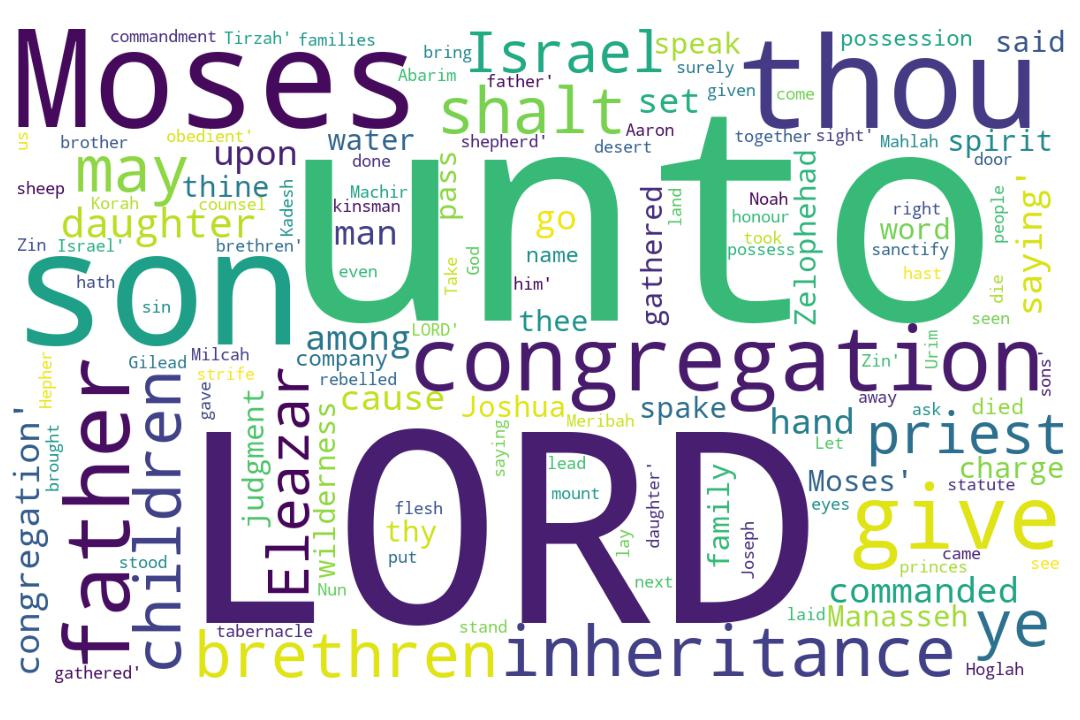
\includegraphics[width=\linewidth]{04OT-Numbers/Numbers27-WordCloud.jpg}
  \caption{Numbers 27 Word Cloud}
  \label{fig:Numbers 27 word Cloud}
\end{figure}

\marginpar{\scriptsize \centering \fcolorbox{blue}{lime}{\textbf{DAUGHTERS OF ZELOPHEHAD}}\\ (Numbers 27)
\begin{compactenum}[I.][8]
    \item \textbf{Single and Dispossessed} \index[scripture]{Numbers!Num 27:01--04} (Numbers 27:2--4)
    \item \textbf{Standing  before the Priests} \index[scripture]{Numbers!Num 27:02} (Numbers 27:2)
    \item A \textbf{Significant Problems} \index[scripture]{Numbers!Num 27:04} (Numbers 27:4)
    \item A \textbf{Sought Possession} \index[scripture]{Numbers!Num 27:04} (Numbers 27:4)
    \item The \textbf{Stated Plan} \index[scripture]{Numbers!Num 27:08--10} (Numbers 27:8--10)
\end{compactenum}}

%%%%%%%%%%%%%%%%%%%%%%%%%%%%%%%%%%
%%%%%%%%%%%%%%%%%%%%%%%%%%%%%%%%%%
\footnote{\textcolor[rgb]{0.00,0.25,0.00}{\hyperlink{TOC}{Return to end of Table of Contents.}}}\footnote{\href{https://audiobible.com/bible/numbers_27.html}{\textcolor[cmyk]{0.99998,1,0,0}{Numbers 27 Audio}}}\textcolor[cmyk]{0.99998,1,0,0}{Then came the daughters of Zelophehad, the son of Hepher, the son of Gilead, the son of Machir, the son of Manasseh, of the families of Manasseh the son of Joseph: and these \emph{are} the names of his daughters; Mahlah, Noah, and Hoglah, and Milcah, and Tirzah.}
[2] \textcolor[cmyk]{0.99998,1,0,0}{And they stood \fcolorbox{bone}{bone}{before} Moses, and \fcolorbox{bone}{bone}{before} Eleazar the priest, and \fcolorbox{bone}{bone}{before} the princes and all the congregation, \emph{by} the door of the tabernacle of the congregation, saying,}
[3] \textcolor[cmyk]{0.99998,1,0,0}{Our father died \fcolorbox{bone}{bone}{in} the wilderness, and he was not \fcolorbox{bone}{bone}{in} the company of them that gathered themselves together against the LORD \fcolorbox{bone}{bone}{in} the company of Korah; but died \fcolorbox{bone}{bone}{in} his own sin, and had no sons.}
[4] \textcolor[cmyk]{0.99998,1,0,0}{Why should the name of our father be done away from among his family, because he hath no son? Give unto us \emph{therefore} a possession among the brethren of our father.}
[5] \textcolor[cmyk]{0.99998,1,0,0}{And Moses brought their cause \fcolorbox{bone}{bone}{before} the LORD.}\\
\\
\P \textcolor[cmyk]{0.99998,1,0,0}{And the LORD spake unto Moses, saying,}
[7] \textcolor[cmyk]{0.99998,1,0,0}{The daughters of Zelophehad speak right: thou shalt surely give them a possession of an inheritance among their father's brethren; and thou shalt cause the inheritance of their father to pass unto them.}
[8] \textcolor[cmyk]{0.99998,1,0,0}{And thou shalt speak unto the children of Israel, saying, If a man die, and have no son, then ye shall cause his inheritance to pass unto his daughter.}
[9] \textcolor[cmyk]{0.99998,1,0,0}{And if he have no daughter, then ye shall give his inheritance unto his brethren.}
[10] \textcolor[cmyk]{0.99998,1,0,0}{And if he have no brethren, then ye shall give his inheritance unto his father's brethren.}
[11] \textcolor[cmyk]{0.99998,1,0,0}{And if his father have no brethren, then ye shall give his inheritance unto his kinsman that is next to him of his family, and he shall possess it: and it shall be unto the children of Israel a statute of judgment, as the LORD commanded Moses.}\\
\\
\P \textcolor[cmyk]{0.99998,1,0,0}{And the LORD said unto Moses, Get thee up into this mount Abarim, and see the land which I have given unto the children of Israel.}
[13] \textcolor[cmyk]{0.99998,1,0,0}{And when thou hast seen it, thou also shalt be gathered unto thy people, as Aaron thy brother was gathered.}
[14] \textcolor[cmyk]{0.99998,1,0,0}{For ye rebelled against my commandment \fcolorbox{bone}{bone}{in} the desert of Zin, \fcolorbox{bone}{bone}{in} the strife of the congregation, to sanctify me at the water \fcolorbox{bone}{bone}{before} their eyes: that \emph{is} the water of Meribah \fcolorbox{bone}{bone}{in} Kadesh \fcolorbox{bone}{bone}{in} the wilderness of Zin.}\\
\\
\P \textcolor[cmyk]{0.99998,1,0,0}{And Moses spake unto the LORD, saying,}
[16] \textcolor[cmyk]{0.99998,1,0,0}{Let the LORD, the God of the spirits of all flesh, set a man over the congregation,}
[17] \textcolor[cmyk]{0.99998,1,0,0}{Which may go out \fcolorbox{bone}{bone}{before} them, and which may go \fcolorbox{bone}{bone}{in} \fcolorbox{bone}{bone}{before} them, and which may lead them out, and which may bring them \fcolorbox{bone}{bone}{in}; that the congregation of the LORD be not as sheep which have no shepherd.}\\
\\
\P \textcolor[cmyk]{0.99998,1,0,0}{And the LORD said unto Moses, Take thee Joshua the son of Nun, a man \fcolorbox{bone}{bone}{in} whom \emph{is} the spirit, and lay thine hand upon him;}
[19] \textcolor[cmyk]{0.99998,1,0,0}{And set him \fcolorbox{bone}{bone}{before} Eleazar the priest, and \fcolorbox{bone}{bone}{before} all the congregation; and give him a charge \fcolorbox{bone}{bone}{in} their sight.}
[20] \textcolor[cmyk]{0.99998,1,0,0}{And thou shalt put \emph{some} of thine honour upon him, that all the congregation of the children of Israel may be obedient.}
[21] \textcolor[cmyk]{0.99998,1,0,0}{And he shall stand \fcolorbox{bone}{bone}{before} Eleazar the priest, who shall ask \emph{counsel} for him after the judgment of Urim \fcolorbox{bone}{bone}{before} the LORD: at his word shall they go out, and at his word they shall come \fcolorbox{bone}{bone}{in}, \emph{both} he, and all the children of Israel with him, even all the congregation.}
[22] \textcolor[cmyk]{0.99998,1,0,0}{And Moses did as the LORD commanded him: and he took Joshua, and set him \fcolorbox{bone}{bone}{before} Eleazar the priest, and \fcolorbox{bone}{bone}{before} all the congregation:}
[23] \textcolor[cmyk]{0.99998,1,0,0}{And he laid his hand upon him, and gave him a charge, as the LORD commanded by the hand of Moses.}
\index[NWIV]{47!Numbers!Num 27:1}\index[AWIP]{Then!Numbers!Num 27:1}\index[AWIP]{came!Numbers!Num 27:1}\index[AWIP]{the!Numbers!Num 27:1}\index[AWIP]{the!Numbers!Num 27:1 (2)}\index[AWIP]{the!Numbers!Num 27:1 (3)}\index[AWIP]{the!Numbers!Num 27:1 (4)}\index[AWIP]{the!Numbers!Num 27:1 (5)}\index[AWIP]{the!Numbers!Num 27:1 (6)}\index[AWIP]{the!Numbers!Num 27:1 (7)}\index[AWIP]{the!Numbers!Num 27:1 (8)}\index[AWIP]{daughters!Numbers!Num 27:1}\index[AWIP]{daughters!Numbers!Num 27:1 (2)}\index[AWIP]{of!Numbers!Num 27:1}\index[AWIP]{of!Numbers!Num 27:1 (2)}\index[AWIP]{of!Numbers!Num 27:1 (3)}\index[AWIP]{of!Numbers!Num 27:1 (4)}\index[AWIP]{of!Numbers!Num 27:1 (5)}\index[AWIP]{of!Numbers!Num 27:1 (6)}\index[AWIP]{of!Numbers!Num 27:1 (7)}\index[AWIP]{of!Numbers!Num 27:1 (8)}\index[AWIP]{of!Numbers!Num 27:1 (9)}\index[AWIP]{Zelophehad!Numbers!Num 27:1}\index[AWIP]{son!Numbers!Num 27:1}\index[AWIP]{son!Numbers!Num 27:1 (2)}\index[AWIP]{son!Numbers!Num 27:1 (3)}\index[AWIP]{son!Numbers!Num 27:1 (4)}\index[AWIP]{son!Numbers!Num 27:1 (5)}\index[AWIP]{Hepher!Numbers!Num 27:1}\index[AWIP]{Gilead!Numbers!Num 27:1}\index[AWIP]{Machir!Numbers!Num 27:1}\index[AWIP]{Manasseh!Numbers!Num 27:1}\index[AWIP]{Manasseh!Numbers!Num 27:1 (2)}\index[AWIP]{families!Numbers!Num 27:1}\index[AWIP]{Joseph!Numbers!Num 27:1}\index[AWIP]{and!Numbers!Num 27:1}\index[AWIP]{and!Numbers!Num 27:1 (2)}\index[AWIP]{and!Numbers!Num 27:1 (3)}\index[AWIP]{and!Numbers!Num 27:1 (4)}\index[AWIP]{these!Numbers!Num 27:1}\index[AWIP]{\emph{are}!Numbers!Num 27:1}\index[AWIP]{names!Numbers!Num 27:1}\index[AWIP]{his!Numbers!Num 27:1}\index[AWIP]{Mahlah!Numbers!Num 27:1}\index[AWIP]{Noah!Numbers!Num 27:1}\index[AWIP]{Hoglah!Numbers!Num 27:1}\index[AWIP]{Milcah!Numbers!Num 27:1}\index[AWIP]{Tirzah!Numbers!Num 27:1}\index[AWIP]{\emph{are}!Numbers!Num 27:1}

\index[NWIV]{28!Numbers!Num 27:2}\index[AWIP]{And!Numbers!Num 27:2}\index[AWIP]{they!Numbers!Num 27:2}\index[AWIP]{stood!Numbers!Num 27:2}\index[AWIP]{before!Numbers!Num 27:2}\index[AWIP]{before!Numbers!Num 27:2 (2)}\index[AWIP]{before!Numbers!Num 27:2 (3)}\index[AWIP]{Moses!Numbers!Num 27:2}\index[AWIP]{and!Numbers!Num 27:2}\index[AWIP]{and!Numbers!Num 27:2 (2)}\index[AWIP]{and!Numbers!Num 27:2 (3)}\index[AWIP]{Eleazar!Numbers!Num 27:2}\index[AWIP]{the!Numbers!Num 27:2}\index[AWIP]{the!Numbers!Num 27:2 (2)}\index[AWIP]{the!Numbers!Num 27:2 (3)}\index[AWIP]{the!Numbers!Num 27:2 (4)}\index[AWIP]{the!Numbers!Num 27:2 (5)}\index[AWIP]{the!Numbers!Num 27:2 (6)}\index[AWIP]{priest!Numbers!Num 27:2}\index[AWIP]{princes!Numbers!Num 27:2}\index[AWIP]{all!Numbers!Num 27:2}\index[AWIP]{congregation!Numbers!Num 27:2}\index[AWIP]{congregation!Numbers!Num 27:2 (2)}\index[AWIP]{\emph{by}!Numbers!Num 27:2}\index[AWIP]{door!Numbers!Num 27:2}\index[AWIP]{of!Numbers!Num 27:2}\index[AWIP]{of!Numbers!Num 27:2 (2)}\index[AWIP]{tabernacle!Numbers!Num 27:2}\index[AWIP]{saying!Numbers!Num 27:2}\index[AWIP]{\emph{by}!Numbers!Num 27:2}

\index[NWIV]{37!Numbers!Num 27:3}\index[AWIP]{Our!Numbers!Num 27:3}\index[AWIP]{father!Numbers!Num 27:3}\index[AWIP]{died!Numbers!Num 27:3}\index[AWIP]{died!Numbers!Num 27:3 (2)}\index[AWIP]{in!Numbers!Num 27:3}\index[AWIP]{in!Numbers!Num 27:3 (2)}\index[AWIP]{in!Numbers!Num 27:3 (3)}\index[AWIP]{in!Numbers!Num 27:3 (4)}\index[AWIP]{the!Numbers!Num 27:3}\index[AWIP]{the!Numbers!Num 27:3 (2)}\index[AWIP]{the!Numbers!Num 27:3 (3)}\index[AWIP]{the!Numbers!Num 27:3 (4)}\index[AWIP]{wilderness!Numbers!Num 27:3}\index[AWIP]{and!Numbers!Num 27:3}\index[AWIP]{and!Numbers!Num 27:3 (2)}\index[AWIP]{he!Numbers!Num 27:3}\index[AWIP]{was!Numbers!Num 27:3}\index[AWIP]{not!Numbers!Num 27:3}\index[AWIP]{company!Numbers!Num 27:3}\index[AWIP]{company!Numbers!Num 27:3 (2)}\index[AWIP]{of!Numbers!Num 27:3}\index[AWIP]{of!Numbers!Num 27:3 (2)}\index[AWIP]{them!Numbers!Num 27:3}\index[AWIP]{that!Numbers!Num 27:3}\index[AWIP]{gathered!Numbers!Num 27:3}\index[AWIP]{themselves!Numbers!Num 27:3}\index[AWIP]{together!Numbers!Num 27:3}\index[AWIP]{against!Numbers!Num 27:3}\index[AWIP]{LORD!Numbers!Num 27:3}\index[AWIP]{Korah!Numbers!Num 27:3}\index[AWIP]{but!Numbers!Num 27:3}\index[AWIP]{his!Numbers!Num 27:3}\index[AWIP]{own!Numbers!Num 27:3}\index[AWIP]{sin!Numbers!Num 27:3}\index[AWIP]{had!Numbers!Num 27:3}\index[AWIP]{no!Numbers!Num 27:3}\index[AWIP]{sons!Numbers!Num 27:3}

\index[NWIV]{31!Numbers!Num 27:4}\index[AWIP]{Why!Numbers!Num 27:4}\index[AWIP]{should!Numbers!Num 27:4}\index[AWIP]{the!Numbers!Num 27:4}\index[AWIP]{the!Numbers!Num 27:4 (2)}\index[AWIP]{name!Numbers!Num 27:4}\index[AWIP]{of!Numbers!Num 27:4}\index[AWIP]{of!Numbers!Num 27:4 (2)}\index[AWIP]{our!Numbers!Num 27:4}\index[AWIP]{our!Numbers!Num 27:4 (2)}\index[AWIP]{father!Numbers!Num 27:4}\index[AWIP]{father!Numbers!Num 27:4 (2)}\index[AWIP]{be!Numbers!Num 27:4}\index[AWIP]{done!Numbers!Num 27:4}\index[AWIP]{away!Numbers!Num 27:4}\index[AWIP]{from!Numbers!Num 27:4}\index[AWIP]{among!Numbers!Num 27:4}\index[AWIP]{among!Numbers!Num 27:4 (2)}\index[AWIP]{his!Numbers!Num 27:4}\index[AWIP]{family!Numbers!Num 27:4}\index[AWIP]{because!Numbers!Num 27:4}\index[AWIP]{he!Numbers!Num 27:4}\index[AWIP]{hath!Numbers!Num 27:4}\index[AWIP]{no!Numbers!Num 27:4}\index[AWIP]{son?!Numbers!Num 27:4}\index[AWIP]{Give!Numbers!Num 27:4}\index[AWIP]{unto!Numbers!Num 27:4}\index[AWIP]{us!Numbers!Num 27:4}\index[AWIP]{\emph{therefore}!Numbers!Num 27:4}\index[AWIP]{a!Numbers!Num 27:4}\index[AWIP]{possession!Numbers!Num 27:4}\index[AWIP]{brethren!Numbers!Num 27:4}\index[AWIP]{\emph{therefore}!Numbers!Num 27:4}

\index[NWIV]{8!Numbers!Num 27:5}\index[AWIP]{And!Numbers!Num 27:5}\index[AWIP]{Moses!Numbers!Num 27:5}\index[AWIP]{brought!Numbers!Num 27:5}\index[AWIP]{their!Numbers!Num 27:5}\index[AWIP]{cause!Numbers!Num 27:5}\index[AWIP]{before!Numbers!Num 27:5}\index[AWIP]{the!Numbers!Num 27:5}\index[AWIP]{LORD!Numbers!Num 27:5}

\index[NWIV]{7!Numbers!Num 27:6}\index[AWIP]{And!Numbers!Num 27:6}\index[AWIP]{the!Numbers!Num 27:6}\index[AWIP]{LORD!Numbers!Num 27:6}\index[AWIP]{spake!Numbers!Num 27:6}\index[AWIP]{unto!Numbers!Num 27:6}\index[AWIP]{Moses!Numbers!Num 27:6}\index[AWIP]{saying!Numbers!Num 27:6}

\index[NWIV]{33!Numbers!Num 27:7}\index[AWIP]{The!Numbers!Num 27:7}\index[AWIP]{daughters!Numbers!Num 27:7}\index[AWIP]{of!Numbers!Num 27:7}\index[AWIP]{of!Numbers!Num 27:7 (2)}\index[AWIP]{of!Numbers!Num 27:7 (3)}\index[AWIP]{Zelophehad!Numbers!Num 27:7}\index[AWIP]{speak!Numbers!Num 27:7}\index[AWIP]{right!Numbers!Num 27:7}\index[AWIP]{thou!Numbers!Num 27:7}\index[AWIP]{thou!Numbers!Num 27:7 (2)}\index[AWIP]{shalt!Numbers!Num 27:7}\index[AWIP]{shalt!Numbers!Num 27:7 (2)}\index[AWIP]{surely!Numbers!Num 27:7}\index[AWIP]{give!Numbers!Num 27:7}\index[AWIP]{them!Numbers!Num 27:7}\index[AWIP]{them!Numbers!Num 27:7 (2)}\index[AWIP]{a!Numbers!Num 27:7}\index[AWIP]{possession!Numbers!Num 27:7}\index[AWIP]{an!Numbers!Num 27:7}\index[AWIP]{inheritance!Numbers!Num 27:7}\index[AWIP]{inheritance!Numbers!Num 27:7 (2)}\index[AWIP]{among!Numbers!Num 27:7}\index[AWIP]{their!Numbers!Num 27:7}\index[AWIP]{their!Numbers!Num 27:7 (2)}\index[AWIP]{father's!Numbers!Num 27:7}\index[AWIP]{brethren!Numbers!Num 27:7}\index[AWIP]{and!Numbers!Num 27:7}\index[AWIP]{cause!Numbers!Num 27:7}\index[AWIP]{the!Numbers!Num 27:7}\index[AWIP]{father!Numbers!Num 27:7}\index[AWIP]{to!Numbers!Num 27:7}\index[AWIP]{pass!Numbers!Num 27:7}\index[AWIP]{unto!Numbers!Num 27:7}

\index[NWIV]{29!Numbers!Num 27:8}\index[AWIP]{And!Numbers!Num 27:8}\index[AWIP]{thou!Numbers!Num 27:8}\index[AWIP]{shalt!Numbers!Num 27:8}\index[AWIP]{speak!Numbers!Num 27:8}\index[AWIP]{unto!Numbers!Num 27:8}\index[AWIP]{unto!Numbers!Num 27:8 (2)}\index[AWIP]{the!Numbers!Num 27:8}\index[AWIP]{children!Numbers!Num 27:8}\index[AWIP]{of!Numbers!Num 27:8}\index[AWIP]{Israel!Numbers!Num 27:8}\index[AWIP]{saying!Numbers!Num 27:8}\index[AWIP]{If!Numbers!Num 27:8}\index[AWIP]{a!Numbers!Num 27:8}\index[AWIP]{man!Numbers!Num 27:8}\index[AWIP]{die!Numbers!Num 27:8}\index[AWIP]{and!Numbers!Num 27:8}\index[AWIP]{have!Numbers!Num 27:8}\index[AWIP]{no!Numbers!Num 27:8}\index[AWIP]{son!Numbers!Num 27:8}\index[AWIP]{then!Numbers!Num 27:8}\index[AWIP]{ye!Numbers!Num 27:8}\index[AWIP]{shall!Numbers!Num 27:8}\index[AWIP]{cause!Numbers!Num 27:8}\index[AWIP]{his!Numbers!Num 27:8}\index[AWIP]{his!Numbers!Num 27:8 (2)}\index[AWIP]{inheritance!Numbers!Num 27:8}\index[AWIP]{to!Numbers!Num 27:8}\index[AWIP]{pass!Numbers!Num 27:8}\index[AWIP]{daughter!Numbers!Num 27:8}

\index[NWIV]{15!Numbers!Num 27:9}\index[AWIP]{And!Numbers!Num 27:9}\index[AWIP]{if!Numbers!Num 27:9}\index[AWIP]{he!Numbers!Num 27:9}\index[AWIP]{have!Numbers!Num 27:9}\index[AWIP]{no!Numbers!Num 27:9}\index[AWIP]{daughter!Numbers!Num 27:9}\index[AWIP]{then!Numbers!Num 27:9}\index[AWIP]{ye!Numbers!Num 27:9}\index[AWIP]{shall!Numbers!Num 27:9}\index[AWIP]{give!Numbers!Num 27:9}\index[AWIP]{his!Numbers!Num 27:9}\index[AWIP]{his!Numbers!Num 27:9 (2)}\index[AWIP]{inheritance!Numbers!Num 27:9}\index[AWIP]{unto!Numbers!Num 27:9}\index[AWIP]{brethren!Numbers!Num 27:9}

\index[NWIV]{16!Numbers!Num 27:10}\index[AWIP]{And!Numbers!Num 27:10}\index[AWIP]{if!Numbers!Num 27:10}\index[AWIP]{he!Numbers!Num 27:10}\index[AWIP]{have!Numbers!Num 27:10}\index[AWIP]{no!Numbers!Num 27:10}\index[AWIP]{brethren!Numbers!Num 27:10}\index[AWIP]{brethren!Numbers!Num 27:10 (2)}\index[AWIP]{then!Numbers!Num 27:10}\index[AWIP]{ye!Numbers!Num 27:10}\index[AWIP]{shall!Numbers!Num 27:10}\index[AWIP]{give!Numbers!Num 27:10}\index[AWIP]{his!Numbers!Num 27:10}\index[AWIP]{his!Numbers!Num 27:10 (2)}\index[AWIP]{inheritance!Numbers!Num 27:10}\index[AWIP]{unto!Numbers!Num 27:10}\index[AWIP]{father's!Numbers!Num 27:10}

\index[NWIV]{47!Numbers!Num 27:11}\index[AWIP]{And!Numbers!Num 27:11}\index[AWIP]{if!Numbers!Num 27:11}\index[AWIP]{his!Numbers!Num 27:11}\index[AWIP]{his!Numbers!Num 27:11 (2)}\index[AWIP]{his!Numbers!Num 27:11 (3)}\index[AWIP]{his!Numbers!Num 27:11 (4)}\index[AWIP]{father!Numbers!Num 27:11}\index[AWIP]{have!Numbers!Num 27:11}\index[AWIP]{no!Numbers!Num 27:11}\index[AWIP]{brethren!Numbers!Num 27:11}\index[AWIP]{then!Numbers!Num 27:11}\index[AWIP]{ye!Numbers!Num 27:11}\index[AWIP]{shall!Numbers!Num 27:11}\index[AWIP]{shall!Numbers!Num 27:11 (2)}\index[AWIP]{shall!Numbers!Num 27:11 (3)}\index[AWIP]{give!Numbers!Num 27:11}\index[AWIP]{inheritance!Numbers!Num 27:11}\index[AWIP]{unto!Numbers!Num 27:11}\index[AWIP]{unto!Numbers!Num 27:11 (2)}\index[AWIP]{kinsman!Numbers!Num 27:11}\index[AWIP]{that!Numbers!Num 27:11}\index[AWIP]{is!Numbers!Num 27:11}\index[AWIP]{next!Numbers!Num 27:11}\index[AWIP]{to!Numbers!Num 27:11}\index[AWIP]{him!Numbers!Num 27:11}\index[AWIP]{of!Numbers!Num 27:11}\index[AWIP]{of!Numbers!Num 27:11 (2)}\index[AWIP]{of!Numbers!Num 27:11 (3)}\index[AWIP]{family!Numbers!Num 27:11}\index[AWIP]{and!Numbers!Num 27:11}\index[AWIP]{and!Numbers!Num 27:11 (2)}\index[AWIP]{he!Numbers!Num 27:11}\index[AWIP]{possess!Numbers!Num 27:11}\index[AWIP]{it!Numbers!Num 27:11}\index[AWIP]{it!Numbers!Num 27:11 (2)}\index[AWIP]{be!Numbers!Num 27:11}\index[AWIP]{the!Numbers!Num 27:11}\index[AWIP]{the!Numbers!Num 27:11 (2)}\index[AWIP]{children!Numbers!Num 27:11}\index[AWIP]{Israel!Numbers!Num 27:11}\index[AWIP]{a!Numbers!Num 27:11}\index[AWIP]{statute!Numbers!Num 27:11}\index[AWIP]{judgment!Numbers!Num 27:11}\index[AWIP]{as!Numbers!Num 27:11}\index[AWIP]{LORD!Numbers!Num 27:11}\index[AWIP]{commanded!Numbers!Num 27:11}\index[AWIP]{Moses!Numbers!Num 27:11}

\index[NWIV]{26!Numbers!Num 27:12}\index[AWIP]{And!Numbers!Num 27:12}\index[AWIP]{the!Numbers!Num 27:12}\index[AWIP]{the!Numbers!Num 27:12 (2)}\index[AWIP]{the!Numbers!Num 27:12 (3)}\index[AWIP]{LORD!Numbers!Num 27:12}\index[AWIP]{said!Numbers!Num 27:12}\index[AWIP]{unto!Numbers!Num 27:12}\index[AWIP]{unto!Numbers!Num 27:12 (2)}\index[AWIP]{Moses!Numbers!Num 27:12}\index[AWIP]{Get!Numbers!Num 27:12}\index[AWIP]{thee!Numbers!Num 27:12}\index[AWIP]{up!Numbers!Num 27:12}\index[AWIP]{into!Numbers!Num 27:12}\index[AWIP]{this!Numbers!Num 27:12}\index[AWIP]{mount!Numbers!Num 27:12}\index[AWIP]{Abarim!Numbers!Num 27:12}\index[AWIP]{and!Numbers!Num 27:12}\index[AWIP]{see!Numbers!Num 27:12}\index[AWIP]{land!Numbers!Num 27:12}\index[AWIP]{which!Numbers!Num 27:12}\index[AWIP]{I!Numbers!Num 27:12}\index[AWIP]{have!Numbers!Num 27:12}\index[AWIP]{given!Numbers!Num 27:12}\index[AWIP]{children!Numbers!Num 27:12}\index[AWIP]{of!Numbers!Num 27:12}\index[AWIP]{Israel!Numbers!Num 27:12}

\index[NWIV]{20!Numbers!Num 27:13}\index[AWIP]{And!Numbers!Num 27:13}\index[AWIP]{when!Numbers!Num 27:13}\index[AWIP]{thou!Numbers!Num 27:13}\index[AWIP]{thou!Numbers!Num 27:13 (2)}\index[AWIP]{hast!Numbers!Num 27:13}\index[AWIP]{seen!Numbers!Num 27:13}\index[AWIP]{it!Numbers!Num 27:13}\index[AWIP]{also!Numbers!Num 27:13}\index[AWIP]{shalt!Numbers!Num 27:13}\index[AWIP]{be!Numbers!Num 27:13}\index[AWIP]{gathered!Numbers!Num 27:13}\index[AWIP]{gathered!Numbers!Num 27:13 (2)}\index[AWIP]{unto!Numbers!Num 27:13}\index[AWIP]{thy!Numbers!Num 27:13}\index[AWIP]{thy!Numbers!Num 27:13 (2)}\index[AWIP]{people!Numbers!Num 27:13}\index[AWIP]{as!Numbers!Num 27:13}\index[AWIP]{Aaron!Numbers!Num 27:13}\index[AWIP]{brother!Numbers!Num 27:13}\index[AWIP]{was!Numbers!Num 27:13}

\index[NWIV]{39!Numbers!Num 27:14}\index[AWIP]{For!Numbers!Num 27:14}\index[AWIP]{ye!Numbers!Num 27:14}\index[AWIP]{rebelled!Numbers!Num 27:14}\index[AWIP]{against!Numbers!Num 27:14}\index[AWIP]{my!Numbers!Num 27:14}\index[AWIP]{commandment!Numbers!Num 27:14}\index[AWIP]{in!Numbers!Num 27:14}\index[AWIP]{in!Numbers!Num 27:14 (2)}\index[AWIP]{in!Numbers!Num 27:14 (3)}\index[AWIP]{in!Numbers!Num 27:14 (4)}\index[AWIP]{the!Numbers!Num 27:14}\index[AWIP]{the!Numbers!Num 27:14 (2)}\index[AWIP]{the!Numbers!Num 27:14 (3)}\index[AWIP]{the!Numbers!Num 27:14 (4)}\index[AWIP]{the!Numbers!Num 27:14 (5)}\index[AWIP]{the!Numbers!Num 27:14 (6)}\index[AWIP]{desert!Numbers!Num 27:14}\index[AWIP]{of!Numbers!Num 27:14}\index[AWIP]{of!Numbers!Num 27:14 (2)}\index[AWIP]{of!Numbers!Num 27:14 (3)}\index[AWIP]{of!Numbers!Num 27:14 (4)}\index[AWIP]{Zin!Numbers!Num 27:14}\index[AWIP]{Zin!Numbers!Num 27:14 (2)}\index[AWIP]{strife!Numbers!Num 27:14}\index[AWIP]{congregation!Numbers!Num 27:14}\index[AWIP]{to!Numbers!Num 27:14}\index[AWIP]{sanctify!Numbers!Num 27:14}\index[AWIP]{me!Numbers!Num 27:14}\index[AWIP]{at!Numbers!Num 27:14}\index[AWIP]{water!Numbers!Num 27:14}\index[AWIP]{water!Numbers!Num 27:14 (2)}\index[AWIP]{before!Numbers!Num 27:14}\index[AWIP]{their!Numbers!Num 27:14}\index[AWIP]{eyes!Numbers!Num 27:14}\index[AWIP]{that!Numbers!Num 27:14}\index[AWIP]{\emph{is}!Numbers!Num 27:14}\index[AWIP]{Meribah!Numbers!Num 27:14}\index[AWIP]{Kadesh!Numbers!Num 27:14}\index[AWIP]{wilderness!Numbers!Num 27:14}\index[AWIP]{\emph{is}!Numbers!Num 27:14}

\index[NWIV]{7!Numbers!Num 27:15}\index[AWIP]{And!Numbers!Num 27:15}\index[AWIP]{Moses!Numbers!Num 27:15}\index[AWIP]{spake!Numbers!Num 27:15}\index[AWIP]{unto!Numbers!Num 27:15}\index[AWIP]{the!Numbers!Num 27:15}\index[AWIP]{LORD!Numbers!Num 27:15}\index[AWIP]{saying!Numbers!Num 27:15}

\index[NWIV]{17!Numbers!Num 27:16}\index[AWIP]{Let!Numbers!Num 27:16}\index[AWIP]{the!Numbers!Num 27:16}\index[AWIP]{the!Numbers!Num 27:16 (2)}\index[AWIP]{the!Numbers!Num 27:16 (3)}\index[AWIP]{the!Numbers!Num 27:16 (4)}\index[AWIP]{LORD!Numbers!Num 27:16}\index[AWIP]{God!Numbers!Num 27:16}\index[AWIP]{of!Numbers!Num 27:16}\index[AWIP]{of!Numbers!Num 27:16 (2)}\index[AWIP]{spirits!Numbers!Num 27:16}\index[AWIP]{all!Numbers!Num 27:16}\index[AWIP]{flesh!Numbers!Num 27:16}\index[AWIP]{set!Numbers!Num 27:16}\index[AWIP]{a!Numbers!Num 27:16}\index[AWIP]{man!Numbers!Num 27:16}\index[AWIP]{over!Numbers!Num 27:16}\index[AWIP]{congregation!Numbers!Num 27:16}

\index[NWIV]{39!Numbers!Num 27:17}\index[AWIP]{Which!Numbers!Num 27:17}\index[AWIP]{may!Numbers!Num 27:17}\index[AWIP]{may!Numbers!Num 27:17 (2)}\index[AWIP]{may!Numbers!Num 27:17 (3)}\index[AWIP]{may!Numbers!Num 27:17 (4)}\index[AWIP]{go!Numbers!Num 27:17}\index[AWIP]{go!Numbers!Num 27:17 (2)}\index[AWIP]{out!Numbers!Num 27:17}\index[AWIP]{out!Numbers!Num 27:17 (2)}\index[AWIP]{before!Numbers!Num 27:17}\index[AWIP]{before!Numbers!Num 27:17 (2)}\index[AWIP]{them!Numbers!Num 27:17}\index[AWIP]{them!Numbers!Num 27:17 (2)}\index[AWIP]{them!Numbers!Num 27:17 (3)}\index[AWIP]{them!Numbers!Num 27:17 (4)}\index[AWIP]{and!Numbers!Num 27:17}\index[AWIP]{and!Numbers!Num 27:17 (2)}\index[AWIP]{and!Numbers!Num 27:17 (3)}\index[AWIP]{which!Numbers!Num 27:17}\index[AWIP]{which!Numbers!Num 27:17 (2)}\index[AWIP]{which!Numbers!Num 27:17 (3)}\index[AWIP]{which!Numbers!Num 27:17 (4)}\index[AWIP]{in!Numbers!Num 27:17}\index[AWIP]{in!Numbers!Num 27:17 (2)}\index[AWIP]{lead!Numbers!Num 27:17}\index[AWIP]{bring!Numbers!Num 27:17}\index[AWIP]{that!Numbers!Num 27:17}\index[AWIP]{the!Numbers!Num 27:17}\index[AWIP]{the!Numbers!Num 27:17 (2)}\index[AWIP]{congregation!Numbers!Num 27:17}\index[AWIP]{of!Numbers!Num 27:17}\index[AWIP]{LORD!Numbers!Num 27:17}\index[AWIP]{be!Numbers!Num 27:17}\index[AWIP]{not!Numbers!Num 27:17}\index[AWIP]{as!Numbers!Num 27:17}\index[AWIP]{sheep!Numbers!Num 27:17}\index[AWIP]{have!Numbers!Num 27:17}\index[AWIP]{no!Numbers!Num 27:17}\index[AWIP]{shepherd!Numbers!Num 27:17}

\index[NWIV]{26!Numbers!Num 27:18}\index[AWIP]{And!Numbers!Num 27:18}\index[AWIP]{the!Numbers!Num 27:18}\index[AWIP]{the!Numbers!Num 27:18 (2)}\index[AWIP]{the!Numbers!Num 27:18 (3)}\index[AWIP]{LORD!Numbers!Num 27:18}\index[AWIP]{said!Numbers!Num 27:18}\index[AWIP]{unto!Numbers!Num 27:18}\index[AWIP]{Moses!Numbers!Num 27:18}\index[AWIP]{Take!Numbers!Num 27:18}\index[AWIP]{thee!Numbers!Num 27:18}\index[AWIP]{Joshua!Numbers!Num 27:18}\index[AWIP]{son!Numbers!Num 27:18}\index[AWIP]{of!Numbers!Num 27:18}\index[AWIP]{Nun!Numbers!Num 27:18}\index[AWIP]{a!Numbers!Num 27:18}\index[AWIP]{man!Numbers!Num 27:18}\index[AWIP]{in!Numbers!Num 27:18}\index[AWIP]{whom!Numbers!Num 27:18}\index[AWIP]{\emph{is}!Numbers!Num 27:18}\index[AWIP]{spirit!Numbers!Num 27:18}\index[AWIP]{and!Numbers!Num 27:18}\index[AWIP]{lay!Numbers!Num 27:18}\index[AWIP]{thine!Numbers!Num 27:18}\index[AWIP]{hand!Numbers!Num 27:18}\index[AWIP]{upon!Numbers!Num 27:18}\index[AWIP]{him!Numbers!Num 27:18}\index[AWIP]{\emph{is}!Numbers!Num 27:18}

\index[NWIV]{20!Numbers!Num 27:19}\index[AWIP]{And!Numbers!Num 27:19}\index[AWIP]{set!Numbers!Num 27:19}\index[AWIP]{him!Numbers!Num 27:19}\index[AWIP]{him!Numbers!Num 27:19 (2)}\index[AWIP]{before!Numbers!Num 27:19}\index[AWIP]{before!Numbers!Num 27:19 (2)}\index[AWIP]{Eleazar!Numbers!Num 27:19}\index[AWIP]{the!Numbers!Num 27:19}\index[AWIP]{the!Numbers!Num 27:19 (2)}\index[AWIP]{priest!Numbers!Num 27:19}\index[AWIP]{and!Numbers!Num 27:19}\index[AWIP]{and!Numbers!Num 27:19 (2)}\index[AWIP]{all!Numbers!Num 27:19}\index[AWIP]{congregation!Numbers!Num 27:19}\index[AWIP]{give!Numbers!Num 27:19}\index[AWIP]{a!Numbers!Num 27:19}\index[AWIP]{charge!Numbers!Num 27:19}\index[AWIP]{in!Numbers!Num 27:19}\index[AWIP]{their!Numbers!Num 27:19}\index[AWIP]{sight!Numbers!Num 27:19}

\index[NWIV]{22!Numbers!Num 27:20}\index[AWIP]{And!Numbers!Num 27:20}\index[AWIP]{thou!Numbers!Num 27:20}\index[AWIP]{shalt!Numbers!Num 27:20}\index[AWIP]{put!Numbers!Num 27:20}\index[AWIP]{\emph{some}!Numbers!Num 27:20}\index[AWIP]{of!Numbers!Num 27:20}\index[AWIP]{of!Numbers!Num 27:20 (2)}\index[AWIP]{of!Numbers!Num 27:20 (3)}\index[AWIP]{thine!Numbers!Num 27:20}\index[AWIP]{honour!Numbers!Num 27:20}\index[AWIP]{upon!Numbers!Num 27:20}\index[AWIP]{him!Numbers!Num 27:20}\index[AWIP]{that!Numbers!Num 27:20}\index[AWIP]{all!Numbers!Num 27:20}\index[AWIP]{the!Numbers!Num 27:20}\index[AWIP]{the!Numbers!Num 27:20 (2)}\index[AWIP]{congregation!Numbers!Num 27:20}\index[AWIP]{children!Numbers!Num 27:20}\index[AWIP]{Israel!Numbers!Num 27:20}\index[AWIP]{may!Numbers!Num 27:20}\index[AWIP]{be!Numbers!Num 27:20}\index[AWIP]{obedient!Numbers!Num 27:20}\index[AWIP]{\emph{some}!Numbers!Num 27:20}

\index[NWIV]{51!Numbers!Num 27:21}\index[AWIP]{And!Numbers!Num 27:21}\index[AWIP]{he!Numbers!Num 27:21}\index[AWIP]{he!Numbers!Num 27:21 (2)}\index[AWIP]{shall!Numbers!Num 27:21}\index[AWIP]{shall!Numbers!Num 27:21 (2)}\index[AWIP]{shall!Numbers!Num 27:21 (3)}\index[AWIP]{shall!Numbers!Num 27:21 (4)}\index[AWIP]{stand!Numbers!Num 27:21}\index[AWIP]{before!Numbers!Num 27:21}\index[AWIP]{before!Numbers!Num 27:21 (2)}\index[AWIP]{Eleazar!Numbers!Num 27:21}\index[AWIP]{the!Numbers!Num 27:21}\index[AWIP]{the!Numbers!Num 27:21 (2)}\index[AWIP]{the!Numbers!Num 27:21 (3)}\index[AWIP]{the!Numbers!Num 27:21 (4)}\index[AWIP]{the!Numbers!Num 27:21 (5)}\index[AWIP]{priest!Numbers!Num 27:21}\index[AWIP]{who!Numbers!Num 27:21}\index[AWIP]{ask!Numbers!Num 27:21}\index[AWIP]{\emph{counsel}!Numbers!Num 27:21}\index[AWIP]{for!Numbers!Num 27:21}\index[AWIP]{him!Numbers!Num 27:21}\index[AWIP]{him!Numbers!Num 27:21 (2)}\index[AWIP]{after!Numbers!Num 27:21}\index[AWIP]{judgment!Numbers!Num 27:21}\index[AWIP]{of!Numbers!Num 27:21}\index[AWIP]{of!Numbers!Num 27:21 (2)}\index[AWIP]{Urim!Numbers!Num 27:21}\index[AWIP]{LORD!Numbers!Num 27:21}\index[AWIP]{at!Numbers!Num 27:21}\index[AWIP]{at!Numbers!Num 27:21 (2)}\index[AWIP]{his!Numbers!Num 27:21}\index[AWIP]{his!Numbers!Num 27:21 (2)}\index[AWIP]{word!Numbers!Num 27:21}\index[AWIP]{word!Numbers!Num 27:21 (2)}\index[AWIP]{they!Numbers!Num 27:21}\index[AWIP]{they!Numbers!Num 27:21 (2)}\index[AWIP]{go!Numbers!Num 27:21}\index[AWIP]{out!Numbers!Num 27:21}\index[AWIP]{and!Numbers!Num 27:21}\index[AWIP]{and!Numbers!Num 27:21 (2)}\index[AWIP]{come!Numbers!Num 27:21}\index[AWIP]{in!Numbers!Num 27:21}\index[AWIP]{\emph{both}!Numbers!Num 27:21}\index[AWIP]{all!Numbers!Num 27:21}\index[AWIP]{all!Numbers!Num 27:21 (2)}\index[AWIP]{children!Numbers!Num 27:21}\index[AWIP]{Israel!Numbers!Num 27:21}\index[AWIP]{with!Numbers!Num 27:21}\index[AWIP]{even!Numbers!Num 27:21}\index[AWIP]{congregation!Numbers!Num 27:21}\index[AWIP]{\emph{counsel}!Numbers!Num 27:21}\index[AWIP]{\emph{both}!Numbers!Num 27:21}

\index[NWIV]{24!Numbers!Num 27:22}\index[AWIP]{And!Numbers!Num 27:22}\index[AWIP]{Moses!Numbers!Num 27:22}\index[AWIP]{did!Numbers!Num 27:22}\index[AWIP]{as!Numbers!Num 27:22}\index[AWIP]{the!Numbers!Num 27:22}\index[AWIP]{the!Numbers!Num 27:22 (2)}\index[AWIP]{the!Numbers!Num 27:22 (3)}\index[AWIP]{LORD!Numbers!Num 27:22}\index[AWIP]{commanded!Numbers!Num 27:22}\index[AWIP]{him!Numbers!Num 27:22}\index[AWIP]{him!Numbers!Num 27:22 (2)}\index[AWIP]{and!Numbers!Num 27:22}\index[AWIP]{and!Numbers!Num 27:22 (2)}\index[AWIP]{and!Numbers!Num 27:22 (3)}\index[AWIP]{he!Numbers!Num 27:22}\index[AWIP]{took!Numbers!Num 27:22}\index[AWIP]{Joshua!Numbers!Num 27:22}\index[AWIP]{set!Numbers!Num 27:22}\index[AWIP]{before!Numbers!Num 27:22}\index[AWIP]{before!Numbers!Num 27:22 (2)}\index[AWIP]{Eleazar!Numbers!Num 27:22}\index[AWIP]{priest!Numbers!Num 27:22}\index[AWIP]{all!Numbers!Num 27:22}\index[AWIP]{congregation!Numbers!Num 27:22}

\index[NWIV]{21!Numbers!Num 27:23}\index[AWIP]{And!Numbers!Num 27:23}\index[AWIP]{he!Numbers!Num 27:23}\index[AWIP]{laid!Numbers!Num 27:23}\index[AWIP]{his!Numbers!Num 27:23}\index[AWIP]{hands!Numbers!Num 27:23}\index[AWIP]{upon!Numbers!Num 27:23}\index[AWIP]{him!Numbers!Num 27:23}\index[AWIP]{him!Numbers!Num 27:23 (2)}\index[AWIP]{and!Numbers!Num 27:23}\index[AWIP]{gave!Numbers!Num 27:23}\index[AWIP]{a!Numbers!Num 27:23}\index[AWIP]{charge!Numbers!Num 27:23}\index[AWIP]{as!Numbers!Num 27:23}\index[AWIP]{the!Numbers!Num 27:23}\index[AWIP]{the!Numbers!Num 27:23 (2)}\index[AWIP]{LORD!Numbers!Num 27:23}\index[AWIP]{commanded!Numbers!Num 27:23}\index[AWIP]{by!Numbers!Num 27:23}\index[AWIP]{hand!Numbers!Num 27:23}\index[AWIP]{of!Numbers!Num 27:23}\index[AWIP]{Moses!Numbers!Num 27:23}


\section{Numbers 27 Outlines}

\subsection{My Outlines}

\subsubsection{The Daughters of Zelophehad}
\index[speaker]{Keith Anthony!Numbers 27 (The Daughters of Zelophehad)}
\index[series]{Numbers (Keith Anthony)!Numbers 27 (The Daughters of Zelophehad)}
\index[date]{2017/02/18!Numbers 27 (The Daughters of Zelophehad) (Keith Anthony)}
\begin{compactenum}[I.][7]
    \item \textbf{Single and Dispossessed} \index[scripture]{Numbers!Num 27:01--04} (Numbers 27:2--4)
    \item \textbf{Standing before the Priests} \index[scripture]{Numbers!Num 27:02} (Numbers 27:2)
    \item A \textbf{Significant Problems} \index[scripture]{Numbers!Num 27:04} (Numbers 27:4)
    \item A \textbf{Sought Possession} \index[scripture]{Numbers!Num 27:04} (Numbers 27:4)
    \item The \textbf{Stated Plan} \index[scripture]{Numbers!Num 27:08--10} (Numbers 27:8--10)
\end{compactenum}

\subsection{Outlines from Others}



\section{Numbers 27 Comments}

\subsection{Numeric Nuggets}
\textbf{13: } Verse 16 has 13 unique words. The words ``before'' and ``in'' are used 13 times in the chapter.


\subsection{Numbers 27 Repeated Phrases}


%%%%%%%%%%
%%%%%%%%%%
\normalsize
 
\begin{center}
\begin{longtable}{|p{3.0in}|p{0.5in}|}
\caption[Numbers 27 Repeated Phrases]{Numbers 27 Repeated Phrases}\label{table:Repeated Phrases Numbers 27} \\
\hline \multicolumn{1}{|c|}{\textbf{Phrase}} & \multicolumn{1}{c|}{\textbf{Frequency}} \\ \hline 
\endfirsthead
 
\multicolumn{2}{c}
{{\bfseries \tablename\ \thetable{} -- continued from previous page}} \\  
\hline \multicolumn{1}{|c|}{\textbf{Phrase}} & \multicolumn{1}{c|}{\textbf{Frequency}} \\ \hline 
\endhead
 
\hline \multicolumn{2}{c}{{ }} \\ \hline
\endfoot 
the LORD & 12\\ \hline 
the congregation & 9\\ \hline 
of the & 7\\ \hline 
the son & 6\\ \hline 
the son of & 6\\ \hline 
son of & 6\\ \hline 
all the & 6\\ \hline 
in the & 6\\ \hline 
all the congregation & 5\\ \hline 
the children & 5\\ \hline 
the children of & 5\\ \hline 
the children of Israel & 5\\ \hline 
children of & 5\\ \hline 
children of Israel & 5\\ \hline 
of Israel & 5\\ \hline 
have no & 5\\ \hline 
and before & 4\\ \hline 
before Eleazar & 4\\ \hline 
before Eleazar the & 4\\ \hline 
before Eleazar the priest & 4\\ \hline 
Eleazar the & 4\\ \hline 
Eleazar the priest & 4\\ \hline 
the priest & 4\\ \hline 
thou shalt & 4\\ \hline 
unto the & 4\\ \hline 
then ye & 4\\ \hline 
then ye shall & 4\\ \hline 
ye shall & 4\\ \hline 
his inheritance & 4\\ \hline 
unto his & 4\\ \hline 
before Eleazar the priest and & 3\\ \hline 
before Eleazar the priest and before & 3\\ \hline 
Eleazar the priest and & 3\\ \hline 
Eleazar the priest and before & 3\\ \hline 
the priest and & 3\\ \hline 
the priest and before & 3\\ \hline 
priest and & 3\\ \hline 
priest and before & 3\\ \hline 
before the & 3\\ \hline 
and he & 3\\ \hline 
And Moses & 3\\ \hline 
And the & 3\\ \hline 
And the LORD & 3\\ \hline 
unto Moses & 3\\ \hline 
unto the children & 3\\ \hline 
unto the children of & 3\\ \hline 
unto the children of Israel & 3\\ \hline 
a man & 3\\ \hline 
And if & 3\\ \hline 
then ye shall give & 3\\ \hline 
then ye shall give his & 3\\ \hline 
then ye shall give his inheritance & 3\\ \hline 
then ye shall give his inheritance unto & 3\\ \hline 
then ye shall give his inheritance unto his & 3\\ \hline 
ye shall give & 3\\ \hline 
ye shall give his & 3\\ \hline 
ye shall give his inheritance & 3\\ \hline 
ye shall give his inheritance unto & 3\\ \hline 
ye shall give his inheritance unto his & 3\\ \hline 
shall give & 3\\ \hline 
shall give his & 3\\ \hline 
shall give his inheritance & 3\\ \hline 
shall give his inheritance unto & 3\\ \hline 
shall give his inheritance unto his & 3\\ \hline 
give his & 3\\ \hline 
give his inheritance & 3\\ \hline 
give his inheritance unto & 3\\ \hline 
give his inheritance unto his & 3\\ \hline 
his inheritance unto & 3\\ \hline 
his inheritance unto his & 3\\ \hline 
inheritance unto & 3\\ \hline 
inheritance unto his & 3\\ \hline 
as the & 3\\ \hline 
as the LORD & 3\\ \hline 
as the LORD commanded & 3\\ \hline 
the LORD commanded & 3\\ \hline 
LORD commanded & 3\\ \hline 
and which & 3\\ \hline 
and which may & 3\\ \hline 
which may & 3\\ \hline 
upon him & 3\\ \hline 
\end{longtable}
\end{center}



%%%%%%%%%%
%%%%%%%%%%



\section{Numbers 27 Word Statistics}


%%%%%%%%%%
%%%%%%%%%%
\normalsize
 
\begin{center}
\begin{longtable}{l|c|c|c|c}
\caption[Numbers 27 Statistics]{Numbers 27 Statistics}\label{table:Statistics for Numbers 27} \\
\hline \multicolumn{1}{|c|}{\textbf{Verse(s)}} & \multicolumn{1}{|c|}{\textbf{Count}} & \multicolumn{1}{|c|}{\textbf{Unique}} & \multicolumn{1}{|c|}{\textbf{Italics}} & \multicolumn{1}{|c|}{\textbf{Uniq Italic}}  \\ \hline 
\endfirsthead
 
\multicolumn{5}{c}
{{\bfseries \tablename\ \thetable{} -- continued from previous page}} \\  
\hline \multicolumn{1}{|c|}{\textbf{Verse(s)}} & \multicolumn{1}{|c|}{\textbf{Count}} & \multicolumn{1}{|c|}{\textbf{Unique}} & \multicolumn{1}{|c|}{\textbf{Italics}} & \multicolumn{1}{|c|}{\textbf{Uniq Italic}}  \\ \hline 
\endhead
 
\hline \multicolumn{5}{|r|}{{Continued if needed}} \\ \hline
\endfoot 
1 & 47 & 23 & 1 & 1\\ \hline
2 & 28 & 17 & 1 & 1\\ \hline
3 & 37 & 27 & 0 & 0\\ \hline
4 & 31 & 26 & 1 & 1\\ \hline
5 & 8 & 8 & 0 & 0\\ \hline
6 & 7 & 7 & 0 & 0\\ \hline
7 & 33 & 26 & 0 & 0\\ \hline
8 & 29 & 27 & 0 & 0\\ \hline
9 & 15 & 14 & 0 & 0\\ \hline
10 & 16 & 14 & 0 & 0\\ \hline
11 & 47 & 36 & 0 & 0\\ \hline
12 & 26 & 23 & 0 & 0\\ \hline
13 & 20 & 17 & 0 & 0\\ \hline
14 & 39 & 26 & 1 & 1\\ \hline
15 & 7 & 7 & 0 & 0\\ \hline
16 & 17 & 13 & 0 & 0\\ \hline
17 & 39 & 23 & 0 & 0\\ \hline
18 & 26 & 24 & 1 & 1\\ \hline
19 & 20 & 16 & 0 & 0\\ \hline
20 & 22 & 19 & 1 & 1\\ \hline
21 & 51 & 34 & 2 & 2\\ \hline
22 & 24 & 18 & 0 & 0\\ \hline
23 & 21 & 19 & 0 & 0\\ \hline
Total & 610 & 199 & 8 & 7
\end{longtable}
\end{center}



%%%%%%%%%%
%%%%%%%%%%


\subsection{Numbers 27 Words by Frequency}


%%%%%%%%%%
%%%%%%%%%%
\normalsize
 
\begin{center}
\begin{longtable}{l|r}
\caption[Numbers 27 Words by Frequency]{Numbers 27 Words by Frequency}\label{table:WordsbyFrequency for Numbers 27} \\
\hline \multicolumn{1}{|c|}{\textbf{Word}} & \multicolumn{1}{c|}{\textbf{Frequency}} \\ \hline 
\endfirsthead
 
\multicolumn{2}{c}
{{\bfseries \tablename\ \thetable{} -- continued from previous page}} \\  
\hline \multicolumn{1}{|c|}{\textbf{Word}} & \multicolumn{1}{c|}{\textbf{Frequency}} \\ \hline 
\endhead
 
\hline \multicolumn{2}{c}{{ }} \\ \hline
\endfoot 
the & 59\\ \hline 
of & 37\\ \hline 
and & 26\\ \hline 
his & 16\\ \hline 
And & 16\\ \hline 
unto & 14\\ \hline 
before & 13\\ \hline 
in & 13\\ \hline 
LORD & 12\\ \hline 
him & 11\\ \hline 
shall & 10\\ \hline 
Moses & 9\\ \hline 
congregation & 9\\ \hline 
he & 9\\ \hline 
son & 8\\ \hline 
a & 8\\ \hline 
all & 7\\ \hline 
them & 7\\ \hline 
no & 7\\ \hline 
brethren & 6\\ \hline 
thou & 6\\ \hline 
inheritance & 6\\ \hline 
have & 6\\ \hline 
father & 5\\ \hline 
that & 5\\ \hline 
be & 5\\ \hline 
their & 5\\ \hline 
shalt & 5\\ \hline 
give & 5\\ \hline 
children & 5\\ \hline 
Israel & 5\\ \hline 
ye & 5\\ \hline 
as & 5\\ \hline 
which & 5\\ \hline 
may & 5\\ \hline 
Eleazar & 4\\ \hline 
priest & 4\\ \hline 
saying & 4\\ \hline 
to & 4\\ \hline 
then & 4\\ \hline 
daughters & 3\\ \hline 
they & 3\\ \hline 
gathered & 3\\ \hline 
among & 3\\ \hline 
cause & 3\\ \hline 
man & 3\\ \hline 
if & 3\\ \hline 
it & 3\\ \hline 
commanded & 3\\ \hline 
at & 3\\ \hline 
set & 3\\ \hline 
go & 3\\ \hline 
out & 3\\ \hline 
upon & 3\\ \hline 
Zelophehad & 2\\ \hline 
Manasseh & 2\\ \hline 
died & 2\\ \hline 
wilderness & 2\\ \hline 
was & 2\\ \hline 
not & 2\\ \hline 
company & 2\\ \hline 
against & 2\\ \hline 
our & 2\\ \hline 
family & 2\\ \hline 
possession & 2\\ \hline 
spake & 2\\ \hline 
speak & 2\\ \hline 
father's & 2\\ \hline 
pass & 2\\ \hline 
daughter & 2\\ \hline 
judgment & 2\\ \hline 
said & 2\\ \hline 
thee & 2\\ \hline 
thy & 2\\ \hline 
Zin & 2\\ \hline 
water & 2\\ \hline 
\emph{is} & 2\\ \hline 
Joshua & 2\\ \hline 
thine & 2\\ \hline 
hand & 2\\ \hline 
charge & 2\\ \hline 
word & 2\\ \hline 
Then & 1\\ \hline 
came & 1\\ \hline 
Hepher & 1\\ \hline 
Gilead & 1\\ \hline 
Machir & 1\\ \hline 
families & 1\\ \hline 
Joseph & 1\\ \hline 
these & 1\\ \hline 
\emph{are} & 1\\ \hline 
names & 1\\ \hline 
Mahlah & 1\\ \hline 
Noah & 1\\ \hline 
Hoglah & 1\\ \hline 
Milcah & 1\\ \hline 
Tirzah & 1\\ \hline 
stood & 1\\ \hline 
princes & 1\\ \hline 
\emph{by} & 1\\ \hline 
door & 1\\ \hline 
tabernacle & 1\\ \hline 
Our & 1\\ \hline 
themselves & 1\\ \hline 
together & 1\\ \hline 
Korah & 1\\ \hline 
but & 1\\ \hline 
own & 1\\ \hline 
sin & 1\\ \hline 
had & 1\\ \hline 
sons & 1\\ \hline 
Why & 1\\ \hline 
should & 1\\ \hline 
name & 1\\ \hline 
done & 1\\ \hline 
away & 1\\ \hline 
from & 1\\ \hline 
because & 1\\ \hline 
hath & 1\\ \hline 
Give & 1\\ \hline 
us & 1\\ \hline 
\emph{therefore} & 1\\ \hline 
brought & 1\\ \hline 
The & 1\\ \hline 
right & 1\\ \hline 
surely & 1\\ \hline 
an & 1\\ \hline 
If & 1\\ \hline 
die & 1\\ \hline 
kinsman & 1\\ \hline 
is & 1\\ \hline 
next & 1\\ \hline 
possess & 1\\ \hline 
statute & 1\\ \hline 
Get & 1\\ \hline 
up & 1\\ \hline 
into & 1\\ \hline 
this & 1\\ \hline 
mount & 1\\ \hline 
Abarim & 1\\ \hline 
see & 1\\ \hline 
land & 1\\ \hline 
I & 1\\ \hline 
given & 1\\ \hline 
when & 1\\ \hline 
hast & 1\\ \hline 
seen & 1\\ \hline 
also & 1\\ \hline 
people & 1\\ \hline 
Aaron & 1\\ \hline 
brother & 1\\ \hline 
For & 1\\ \hline 
rebelled & 1\\ \hline 
my & 1\\ \hline 
commandment & 1\\ \hline 
desert & 1\\ \hline 
strife & 1\\ \hline 
sanctify & 1\\ \hline 
me & 1\\ \hline 
eyes & 1\\ \hline 
Meribah & 1\\ \hline 
Kadesh & 1\\ \hline 
Let & 1\\ \hline 
God & 1\\ \hline 
spirits & 1\\ \hline 
flesh & 1\\ \hline 
over & 1\\ \hline 
Which & 1\\ \hline 
lead & 1\\ \hline 
bring & 1\\ \hline 
sheep & 1\\ \hline 
shepherd & 1\\ \hline 
Take & 1\\ \hline 
Nun & 1\\ \hline 
whom & 1\\ \hline 
spirit & 1\\ \hline 
lay & 1\\ \hline 
sight & 1\\ \hline 
put & 1\\ \hline 
\emph{some} & 1\\ \hline 
honour & 1\\ \hline 
obedient & 1\\ \hline 
stand & 1\\ \hline 
who & 1\\ \hline 
ask & 1\\ \hline 
\emph{counsel} & 1\\ \hline 
for & 1\\ \hline 
after & 1\\ \hline 
Urim & 1\\ \hline 
come & 1\\ \hline 
\emph{both} & 1\\ \hline 
with & 1\\ \hline 
even & 1\\ \hline 
did & 1\\ \hline 
took & 1\\ \hline 
laid & 1\\ \hline 
hands & 1\\ \hline 
gave & 1\\ \hline 
by & 1\\ \hline 
\end{longtable}
\end{center}



%%%%%%%%%%
%%%%%%%%%%


\subsection{Numbers 27 Words Alphabetically}


%%%%%%%%%%
%%%%%%%%%%
\normalsize
 
\begin{center}
\begin{longtable}{l|r}
\caption[Numbers 27 Words Alphabetically]{Numbers 27 Words Alphabetically}\label{table:WordsAlphabetically for Numbers 27} \\
\hline \multicolumn{1}{|c|}{\textbf{Word}} & \multicolumn{1}{c|}{\textbf{Frequency}} \\ \hline 
\endfirsthead
 
\multicolumn{2}{c}
{{\bfseries \tablename\ \thetable{} -- continued from previous page}} \\  
\hline \multicolumn{1}{|c|}{\textbf{Word}} & \multicolumn{1}{c|}{\textbf{Frequency}} \\ \hline 
\endhead
 
\hline \multicolumn{2}{c}{{ }} \\ \hline
\endfoot 
Aaron & 1\\ \hline 
Abarim & 1\\ \hline 
And & 16\\ \hline 
Eleazar & 4\\ \hline 
For & 1\\ \hline 
Get & 1\\ \hline 
Gilead & 1\\ \hline 
Give & 1\\ \hline 
God & 1\\ \hline 
Hepher & 1\\ \hline 
Hoglah & 1\\ \hline 
I & 1\\ \hline 
If & 1\\ \hline 
Israel & 5\\ \hline 
Joseph & 1\\ \hline 
Joshua & 2\\ \hline 
Kadesh & 1\\ \hline 
Korah & 1\\ \hline 
LORD & 12\\ \hline 
Let & 1\\ \hline 
Machir & 1\\ \hline 
Mahlah & 1\\ \hline 
Manasseh & 2\\ \hline 
Meribah & 1\\ \hline 
Milcah & 1\\ \hline 
Moses & 9\\ \hline 
Noah & 1\\ \hline 
Nun & 1\\ \hline 
Our & 1\\ \hline 
Take & 1\\ \hline 
The & 1\\ \hline 
Then & 1\\ \hline 
Tirzah & 1\\ \hline 
Urim & 1\\ \hline 
Which & 1\\ \hline 
Why & 1\\ \hline 
Zelophehad & 2\\ \hline 
Zin & 2\\ \hline 
\emph{are} & 1\\ \hline 
\emph{both} & 1\\ \hline 
\emph{by} & 1\\ \hline 
\emph{counsel} & 1\\ \hline 
\emph{is} & 2\\ \hline 
\emph{some} & 1\\ \hline 
\emph{therefore} & 1\\ \hline 
a & 8\\ \hline 
after & 1\\ \hline 
against & 2\\ \hline 
all & 7\\ \hline 
also & 1\\ \hline 
among & 3\\ \hline 
an & 1\\ \hline 
and & 26\\ \hline 
as & 5\\ \hline 
ask & 1\\ \hline 
at & 3\\ \hline 
away & 1\\ \hline 
be & 5\\ \hline 
because & 1\\ \hline 
before & 13\\ \hline 
brethren & 6\\ \hline 
bring & 1\\ \hline 
brother & 1\\ \hline 
brought & 1\\ \hline 
but & 1\\ \hline 
by & 1\\ \hline 
came & 1\\ \hline 
cause & 3\\ \hline 
charge & 2\\ \hline 
children & 5\\ \hline 
come & 1\\ \hline 
commanded & 3\\ \hline 
commandment & 1\\ \hline 
company & 2\\ \hline 
congregation & 9\\ \hline 
daughter & 2\\ \hline 
daughters & 3\\ \hline 
desert & 1\\ \hline 
did & 1\\ \hline 
die & 1\\ \hline 
died & 2\\ \hline 
done & 1\\ \hline 
door & 1\\ \hline 
even & 1\\ \hline 
eyes & 1\\ \hline 
families & 1\\ \hline 
family & 2\\ \hline 
father & 5\\ \hline 
father's & 2\\ \hline 
flesh & 1\\ \hline 
for & 1\\ \hline 
from & 1\\ \hline 
gathered & 3\\ \hline 
gave & 1\\ \hline 
give & 5\\ \hline 
given & 1\\ \hline 
go & 3\\ \hline 
had & 1\\ \hline 
hand & 2\\ \hline 
hands & 1\\ \hline 
hast & 1\\ \hline 
hath & 1\\ \hline 
have & 6\\ \hline 
he & 9\\ \hline 
him & 11\\ \hline 
his & 16\\ \hline 
honour & 1\\ \hline 
if & 3\\ \hline 
in & 13\\ \hline 
inheritance & 6\\ \hline 
into & 1\\ \hline 
is & 1\\ \hline 
it & 3\\ \hline 
judgment & 2\\ \hline 
kinsman & 1\\ \hline 
laid & 1\\ \hline 
land & 1\\ \hline 
lay & 1\\ \hline 
lead & 1\\ \hline 
man & 3\\ \hline 
may & 5\\ \hline 
me & 1\\ \hline 
mount & 1\\ \hline 
my & 1\\ \hline 
name & 1\\ \hline 
names & 1\\ \hline 
next & 1\\ \hline 
no & 7\\ \hline 
not & 2\\ \hline 
obedient & 1\\ \hline 
of & 37\\ \hline 
our & 2\\ \hline 
out & 3\\ \hline 
over & 1\\ \hline 
own & 1\\ \hline 
pass & 2\\ \hline 
people & 1\\ \hline 
possess & 1\\ \hline 
possession & 2\\ \hline 
priest & 4\\ \hline 
princes & 1\\ \hline 
put & 1\\ \hline 
rebelled & 1\\ \hline 
right & 1\\ \hline 
said & 2\\ \hline 
sanctify & 1\\ \hline 
saying & 4\\ \hline 
see & 1\\ \hline 
seen & 1\\ \hline 
set & 3\\ \hline 
shall & 10\\ \hline 
shalt & 5\\ \hline 
sheep & 1\\ \hline 
shepherd & 1\\ \hline 
should & 1\\ \hline 
sight & 1\\ \hline 
sin & 1\\ \hline 
son & 8\\ \hline 
sons & 1\\ \hline 
spake & 2\\ \hline 
speak & 2\\ \hline 
spirit & 1\\ \hline 
spirits & 1\\ \hline 
stand & 1\\ \hline 
statute & 1\\ \hline 
stood & 1\\ \hline 
strife & 1\\ \hline 
surely & 1\\ \hline 
tabernacle & 1\\ \hline 
that & 5\\ \hline 
the & 59\\ \hline 
thee & 2\\ \hline 
their & 5\\ \hline 
them & 7\\ \hline 
themselves & 1\\ \hline 
then & 4\\ \hline 
these & 1\\ \hline 
they & 3\\ \hline 
thine & 2\\ \hline 
this & 1\\ \hline 
thou & 6\\ \hline 
thy & 2\\ \hline 
to & 4\\ \hline 
together & 1\\ \hline 
took & 1\\ \hline 
unto & 14\\ \hline 
up & 1\\ \hline 
upon & 3\\ \hline 
us & 1\\ \hline 
was & 2\\ \hline 
water & 2\\ \hline 
when & 1\\ \hline 
which & 5\\ \hline 
who & 1\\ \hline 
whom & 1\\ \hline 
wilderness & 2\\ \hline 
with & 1\\ \hline 
word & 2\\ \hline 
ye & 5\\ \hline 
\end{longtable}
\end{center}



%%%%%%%%%%
%%%%%%%%%%


\subsection{Numbers 27 Words by Length}


%%%%%%%%%%
%%%%%%%%%%
\normalsize
 
\begin{center}
\begin{longtable}{l|p{3.75in}}
\caption[Numbers 27 Words by Length]{Numbers 27 Words by Length}\label{table:WordsAlphabetically for Numbers 27} \\
\hline \multicolumn{1}{|c|}{\textbf{Length}} & \multicolumn{1}{c|}{\textbf{Words}} \\ \hline 
\endfirsthead
\hline \multicolumn{1}{|c|}{\textbf{Length}} & \multicolumn{1}{c|}{\textbf{Words}} \\ \hline 
\multicolumn{2}{c}
{{\bfseries \tablename\ \thetable{} -- continued from previous page}} \\  
\hline \multicolumn{1}{|c|}{\textbf{Word}} & \multicolumn{1}{c|}{\textbf{Frequency}} \\ \hline 
\endhead
 
\hline \multicolumn{2}{c}{{ }} \\ \hline
\endfoot 
1 & a, I\\ \hline 
2 & of, \emph{by}, in, he, no, be, us, an, to, If, ye, if, is, it, as, up, my, me, at, \emph{is}, go, by\\ \hline 
3 & the, son, and, \emph{are}, his, And, all, Our, was, not, but, own, sin, had, Why, our, The, man, die, him, Get, see, thy, For, Zin, Let, God, set, may, out, Nun, lay, put, who, ask, for, did\\ \hline 
4 & Then, came, Noah, they, door, died, them, that, LORD, sons, name, done, away, from, hath, Give, unto, thou, give, pass, have, then, next, said, thee, into, this, land, when, hast, seen, also, eyes, over, lead, Take, whom, hand, upon, \emph{some}, Urim, word, come, \emph{both}, with, even, took, laid, gave\\ \hline 
5 & these, names, stood, Moses, Korah, among, their, cause, spake, speak, right, shalt, shall, mount, which, given, Aaron, water, flesh, Which, bring, sheep, thine, sight, stand, after, hands\\ \hline 
6 & Hepher, Gilead, Machir, Joseph, Mahlah, Hoglah, Milcah, Tirzah, before, priest, saying, father, should, family, surely, Israel, Abarim, people, desert, strife, Kadesh, Joshua, spirit, charge, honour\\ \hline 
7 & Eleazar, princes, company, against, because, brought, kinsman, possess, statute, brother, Meribah, spirits, \emph{counsel}\\ \hline 
8 & Manasseh, families, gathered, together, brethren, father's, children, daughter, judgment, rebelled, sanctify, shepherd, obedient\\ \hline 
9 & daughters, \emph{therefore}, commanded\\ \hline 
10 & Zelophehad, tabernacle, wilderness, themselves, possession\\ \hline 
11 & inheritance, commandment\\ \hline 
12 & congregation\\ \hline 
\end{longtable}
\end{center}



%%%%%%%%%%
%%%%%%%%%%




\chapter{Psalm 50}
\marginpar{\scriptsize \centering \fcolorbox{bone}{lime}{\textbf{THE MIGHTY GOD}}\\ (Psalm 50) \begin{compactenum}[I.][8]
    \item  God \textbf{Speaks} \index[scripture]{Psalms!Psa 050:01} (Psa 50:1) 
    \item  God \textbf{Shines} \index[scripture]{Psalms!Psa 050:02} (Psa 50:2) 
    \item  God is not \textbf{Silent} \index[scripture]{Psalms!Psa 050:03} (Psa 50:3) 
    \item  God \textbf{States} our Errors \index[scripture]{Psalms!Psa 050:06} (Psa 50:6) 
    \item  God has \textbf{Statutes} \index[scripture]{Psalms!Psa 050:16} (Psa 50:16) 
    \item  God notices \textbf{Slander} \index[scripture]{Psalms!Psa 050:20} (Psa 50:20) 
    \item  God offers \textbf{Salvation} \index[scripture]{Psalms!Psa 050:23} (Psa 50:23) 
\end{compactenum}}
    
\marginpar{\scriptsize \centering \fcolorbox{bone}{yellow}{\textbf{GOD AT WORK}}\\ (Psalm 50) \begin{compactenum}[I.][8]
    \item  God's \textbf{Call is Continual} \index[scripture]{Psalms!Psa 050:01} (Psa 50:1) 
    \item  God's \textbf{Coming is Consuming} \index[scripture]{Psalms!Psa 050:03} (Psa 50:3) 
    \item  God's \textbf{Covenant is Required} \index[scripture]{Psalms!Psa 050:05} (Psa 50:5) 
    \item  God's \textbf{Congregation will Come Together} \index[scripture]{Psalms!Psa 050:05} (Psa 50:5) 
    \item  God's \textbf{Care is Certain} \index[scripture]{Psalms!Psa 050:15} (Psa 50:15) (for his people)
    \item  God's \textbf{Correction is Coming} \index[scripture]{Psalms!Psa 050:21} (Psa 50:21) 
    \item  God's \textbf{Character is Consistent} \index[scripture]{Psalms!Psa 050:23} (Psa 50:23) 
\end{compactenum}}



% [cmyk]{0.99998,1,0,0}{
\footnote{\textcolor[cmyk]{0.99998,1,0,0}{\hyperlink{TOC}{Return to end of Table of Contents.}}}\footnote{\href{https://www.audioverse.org/english/audiobibles/books/ENGKJV/O/Ps/1}{\textcolor[cmyk]{0.99998,1,0,0}{Psalms Audio}}}\textcolor[cmyk]{0.99998,1,0,0}{A Psalm of Asaph.}\\
\\
\textcolor[cmyk]{0.99998,1,0,0}{The mighty God, \emph{even} the LORD, hath \fcolorbox{bone}{lime}{spoken}, and called the earth from the rising of the sun unto the going down thereof.}\footnote{\textbf{Psalm 113:3} - From the rising of the sun unto the going down of the same the LORD’S name is to be praised.}\footnote{\textbf{Isaiah 45:5-7} -  I am the LORD, and there is none else, there is no God beside me: I girded thee, though thou hast not known me: [6] That they may know from the rising of the sun, and from the west, that there is none beside me. I am the LORD, and there is none else. [7] I form the light, and create darkness: I make peace, and create evil: I the LORD do all these things.}\footnote{\textbf{Malachi 1:11} - or from the rising of the sun even unto the going down of the same my name shall be great among the Gentiles; and in every place incense shall be offered unto my name, and a pure offering: for my name shall be great among the heathen, saith the LORD of hosts.}
[2] \textcolor[cmyk]{0.99998,1,0,0}{Out of Zion, the perfection of beauty, God hath \fcolorbox{bone}{lime}{shined}.}\footnote{\textbf{Lamentations 2:15} - All that pass by clap their hands at thee; they hiss and wag their head at the daughter of Jerusalem, saying, Is this the city that men call The perfection of beauty, The joy of the whole earth? }
[3] \textcolor[cmyk]{0.99998,1,0,0}{Our God shall come, and shall not keep \fcolorbox{bone}{lime}{silence}: a fire shall devour before him, and it shall be very tempestuous round about him.}\footnote{\textbf{Psalm 21:9} - Thou shalt make them as a fiery oven in the time of thine anger: the LORD shall swallow them up in his wrath, and the fire shall devour them.}\footnote{\textbf{Ezekiel 15:7} - And I will set my face against them; they shall go out from one fire, and another fire shall devour them; and ye shall know that I am the LORD, when I set my face against them.}
[4] \textcolor[cmyk]{0.99998,1,0,0}{He shall call to the heavens from above, and to the earth, that he may judge his people.}
[5] \textcolor[cmyk]{0.99998,1,0,0}{Gather my saints together unto me; those that have made a covenant with me by sacrifice.}
[6] \textcolor[cmyk]{0.99998,1,0,0}{And the heavens shall declare his righteousness: for God \emph{is} \fcolorbox{bone}{lime}{judge} himself. Selah.}
[7] \textcolor[cmyk]{0.99998,1,0,0}{Hear, O my people, and I will speak; O Israel, and I will testify against thee: I \emph{am} God, \emph{even} thy God.}
[8] \textcolor[cmyk]{0.99998,1,0,0}{I will not reprove thee for thy sacrifices or thy burnt offerings, \emph{to} \emph{have} \emph{been} continually before me.}
[9] \textcolor[cmyk]{0.99998,1,0,0}{I will take no bullock out of thy house, \emph{nor} he goats out of thy folds.}
[10] \textcolor[cmyk]{0.99998,1,0,0}{For every beast of the forest \emph{is} mine, \emph{and} the cattle upon a thousand hills.}
[11] \textcolor[cmyk]{0.99998,1,0,0}{I know all the fowls of the mountains: and the wild beasts of the field \emph{are} mine.}
[12] \textcolor[cmyk]{0.99998,1,0,0}{If I were hungry, I would not tell thee: for the world \emph{is} mine, and the fulness thereof.}
[13] \textcolor[cmyk]{0.99998,1,0,0}{Will I eat the flesh of bulls, or drink the blood of goats?}
[14] \textcolor[cmyk]{0.99998,1,0,0}{Offer unto God thanksgiving; and pay thy vows unto the most High:}
[15] \textcolor[cmyk]{0.99998,1,0,0}{And call upon me in the day of trouble: I will deliver thee, and thou shalt glorify me.}
[16] \textcolor[cmyk]{0.99998,1,0,0}{But unto the wicked God saith, What hast thou to do to declare my \fcolorbox{bone}{lime}{statutes}, or \emph{that} thou shouldest take my covenant in thy mouth?}
[17] \textcolor[cmyk]{0.99998,1,0,0}{Seeing thou hatest instruction, and castest my words behind thee.}
[18] \textcolor[cmyk]{0.99998,1,0,0}{When thou sawest a thief, then thou consentedst with him, and hast been partaker with adulterers.}
[19] \textcolor[cmyk]{0.99998,1,0,0}{Thou givest thy mouth to evil, and thy tongue frameth deceit.}
[20] \textcolor[cmyk]{0.99998,1,0,0}{Thou sittest \emph{and} speakest against thy brother; thou \fcolorbox{bone}{lime}{slanderest} thine own mother's son.}
[21] \textcolor[cmyk]{0.99998,1,0,0}{These \emph{things} hast thou done, and I kept silence; thou thoughtest that I was altogether \emph{such} \emph{an} \emph{one} as thyself: \emph{but} I will reprove thee, and set \emph{them} in order before thine eyes.}
[22] \textcolor[cmyk]{0.99998,1,0,0}{Now consider this, ye that forget God, lest I tear \emph{you} in pieces, and \emph{there} \emph{be} none to deliver.}
[23] \textcolor[cmyk]{0.99998,1,0,0}{Whoso offereth praise glorifieth me: and to him that ordereth \emph{his} conversation \emph{aright} will I shew the \fcolorbox{bone}{lime}{salvation} of God.}
\index[NWIV]{23!Psalms!Psa 50:1}\index[AWIP]{The!Psalms!Psa 50:1}\index[AWIP]{mighty!Psalms!Psa 50:1}\index[AWIP]{God!Psalms!Psa 50:1}\index[AWIP]{\emph{even}!Psalms!Psa 50:1}\index[AWIP]{the!Psalms!Psa 50:1}\index[AWIP]{the!Psalms!Psa 50:1 (2)}\index[AWIP]{the!Psalms!Psa 50:1 (3)}\index[AWIP]{the!Psalms!Psa 50:1 (4)}\index[AWIP]{the!Psalms!Psa 50:1 (5)}\index[AWIP]{LORD!Psalms!Psa 50:1}\index[AWIP]{hath!Psalms!Psa 50:1}\index[AWIP]{spoken!Psalms!Psa 50:1}\index[AWIP]{and!Psalms!Psa 50:1}\index[AWIP]{called!Psalms!Psa 50:1}\index[AWIP]{earth!Psalms!Psa 50:1}\index[AWIP]{from!Psalms!Psa 50:1}\index[AWIP]{rising!Psalms!Psa 50:1}\index[AWIP]{of!Psalms!Psa 50:1}\index[AWIP]{sun!Psalms!Psa 50:1}\index[AWIP]{unto!Psalms!Psa 50:1}\index[AWIP]{going!Psalms!Psa 50:1}\index[AWIP]{down!Psalms!Psa 50:1}\index[AWIP]{thereof!Psalms!Psa 50:1}\index[AWIP]{\emph{even}!Psalms!Psa 50:1}

\index[NWIV]{10!Psalms!Psa 50:2}\index[AWIP]{Out!Psalms!Psa 50:2}\index[AWIP]{of!Psalms!Psa 50:2}\index[AWIP]{of!Psalms!Psa 50:2 (2)}\index[AWIP]{Zion!Psalms!Psa 50:2}\index[AWIP]{the!Psalms!Psa 50:2}\index[AWIP]{perfection!Psalms!Psa 50:2}\index[AWIP]{beauty!Psalms!Psa 50:2}\index[AWIP]{God!Psalms!Psa 50:2}\index[AWIP]{hath!Psalms!Psa 50:2}\index[AWIP]{shined!Psalms!Psa 50:2}

\index[NWIV]{24!Psalms!Psa 50:3}\index[AWIP]{Our!Psalms!Psa 50:3}\index[AWIP]{God!Psalms!Psa 50:3}\index[AWIP]{shall!Psalms!Psa 50:3}\index[AWIP]{shall!Psalms!Psa 50:3 (2)}\index[AWIP]{shall!Psalms!Psa 50:3 (3)}\index[AWIP]{shall!Psalms!Psa 50:3 (4)}\index[AWIP]{come!Psalms!Psa 50:3}\index[AWIP]{and!Psalms!Psa 50:3}\index[AWIP]{and!Psalms!Psa 50:3 (2)}\index[AWIP]{not!Psalms!Psa 50:3}\index[AWIP]{keep!Psalms!Psa 50:3}\index[AWIP]{silence!Psalms!Psa 50:3}\index[AWIP]{a!Psalms!Psa 50:3}\index[AWIP]{fire!Psalms!Psa 50:3}\index[AWIP]{devour!Psalms!Psa 50:3}\index[AWIP]{before!Psalms!Psa 50:3}\index[AWIP]{him!Psalms!Psa 50:3}\index[AWIP]{him!Psalms!Psa 50:3 (2)}\index[AWIP]{it!Psalms!Psa 50:3}\index[AWIP]{be!Psalms!Psa 50:3}\index[AWIP]{very!Psalms!Psa 50:3}\index[AWIP]{tempestuous!Psalms!Psa 50:3}\index[AWIP]{round!Psalms!Psa 50:3}\index[AWIP]{about!Psalms!Psa 50:3}

\index[NWIV]{18!Psalms!Psa 50:4}\index[AWIP]{He!Psalms!Psa 50:4}\index[AWIP]{shall!Psalms!Psa 50:4}\index[AWIP]{call!Psalms!Psa 50:4}\index[AWIP]{to!Psalms!Psa 50:4}\index[AWIP]{to!Psalms!Psa 50:4 (2)}\index[AWIP]{the!Psalms!Psa 50:4}\index[AWIP]{the!Psalms!Psa 50:4 (2)}\index[AWIP]{heavens!Psalms!Psa 50:4}\index[AWIP]{from!Psalms!Psa 50:4}\index[AWIP]{above!Psalms!Psa 50:4}\index[AWIP]{and!Psalms!Psa 50:4}\index[AWIP]{earth!Psalms!Psa 50:4}\index[AWIP]{that!Psalms!Psa 50:4}\index[AWIP]{he!Psalms!Psa 50:4}\index[AWIP]{may!Psalms!Psa 50:4}\index[AWIP]{judge!Psalms!Psa 50:4}\index[AWIP]{his!Psalms!Psa 50:4}\index[AWIP]{people!Psalms!Psa 50:4}

\index[NWIV]{16!Psalms!Psa 50:5}\index[AWIP]{Gather!Psalms!Psa 50:5}\index[AWIP]{my!Psalms!Psa 50:5}\index[AWIP]{saints!Psalms!Psa 50:5}\index[AWIP]{together!Psalms!Psa 50:5}\index[AWIP]{unto!Psalms!Psa 50:5}\index[AWIP]{me!Psalms!Psa 50:5}\index[AWIP]{me!Psalms!Psa 50:5 (2)}\index[AWIP]{those!Psalms!Psa 50:5}\index[AWIP]{that!Psalms!Psa 50:5}\index[AWIP]{have!Psalms!Psa 50:5}\index[AWIP]{made!Psalms!Psa 50:5}\index[AWIP]{a!Psalms!Psa 50:5}\index[AWIP]{covenant!Psalms!Psa 50:5}\index[AWIP]{with!Psalms!Psa 50:5}\index[AWIP]{by!Psalms!Psa 50:5}\index[AWIP]{sacrifice!Psalms!Psa 50:5}

\index[NWIV]{13!Psalms!Psa 50:6}\index[AWIP]{And!Psalms!Psa 50:6}\index[AWIP]{the!Psalms!Psa 50:6}\index[AWIP]{heavens!Psalms!Psa 50:6}\index[AWIP]{shall!Psalms!Psa 50:6}\index[AWIP]{declare!Psalms!Psa 50:6}\index[AWIP]{his!Psalms!Psa 50:6}\index[AWIP]{righteousness!Psalms!Psa 50:6}\index[AWIP]{for!Psalms!Psa 50:6}\index[AWIP]{God!Psalms!Psa 50:6}\index[AWIP]{\emph{is}!Psalms!Psa 50:6}\index[AWIP]{judge!Psalms!Psa 50:6}\index[AWIP]{himself!Psalms!Psa 50:6}\index[AWIP]{Selah!Psalms!Psa 50:6}\index[AWIP]{\emph{is}!Psalms!Psa 50:6}

\index[NWIV]{22!Psalms!Psa 50:7}\index[AWIP]{Hear!Psalms!Psa 50:7}\index[AWIP]{O!Psalms!Psa 50:7}\index[AWIP]{O!Psalms!Psa 50:7 (2)}\index[AWIP]{my!Psalms!Psa 50:7}\index[AWIP]{people!Psalms!Psa 50:7}\index[AWIP]{and!Psalms!Psa 50:7}\index[AWIP]{and!Psalms!Psa 50:7 (2)}\index[AWIP]{I!Psalms!Psa 50:7}\index[AWIP]{I!Psalms!Psa 50:7 (2)}\index[AWIP]{I!Psalms!Psa 50:7 (3)}\index[AWIP]{will!Psalms!Psa 50:7}\index[AWIP]{will!Psalms!Psa 50:7 (2)}\index[AWIP]{speak!Psalms!Psa 50:7}\index[AWIP]{Israel!Psalms!Psa 50:7}\index[AWIP]{testify!Psalms!Psa 50:7}\index[AWIP]{against!Psalms!Psa 50:7}\index[AWIP]{thee!Psalms!Psa 50:7}\index[AWIP]{\emph{am}!Psalms!Psa 50:7}\index[AWIP]{God!Psalms!Psa 50:7}\index[AWIP]{God!Psalms!Psa 50:7 (2)}\index[AWIP]{\emph{even}!Psalms!Psa 50:7}\index[AWIP]{thy!Psalms!Psa 50:7}\index[AWIP]{\emph{am}!Psalms!Psa 50:7}\index[AWIP]{\emph{even}!Psalms!Psa 50:7}

\index[NWIV]{18!Psalms!Psa 50:8}\index[AWIP]{I!Psalms!Psa 50:8}\index[AWIP]{will!Psalms!Psa 50:8}\index[AWIP]{not!Psalms!Psa 50:8}\index[AWIP]{reprove!Psalms!Psa 50:8}\index[AWIP]{thee!Psalms!Psa 50:8}\index[AWIP]{for!Psalms!Psa 50:8}\index[AWIP]{thy!Psalms!Psa 50:8}\index[AWIP]{thy!Psalms!Psa 50:8 (2)}\index[AWIP]{sacrifices!Psalms!Psa 50:8}\index[AWIP]{or!Psalms!Psa 50:8}\index[AWIP]{burnt!Psalms!Psa 50:8}\index[AWIP]{offerings!Psalms!Psa 50:8}\index[AWIP]{\emph{to}!Psalms!Psa 50:8}\index[AWIP]{\emph{have}!Psalms!Psa 50:8}\index[AWIP]{\emph{been}!Psalms!Psa 50:8}\index[AWIP]{continually!Psalms!Psa 50:8}\index[AWIP]{before!Psalms!Psa 50:8}\index[AWIP]{me!Psalms!Psa 50:8}\index[AWIP]{\emph{to}!Psalms!Psa 50:8}\index[AWIP]{\emph{have}!Psalms!Psa 50:8}\index[AWIP]{\emph{been}!Psalms!Psa 50:8}

\index[NWIV]{16!Psalms!Psa 50:9}\index[AWIP]{I!Psalms!Psa 50:9}\index[AWIP]{will!Psalms!Psa 50:9}\index[AWIP]{take!Psalms!Psa 50:9}\index[AWIP]{no!Psalms!Psa 50:9}\index[AWIP]{bullock!Psalms!Psa 50:9}\index[AWIP]{out!Psalms!Psa 50:9}\index[AWIP]{out!Psalms!Psa 50:9 (2)}\index[AWIP]{of!Psalms!Psa 50:9}\index[AWIP]{of!Psalms!Psa 50:9 (2)}\index[AWIP]{thy!Psalms!Psa 50:9}\index[AWIP]{thy!Psalms!Psa 50:9 (2)}\index[AWIP]{house!Psalms!Psa 50:9}\index[AWIP]{\emph{nor}!Psalms!Psa 50:9}\index[AWIP]{he!Psalms!Psa 50:9}\index[AWIP]{goats!Psalms!Psa 50:9}\index[AWIP]{folds!Psalms!Psa 50:9}\index[AWIP]{\emph{nor}!Psalms!Psa 50:9}

\index[NWIV]{15!Psalms!Psa 50:10}\index[AWIP]{For!Psalms!Psa 50:10}\index[AWIP]{every!Psalms!Psa 50:10}\index[AWIP]{beast!Psalms!Psa 50:10}\index[AWIP]{of!Psalms!Psa 50:10}\index[AWIP]{the!Psalms!Psa 50:10}\index[AWIP]{the!Psalms!Psa 50:10 (2)}\index[AWIP]{forest!Psalms!Psa 50:10}\index[AWIP]{\emph{is}!Psalms!Psa 50:10}\index[AWIP]{mine!Psalms!Psa 50:10}\index[AWIP]{\emph{and}!Psalms!Psa 50:10}\index[AWIP]{cattle!Psalms!Psa 50:10}\index[AWIP]{upon!Psalms!Psa 50:10}\index[AWIP]{a!Psalms!Psa 50:10}\index[AWIP]{thousand!Psalms!Psa 50:10}\index[AWIP]{hills!Psalms!Psa 50:10}\index[AWIP]{\emph{is}!Psalms!Psa 50:10}\index[AWIP]{\emph{and}!Psalms!Psa 50:10}

\index[NWIV]{17!Psalms!Psa 50:11}\index[AWIP]{I!Psalms!Psa 50:11}\index[AWIP]{know!Psalms!Psa 50:11}\index[AWIP]{all!Psalms!Psa 50:11}\index[AWIP]{the!Psalms!Psa 50:11}\index[AWIP]{the!Psalms!Psa 50:11 (2)}\index[AWIP]{the!Psalms!Psa 50:11 (3)}\index[AWIP]{the!Psalms!Psa 50:11 (4)}\index[AWIP]{fowls!Psalms!Psa 50:11}\index[AWIP]{of!Psalms!Psa 50:11}\index[AWIP]{of!Psalms!Psa 50:11 (2)}\index[AWIP]{mountains!Psalms!Psa 50:11}\index[AWIP]{and!Psalms!Psa 50:11}\index[AWIP]{wild!Psalms!Psa 50:11}\index[AWIP]{beasts!Psalms!Psa 50:11}\index[AWIP]{field!Psalms!Psa 50:11}\index[AWIP]{\emph{are}!Psalms!Psa 50:11}\index[AWIP]{mine!Psalms!Psa 50:11}\index[AWIP]{\emph{are}!Psalms!Psa 50:11}

\index[NWIV]{18!Psalms!Psa 50:12}\index[AWIP]{If!Psalms!Psa 50:12}\index[AWIP]{I!Psalms!Psa 50:12}\index[AWIP]{I!Psalms!Psa 50:12 (2)}\index[AWIP]{were!Psalms!Psa 50:12}\index[AWIP]{hungry!Psalms!Psa 50:12}\index[AWIP]{would!Psalms!Psa 50:12}\index[AWIP]{not!Psalms!Psa 50:12}\index[AWIP]{tell!Psalms!Psa 50:12}\index[AWIP]{thee!Psalms!Psa 50:12}\index[AWIP]{for!Psalms!Psa 50:12}\index[AWIP]{the!Psalms!Psa 50:12}\index[AWIP]{the!Psalms!Psa 50:12 (2)}\index[AWIP]{world!Psalms!Psa 50:12}\index[AWIP]{\emph{is}!Psalms!Psa 50:12}\index[AWIP]{mine!Psalms!Psa 50:12}\index[AWIP]{and!Psalms!Psa 50:12}\index[AWIP]{fulness!Psalms!Psa 50:12}\index[AWIP]{thereof!Psalms!Psa 50:12}\index[AWIP]{\emph{is}!Psalms!Psa 50:12}

\index[NWIV]{13!Psalms!Psa 50:13}\index[AWIP]{Will!Psalms!Psa 50:13}\index[AWIP]{I!Psalms!Psa 50:13}\index[AWIP]{eat!Psalms!Psa 50:13}\index[AWIP]{the!Psalms!Psa 50:13}\index[AWIP]{the!Psalms!Psa 50:13 (2)}\index[AWIP]{flesh!Psalms!Psa 50:13}\index[AWIP]{of!Psalms!Psa 50:13}\index[AWIP]{of!Psalms!Psa 50:13 (2)}\index[AWIP]{bulls!Psalms!Psa 50:13}\index[AWIP]{or!Psalms!Psa 50:13}\index[AWIP]{drink!Psalms!Psa 50:13}\index[AWIP]{blood!Psalms!Psa 50:13}\index[AWIP]{goats?!Psalms!Psa 50:13}

\index[NWIV]{12!Psalms!Psa 50:14}\index[AWIP]{Offer!Psalms!Psa 50:14}\index[AWIP]{unto!Psalms!Psa 50:14}\index[AWIP]{unto!Psalms!Psa 50:14 (2)}\index[AWIP]{God!Psalms!Psa 50:14}\index[AWIP]{thanksgiving!Psalms!Psa 50:14}\index[AWIP]{and!Psalms!Psa 50:14}\index[AWIP]{pay!Psalms!Psa 50:14}\index[AWIP]{thy!Psalms!Psa 50:14}\index[AWIP]{vows!Psalms!Psa 50:14}\index[AWIP]{the!Psalms!Psa 50:14}\index[AWIP]{most!Psalms!Psa 50:14}\index[AWIP]{High!Psalms!Psa 50:14}

\index[NWIV]{18!Psalms!Psa 50:15}\index[AWIP]{And!Psalms!Psa 50:15}\index[AWIP]{call!Psalms!Psa 50:15}\index[AWIP]{upon!Psalms!Psa 50:15}\index[AWIP]{me!Psalms!Psa 50:15}\index[AWIP]{me!Psalms!Psa 50:15 (2)}\index[AWIP]{in!Psalms!Psa 50:15}\index[AWIP]{the!Psalms!Psa 50:15}\index[AWIP]{day!Psalms!Psa 50:15}\index[AWIP]{of!Psalms!Psa 50:15}\index[AWIP]{trouble!Psalms!Psa 50:15}\index[AWIP]{I!Psalms!Psa 50:15}\index[AWIP]{will!Psalms!Psa 50:15}\index[AWIP]{deliver!Psalms!Psa 50:15}\index[AWIP]{thee!Psalms!Psa 50:15}\index[AWIP]{and!Psalms!Psa 50:15}\index[AWIP]{thou!Psalms!Psa 50:15}\index[AWIP]{shalt!Psalms!Psa 50:15}\index[AWIP]{glorify!Psalms!Psa 50:15}

\index[NWIV]{25!Psalms!Psa 50:16}\index[AWIP]{But!Psalms!Psa 50:16}\index[AWIP]{unto!Psalms!Psa 50:16}\index[AWIP]{the!Psalms!Psa 50:16}\index[AWIP]{wicked!Psalms!Psa 50:16}\index[AWIP]{God!Psalms!Psa 50:16}\index[AWIP]{saith!Psalms!Psa 50:16}\index[AWIP]{What!Psalms!Psa 50:16}\index[AWIP]{hast!Psalms!Psa 50:16}\index[AWIP]{thou!Psalms!Psa 50:16}\index[AWIP]{thou!Psalms!Psa 50:16 (2)}\index[AWIP]{to!Psalms!Psa 50:16}\index[AWIP]{to!Psalms!Psa 50:16 (2)}\index[AWIP]{do!Psalms!Psa 50:16}\index[AWIP]{declare!Psalms!Psa 50:16}\index[AWIP]{my!Psalms!Psa 50:16}\index[AWIP]{my!Psalms!Psa 50:16 (2)}\index[AWIP]{statutes!Psalms!Psa 50:16}\index[AWIP]{or!Psalms!Psa 50:16}\index[AWIP]{\emph{that}!Psalms!Psa 50:16}\index[AWIP]{shouldest!Psalms!Psa 50:16}\index[AWIP]{take!Psalms!Psa 50:16}\index[AWIP]{covenant!Psalms!Psa 50:16}\index[AWIP]{in!Psalms!Psa 50:16}\index[AWIP]{thy!Psalms!Psa 50:16}\index[AWIP]{mouth?!Psalms!Psa 50:16}\index[AWIP]{\emph{that}!Psalms!Psa 50:16}

\index[NWIV]{10!Psalms!Psa 50:17}\index[AWIP]{Seeing!Psalms!Psa 50:17}\index[AWIP]{thou!Psalms!Psa 50:17}\index[AWIP]{hatest!Psalms!Psa 50:17}\index[AWIP]{instruction!Psalms!Psa 50:17}\index[AWIP]{and!Psalms!Psa 50:17}\index[AWIP]{castest!Psalms!Psa 50:17}\index[AWIP]{my!Psalms!Psa 50:17}\index[AWIP]{words!Psalms!Psa 50:17}\index[AWIP]{behind!Psalms!Psa 50:17}\index[AWIP]{thee!Psalms!Psa 50:17}

\index[NWIV]{16!Psalms!Psa 50:18}\index[AWIP]{When!Psalms!Psa 50:18}\index[AWIP]{thou!Psalms!Psa 50:18}\index[AWIP]{thou!Psalms!Psa 50:18 (2)}\index[AWIP]{sawest!Psalms!Psa 50:18}\index[AWIP]{a!Psalms!Psa 50:18}\index[AWIP]{thief!Psalms!Psa 50:18}\index[AWIP]{then!Psalms!Psa 50:18}\index[AWIP]{consentedst!Psalms!Psa 50:18}\index[AWIP]{with!Psalms!Psa 50:18}\index[AWIP]{with!Psalms!Psa 50:18 (2)}\index[AWIP]{him!Psalms!Psa 50:18}\index[AWIP]{and!Psalms!Psa 50:18}\index[AWIP]{hast!Psalms!Psa 50:18}\index[AWIP]{been!Psalms!Psa 50:18}\index[AWIP]{partaker!Psalms!Psa 50:18}\index[AWIP]{adulterers!Psalms!Psa 50:18}

\index[NWIV]{11!Psalms!Psa 50:19}\index[AWIP]{Thou!Psalms!Psa 50:19}\index[AWIP]{givest!Psalms!Psa 50:19}\index[AWIP]{thy!Psalms!Psa 50:19}\index[AWIP]{thy!Psalms!Psa 50:19 (2)}\index[AWIP]{mouth!Psalms!Psa 50:19}\index[AWIP]{to!Psalms!Psa 50:19}\index[AWIP]{evil!Psalms!Psa 50:19}\index[AWIP]{and!Psalms!Psa 50:19}\index[AWIP]{tongue!Psalms!Psa 50:19}\index[AWIP]{frameth!Psalms!Psa 50:19}\index[AWIP]{deceit!Psalms!Psa 50:19}

\index[NWIV]{13!Psalms!Psa 50:20}\index[AWIP]{Thou!Psalms!Psa 50:20}\index[AWIP]{sittest!Psalms!Psa 50:20}\index[AWIP]{\emph{and}!Psalms!Psa 50:20}\index[AWIP]{speakest!Psalms!Psa 50:20}\index[AWIP]{against!Psalms!Psa 50:20}\index[AWIP]{thy!Psalms!Psa 50:20}\index[AWIP]{brother!Psalms!Psa 50:20}\index[AWIP]{thou!Psalms!Psa 50:20}\index[AWIP]{slanderest!Psalms!Psa 50:20}\index[AWIP]{thine!Psalms!Psa 50:20}\index[AWIP]{own!Psalms!Psa 50:20}\index[AWIP]{mother's!Psalms!Psa 50:20}\index[AWIP]{son!Psalms!Psa 50:20}\index[AWIP]{\emph{and}!Psalms!Psa 50:20}

\index[NWIV]{33!Psalms!Psa 50:21}\index[AWIP]{These!Psalms!Psa 50:21}\index[AWIP]{\emph{things}!Psalms!Psa 50:21}\index[AWIP]{hast!Psalms!Psa 50:21}\index[AWIP]{thou!Psalms!Psa 50:21}\index[AWIP]{thou!Psalms!Psa 50:21 (2)}\index[AWIP]{done!Psalms!Psa 50:21}\index[AWIP]{and!Psalms!Psa 50:21}\index[AWIP]{and!Psalms!Psa 50:21 (2)}\index[AWIP]{I!Psalms!Psa 50:21}\index[AWIP]{I!Psalms!Psa 50:21 (2)}\index[AWIP]{I!Psalms!Psa 50:21 (3)}\index[AWIP]{kept!Psalms!Psa 50:21}\index[AWIP]{silence!Psalms!Psa 50:21}\index[AWIP]{thoughtest!Psalms!Psa 50:21}\index[AWIP]{that!Psalms!Psa 50:21}\index[AWIP]{was!Psalms!Psa 50:21}\index[AWIP]{altogether!Psalms!Psa 50:21}\index[AWIP]{\emph{such}!Psalms!Psa 50:21}\index[AWIP]{\emph{an}!Psalms!Psa 50:21}\index[AWIP]{\emph{one}!Psalms!Psa 50:21}\index[AWIP]{as!Psalms!Psa 50:21}\index[AWIP]{thyself!Psalms!Psa 50:21}\index[AWIP]{\emph{but}!Psalms!Psa 50:21}\index[AWIP]{will!Psalms!Psa 50:21}\index[AWIP]{reprove!Psalms!Psa 50:21}\index[AWIP]{thee!Psalms!Psa 50:21}\index[AWIP]{set!Psalms!Psa 50:21}\index[AWIP]{\emph{them}!Psalms!Psa 50:21}\index[AWIP]{in!Psalms!Psa 50:21}\index[AWIP]{order!Psalms!Psa 50:21}\index[AWIP]{before!Psalms!Psa 50:21}\index[AWIP]{thine!Psalms!Psa 50:21}\index[AWIP]{eyes!Psalms!Psa 50:21}\index[AWIP]{\emph{things}!Psalms!Psa 50:21}\index[AWIP]{\emph{such}!Psalms!Psa 50:21}\index[AWIP]{\emph{an}!Psalms!Psa 50:21}\index[AWIP]{\emph{one}!Psalms!Psa 50:21}\index[AWIP]{\emph{but}!Psalms!Psa 50:21}\index[AWIP]{\emph{them}!Psalms!Psa 50:21}

\index[NWIV]{19!Psalms!Psa 50:22}\index[AWIP]{Now!Psalms!Psa 50:22}\index[AWIP]{consider!Psalms!Psa 50:22}\index[AWIP]{this!Psalms!Psa 50:22}\index[AWIP]{ye!Psalms!Psa 50:22}\index[AWIP]{that!Psalms!Psa 50:22}\index[AWIP]{forget!Psalms!Psa 50:22}\index[AWIP]{God!Psalms!Psa 50:22}\index[AWIP]{lest!Psalms!Psa 50:22}\index[AWIP]{I!Psalms!Psa 50:22}\index[AWIP]{tear!Psalms!Psa 50:22}\index[AWIP]{\emph{you}!Psalms!Psa 50:22}\index[AWIP]{in!Psalms!Psa 50:22}\index[AWIP]{pieces!Psalms!Psa 50:22}\index[AWIP]{and!Psalms!Psa 50:22}\index[AWIP]{\emph{there}!Psalms!Psa 50:22}\index[AWIP]{\emph{be}!Psalms!Psa 50:22}\index[AWIP]{none!Psalms!Psa 50:22}\index[AWIP]{to!Psalms!Psa 50:22}\index[AWIP]{deliver!Psalms!Psa 50:22}\index[AWIP]{\emph{you}!Psalms!Psa 50:22}\index[AWIP]{\emph{there}!Psalms!Psa 50:22}\index[AWIP]{\emph{be}!Psalms!Psa 50:22}

\index[NWIV]{20!Psalms!Psa 50:23}\index[AWIP]{Whoso!Psalms!Psa 50:23}\index[AWIP]{offereth!Psalms!Psa 50:23}\index[AWIP]{praise!Psalms!Psa 50:23}\index[AWIP]{glorifieth!Psalms!Psa 50:23}\index[AWIP]{me!Psalms!Psa 50:23}\index[AWIP]{and!Psalms!Psa 50:23}\index[AWIP]{to!Psalms!Psa 50:23}\index[AWIP]{him!Psalms!Psa 50:23}\index[AWIP]{that!Psalms!Psa 50:23}\index[AWIP]{ordereth!Psalms!Psa 50:23}\index[AWIP]{\emph{his}!Psalms!Psa 50:23}\index[AWIP]{conversation!Psalms!Psa 50:23}\index[AWIP]{\emph{aright}!Psalms!Psa 50:23}\index[AWIP]{will!Psalms!Psa 50:23}\index[AWIP]{I!Psalms!Psa 50:23}\index[AWIP]{shew!Psalms!Psa 50:23}\index[AWIP]{the!Psalms!Psa 50:23}\index[AWIP]{salvation!Psalms!Psa 50:23}\index[AWIP]{of!Psalms!Psa 50:23}\index[AWIP]{God!Psalms!Psa 50:23}\index[AWIP]{\emph{his}!Psalms!Psa 50:23}\index[AWIP]{\emph{aright}!Psalms!Psa 50:23}


\section{Psalm 50 Outlines}

\subsection{My Outlines}

\subsubsection{The Mighty God}
\index[speaker]{Keith Anthony!Psalm 050 (The Mighty God)}
\index[series]{Psalms (Keith Anthony)!Psalm 050 (The Mighty God)}
\index[date]{2016/07/26!Psalm 050 (The Mighty God) (Keith Anthony)}
\begin{compactenum}[I.]
    \item \textbf{Speaks} \index[scripture]{Psalms!Psa 050:01} (Psa 50:1)
    \item \textbf{Shines} \index[scripture]{Psalms!Psa 050:02} (Psa 50:2)
    \item Is Not \textbf{Silent} (Reminds of Francis Schaeffer book, \emph{He Is There and He Is Not Silent})\index[scripture]{Psalms!Psa 050:03} (Psa 50:3)
    \item \textbf{States} our Errors \index[scripture]{Psalms!Psa 050:06} (Psa 50:6)
    \item Has \textbf{Statutes} \index[scripture]{Psalms!Psa 050:16} (Psa 50:16)
    \item Takes note of \textbf{Slander} \index[scripture]{Psalms!Psa 050:20} (Psa 50:20)
    \item Offers \textbf{Salvation} \index[scripture]{Psalms!Psa 050:23} (Psa 50:23)
\end{compactenum}

\subsubsection{God at Work}
\index[speaker]{Keith Anthony!Psalm 050 (God at Work)}
\index[series]{Psalms (Keith Anthony)!Psalm 050 (God at Work)}
\index[date]{2017/12/38!Psalm 050 (God at Work) (Keith Anthony)}
\begin{compactenum}[I.]
    \item God's \textbf{Call is Continual} \index[scripture]{Psalms!Psa 050:01} (Psa 50:1)
    \item God's \textbf{Coming is Consuming} \index[scripture]{Psalms!Psa 050:03} (Psa 50:3)
    \item God's \textbf{Covenant is Required} \index[scripture]{Psalms!Psa 050:05} (Psa 50:5)
    \item God's \textbf{Congregation Convenes} \index[scripture]{Psalms!Psa 050:05} (Psa 50:5)
    \item God's \textbf{Care is Certain} (for his people) \index[scripture]{Psalms!Psa 050:15} (Psa 50:15)
    \item God's \textbf{Correction is Coming} (Cleansing) \index[scripture]{Psalms!Psa 050:21} (Psa 50:21)
    \item God's \textbf{Character is Consistent} (Cleansing) \index[scripture]{Psalms!Psa 050:23} (Psa 50:23)
\end{compactenum}


\subsection{Outlines from Othrs}



\section{Psalm 50 Comments}

\subsection{Numeric Nuggets}
\textbf{13:} Verses 6, 13, and 20 have 13 words. Verses 6, 9, 11, and 20 have 13 unique words.

%\subsection{Psalm 50:23}
%\begin{center}

\begin{table}[ht]
\centering
\begin{tabular}{|p{.5in}|p{3.5in}|}
\hline

\textcolor[rgb]{0.00,0.00,1.00}{AV} & \textcolor[rgb]{0.00,0.00,1.00}{Whoso offereth praise glorifieth me: and to him that ordereth his conversation aright will I shew the salvation of God.} \\ \hline 

\hline
\hline


ASV &  Whoso offereth the sacrifice of thanksgiving glorifieth me; And to him that ordereth his way aright Will I show the salvation of God. \\ \hline
CEB &  The one who offers a sacrifice of thanksgiving is the one who honors me.  And it is to the one who charts the correct path that I will show divine salvation.\\ \hline
ESV & The one who offers a sacrifice of thanksgiving is the one who honors me.     And it is to the one who charts the correct path that I will show divine salvation. \\ \hline
NASV &  He who offers a sacrifice of thanksgiving honors Me; And to him who [a]orders his way aright I shall show the salvation of God.” \\ \hline
MEV & Whoever sacrifices a thank offering  glorifies Me and makes a way;  I will show him the salvation of God.\\ \hline
NIV &  Those who sacrifice thank offerings honor me,  and to the blameless I will show my salvation.\\ \hline
NKJV &  Whoever offers praise glorifies Me; And to him who orders his conduct aright I will show the salvation of God.”\\ \hline
RSV &  He who brings thanksgiving as his sacrifice honors me;   to him who orders his way aright  I will show the salvation of God!\\ \hline

\hline
\hline

\multicolumn{2}{|p{4.3in}|}{{\textcolor{jungle}{Modern translations, such as the ASV and others, strike out the first part of the verse, concealing the intent of mankind clearly revealed in scripture.}}} \\ \hline

\end{tabular}
\caption[Corruption Alert: Psalm 50:23]{Corruption Alert: Psalm 50:23} \label{table:Corruption Psalm 50:23}

\end{table}

\end{center}



\newpage
\subsection{Psalm 50 Repeated Phrases}


%%%%%%%%%%
%%%%%%%%%%
\normalsize
 
\begin{center}
\begin{longtable}{|p{3.0in}|p{0.5in}|}
\caption[Psalm 50 Repeated Phrases]{Psalm 50 Repeated Phrases}\label{table:Repeated Phrases Psalm 50} \\
\hline \multicolumn{1}{|c|}{\textbf{Phrase}} & \multicolumn{1}{c|}{\textbf{Frequency}} \\ \hline 
\endfirsthead
 
\multicolumn{2}{c}
{{\bfseries \tablename\ \thetable{} -- continued from previous page}} \\  
\hline \multicolumn{1}{|c|}{\textbf{Phrase}} & \multicolumn{1}{c|}{\textbf{Frequency}} \\ \hline 
\endhead
 
\hline \multicolumn{2}{c}{{ }} \\ \hline
\endfoot 
I will & 6\\ \hline 
of the & 4\\ \hline 
unto the & 3\\ \hline 
and I & 3\\ \hline 
\end{longtable}
\end{center}



%%%%%%%%%%
%%%%%%%%%%



\section{Psalm 50 Statistics}

%%%%%%%%%%%%%%%%%%%%%%%%%%%
%%%%% Word Statistics
%%%%%%%%%%%%%%%%%%%%%%%%%%


\normalsize



\subsection{Chapter Word Statistics}


%%%%%%%%%%
%%%%%%%%%%
 
\begin{center}
\begin{longtable}{l|c|c|c|c}
\caption[Stats for Psalm 50]{Stats for Psalm 50} \label{table:Stats for Psalm 50} \\ 
\hline \multicolumn{1}{|c|}{\textbf{Verse(s)}} & \multicolumn{1}{|c|}{\textbf{Count}} & \multicolumn{1}{|c|}{\textbf{Unique}} & \multicolumn{1}{|c|}{\textbf{Italics}} & \multicolumn{1}{|c|}{\textbf{Uniq Italic}}  \\ \hline 
\endfirsthead
 
\multicolumn{5}{c}
{{\bfseries \tablename\ \thetable{} -- continued from previous page}} \\  
\hline \multicolumn{1}{|c|}{\textbf{Verse(s)}} & \multicolumn{1}{|c|}{\textbf{Count}} & \multicolumn{1}{|c|}{\textbf{Unique}} & \multicolumn{1}{|c|}{\textbf{Italics}} & \multicolumn{1}{|c|}{\textbf{Uniq Italic}}  \\ \hline 
\endhead
 
\hline \multicolumn{5}{|r|}{{Continued if needed}} \\ \hline
\endfoot 
1 & 23 & 19 & 1 & 1\\ \hline
2 & 10 & 9 & 0 & 0\\ \hline
3 & 24 & 19 & 0 & 0\\ \hline
4 & 18 & 16 & 0 & 0\\ \hline
5 & 16 & 15 & 0 & 0\\ \hline
6 & 13 & 13 & 1 & 1\\ \hline
7 & 22 & 16 & 2 & 2\\ \hline
8 & 18 & 17 & 3 & 3\\ \hline
9 & 16 & 13 & 1 & 1\\ \hline
10 & 15 & 14 & 2 & 2\\ \hline
11 & 17 & 13 & 1 & 1\\ \hline
12 & 18 & 16 & 1 & 1\\ \hline
13 & 13 & 11 & 0 & 0\\ \hline
14 & 12 & 11 & 0 & 0\\ \hline
15 & 18 & 17 & 0 & 0\\ \hline
16 & 25 & 22 & 1 & 1\\ \hline
17 & 10 & 10 & 0 & 0\\ \hline
18 & 16 & 14 & 0 & 0\\ \hline
19 & 11 & 10 & 0 & 0\\ \hline
20 & 13 & 13 & 1 & 1\\ \hline
21 & 33 & 29 & 6 & 6\\ \hline
22 & 19 & 19 & 3 & 3\\ \hline
23 & 20 & 20 & 2 & 2\\ \hline
\hline \hline
Total & 400 & 220 & 25 & 21



\end{longtable}
\end{center}

%%%%%%%%%%
%%%%%%%%%%
 
\subsection{Words by Frequency}

\begin{center}
\begin{longtable}{l|r}
\caption[Word Frequencies in Psalm 50]{Word Frequencies in Psalm 50} \label{table:WordsIn-Psalm-50} \\ 
\hline \multicolumn{1}{|c|}{\textbf{Word}} & \multicolumn{1}{c|}{\textbf{Frequency}} \\ \hline 
\endfirsthead
 
\multicolumn{2}{c}
{{\bfseries \tablename\ \thetable{} -- continued from previous page}} \\ 
\hline \multicolumn{1}{|c|}{\textbf{Word}} & \multicolumn{1}{c|}{\textbf{Frequency}} \\ \hline 
\endhead
 
\hline \multicolumn{2}{|r|}{{Continued if needed}} \\ \hline
\endfoot
 
\hline \hline
\endlastfoot
the & 23 \\ \hline
and & 17 \\ \hline
I & 15 \\ \hline
of & 12 \\ \hline
God & 10 \\ \hline
thy & 10 \\ \hline
thou & 9 \\ \hline
to & 7 \\ \hline
will & 7 \\ \hline
shall & 6 \\ \hline
me & 6 \\ \hline
thee & 6 \\ \hline
unto & 5 \\ \hline
that & 5 \\ \hline
my & 5 \\ \hline
a & 4 \\ \hline
him & 4 \\ \hline
in & 4 \\ \hline
not & 3 \\ \hline
before & 3 \\ \hline
with & 3 \\ \hline
for & 3 \\ \hline
\emph{is} & 3 \\ \hline
or & 3 \\ \hline
mine & 3 \\ \hline
hast & 3 \\ \hline
\emph{even} & 2 \\ \hline
hath & 2 \\ \hline
earth & 2 \\ \hline
from & 2 \\ \hline
thereof & 2 \\ \hline
silence & 2 \\ \hline
call & 2 \\ \hline
heavens & 2 \\ \hline
he & 2 \\ \hline
judge & 2 \\ \hline
his & 2 \\ \hline
people & 2 \\ \hline
covenant & 2 \\ \hline
And & 2 \\ \hline
declare & 2 \\ \hline
O & 2 \\ \hline
against & 2 \\ \hline
reprove & 2 \\ \hline
take & 2 \\ \hline
out & 2 \\ \hline
goats & 2 \\ \hline
\emph{and} & 2 \\ \hline
upon & 2 \\ \hline
deliver & 2 \\ \hline
mouth & 2 \\ \hline
Thou & 2 \\ \hline
thine & 2 \\ \hline
The & 1 \\ \hline
mighty & 1 \\ \hline
LORD & 1 \\ \hline
spoken & 1 \\ \hline
called & 1 \\ \hline
rising & 1 \\ \hline
sun & 1 \\ \hline
going & 1 \\ \hline
down & 1 \\ \hline
Out & 1 \\ \hline
Zion & 1 \\ \hline
perfection & 1 \\ \hline
beauty & 1 \\ \hline
shined & 1 \\ \hline
Our & 1 \\ \hline
come & 1 \\ \hline
keep & 1 \\ \hline
fire & 1 \\ \hline
devour & 1 \\ \hline
it & 1 \\ \hline
be & 1 \\ \hline
very & 1 \\ \hline
tempestuous & 1 \\ \hline
round & 1 \\ \hline
about & 1 \\ \hline
He & 1 \\ \hline
above & 1 \\ \hline
may & 1 \\ \hline
Gather & 1 \\ \hline
saints & 1 \\ \hline
together & 1 \\ \hline
those & 1 \\ \hline
have & 1 \\ \hline
made & 1 \\ \hline
by & 1 \\ \hline
sacrifice & 1 \\ \hline
righteousness & 1 \\ \hline
himself & 1 \\ \hline
Selah & 1 \\ \hline
Hear & 1 \\ \hline
speak & 1 \\ \hline
Israel & 1 \\ \hline
testify & 1 \\ \hline
\emph{am} & 1 \\ \hline
sacrifices & 1 \\ \hline
burnt & 1 \\ \hline
offerings & 1 \\ \hline
\emph{to} & 1 \\ \hline
\emph{have} & 1 \\ \hline
\emph{been} & 1 \\ \hline
continually & 1 \\ \hline
no & 1 \\ \hline
bullock & 1 \\ \hline
house & 1 \\ \hline
\emph{nor} & 1 \\ \hline
folds & 1 \\ \hline
For & 1 \\ \hline
every & 1 \\ \hline
beast & 1 \\ \hline
forest & 1 \\ \hline
cattle & 1 \\ \hline
thousand & 1 \\ \hline
hills & 1 \\ \hline
know & 1 \\ \hline
all & 1 \\ \hline
fowls & 1 \\ \hline
mountains & 1 \\ \hline
wild & 1 \\ \hline
beasts & 1 \\ \hline
field & 1 \\ \hline
\emph{are} & 1 \\ \hline
If & 1 \\ \hline
were & 1 \\ \hline
hungry & 1 \\ \hline
would & 1 \\ \hline
tell & 1 \\ \hline
world & 1 \\ \hline
fulness & 1 \\ \hline
Will & 1 \\ \hline
eat & 1 \\ \hline
flesh & 1 \\ \hline
bulls & 1 \\ \hline
drink & 1 \\ \hline
blood & 1 \\ \hline
Offer & 1 \\ \hline
thanksgiving & 1 \\ \hline
pay & 1 \\ \hline
vows & 1 \\ \hline
most & 1 \\ \hline
High & 1 \\ \hline
day & 1 \\ \hline
trouble & 1 \\ \hline
shalt & 1 \\ \hline
glorify & 1 \\ \hline
But & 1 \\ \hline
wicked & 1 \\ \hline
saith & 1 \\ \hline
What & 1 \\ \hline
do & 1 \\ \hline
statutes & 1 \\ \hline
\emph{that} & 1 \\ \hline
shouldest & 1 \\ \hline
Seeing & 1 \\ \hline
hatest & 1 \\ \hline
instruction & 1 \\ \hline
castest & 1 \\ \hline
words & 1 \\ \hline
behind & 1 \\ \hline
When & 1 \\ \hline
sawest & 1 \\ \hline
thief & 1 \\ \hline
then & 1 \\ \hline
consentedst & 1 \\ \hline
been & 1 \\ \hline
partaker & 1 \\ \hline
adulterers & 1 \\ \hline
givest & 1 \\ \hline
evil & 1 \\ \hline
tongue & 1 \\ \hline
frameth & 1 \\ \hline
deceit & 1 \\ \hline
sittest & 1 \\ \hline
speakest & 1 \\ \hline
brother & 1 \\ \hline
slanderest & 1 \\ \hline
own & 1 \\ \hline
mother's & 1 \\ \hline
son & 1 \\ \hline
These & 1 \\ \hline
\emph{things} & 1 \\ \hline
done & 1 \\ \hline
kept & 1 \\ \hline
thoughtest & 1 \\ \hline
was & 1 \\ \hline
altogether & 1 \\ \hline
\emph{such} & 1 \\ \hline
\emph{an} & 1 \\ \hline
\emph{one} & 1 \\ \hline
as & 1 \\ \hline
thyself & 1 \\ \hline
\emph{but} & 1 \\ \hline
set & 1 \\ \hline
\emph{them} & 1 \\ \hline
order & 1 \\ \hline
eyes & 1 \\ \hline
Now & 1 \\ \hline
consider & 1 \\ \hline
this & 1 \\ \hline
ye & 1 \\ \hline
forget & 1 \\ \hline
lest & 1 \\ \hline
tear & 1 \\ \hline
\emph{you} & 1 \\ \hline
pieces & 1 \\ \hline
\emph{there} & 1 \\ \hline
\emph{be} & 1 \\ \hline
none & 1 \\ \hline
Whoso & 1 \\ \hline
offereth & 1 \\ \hline
praise & 1 \\ \hline
glorifieth & 1 \\ \hline
ordereth & 1 \\ \hline
\emph{his} & 1 \\ \hline
conversation & 1 \\ \hline
\emph{aright} & 1 \\ \hline
shew & 1 \\ \hline
salvation & 1 \\ \hline
\end{longtable}
\end{center}



\normalsize



\subsection{Words Alphabetically}

\begin{center}
\begin{longtable}{l|r}
\caption[Word Alphabetically in Psalm 50]{Word Alphabetically in Psalm 50} \label{table:WordsIn-Psalm-50} \\ 
\hline \multicolumn{1}{|c|}{\textbf{Word}} & \multicolumn{1}{c|}{\textbf{Frequency}} \\ \hline 
\endfirsthead
 
\multicolumn{2}{c}
{{\bfseries \tablename\ \thetable{} -- continued from previous page}} \\ 
\hline \multicolumn{1}{|c|}{\textbf{Word}} & \multicolumn{1}{c|}{\textbf{Frequency}} \\ \hline 
\endhead
 
\hline \multicolumn{2}{|r|}{{Continued if needed}} \\ \hline
\endfoot
 
\hline \hline
\endlastfoot
And & 2 \\ \hline
But & 1 \\ \hline
For & 1 \\ \hline
Gather & 1 \\ \hline
God & 10 \\ \hline
He & 1 \\ \hline
Hear & 1 \\ \hline
High & 1 \\ \hline
I & 15 \\ \hline
If & 1 \\ \hline
Israel & 1 \\ \hline
LORD & 1 \\ \hline
Now & 1 \\ \hline
O & 2 \\ \hline
Offer & 1 \\ \hline
Our & 1 \\ \hline
Out & 1 \\ \hline
Seeing & 1 \\ \hline
Selah & 1 \\ \hline
The & 1 \\ \hline
These & 1 \\ \hline
Thou & 2 \\ \hline
What & 1 \\ \hline
When & 1 \\ \hline
Whoso & 1 \\ \hline
Will & 1 \\ \hline
Zion & 1 \\ \hline
\emph{am} & 1 \\ \hline
\emph{and} & 2 \\ \hline
\emph{an} & 1 \\ \hline
\emph{are} & 1 \\ \hline
\emph{aright} & 1 \\ \hline
\emph{been} & 1 \\ \hline
\emph{be} & 1 \\ \hline
\emph{but} & 1 \\ \hline
\emph{even} & 2 \\ \hline
\emph{have} & 1 \\ \hline
\emph{his} & 1 \\ \hline
\emph{is} & 3 \\ \hline
\emph{nor} & 1 \\ \hline
\emph{one} & 1 \\ \hline
\emph{such} & 1 \\ \hline
\emph{that} & 1 \\ \hline
\emph{them} & 1 \\ \hline
\emph{there} & 1 \\ \hline
\emph{things} & 1 \\ \hline
\emph{to} & 1 \\ \hline
\emph{you} & 1 \\ \hline
a & 4 \\ \hline
about & 1 \\ \hline
above & 1 \\ \hline
adulterers & 1 \\ \hline
against & 2 \\ \hline
all & 1 \\ \hline
altogether & 1 \\ \hline
and & 17 \\ \hline
as & 1 \\ \hline
be & 1 \\ \hline
beast & 1 \\ \hline
beasts & 1 \\ \hline
beauty & 1 \\ \hline
been & 1 \\ \hline
before & 3 \\ \hline
behind & 1 \\ \hline
blood & 1 \\ \hline
brother & 1 \\ \hline
bullock & 1 \\ \hline
bulls & 1 \\ \hline
burnt & 1 \\ \hline
by & 1 \\ \hline
call & 2 \\ \hline
called & 1 \\ \hline
castest & 1 \\ \hline
cattle & 1 \\ \hline
come & 1 \\ \hline
consentedst & 1 \\ \hline
consider & 1 \\ \hline
continually & 1 \\ \hline
conversation & 1 \\ \hline
covenant & 2 \\ \hline
day & 1 \\ \hline
deceit & 1 \\ \hline
declare & 2 \\ \hline
deliver & 2 \\ \hline
devour & 1 \\ \hline
do & 1 \\ \hline
done & 1 \\ \hline
down & 1 \\ \hline
drink & 1 \\ \hline
earth & 2 \\ \hline
eat & 1 \\ \hline
every & 1 \\ \hline
evil & 1 \\ \hline
eyes & 1 \\ \hline
field & 1 \\ \hline
fire & 1 \\ \hline
flesh & 1 \\ \hline
folds & 1 \\ \hline
for & 3 \\ \hline
forest & 1 \\ \hline
forget & 1 \\ \hline
fowls & 1 \\ \hline
frameth & 1 \\ \hline
from & 2 \\ \hline
fulness & 1 \\ \hline
givest & 1 \\ \hline
glorifieth & 1 \\ \hline
glorify & 1 \\ \hline
goats & 2 \\ \hline
going & 1 \\ \hline
hast & 3 \\ \hline
hatest & 1 \\ \hline
hath & 2 \\ \hline
have & 1 \\ \hline
he & 2 \\ \hline
heavens & 2 \\ \hline
hills & 1 \\ \hline
him & 4 \\ \hline
himself & 1 \\ \hline
his & 2 \\ \hline
house & 1 \\ \hline
hungry & 1 \\ \hline
in & 4 \\ \hline
instruction & 1 \\ \hline
it & 1 \\ \hline
judge & 2 \\ \hline
keep & 1 \\ \hline
kept & 1 \\ \hline
know & 1 \\ \hline
lest & 1 \\ \hline
made & 1 \\ \hline
may & 1 \\ \hline
me & 6 \\ \hline
mighty & 1 \\ \hline
mine & 3 \\ \hline
most & 1 \\ \hline
mother's & 1 \\ \hline
mountains & 1 \\ \hline
mouth & 2 \\ \hline
my & 5 \\ \hline
no & 1 \\ \hline
none & 1 \\ \hline
not & 3 \\ \hline
of & 12 \\ \hline
offereth & 1 \\ \hline
offerings & 1 \\ \hline
or & 3 \\ \hline
order & 1 \\ \hline
ordereth & 1 \\ \hline
out & 2 \\ \hline
own & 1 \\ \hline
partaker & 1 \\ \hline
pay & 1 \\ \hline
people & 2 \\ \hline
perfection & 1 \\ \hline
pieces & 1 \\ \hline
praise & 1 \\ \hline
reprove & 2 \\ \hline
righteousness & 1 \\ \hline
rising & 1 \\ \hline
round & 1 \\ \hline
sacrifice & 1 \\ \hline
sacrifices & 1 \\ \hline
saints & 1 \\ \hline
saith & 1 \\ \hline
salvation & 1 \\ \hline
sawest & 1 \\ \hline
set & 1 \\ \hline
shall & 6 \\ \hline
shalt & 1 \\ \hline
shew & 1 \\ \hline
shined & 1 \\ \hline
shouldest & 1 \\ \hline
silence & 2 \\ \hline
sittest & 1 \\ \hline
slanderest & 1 \\ \hline
son & 1 \\ \hline
speak & 1 \\ \hline
speakest & 1 \\ \hline
spoken & 1 \\ \hline
statutes & 1 \\ \hline
sun & 1 \\ \hline
take & 2 \\ \hline
tear & 1 \\ \hline
tell & 1 \\ \hline
tempestuous & 1 \\ \hline
testify & 1 \\ \hline
thanksgiving & 1 \\ \hline
that & 5 \\ \hline
the & 23 \\ \hline
thee & 6 \\ \hline
then & 1 \\ \hline
thereof & 2 \\ \hline
thief & 1 \\ \hline
thine & 2 \\ \hline
this & 1 \\ \hline
those & 1 \\ \hline
thou & 9 \\ \hline
thoughtest & 1 \\ \hline
thousand & 1 \\ \hline
thy & 10 \\ \hline
thyself & 1 \\ \hline
to & 7 \\ \hline
together & 1 \\ \hline
tongue & 1 \\ \hline
trouble & 1 \\ \hline
unto & 5 \\ \hline
upon & 2 \\ \hline
very & 1 \\ \hline
vows & 1 \\ \hline
was & 1 \\ \hline
were & 1 \\ \hline
wicked & 1 \\ \hline
wild & 1 \\ \hline
will & 7 \\ \hline
with & 3 \\ \hline
words & 1 \\ \hline
world & 1 \\ \hline
would & 1 \\ \hline
ye & 1 \\ \hline
\end{longtable}
\end{center}



\normalsize



\subsection{Word Lengths in Chapter}
\normalsize
\begin{longtable}{l|p{3.75in}}
\caption[Words by Length in Psalm 50]{Words by Length in Psalm 50} \label{table:WordsIn-Psalm-50} \\ 
\hline \multicolumn{1}{|c|}{\textbf{Length}} & \multicolumn{1}{c|}{\textbf{Words}} \\ \hline 
\endfirsthead
 
\multicolumn{2}{c}
{{\bfseries \tablename\ \thetable{} -- continued from previous page}} \\ 
\hline \multicolumn{1}{|c|}{\textbf{Length}} & \multicolumn{1}{c|}{\textbf{Words}} \\ \hline 
\endhead
 
\hline \multicolumn{2}{|r|}{{Continued if needed}} \\ \hline
\endfoot
 
\hline \hline
\endlastfoot
1 & a, O, I \\ \hline
2 & of, it, be, He, to, he, my, me, by, \emph{is}, \emph{am}, or, \emph{to}, no, If, in, do, \emph{an}, as, ye, \emph{be} \\ \hline
3 & The, God, the, and, sun, Out, Our, not, him, may, his, And, for, thy, out, \emph{nor}, For, \emph{and}, all, \emph{are}, eat, pay, day, But, own, son, was, \emph{one}, \emph{but}, set, Now, \emph{you}, \emph{his} \\ \hline
4 & \emph{even}, LORD, hath, from, unto, down, Zion, come, keep, fire, very, call, that, have, made, with, Hear, will, thee, \emph{have}, \emph{been}, take, mine, upon, know, wild, were, tell, Will, vows, most, High, thou, What, hast, \emph{that}, When, then, been, Thou, evil, done, kept, \emph{such}, \emph{them}, eyes, this, lest, tear, none, shew \\ \hline
5 & earth, going, shall, round, about, above, judge, those, Selah, speak, burnt, house, goats, folds, every, beast, hills, fowls, field, would, world, flesh, bulls, drink, blood, Offer, shalt, saith, mouth, words, thief, thine, These, order, \emph{there}, Whoso \\ \hline
6 & mighty, spoken, called, rising, beauty, shined, devour, before, people, Gather, saints, Israel, forest, cattle, beasts, hungry, wicked, Seeing, hatest, behind, sawest, givest, tongue, deceit, \emph{things}, forget, pieces, praise, \emph{aright} \\ \hline
7 & thereof, silence, heavens, declare, himself, testify, against, reprove, bullock, fulness, trouble, deliver, glorify, castest, frameth, sittest, brother, thyself \\ \hline
8 & together, covenant, thousand, statutes, partaker, speakest, mother's, consider, offereth, ordereth \\ \hline
9 & sacrifice, offerings, mountains, shouldest, salvation \\ \hline
10 & perfection, sacrifices, adulterers, slanderest, thoughtest, altogether, glorifieth \\ \hline
11 & tempestuous, continually, instruction, consentedst \\ \hline
12 & thanksgiving, conversation \\ \hline
13 & righteousness \\ \hline
\end{longtable}






%%%%%%%%%%
%%%%%%%%%%
 



%%%%%%%%%%
%%%%%%%%%%
\subsection{Verses with 13 Words in Chapter}
\normalsize
\begin{longtable}{l|p{3.75in}}
\caption[Verses with 13 Words  in Psalm 50]{Verses with 13 Words  in Psalm 50} \label{table:Verses with 13 Words in-Psalm-50} \\ 
\hline \multicolumn{1}{|c|}{\textbf{Reference}} & \multicolumn{1}{c|}{\textbf{Verse}} \\ \hline 
\endfirsthead
 
\multicolumn{2}{c}
{{\bfseries \tablename\ \thetable{} -- continued from previous page}} \\ 
\hline \multicolumn{1}{|c|}{\textbf{Reference}} & \multicolumn{1}{c|}{\textbf{Verse}} \\ \hline 
\endhead
 
\hline \multicolumn{2}{|r|}{{Continued if needed}} \\ \hline
\endfoot
 
\hline \hline
\endlastfoot
Psalms 050:6 & And the heavens shall declare his righteousness: for God \emph{is} judge himself. Selah. \\ \hline
Psalms 050:13 & Will I eat the flesh of bulls, or drink the blood of goats? \\ \hline
Psalms 050:20 & Thou sittest \emph{and} speakest against thy brother; thou slanderest thine own mother's son. \\ \hline
\end{longtable}






%%%%%%%%%%
%%%%%%%%%%
 



%%%%%%%%%%
%%%%%%%%%%
\subsection{Verses with 18 Words in Chapter}
\normalsize
\begin{longtable}{l|p{3.75in}}
\caption[Verses with 18 Words  in Psalm 50]{Verses with 18 Words  in Psalm 50} \label{table:Verses with 18 Words in-Psalm-50} \\ 
\hline \multicolumn{1}{|c|}{\textbf{Reference}} & \multicolumn{1}{c|}{\textbf{Verse}} \\ \hline 
\endfirsthead
 
\multicolumn{2}{c}
{{\bfseries \tablename\ \thetable{} -- continued from previous page}} \\ 
\hline \multicolumn{1}{|c|}{\textbf{Reference}} & \multicolumn{1}{c|}{\textbf{Verse}} \\ \hline 
\endhead
 
\hline \multicolumn{2}{|r|}{{Continued if needed}} \\ \hline
\endfoot
 
\hline \hline
\endlastfoot
Psalms 050:4 & He shall call to the heavens from above, and to the earth, that he may judge his people. \\ \hline
Psalms 050:8 & I will not reprove thee for thy sacrifices or thy burnt offerings, \emph{to} \emph{have} \emph{been} continually before me. \\ \hline
Psalms 050:12 & If I were hungry, I would not tell thee: for the world \emph{is} mine, and the fulness thereof. \\ \hline
Psalms 050:15 & And call upon me in the day of trouble: I will deliver thee, and thou shalt glorify me. \\ \hline
\end{longtable}






%%%%%%%%%%
%%%%%%%%%%

\chapter{Proverb 19}
\begin{figure}
  \includegraphics[width=\linewidth]{20OT-Proverbs/Proverb19-Wordcloud.jpg}
  \caption{Proverb 19 Word Cloud}
  \label{fig:Proverb 19 word Cloud}
\end{figure}

\marginpar{\scriptsize \centering \fcolorbox{bone}{lime}{\textbf{THE BASICS OF LIFE}}\\ (Proverbs 19:1-29) \begin{compactenum}[I.][8]
    \item \textbf{Wealth} \index[scripture]{Proverbs!Pro 19:01} \index[scripture]{Proverbs!Pro 19:17}(Pro 19:1, 17)
    \item \textbf{Words} \index[scripture]{Proverbs!Pro 19:01}\index[scripture]{Proverbs!Pro 19:07} \index[scripture]{Proverbs!Pro 19:29}(Pro 19:1, 7, 29)
    \item \textbf{Witness}  \index[scripture]{Proverbs!Pro 19:05} \index[scripture]{Proverbs!Pro 19:28}(Pro 19:5, 28)
    \item \textbf{Wisdom} \index[scripture]{Proverbs!Pro 19:02}\index[scripture]{Proverbs!Pro 19:08} \index[scripture]{Proverbs!Pro 19:27} (Pro 19:2, 8, 27)
    \item \textbf{Women} \index[scripture]{Proverbs!Pro 19:14}(Pro 19:14)
    \item \textbf{Ways} \index[scripture]{Proverbs!Pro 19:16}(Pro 19:16)
    \item \textbf{Work} \index[scripture]{Proverbs!Pro 19:24}(Pro 19:24)
\end{compactenum}}

\marginpar{\scriptsize \centering \fcolorbox{bone}{yellow}{\textbf{SMALL, BUT THEY MATTER}}\\ (Proverbs 19:1-29) \begin{compactenum}[I.][8]
    \item A Man's \textbf{Discernment} \index[scripture]{Proverbs!Pro 19:08}(Pro 19:8)
    \item A Man's \textbf{Delight} \index[scripture]{Proverbs!Pro 19:10}(Pro 19:10)
    \item A Man's \textbf{Discretion} \index[scripture]{Proverbs!Pro 19:11}(Pro 19:11)
    \item A Man's \textbf{Direction} \index[scripture]{Proverbs!Pro 19:16} \index[scripture]{Proverbs!Pro 19:27}(Pro 19:16, 19:27)
    \item A Man's \textbf{Devices} \index[scripture]{Proverbs!Prov 19:21}(Pro 19:21)
    \item A Man's \textbf{Desire} \index[scripture]{Proverbs!Prov 19:22}(Pro 19:22)
    \item A Man's \textbf{Discipline} \index[scripture]{Proverbs!Pro 19:29}(Pro 19:29)
\end{compactenum}}


\marginpar{\scriptsize \centering \fcolorbox{black}{black}{\textbf{\textcolor[cmyk]{0,0,0,0}{NEGATIVE THINGS}}}\\ (Proverbs 19:1-29) \begin{compactenum}[I.][8]
    \item \textbf{Foolish Lips} \index[scripture]{Proverbs!Pro 19:01}(Pro 19:1)
    \item \textbf{Feet that lead Astray} \index[scripture]{Proverbs!Pro 19:02}(Pro 19:2)
    \item A \textbf{Fretting Heart} \index[scripture]{Proverbs!Pro 19:03}(Pro 19:3)
    \item \textbf{Friends only in the Good Times} \index[scripture]{Proverbs!Pro 19:04}\index[scripture]{Proverbs!Pro 19:06}\index[scripture]{Proverbs!Pro 19:07}(Pro 19:4, 6, 7)
    \item \textbf{False Witnesses} \index[scripture]{Proverbs!Pro 19:05}(Pro 19:5)
    \item \textbf{Undeferred Anger} \index[scripture]{Proverbs!Pro 19:11}(Pro 19:11)
    \item \textbf{Favor Not Found} \index[scripture]{Proverbs!Pro 19:12}(Pro 19:12)
\end{compactenum}}

\footnote{\textcolor[cmyk]{0.99998,1,0,0}{\hyperlink{TOC}{Return to end of Table of Contents.}}}\footnote{\href{https://audiobible.com/bible/proverbs_19.html}{\textcolor[cmyk]{0.99998,1,0,0}{Proverbs Audio}}}\textcolor[cmyk]{0.99998,1,0,0}{Better \emph{is} the \fcolorbox{bone}{lime}{poor} that walketh in his integrity, than \emph{he} \emph{that} \emph{is} perverse \fcolorbox{bone}{lime}{in his lips}, and is a fool.}\footnote{\textbf{Proverbs 28:6} - Better is the poor that walketh in his uprightness, than he that is perverse in his ways, though he be rich.} 
[2] \textcolor[cmyk]{0.99998,1,0,0}{Also, \emph{that} the soul \emph{be} without \fcolorbox{bone}{lime}{knowledge}, \emph{it} \emph{is} not good; and he that hasteth with \emph{his} feet sinneth.}\footnote{\textbf{Proverbs 28:22} - He that hasteth to be rich hath an evil eye, and considereth not that poverty shall come upon him.} 
[3] \textcolor[cmyk]{0.99998,1,0,0}{The foolishness of man perverteth his way: and his heart fretteth against the LORD.}\footnote{\textbf{Provers 10:9} - He that walketh uprightly walketh surely: but he that perverteth his ways shall be known.} 
[4] \textcolor[cmyk]{0.99998,1,0,0}{Wealth maketh many friends; but the poor is separated from his neighbour.}
[5] \textcolor[cmyk]{0.99998,1,0,0}{A false \fcolorbox{bone}{lime}{witness} shall not be unpunished, and \emph{he} \emph{that} speaketh lies shall not escape.}
[6] \textcolor[cmyk]{0.99998,1,0,0}{Many will intreat the favour of the prince: and every man \emph{is} a friend to him that giveth gifts.}
[7] \textcolor[cmyk]{0.99998,1,0,0}{All the brethren of the poor do hate him: how much more do his friends go far from him? he pursueth \emph{them} \emph{with} \fcolorbox{bone}{lime}{words}, \emph{yet} they \emph{are} wanting \emph{to} \emph{him}.}
[8] \textcolor[cmyk]{0.99998,1,0,0}{He that getteth \fcolorbox{bone}{lime}{wisdom} loveth his own soul: he that keepeth \fcolorbox{bone}{MYGOLD}{understanding} shall find good.}
[9] \textcolor[cmyk]{0.99998,1,0,0}{A false witness shall not be unpunished, and \emph{he} \emph{that} speaketh lies shall perish.}
[10] \textcolor[cmyk]{0.99998,1,0,0}{\fcolorbox{bone}{yellow}{Delight} is not seemly for a fool; much less for a servant to have rule over princes.}
[11] \textcolor[cmyk]{0.99998,1,0,0}{The \fcolorbox{bone}{yellow}{discretion} of a man deferreth his anger; and \emph{it} \emph{is} his glory to pass over a \fcolorbox{bone}{MYGOLD}{transgression}.}
[12] \textcolor[cmyk]{0.99998,1,0,0}{The king's wrath \emph{is} as the roaring of a lion; but his favour \emph{is} as dew upon the grass.}
[13] \textcolor[cmyk]{0.99998,1,0,0}{A foolish son \emph{is} the calamity of his father: and the contentions of a wife \emph{are} a continual dropping.}
[14] \textcolor[cmyk]{0.99998,1,0,0}{House and riches \emph{are} the inheritance of fathers: and a \fcolorbox{bone}{lime}{prudent wife} \emph{is} from the LORD.}
[15] \textcolor[cmyk]{0.99998,1,0,0}{Slothfulness casteth into a deep sleep; and an idle soul shall suffer hunger.}
[16] \textcolor[cmyk]{0.99998,1,0,0}{He that keepeth the \fcolorbox{bone}{yellow}{commandment} keepeth his own soul; \emph{but} he that despiseth his \fcolorbox{bone}{lime}{ways} shall die.}
[17] \textcolor[cmyk]{0.99998,1,0,0}{He that hath pity upon the \fcolorbox{bone}{lime}{poor} lendeth unto the LORD; and that which he hath given will he pay him again.}
[18] \textcolor[cmyk]{0.99998,1,0,0}{Chasten thy son while there is hope, and let not thy soul spare for his crying.}
[19] \textcolor[cmyk]{0.99998,1,0,0}{A man of great wrath shall suffer punishment: for if thou deliver \emph{him}, yet thou must do it again.}
[20] \textcolor[cmyk]{0.99998,1,0,0}{Hear counsel, and receive instruction, that thou mayest be wise in thy latter end.}
[21] \textcolor[cmyk]{0.99998,1,0,0}{\emph{There} \emph{are} many \fcolorbox{bone}{yellow}{devices} in a man's heart; nevertheless the counsel of the LORD, that shall stand.}
[22] \textcolor[cmyk]{0.99998,1,0,0}{The \fcolorbox{bone}{yellow}{desire} of a man \emph{is} his kindness: and a poor man \emph{is} better than a liar.}
[23] \textcolor[cmyk]{0.99998,1,0,0}{The fear of the LORD \emph{tendeth} to life: and \emph{he} \emph{that} \emph{hath} \emph{it} shall abide satisfied; he shall not be visited with evil.}
[24] \textcolor[cmyk]{0.99998,1,0,0}{A \fcolorbox{bone}{lime}{slothful} \emph{man} hideth his hand in \emph{his} bosom, and will not so much as bring it to his mouth again.}
[25] \textcolor[cmyk]{0.99998,1,0,0}{Smite a scorner, and the simple will beware: and reprove one that hath \fcolorbox{bone}{MYGOLD}{understanding}, \emph{and} he will understand knowledge.}
[26] \textcolor[cmyk]{0.99998,1,0,0}{He that wasteth \emph{his} father, \emph{and} chaseth away \emph{his} mother, \emph{is} a son that causeth shame, and bringeth reproach.}
[27] \textcolor[cmyk]{0.99998,1,0,0}{Cease, my son, to hear the instruction \emph{that} \emph{causeth} to err from the \fcolorbox{bone}{lime}{words of knowledge}.}
[28] \textcolor[cmyk]{0.99998,1,0,0}{An ungodly \fcolorbox{bone}{lime}{witness} scorneth judgment: and the mouth of the wicked devoureth iniquity.}
[29] \textcolor[cmyk]{0.99998,1,0,0}{\fcolorbox{bone}{yellow}{Judgments} are prepared for \fcolorbox{bone}{lime}{scorners}, and stripes for the back of fools.}



\index[NWIV]{21!Proverbs!Pro 19:1}\index[AWIP]{Better!Proverbs!Pro 19:1}\index[AWIP]{\emph{is}!Proverbs!Pro 19:1}\index[AWIP]{\emph{is}!Proverbs!Pro 19:1 (2)}\index[AWIP]{the!Proverbs!Pro 19:1}\index[AWIP]{poor!Proverbs!Pro 19:1}\index[AWIP]{that!Proverbs!Pro 19:1}\index[AWIP]{walketh!Proverbs!Pro 19:1}\index[AWIP]{in!Proverbs!Pro 19:1}\index[AWIP]{in!Proverbs!Pro 19:1 (2)}\index[AWIP]{his!Proverbs!Pro 19:1}\index[AWIP]{his!Proverbs!Pro 19:1 (2)}\index[AWIP]{integrity!Proverbs!Pro 19:1}\index[AWIP]{than!Proverbs!Pro 19:1}\index[AWIP]{\emph{he}!Proverbs!Pro 19:1}\index[AWIP]{\emph{that}!Proverbs!Pro 19:1}\index[AWIP]{perverse!Proverbs!Pro 19:1}\index[AWIP]{lips!Proverbs!Pro 19:1}\index[AWIP]{and!Proverbs!Pro 19:1}\index[AWIP]{is!Proverbs!Pro 19:1}\index[AWIP]{a!Proverbs!Pro 19:1}\index[AWIP]{fool!Proverbs!Pro 19:1}\index[AWIP]{\emph{is}!Proverbs!Pro 19:1}\index[AWIP]{\emph{is}!Proverbs!Pro 19:1 (2)}\index[AWIP]{\emph{he}!Proverbs!Pro 19:1}\index[AWIP]{\emph{that}!Proverbs!Pro 19:1}

\index[NWIV]{19!Proverbs!Pro 19:2}\index[AWIP]{Also!Proverbs!Pro 19:2}\index[AWIP]{\emph{that}!Proverbs!Pro 19:2}\index[AWIP]{the!Proverbs!Pro 19:2}\index[AWIP]{soul!Proverbs!Pro 19:2}\index[AWIP]{\emph{be}!Proverbs!Pro 19:2}\index[AWIP]{without!Proverbs!Pro 19:2}\index[AWIP]{knowledge!Proverbs!Pro 19:2}\index[AWIP]{\emph{it}!Proverbs!Pro 19:2}\index[AWIP]{\emph{is}!Proverbs!Pro 19:2}\index[AWIP]{not!Proverbs!Pro 19:2}\index[AWIP]{good!Proverbs!Pro 19:2}\index[AWIP]{and!Proverbs!Pro 19:2}\index[AWIP]{he!Proverbs!Pro 19:2}\index[AWIP]{that!Proverbs!Pro 19:2}\index[AWIP]{hasteth!Proverbs!Pro 19:2}\index[AWIP]{with!Proverbs!Pro 19:2}\index[AWIP]{\emph{his}!Proverbs!Pro 19:2}\index[AWIP]{feet!Proverbs!Pro 19:2}\index[AWIP]{sinneth!Proverbs!Pro 19:2}\index[AWIP]{\emph{that}!Proverbs!Pro 19:2}\index[AWIP]{\emph{be}!Proverbs!Pro 19:2}\index[AWIP]{\emph{it}!Proverbs!Pro 19:2}\index[AWIP]{\emph{is}!Proverbs!Pro 19:2}\index[AWIP]{\emph{his}!Proverbs!Pro 19:2}

\index[NWIV]{14!Proverbs!Pro 19:3}\index[AWIP]{The!Proverbs!Pro 19:3}\index[AWIP]{foolishness!Proverbs!Pro 19:3}\index[AWIP]{of!Proverbs!Pro 19:3}\index[AWIP]{man!Proverbs!Pro 19:3}\index[AWIP]{perverteth!Proverbs!Pro 19:3}\index[AWIP]{his!Proverbs!Pro 19:3}\index[AWIP]{his!Proverbs!Pro 19:3 (2)}\index[AWIP]{way!Proverbs!Pro 19:3}\index[AWIP]{and!Proverbs!Pro 19:3}\index[AWIP]{heart!Proverbs!Pro 19:3}\index[AWIP]{fretteth!Proverbs!Pro 19:3}\index[AWIP]{against!Proverbs!Pro 19:3}\index[AWIP]{the!Proverbs!Pro 19:3}\index[AWIP]{LORD!Proverbs!Pro 19:3}

\index[NWIV]{12!Proverbs!Pro 19:4}\index[AWIP]{Wealth!Proverbs!Pro 19:4}\index[AWIP]{maketh!Proverbs!Pro 19:4}\index[AWIP]{many!Proverbs!Pro 19:4}\index[AWIP]{friends!Proverbs!Pro 19:4}\index[AWIP]{but!Proverbs!Pro 19:4}\index[AWIP]{the!Proverbs!Pro 19:4}\index[AWIP]{poor!Proverbs!Pro 19:4}\index[AWIP]{is!Proverbs!Pro 19:4}\index[AWIP]{separated!Proverbs!Pro 19:4}\index[AWIP]{from!Proverbs!Pro 19:4}\index[AWIP]{his!Proverbs!Pro 19:4}\index[AWIP]{neighbour!Proverbs!Pro 19:4}

\index[NWIV]{15!Proverbs!Pro 19:5}\index[AWIP]{A!Proverbs!Pro 19:5}\index[AWIP]{false!Proverbs!Pro 19:5}\index[AWIP]{witness!Proverbs!Pro 19:5}\index[AWIP]{shall!Proverbs!Pro 19:5}\index[AWIP]{shall!Proverbs!Pro 19:5 (2)}\index[AWIP]{not!Proverbs!Pro 19:5}\index[AWIP]{not!Proverbs!Pro 19:5 (2)}\index[AWIP]{be!Proverbs!Pro 19:5}\index[AWIP]{unpunished!Proverbs!Pro 19:5}\index[AWIP]{and!Proverbs!Pro 19:5}\index[AWIP]{\emph{he}!Proverbs!Pro 19:5}\index[AWIP]{\emph{that}!Proverbs!Pro 19:5}\index[AWIP]{speaketh!Proverbs!Pro 19:5}\index[AWIP]{lies!Proverbs!Pro 19:5}\index[AWIP]{escape!Proverbs!Pro 19:5}\index[AWIP]{\emph{he}!Proverbs!Pro 19:5}\index[AWIP]{\emph{that}!Proverbs!Pro 19:5}

\index[NWIV]{19!Proverbs!Pro 19:6}\index[AWIP]{Many!Proverbs!Pro 19:6}\index[AWIP]{will!Proverbs!Pro 19:6}\index[AWIP]{intreat!Proverbs!Pro 19:6}\index[AWIP]{the!Proverbs!Pro 19:6}\index[AWIP]{the!Proverbs!Pro 19:6 (2)}\index[AWIP]{favour!Proverbs!Pro 19:6}\index[AWIP]{of!Proverbs!Pro 19:6}\index[AWIP]{prince!Proverbs!Pro 19:6}\index[AWIP]{and!Proverbs!Pro 19:6}\index[AWIP]{every!Proverbs!Pro 19:6}\index[AWIP]{man!Proverbs!Pro 19:6}\index[AWIP]{\emph{is}!Proverbs!Pro 19:6}\index[AWIP]{a!Proverbs!Pro 19:6}\index[AWIP]{friend!Proverbs!Pro 19:6}\index[AWIP]{to!Proverbs!Pro 19:6}\index[AWIP]{him!Proverbs!Pro 19:6}\index[AWIP]{that!Proverbs!Pro 19:6}\index[AWIP]{giveth!Proverbs!Pro 19:6}\index[AWIP]{gifts!Proverbs!Pro 19:6}\index[AWIP]{\emph{is}!Proverbs!Pro 19:6}

\index[NWIV]{30!Proverbs!Pro 19:7}\index[AWIP]{All!Proverbs!Pro 19:7}\index[AWIP]{the!Proverbs!Pro 19:7}\index[AWIP]{the!Proverbs!Pro 19:7 (2)}\index[AWIP]{brethren!Proverbs!Pro 19:7}\index[AWIP]{of!Proverbs!Pro 19:7}\index[AWIP]{poor!Proverbs!Pro 19:7}\index[AWIP]{do!Proverbs!Pro 19:7}\index[AWIP]{do!Proverbs!Pro 19:7 (2)}\index[AWIP]{hate!Proverbs!Pro 19:7}\index[AWIP]{him!Proverbs!Pro 19:7}\index[AWIP]{how!Proverbs!Pro 19:7}\index[AWIP]{much!Proverbs!Pro 19:7}\index[AWIP]{more!Proverbs!Pro 19:7}\index[AWIP]{his!Proverbs!Pro 19:7}\index[AWIP]{friends!Proverbs!Pro 19:7}\index[AWIP]{go!Proverbs!Pro 19:7}\index[AWIP]{far!Proverbs!Pro 19:7}\index[AWIP]{from!Proverbs!Pro 19:7}\index[AWIP]{him?!Proverbs!Pro 19:7}\index[AWIP]{he!Proverbs!Pro 19:7}\index[AWIP]{pursueth!Proverbs!Pro 19:7}\index[AWIP]{\emph{them}!Proverbs!Pro 19:7}\index[AWIP]{\emph{with}!Proverbs!Pro 19:7}\index[AWIP]{words!Proverbs!Pro 19:7}\index[AWIP]{\emph{yet}!Proverbs!Pro 19:7}\index[AWIP]{they!Proverbs!Pro 19:7}\index[AWIP]{\emph{are}!Proverbs!Pro 19:7}\index[AWIP]{wanting!Proverbs!Pro 19:7}\index[AWIP]{\emph{to}!Proverbs!Pro 19:7}\index[AWIP]{\emph{him}!Proverbs!Pro 19:7}\index[AWIP]{\emph{them}!Proverbs!Pro 19:7}\index[AWIP]{\emph{with}!Proverbs!Pro 19:7}\index[AWIP]{\emph{yet}!Proverbs!Pro 19:7}\index[AWIP]{\emph{are}!Proverbs!Pro 19:7}\index[AWIP]{\emph{to}!Proverbs!Pro 19:7}\index[AWIP]{\emph{him}!Proverbs!Pro 19:7}

\index[NWIV]{15!Proverbs!Pro 19:8}\index[AWIP]{He!Proverbs!Pro 19:8}\index[AWIP]{that!Proverbs!Pro 19:8}\index[AWIP]{that!Proverbs!Pro 19:8 (2)}\index[AWIP]{getteth!Proverbs!Pro 19:8}\index[AWIP]{wisdom!Proverbs!Pro 19:8}\index[AWIP]{loveth!Proverbs!Pro 19:8}\index[AWIP]{his!Proverbs!Pro 19:8}\index[AWIP]{own!Proverbs!Pro 19:8}\index[AWIP]{soul!Proverbs!Pro 19:8}\index[AWIP]{he!Proverbs!Pro 19:8}\index[AWIP]{keepeth!Proverbs!Pro 19:8}\index[AWIP]{understanding!Proverbs!Pro 19:8}\index[AWIP]{shall!Proverbs!Pro 19:8}\index[AWIP]{find!Proverbs!Pro 19:8}\index[AWIP]{good!Proverbs!Pro 19:8}

\index[NWIV]{14!Proverbs!Pro 19:9}\index[AWIP]{A!Proverbs!Pro 19:9}\index[AWIP]{false!Proverbs!Pro 19:9}\index[AWIP]{witness!Proverbs!Pro 19:9}\index[AWIP]{shall!Proverbs!Pro 19:9}\index[AWIP]{shall!Proverbs!Pro 19:9 (2)}\index[AWIP]{not!Proverbs!Pro 19:9}\index[AWIP]{be!Proverbs!Pro 19:9}\index[AWIP]{unpunished!Proverbs!Pro 19:9}\index[AWIP]{and!Proverbs!Pro 19:9}\index[AWIP]{\emph{he}!Proverbs!Pro 19:9}\index[AWIP]{\emph{that}!Proverbs!Pro 19:9}\index[AWIP]{speaketh!Proverbs!Pro 19:9}\index[AWIP]{lies!Proverbs!Pro 19:9}\index[AWIP]{perish!Proverbs!Pro 19:9}\index[AWIP]{\emph{he}!Proverbs!Pro 19:9}\index[AWIP]{\emph{that}!Proverbs!Pro 19:9}

\index[NWIV]{17!Proverbs!Pro 19:10}\index[AWIP]{Delight!Proverbs!Pro 19:10}\index[AWIP]{is!Proverbs!Pro 19:10}\index[AWIP]{not!Proverbs!Pro 19:10}\index[AWIP]{seemly!Proverbs!Pro 19:10}\index[AWIP]{for!Proverbs!Pro 19:10}\index[AWIP]{for!Proverbs!Pro 19:10 (2)}\index[AWIP]{a!Proverbs!Pro 19:10}\index[AWIP]{a!Proverbs!Pro 19:10 (2)}\index[AWIP]{fool!Proverbs!Pro 19:10}\index[AWIP]{much!Proverbs!Pro 19:10}\index[AWIP]{less!Proverbs!Pro 19:10}\index[AWIP]{servant!Proverbs!Pro 19:10}\index[AWIP]{to!Proverbs!Pro 19:10}\index[AWIP]{have!Proverbs!Pro 19:10}\index[AWIP]{rule!Proverbs!Pro 19:10}\index[AWIP]{over!Proverbs!Pro 19:10}\index[AWIP]{princes!Proverbs!Pro 19:10}

\index[NWIV]{18!Proverbs!Pro 19:11}\index[AWIP]{The!Proverbs!Pro 19:11}\index[AWIP]{discretion!Proverbs!Pro 19:11}\index[AWIP]{of!Proverbs!Pro 19:11}\index[AWIP]{a!Proverbs!Pro 19:11}\index[AWIP]{a!Proverbs!Pro 19:11 (2)}\index[AWIP]{man!Proverbs!Pro 19:11}\index[AWIP]{deferreth!Proverbs!Pro 19:11}\index[AWIP]{his!Proverbs!Pro 19:11}\index[AWIP]{his!Proverbs!Pro 19:11 (2)}\index[AWIP]{anger!Proverbs!Pro 19:11}\index[AWIP]{and!Proverbs!Pro 19:11}\index[AWIP]{\emph{it}!Proverbs!Pro 19:11}\index[AWIP]{\emph{is}!Proverbs!Pro 19:11}\index[AWIP]{glory!Proverbs!Pro 19:11}\index[AWIP]{to!Proverbs!Pro 19:11}\index[AWIP]{pass!Proverbs!Pro 19:11}\index[AWIP]{over!Proverbs!Pro 19:11}\index[AWIP]{transgression!Proverbs!Pro 19:11}\index[AWIP]{\emph{it}!Proverbs!Pro 19:11}\index[AWIP]{\emph{is}!Proverbs!Pro 19:11}

\index[NWIV]{19!Proverbs!Pro 19:12}\index[AWIP]{The!Proverbs!Pro 19:12}\index[AWIP]{king's!Proverbs!Pro 19:12}\index[AWIP]{wrath!Proverbs!Pro 19:12}\index[AWIP]{\emph{is}!Proverbs!Pro 19:12}\index[AWIP]{\emph{is}!Proverbs!Pro 19:12 (2)}\index[AWIP]{as!Proverbs!Pro 19:12}\index[AWIP]{as!Proverbs!Pro 19:12 (2)}\index[AWIP]{the!Proverbs!Pro 19:12}\index[AWIP]{the!Proverbs!Pro 19:12 (2)}\index[AWIP]{roaring!Proverbs!Pro 19:12}\index[AWIP]{of!Proverbs!Pro 19:12}\index[AWIP]{a!Proverbs!Pro 19:12}\index[AWIP]{lion!Proverbs!Pro 19:12}\index[AWIP]{but!Proverbs!Pro 19:12}\index[AWIP]{his!Proverbs!Pro 19:12}\index[AWIP]{favour!Proverbs!Pro 19:12}\index[AWIP]{dew!Proverbs!Pro 19:12}\index[AWIP]{upon!Proverbs!Pro 19:12}\index[AWIP]{grass!Proverbs!Pro 19:12}\index[AWIP]{\emph{is}!Proverbs!Pro 19:12}\index[AWIP]{\emph{is}!Proverbs!Pro 19:12 (2)}

\index[NWIV]{19!Proverbs!Pro 19:13}\index[AWIP]{A!Proverbs!Pro 19:13}\index[AWIP]{foolish!Proverbs!Pro 19:13}\index[AWIP]{son!Proverbs!Pro 19:13}\index[AWIP]{\emph{is}!Proverbs!Pro 19:13}\index[AWIP]{the!Proverbs!Pro 19:13}\index[AWIP]{the!Proverbs!Pro 19:13 (2)}\index[AWIP]{calamity!Proverbs!Pro 19:13}\index[AWIP]{of!Proverbs!Pro 19:13}\index[AWIP]{of!Proverbs!Pro 19:13 (2)}\index[AWIP]{his!Proverbs!Pro 19:13}\index[AWIP]{father!Proverbs!Pro 19:13}\index[AWIP]{and!Proverbs!Pro 19:13}\index[AWIP]{contentions!Proverbs!Pro 19:13}\index[AWIP]{a!Proverbs!Pro 19:13}\index[AWIP]{a!Proverbs!Pro 19:13 (2)}\index[AWIP]{wife!Proverbs!Pro 19:13}\index[AWIP]{\emph{are}!Proverbs!Pro 19:13}\index[AWIP]{continual!Proverbs!Pro 19:13}\index[AWIP]{dropping!Proverbs!Pro 19:13}\index[AWIP]{\emph{is}!Proverbs!Pro 19:13}\index[AWIP]{\emph{are}!Proverbs!Pro 19:13}

\index[NWIV]{16!Proverbs!Pro 19:14}\index[AWIP]{House!Proverbs!Pro 19:14}\index[AWIP]{and!Proverbs!Pro 19:14}\index[AWIP]{and!Proverbs!Pro 19:14 (2)}\index[AWIP]{riches!Proverbs!Pro 19:14}\index[AWIP]{\emph{are}!Proverbs!Pro 19:14}\index[AWIP]{the!Proverbs!Pro 19:14}\index[AWIP]{the!Proverbs!Pro 19:14 (2)}\index[AWIP]{inheritance!Proverbs!Pro 19:14}\index[AWIP]{of!Proverbs!Pro 19:14}\index[AWIP]{fathers!Proverbs!Pro 19:14}\index[AWIP]{a!Proverbs!Pro 19:14}\index[AWIP]{prudent!Proverbs!Pro 19:14}\index[AWIP]{wife!Proverbs!Pro 19:14}\index[AWIP]{\emph{is}!Proverbs!Pro 19:14}\index[AWIP]{from!Proverbs!Pro 19:14}\index[AWIP]{LORD!Proverbs!Pro 19:14}\index[AWIP]{\emph{are}!Proverbs!Pro 19:14}\index[AWIP]{\emph{is}!Proverbs!Pro 19:14}

\index[NWIV]{13!Proverbs!Pro 19:15}\index[AWIP]{Slothfulness!Proverbs!Pro 19:15}\index[AWIP]{casteth!Proverbs!Pro 19:15}\index[AWIP]{into!Proverbs!Pro 19:15}\index[AWIP]{a!Proverbs!Pro 19:15}\index[AWIP]{deep!Proverbs!Pro 19:15}\index[AWIP]{sleep!Proverbs!Pro 19:15}\index[AWIP]{and!Proverbs!Pro 19:15}\index[AWIP]{an!Proverbs!Pro 19:15}\index[AWIP]{idle!Proverbs!Pro 19:15}\index[AWIP]{soul!Proverbs!Pro 19:15}\index[AWIP]{shall!Proverbs!Pro 19:15}\index[AWIP]{suffer!Proverbs!Pro 19:15}\index[AWIP]{hunger!Proverbs!Pro 19:15}

\index[NWIV]{17!Proverbs!Pro 19:16}\index[AWIP]{He!Proverbs!Pro 19:16}\index[AWIP]{that!Proverbs!Pro 19:16}\index[AWIP]{that!Proverbs!Pro 19:16 (2)}\index[AWIP]{keepeth!Proverbs!Pro 19:16}\index[AWIP]{keepeth!Proverbs!Pro 19:16 (2)}\index[AWIP]{the!Proverbs!Pro 19:16}\index[AWIP]{commandment!Proverbs!Pro 19:16}\index[AWIP]{his!Proverbs!Pro 19:16}\index[AWIP]{his!Proverbs!Pro 19:16 (2)}\index[AWIP]{own!Proverbs!Pro 19:16}\index[AWIP]{soul!Proverbs!Pro 19:16}\index[AWIP]{\emph{but}!Proverbs!Pro 19:16}\index[AWIP]{he!Proverbs!Pro 19:16}\index[AWIP]{despiseth!Proverbs!Pro 19:16}\index[AWIP]{ways!Proverbs!Pro 19:16}\index[AWIP]{shall!Proverbs!Pro 19:16}\index[AWIP]{die!Proverbs!Pro 19:16}\index[AWIP]{\emph{but}!Proverbs!Pro 19:16}

\index[NWIV]{22!Proverbs!Pro 19:17}\index[AWIP]{He!Proverbs!Pro 19:17}\index[AWIP]{that!Proverbs!Pro 19:17}\index[AWIP]{that!Proverbs!Pro 19:17 (2)}\index[AWIP]{hath!Proverbs!Pro 19:17}\index[AWIP]{hath!Proverbs!Pro 19:17 (2)}\index[AWIP]{pity!Proverbs!Pro 19:17}\index[AWIP]{upon!Proverbs!Pro 19:17}\index[AWIP]{the!Proverbs!Pro 19:17}\index[AWIP]{the!Proverbs!Pro 19:17 (2)}\index[AWIP]{poor!Proverbs!Pro 19:17}\index[AWIP]{lendeth!Proverbs!Pro 19:17}\index[AWIP]{unto!Proverbs!Pro 19:17}\index[AWIP]{LORD!Proverbs!Pro 19:17}\index[AWIP]{and!Proverbs!Pro 19:17}\index[AWIP]{which!Proverbs!Pro 19:17}\index[AWIP]{he!Proverbs!Pro 19:17}\index[AWIP]{he!Proverbs!Pro 19:17 (2)}\index[AWIP]{given!Proverbs!Pro 19:17}\index[AWIP]{will!Proverbs!Pro 19:17}\index[AWIP]{pay!Proverbs!Pro 19:17}\index[AWIP]{him!Proverbs!Pro 19:17}\index[AWIP]{again!Proverbs!Pro 19:17}

\index[NWIV]{16!Proverbs!Pro 19:18}\index[AWIP]{Chasten!Proverbs!Pro 19:18}\index[AWIP]{thy!Proverbs!Pro 19:18}\index[AWIP]{thy!Proverbs!Pro 19:18 (2)}\index[AWIP]{son!Proverbs!Pro 19:18}\index[AWIP]{while!Proverbs!Pro 19:18}\index[AWIP]{there!Proverbs!Pro 19:18}\index[AWIP]{is!Proverbs!Pro 19:18}\index[AWIP]{hope!Proverbs!Pro 19:18}\index[AWIP]{and!Proverbs!Pro 19:18}\index[AWIP]{let!Proverbs!Pro 19:18}\index[AWIP]{not!Proverbs!Pro 19:18}\index[AWIP]{soul!Proverbs!Pro 19:18}\index[AWIP]{spare!Proverbs!Pro 19:18}\index[AWIP]{for!Proverbs!Pro 19:18}\index[AWIP]{his!Proverbs!Pro 19:18}\index[AWIP]{crying!Proverbs!Pro 19:18}

\index[NWIV]{19!Proverbs!Pro 19:19}\index[AWIP]{A!Proverbs!Pro 19:19}\index[AWIP]{man!Proverbs!Pro 19:19}\index[AWIP]{of!Proverbs!Pro 19:19}\index[AWIP]{great!Proverbs!Pro 19:19}\index[AWIP]{wrath!Proverbs!Pro 19:19}\index[AWIP]{shall!Proverbs!Pro 19:19}\index[AWIP]{suffer!Proverbs!Pro 19:19}\index[AWIP]{punishment!Proverbs!Pro 19:19}\index[AWIP]{for!Proverbs!Pro 19:19}\index[AWIP]{if!Proverbs!Pro 19:19}\index[AWIP]{thou!Proverbs!Pro 19:19}\index[AWIP]{thou!Proverbs!Pro 19:19 (2)}\index[AWIP]{deliver!Proverbs!Pro 19:19}\index[AWIP]{\emph{him}!Proverbs!Pro 19:19}\index[AWIP]{yet!Proverbs!Pro 19:19}\index[AWIP]{must!Proverbs!Pro 19:19}\index[AWIP]{do!Proverbs!Pro 19:19}\index[AWIP]{it!Proverbs!Pro 19:19}\index[AWIP]{again!Proverbs!Pro 19:19}\index[AWIP]{\emph{him}!Proverbs!Pro 19:19}

\index[NWIV]{14!Proverbs!Pro 19:20}\index[AWIP]{Hear!Proverbs!Pro 19:20}\index[AWIP]{counsel!Proverbs!Pro 19:20}\index[AWIP]{and!Proverbs!Pro 19:20}\index[AWIP]{receive!Proverbs!Pro 19:20}\index[AWIP]{instruction!Proverbs!Pro 19:20}\index[AWIP]{that!Proverbs!Pro 19:20}\index[AWIP]{thou!Proverbs!Pro 19:20}\index[AWIP]{mayest!Proverbs!Pro 19:20}\index[AWIP]{be!Proverbs!Pro 19:20}\index[AWIP]{wise!Proverbs!Pro 19:20}\index[AWIP]{in!Proverbs!Pro 19:20}\index[AWIP]{thy!Proverbs!Pro 19:20}\index[AWIP]{latter!Proverbs!Pro 19:20}\index[AWIP]{end!Proverbs!Pro 19:20}

\index[NWIV]{17!Proverbs!Pro 19:21}\index[AWIP]{\emph{There}!Proverbs!Pro 19:21}\index[AWIP]{\emph{are}!Proverbs!Pro 19:21}\index[AWIP]{many!Proverbs!Pro 19:21}\index[AWIP]{devices!Proverbs!Pro 19:21}\index[AWIP]{in!Proverbs!Pro 19:21}\index[AWIP]{a!Proverbs!Pro 19:21}\index[AWIP]{man's!Proverbs!Pro 19:21}\index[AWIP]{heart!Proverbs!Pro 19:21}\index[AWIP]{nevertheless!Proverbs!Pro 19:21}\index[AWIP]{the!Proverbs!Pro 19:21}\index[AWIP]{the!Proverbs!Pro 19:21 (2)}\index[AWIP]{counsel!Proverbs!Pro 19:21}\index[AWIP]{of!Proverbs!Pro 19:21}\index[AWIP]{LORD!Proverbs!Pro 19:21}\index[AWIP]{that!Proverbs!Pro 19:21}\index[AWIP]{shall!Proverbs!Pro 19:21}\index[AWIP]{stand!Proverbs!Pro 19:21}\index[AWIP]{\emph{There}!Proverbs!Pro 19:21}\index[AWIP]{\emph{are}!Proverbs!Pro 19:21}

\index[NWIV]{17!Proverbs!Pro 19:22}\index[AWIP]{The!Proverbs!Pro 19:22}\index[AWIP]{desire!Proverbs!Pro 19:22}\index[AWIP]{of!Proverbs!Pro 19:22}\index[AWIP]{a!Proverbs!Pro 19:22}\index[AWIP]{a!Proverbs!Pro 19:22 (2)}\index[AWIP]{a!Proverbs!Pro 19:22 (3)}\index[AWIP]{man!Proverbs!Pro 19:22}\index[AWIP]{man!Proverbs!Pro 19:22 (2)}\index[AWIP]{\emph{is}!Proverbs!Pro 19:22}\index[AWIP]{\emph{is}!Proverbs!Pro 19:22 (2)}\index[AWIP]{his!Proverbs!Pro 19:22}\index[AWIP]{kindness!Proverbs!Pro 19:22}\index[AWIP]{and!Proverbs!Pro 19:22}\index[AWIP]{poor!Proverbs!Pro 19:22}\index[AWIP]{better!Proverbs!Pro 19:22}\index[AWIP]{than!Proverbs!Pro 19:22}\index[AWIP]{liar!Proverbs!Pro 19:22}\index[AWIP]{\emph{is}!Proverbs!Pro 19:22}\index[AWIP]{\emph{is}!Proverbs!Pro 19:22 (2)}

\index[NWIV]{23!Proverbs!Pro 19:23}\index[AWIP]{The!Proverbs!Pro 19:23}\index[AWIP]{fear!Proverbs!Pro 19:23}\index[AWIP]{of!Proverbs!Pro 19:23}\index[AWIP]{the!Proverbs!Pro 19:23}\index[AWIP]{LORD!Proverbs!Pro 19:23}\index[AWIP]{\emph{tendeth}!Proverbs!Pro 19:23}\index[AWIP]{to!Proverbs!Pro 19:23}\index[AWIP]{life!Proverbs!Pro 19:23}\index[AWIP]{and!Proverbs!Pro 19:23}\index[AWIP]{\emph{he}!Proverbs!Pro 19:23}\index[AWIP]{\emph{that}!Proverbs!Pro 19:23}\index[AWIP]{\emph{hath}!Proverbs!Pro 19:23}\index[AWIP]{\emph{it}!Proverbs!Pro 19:23}\index[AWIP]{shall!Proverbs!Pro 19:23}\index[AWIP]{shall!Proverbs!Pro 19:23 (2)}\index[AWIP]{abide!Proverbs!Pro 19:23}\index[AWIP]{satisfied!Proverbs!Pro 19:23}\index[AWIP]{he!Proverbs!Pro 19:23}\index[AWIP]{not!Proverbs!Pro 19:23}\index[AWIP]{be!Proverbs!Pro 19:23}\index[AWIP]{visited!Proverbs!Pro 19:23}\index[AWIP]{with!Proverbs!Pro 19:23}\index[AWIP]{evil!Proverbs!Pro 19:23}\index[AWIP]{\emph{tendeth}!Proverbs!Pro 19:23}\index[AWIP]{\emph{he}!Proverbs!Pro 19:23}\index[AWIP]{\emph{that}!Proverbs!Pro 19:23}\index[AWIP]{\emph{hath}!Proverbs!Pro 19:23}\index[AWIP]{\emph{it}!Proverbs!Pro 19:23}

\index[NWIV]{21!Proverbs!Pro 19:24}\index[AWIP]{A!Proverbs!Pro 19:24}\index[AWIP]{slothful!Proverbs!Pro 19:24}\index[AWIP]{\emph{man}!Proverbs!Pro 19:24}\index[AWIP]{hideth!Proverbs!Pro 19:24}\index[AWIP]{his!Proverbs!Pro 19:24}\index[AWIP]{his!Proverbs!Pro 19:24 (2)}\index[AWIP]{hand!Proverbs!Pro 19:24}\index[AWIP]{in!Proverbs!Pro 19:24}\index[AWIP]{\emph{his}!Proverbs!Pro 19:24}\index[AWIP]{bosom!Proverbs!Pro 19:24}\index[AWIP]{and!Proverbs!Pro 19:24}\index[AWIP]{will!Proverbs!Pro 19:24}\index[AWIP]{not!Proverbs!Pro 19:24}\index[AWIP]{so!Proverbs!Pro 19:24}\index[AWIP]{much!Proverbs!Pro 19:24}\index[AWIP]{as!Proverbs!Pro 19:24}\index[AWIP]{bring!Proverbs!Pro 19:24}\index[AWIP]{it!Proverbs!Pro 19:24}\index[AWIP]{to!Proverbs!Pro 19:24}\index[AWIP]{mouth!Proverbs!Pro 19:24}\index[AWIP]{again!Proverbs!Pro 19:24}\index[AWIP]{\emph{man}!Proverbs!Pro 19:24}\index[AWIP]{\emph{his}!Proverbs!Pro 19:24}

\index[NWIV]{19!Proverbs!Pro 19:25}\index[AWIP]{Smite!Proverbs!Pro 19:25}\index[AWIP]{a!Proverbs!Pro 19:25}\index[AWIP]{scorner!Proverbs!Pro 19:25}\index[AWIP]{and!Proverbs!Pro 19:25}\index[AWIP]{and!Proverbs!Pro 19:25 (2)}\index[AWIP]{the!Proverbs!Pro 19:25}\index[AWIP]{simple!Proverbs!Pro 19:25}\index[AWIP]{will!Proverbs!Pro 19:25}\index[AWIP]{will!Proverbs!Pro 19:25 (2)}\index[AWIP]{beware!Proverbs!Pro 19:25}\index[AWIP]{reprove!Proverbs!Pro 19:25}\index[AWIP]{one!Proverbs!Pro 19:25}\index[AWIP]{that!Proverbs!Pro 19:25}\index[AWIP]{hath!Proverbs!Pro 19:25}\index[AWIP]{understanding!Proverbs!Pro 19:25}\index[AWIP]{\emph{and}!Proverbs!Pro 19:25}\index[AWIP]{he!Proverbs!Pro 19:25}\index[AWIP]{understand!Proverbs!Pro 19:25}\index[AWIP]{knowledge!Proverbs!Pro 19:25}\index[AWIP]{\emph{and}!Proverbs!Pro 19:25}

\index[NWIV]{19!Proverbs!Pro 19:26}\index[AWIP]{He!Proverbs!Pro 19:26}\index[AWIP]{that!Proverbs!Pro 19:26}\index[AWIP]{that!Proverbs!Pro 19:26 (2)}\index[AWIP]{wasteth!Proverbs!Pro 19:26}\index[AWIP]{\emph{his}!Proverbs!Pro 19:26}\index[AWIP]{\emph{his}!Proverbs!Pro 19:26 (2)}\index[AWIP]{father!Proverbs!Pro 19:26}\index[AWIP]{\emph{and}!Proverbs!Pro 19:26}\index[AWIP]{chaseth!Proverbs!Pro 19:26}\index[AWIP]{away!Proverbs!Pro 19:26}\index[AWIP]{mother!Proverbs!Pro 19:26}\index[AWIP]{\emph{is}!Proverbs!Pro 19:26}\index[AWIP]{a!Proverbs!Pro 19:26}\index[AWIP]{son!Proverbs!Pro 19:26}\index[AWIP]{causeth!Proverbs!Pro 19:26}\index[AWIP]{shame!Proverbs!Pro 19:26}\index[AWIP]{and!Proverbs!Pro 19:26}\index[AWIP]{bringeth!Proverbs!Pro 19:26}\index[AWIP]{reproach!Proverbs!Pro 19:26}\index[AWIP]{\emph{his}!Proverbs!Pro 19:26}\index[AWIP]{\emph{his}!Proverbs!Pro 19:26 (2)}\index[AWIP]{\emph{and}!Proverbs!Pro 19:26}\index[AWIP]{\emph{is}!Proverbs!Pro 19:26}

\index[NWIV]{16!Proverbs!Pro 19:27}\index[AWIP]{Cease!Proverbs!Pro 19:27}\index[AWIP]{my!Proverbs!Pro 19:27}\index[AWIP]{son!Proverbs!Pro 19:27}\index[AWIP]{to!Proverbs!Pro 19:27}\index[AWIP]{to!Proverbs!Pro 19:27 (2)}\index[AWIP]{hear!Proverbs!Pro 19:27}\index[AWIP]{the!Proverbs!Pro 19:27}\index[AWIP]{the!Proverbs!Pro 19:27 (2)}\index[AWIP]{instruction!Proverbs!Pro 19:27}\index[AWIP]{\emph{that}!Proverbs!Pro 19:27}\index[AWIP]{\emph{causeth}!Proverbs!Pro 19:27}\index[AWIP]{err!Proverbs!Pro 19:27}\index[AWIP]{from!Proverbs!Pro 19:27}\index[AWIP]{words!Proverbs!Pro 19:27}\index[AWIP]{of!Proverbs!Pro 19:27}\index[AWIP]{knowledge!Proverbs!Pro 19:27}\index[AWIP]{\emph{that}!Proverbs!Pro 19:27}\index[AWIP]{\emph{causeth}!Proverbs!Pro 19:27}

\index[NWIV]{13!Proverbs!Pro 19:28}\index[AWIP]{An!Proverbs!Pro 19:28}\index[AWIP]{ungodly!Proverbs!Pro 19:28}\index[AWIP]{witness!Proverbs!Pro 19:28}\index[AWIP]{scorneth!Proverbs!Pro 19:28}\index[AWIP]{judgment!Proverbs!Pro 19:28}\index[AWIP]{and!Proverbs!Pro 19:28}\index[AWIP]{the!Proverbs!Pro 19:28}\index[AWIP]{the!Proverbs!Pro 19:28 (2)}\index[AWIP]{mouth!Proverbs!Pro 19:28}\index[AWIP]{of!Proverbs!Pro 19:28}\index[AWIP]{wicked!Proverbs!Pro 19:28}\index[AWIP]{devoureth!Proverbs!Pro 19:28}\index[AWIP]{iniquity!Proverbs!Pro 19:28}

\index[NWIV]{12!Proverbs!Pro 19:29}\index[AWIP]{Judgments!Proverbs!Pro 19:29}\index[AWIP]{are!Proverbs!Pro 19:29}\index[AWIP]{prepared!Proverbs!Pro 19:29}\index[AWIP]{for!Proverbs!Pro 19:29}\index[AWIP]{for!Proverbs!Pro 19:29 (2)}\index[AWIP]{scorners!Proverbs!Pro 19:29}\index[AWIP]{and!Proverbs!Pro 19:29}\index[AWIP]{stripes!Proverbs!Pro 19:29}\index[AWIP]{the!Proverbs!Pro 19:29}\index[AWIP]{back!Proverbs!Pro 19:29}\index[AWIP]{of!Proverbs!Pro 19:29}\index[AWIP]{fools!Proverbs!Pro 19:29}


\section{Proverb 19 Outlines}

\subsection{My Outlines}

\subsubsection{The Basics of Life}
\textbf{Introduction: } The book of Proverbs offers God's perspective on the key parts of life:
\index[speaker]{Keith Anthony!Proverb 19 (The Basics of Life)}
\index[series]{Proverbs (Keith Anthony)!Pro 19 (The Basics of Life)}
\index[date]{2016/05/19!Proverb 19 (The Basics of Life) (Keith Anthony)}
\begin{compactenum}[I.]
    \item \textbf{Wealth} \index[scripture]{Proverbs!Pro 19:01}\index[scripture]{Proverbs!Pro 19:17} (Prov 19:1, 17)
    \item \textbf{Words} \index[scripture]{Proverbs!Pro 19:01}\index[scripture]{Proverbs!Pro 19:07} \index[scripture]{Proverbs!Pro 19:29}(Prov 19:1, 7, 29)
    \item \textbf{Witness}  \index[scripture]{Proverbs!Pro 19:05} \index[scripture]{Proverbs!Pro 19:28}(Prov 19:5, 28)
    \item \textbf{Wisdom} \index[scripture]{Proverbs!Pro 19:02}\index[scripture]{Proverbs!Pro 19:08} \index[scripture]{Proverbs!Pro 19:27}(Prov 19:2, 8, 27)
    \item \textbf{Women} \index[scripture]{Proverbs!Pro 19:14}(Prov 19:14)
    \item \textbf{Ways} \index[scripture]{Proverbs!Pro 19:16}(Prov 19:16)
    \item \textbf{Work} \index[scripture]{Proverbs!Pro 19:24}(Prov 19:24)
\end{compactenum}

\subsubsection{Not-so-Small Things that Matter}
%\textbf{Introduction: } The book of Proverbs offers God's perspective on the key parts of life:
\index[speaker]{Keith Anthony!Proverb 19 (Not-so-Small Things that Matter)}
\index[series]{Proverbs (Keith Anthony)!Pro 19 (Not-so-Small Things that Matter)}
\index[date]{2016/05/19!Proverb 19 (Not-so-Small Things that Matter) (Keith Anthony)}
\begin{compactenum}[I.]
    \item A Man's \textbf{Discernment} \index[scripture]{Proverbs!Pro 19:08}(Prov 19:8)
    \item A Man's \textbf{Delight} \index[scripture]{Proverbs!Pro 19:10}(Prov 19:10)
    \item A Man's \textbf{Discretion} \index[scripture]{Proverbs!Pro 19:11}(Prov 19:11)
    \item A Man's \textbf{Direction} \index[scripture]{Proverbs!Pro 19:16}\index[scripture]{Proverbs!Pro 19:27}(Prov 19:16, 19:27)
    \item A Man's \textbf{Devices} \index[scripture]{Proverbs!Pro 19:21}(Prov 19:21)
    \item A Man's \textbf{Desire} \index[scripture]{Proverbs!Pro 19:22}(Prov 19:22)
    \item A Man's \textbf{Discipline} \index[scripture]{Proverbs!Pro 19:29}(Prov 19:29)
\end{compactenum}

\subsubsection{Negative Things in Proverbs 19}
%\textbf{Introduction: } The book of Proverbs offers God's perspective on the key parts of life:
\index[speaker]{Keith Anthony!Proverb 19 Negative Things in Proverbs 19)}
\index[series]{Proverbs (Keith Anthony)!Pro 19 (Negative Things in Proverbs 19)}
\index[date]{2016/08/19!Proverb 19 (Negative Things in Proverbs 19) (Keith Anthony)}
\begin{compactenum}[I.]
    \item \textbf{Foolish Lips} \index[scripture]{Proverbs!Pro 19:01}(Prov 19:1)
    \item \textbf{Feet that lead Astray} \index[scripture]{Proverbs!Pro 19:02}(Prov 19:2)
    \item A \textbf{Fretting Heart} \index[scripture]{Proverbs!Pro 19:03}(Prov 19:3)
    \item \textbf{Friends only in the Good Times} \index[scripture]{Proverbs!Pro 19:04}\index[scripture]{Proverbs!Pro 19:06}\index[scripture]{Proverbs!Pro 19:07}(Prov 19:4, 6, 7)
    \item \textbf{False Witnesses} \index[scripture]{Proverbs!Pro 19:05}(Prov 19:5)
    \item \textbf{Undeferred Anger} \index[scripture]{Proverbs!Pro 19:11}(Prov 19:11)
    \item \textbf{Favor Not Found} \index[scripture]{Proverbs!Pro 19:12}(Prov 19:12)
\end{compactenum}

\subsection{Outlines from Others}


\subsection{Devotions from Os Hillman}

%%%%%%%%%%%%%%%%%%%%%%%%%%%%%%%%%%%%%%%%%%%%%%%%%%%%%%%%%%%%
\subsubsection{Living for a Cause Greater Than Yourself}

\index[speaker]{Os Hillman!Proverb 19:17 (Living for a Cause Greater Than Yourself)}
\index[series]{Proverbs (Os Hillman)!Pro 19:17 (Living for a Cause Greater Than Yourself)}
\index[date]{2021/12/21!Proverb 19:17 (Living for a Cause Greater Than Yourself) (Os Hillman)}

\index[DEVOTIONAL]{TGIF1!Os Hillman (Living for a Cause Greater Than Yourself) - Proverb 19:17!2021/12/21}

If you were God and you wanted to send one of your servants to help the less fortunate in the world, how would you train your servant for this task? Our ways are not God's ways. We find an interesting story in the case of Brigid, a woman born in the early 400's in Ireland.\\
\\
\noindent Brigid was born from a sexual encounter between an Irish king and one of his slaves. She was raised as a slave girl within the king's household and was required to perform hard work on the king's farm. From the beginning, Brigid took notice of the plight of the less fortunate. She would give the butter from the king's kitchen to working boys. She once gave the king's sword to a passing leper-an act about which the king was enraged. The king tried to marry her off, but to no avail. One day, Brigid fled the king's house and committed herself to belonging only to Christ.\\
\\
\noindent Brigid sought other women who also wanted to belong only to Christ. Seven of them organized a community of nuns that became known as the settlement of Kildare, a place where many thatch-roofed dwellings were built, and where artist studios, workshops, guest chambers, a library, and a church evolved. These and other settlements became little industries all to themselves, producing some of the greatest craftsmanship in all of Europe. Many of the poor had their lives bettered because of Brigid's ministry to them.\\
\\
\noindent Brigid became a traveling evangelist, helping the poor and preaching the gospel. When she died in 453, it is estimated 13,000 people had escaped from slavery and poverty to Christian service and industry. Her name became synonymous with the plight of the poor. She was a woman who turned a life of slavery and defeat into a life lived for a cause greater than herself. She became a nationally known figure among her people, and the Irish people still recognize her each February 1.\\
\\
\noindent God has called each of us to live for a cause greater than ourselves. If God asked you what you had done for the poor, what would you say? Jesus had a special place in His heart for the poor. Ask God how you might use your gifts and talents to improve the plight of the poor in your community.



\section{Proverb 19 Comments}

\subsection{Numeric Nuggets}
\textbf{13:} Verses 15 and 28 have 13 words. Verses 3, 5, 9, 15, and 22 have 13 unique words. The 13-letter words ``understanding'' and ``transgression'' are used in the chapter.


\subsection{Proverb 19 Repeated Phrases}


%%%%%%%%%%
%%%%%%%%%%
\normalsize
 
\begin{center}
\begin{longtable}{|c|c|}
\caption[Proverb 19 Repeated Phrases]{Proverb 19 Repeated Phrases}\label{table:Repeated Phrases Proverb 19} \\
\hline \multicolumn{1}{|c|}{\textbf{Phrase}} & \multicolumn{1}{c|}{\textbf{Frequency}} \\ \hline 
\endfirsthead
 
\multicolumn{2}{c}
{{\bfseries \tablename\ \thetable{} -- continued from previous page}} \\  
\hline \multicolumn{1}{|c|}{\textbf{Phrase}} & \multicolumn{1}{c|}{\textbf{Frequency}} \\ \hline 
\endhead
 
\hline \multicolumn{2}{c}{{ }} \\ \hline
\endfoot 
the LORD & 5\\ \hline 
of the & 5\\ \hline 
the poor & 4\\ \hline 
\emph{he} \emph{that} & 4\\ \hline 
shall not & 4\\ \hline 
He that & 4\\ \hline 
of a & 4\\ \hline 
he that & 3\\ \hline 
shall not be & 3\\ \hline 
not be & 3\\ \hline 
and \emph{he} & 3\\ \hline 
and \emph{he} \emph{that} & 3\\ \hline 
man \emph{is} & 3\\ \hline 
and the & 3\\ \hline 
\end{longtable}
\end{center}



%%%%%%%%%%
%%%%%%%%%%



%\newpage
\section{Proverb 19 Statistics}

%%%%%%%%%%%%%%%%%%%%%%%%%%%
%%%%% Word Statistics
%%%%%%%%%%%%%%%%%%%%%%%%%%

\normalsize
\subsection{Chapter Word Statistics}


%%%%%%%%%%
%%%%%%%%%%
 
\begin{center}
\begin{longtable}{l|c|c|c|c}
\caption[Stats for Proverb 19]{Stats for Proverb 19} \label{table:Stats for Proverb 19} \\ 
\hline \multicolumn{1}{|c|}{\textbf{Verse(s)}} & \multicolumn{1}{|c|}{\textbf{Count}} & \multicolumn{1}{|c|}{\textbf{Unique}} & \multicolumn{1}{|c|}{\textbf{Italics}} & \multicolumn{1}{|c|}{\textbf{Uniq Italic}}  \\ \hline 
\endfirsthead
 
\multicolumn{5}{c}
{{\bfseries \tablename\ \thetable{} -- continued from previous page}} \\  
\hline \multicolumn{1}{|c|}{\textbf{Verse(s)}} & \multicolumn{1}{|c|}{\textbf{Count}} & \multicolumn{1}{|c|}{\textbf{Unique}} & \multicolumn{1}{|c|}{\textbf{Italics}} & \multicolumn{1}{|c|}{\textbf{Uniq Italic}}  \\ \hline 
\endhead
 
\hline \multicolumn{5}{|r|}{{Continued if needed}} \\ \hline
\endfoot 
1 & 21 & 18 & 4 & 3\\ \hline
2 & 19 & 19 & 5 & 5\\ \hline
3 & 14 & 13 & 0 & 0\\ \hline
4 & 12 & 12 & 0 & 0\\ \hline
5 & 15 & 13 & 2 & 2\\ \hline
6 & 19 & 18 & 1 & 1\\ \hline
7 & 30 & 27 & 6 & 6\\ \hline
8 & 15 & 14 & 0 & 0\\ \hline
9 & 14 & 13 & 2 & 2\\ \hline
10 & 17 & 15 & 0 & 0\\ \hline
11 & 18 & 16 & 2 & 2\\ \hline
12 & 19 & 16 & 2 & 1\\ \hline
13 & 19 & 16 & 2 & 2\\ \hline
14 & 16 & 14 & 2 & 2\\ \hline
15 & 13 & 13 & 0 & 0\\ \hline
16 & 17 & 14 & 1 & 1\\ \hline
17 & 22 & 18 & 0 & 0\\ \hline
18 & 16 & 15 & 0 & 0\\ \hline
19 & 19 & 18 & 1 & 1\\ \hline
20 & 14 & 14 & 0 & 0\\ \hline
21 & 17 & 16 & 2 & 2\\ \hline
22 & 17 & 13 & 2 & 1\\ \hline
23 & 23 & 22 & 5 & 5\\ \hline
24 & 21 & 20 & 2 & 2\\ \hline
25 & 19 & 17 & 1 & 1\\ \hline
26 & 19 & 17 & 4 & 3\\ \hline
27 & 16 & 14 & 2 & 2\\ \hline
28 & 13 & 12 & 0 & 0\\ \hline
29 & 12 & 11 & 0 & 0\\ \hline
\hline \hline
Total & 506 & 240 & 48 & 19




\end{longtable}
\end{center}

%%%%%%%%%%
%%%%%%%%%%


\subsection{Words by Frequency}

\begin{center}
\begin{longtable}{l|r}
\caption[Word Frequencies in Proverb 19]{Word Frequencies in Proverb 19} \label{table:WordsIn-Proverb-19} \\ 
\hline \multicolumn{1}{|c|}{\textbf{Word}} & \multicolumn{1}{c|}{\textbf{Frequency}} \\ \hline 
\endfirsthead
  
\multicolumn{2}{c}  
{{\bfseries \tablename\ \thetable{} -- continued from previous page}} \\   
\hline \multicolumn{1}{|c|}{\textbf{Word}} & \multicolumn{1}{c|}{\textbf{Frequency}} \\ \hline   
\endhead  
  
\hline \multicolumn{2}{|r|}{{Continue}} \\ \hline  
\endfoot  
  
\hline \hline  
\endlastfoot  
  
the & 26\\ \hline 
and & 22\\ \hline 
his & 17\\ \hline 
a & 17\\ \hline 
of & 15\\ \hline 
that & 14\\ \hline 
\emph{is} & 12\\ \hline 
shall & 11\\ \hline 
not & 8\\ \hline 
he & 8\\ \hline 
to & 7\\ \hline 
\emph{that} & 6\\ \hline 
man & 6\\ \hline 
for & 6\\ \hline 
poor & 5\\ \hline 
in & 5\\ \hline 
soul & 5\\ \hline 
The & 5\\ \hline 
LORD & 5\\ \hline 
A & 5\\ \hline 
will & 5\\ \hline 
\emph{he} & 4\\ \hline 
is & 4\\ \hline 
\emph{his} & 4\\ \hline 
from & 4\\ \hline 
be & 4\\ \hline 
him & 4\\ \hline 
\emph{are} & 4\\ \hline 
He & 4\\ \hline 
son & 4\\ \hline 
knowledge & 3\\ \hline 
\emph{it} & 3\\ \hline 
witness & 3\\ \hline 
do & 3\\ \hline 
much & 3\\ \hline 
keepeth & 3\\ \hline 
as & 3\\ \hline 
hath & 3\\ \hline 
again & 3\\ \hline 
thy & 3\\ \hline 
thou & 3\\ \hline 
than & 2\\ \hline 
fool & 2\\ \hline 
good & 2\\ \hline 
with & 2\\ \hline 
heart & 2\\ \hline 
many & 2\\ \hline 
friends & 2\\ \hline 
but & 2\\ \hline 
false & 2\\ \hline 
unpunished & 2\\ \hline 
speaketh & 2\\ \hline 
lies & 2\\ \hline 
favour & 2\\ \hline 
words & 2\\ \hline 
\emph{him} & 2\\ \hline 
own & 2\\ \hline 
understanding & 2\\ \hline 
over & 2\\ \hline 
wrath & 2\\ \hline 
upon & 2\\ \hline 
father & 2\\ \hline 
wife & 2\\ \hline 
suffer & 2\\ \hline 
it & 2\\ \hline 
counsel & 2\\ \hline 
instruction & 2\\ \hline 
mouth & 2\\ \hline 
\emph{and} & 2\\ \hline 
Better & 1\\ \hline 
walketh & 1\\ \hline 
integrity & 1\\ \hline 
perverse & 1\\ \hline 
lips & 1\\ \hline 
Also & 1\\ \hline 
\emph{be} & 1\\ \hline 
without & 1\\ \hline 
hasteth & 1\\ \hline 
feet & 1\\ \hline 
sinneth & 1\\ \hline 
foolishness & 1\\ \hline 
perverteth & 1\\ \hline 
way & 1\\ \hline 
fretteth & 1\\ \hline 
against & 1\\ \hline 
Wealth & 1\\ \hline 
maketh & 1\\ \hline 
separated & 1\\ \hline 
neighbour & 1\\ \hline 
escape & 1\\ \hline 
Many & 1\\ \hline 
intreat & 1\\ \hline 
prince & 1\\ \hline 
every & 1\\ \hline 
friend & 1\\ \hline 
giveth & 1\\ \hline 
gifts & 1\\ \hline 
All & 1\\ \hline 
brethren & 1\\ \hline 
hate & 1\\ \hline 
how & 1\\ \hline 
more & 1\\ \hline 
go & 1\\ \hline 
far & 1\\ \hline 
pursueth & 1\\ \hline 
\emph{them} & 1\\ \hline 
\emph{with} & 1\\ \hline 
\emph{yet} & 1\\ \hline 
they & 1\\ \hline 
wanting & 1\\ \hline 
\emph{to} & 1\\ \hline 
getteth & 1\\ \hline 
wisdom & 1\\ \hline 
loveth & 1\\ \hline 
find & 1\\ \hline 
perish & 1\\ \hline 
Delight & 1\\ \hline 
seemly & 1\\ \hline 
less & 1\\ \hline 
servant & 1\\ \hline 
have & 1\\ \hline 
rule & 1\\ \hline 
princes & 1\\ \hline 
discretion & 1\\ \hline 
deferreth & 1\\ \hline 
anger & 1\\ \hline 
glory & 1\\ \hline 
pass & 1\\ \hline 
transgression & 1\\ \hline 
king's & 1\\ \hline 
roaring & 1\\ \hline 
lion & 1\\ \hline 
dew & 1\\ \hline 
grass & 1\\ \hline 
foolish & 1\\ \hline 
calamity & 1\\ \hline 
contentions & 1\\ \hline 
continual & 1\\ \hline 
dropping & 1\\ \hline 
House & 1\\ \hline 
riches & 1\\ \hline 
inheritance & 1\\ \hline 
fathers & 1\\ \hline 
prudent & 1\\ \hline 
Slothfulness & 1\\ \hline 
casteth & 1\\ \hline 
into & 1\\ \hline 
deep & 1\\ \hline 
sleep & 1\\ \hline 
an & 1\\ \hline 
idle & 1\\ \hline 
hunger & 1\\ \hline 
commandment & 1\\ \hline 
\emph{but} & 1\\ \hline 
despiseth & 1\\ \hline 
ways & 1\\ \hline 
die & 1\\ \hline 
pity & 1\\ \hline 
lendeth & 1\\ \hline 
unto & 1\\ \hline 
which & 1\\ \hline 
given & 1\\ \hline 
pay & 1\\ \hline 
Chasten & 1\\ \hline 
while & 1\\ \hline 
there & 1\\ \hline 
hope & 1\\ \hline 
let & 1\\ \hline 
spare & 1\\ \hline 
crying & 1\\ \hline 
great & 1\\ \hline 
punishment & 1\\ \hline 
if & 1\\ \hline 
deliver & 1\\ \hline 
yet & 1\\ \hline 
must & 1\\ \hline 
Hear & 1\\ \hline 
receive & 1\\ \hline 
mayest & 1\\ \hline 
wise & 1\\ \hline 
latter & 1\\ \hline 
end & 1\\ \hline 
\emph{There} & 1\\ \hline 
devices & 1\\ \hline 
man's & 1\\ \hline 
nevertheless & 1\\ \hline 
stand & 1\\ \hline 
desire & 1\\ \hline 
kindness & 1\\ \hline 
better & 1\\ \hline 
liar & 1\\ \hline 
fear & 1\\ \hline 
\emph{tendeth} & 1\\ \hline 
life & 1\\ \hline 
\emph{hath} & 1\\ \hline 
abide & 1\\ \hline 
satisfied & 1\\ \hline 
visited & 1\\ \hline 
evil & 1\\ \hline 
slothful & 1\\ \hline 
\emph{man} & 1\\ \hline 
hideth & 1\\ \hline 
hand & 1\\ \hline 
bosom & 1\\ \hline 
so & 1\\ \hline 
bring & 1\\ \hline 
Smite & 1\\ \hline 
scorner & 1\\ \hline 
simple & 1\\ \hline 
beware & 1\\ \hline 
reprove & 1\\ \hline 
one & 1\\ \hline 
understand & 1\\ \hline 
wasteth & 1\\ \hline 
chaseth & 1\\ \hline 
away & 1\\ \hline 
mother & 1\\ \hline 
causeth & 1\\ \hline 
shame & 1\\ \hline 
bringeth & 1\\ \hline 
reproach & 1\\ \hline 
Cease & 1\\ \hline 
my & 1\\ \hline 
hear & 1\\ \hline 
\emph{causeth} & 1\\ \hline 
err & 1\\ \hline 
An & 1\\ \hline 
ungodly & 1\\ \hline 
scorneth & 1\\ \hline 
judgment & 1\\ \hline 
wicked & 1\\ \hline 
devoureth & 1\\ \hline 
iniquity & 1\\ \hline 
Judgments & 1\\ \hline 
are & 1\\ \hline 
prepared & 1\\ \hline 
scorners & 1\\ \hline 
stripes & 1\\ \hline 
back & 1\\ \hline 
fools & 1\\ \hline 
\end{longtable}  
\end{center}  


  
\normalsize  

  
  


\subsection{Words Alphabetically}

\begin{center}
\begin{longtable}{l|r}
\caption[Word Frequencies in Proverb 19]{Word Frequencies in Proverb 19} \label{table:WordsIn-Proverb-19} \\ 
\hline \multicolumn{1}{|c|}{\textbf{Word}} & \multicolumn{1}{c|}{\textbf{Frequency}} \\ \hline 
\endfirsthead
  
\multicolumn{2}{c}  
{{\bfseries \tablename\ \thetable{} -- continued from previous page}} \\   
\hline \multicolumn{1}{|c|}{\textbf{Word}} & \multicolumn{1}{c|}{\textbf{Frequency}} \\ \hline   
\endhead  
  
\hline \multicolumn{2}{|r|}{{Continue}} \\ \hline  
\endfoot  
  
\hline \hline  
\endlastfoot  
  
A & 5\\ \hline 
All & 1\\ \hline 
Also & 1\\ \hline 
An & 1\\ \hline 
Better & 1\\ \hline 
Cease & 1\\ \hline 
Chasten & 1\\ \hline 
Delight & 1\\ \hline 
He & 4\\ \hline 
Hear & 1\\ \hline 
House & 1\\ \hline 
Judgments & 1\\ \hline 
LORD & 5\\ \hline 
Many & 1\\ \hline 
Slothfulness & 1\\ \hline 
Smite & 1\\ \hline 
The & 5\\ \hline 
Wealth & 1\\ \hline 
\emph{There} & 1\\ \hline 
\emph{and} & 2\\ \hline 
\emph{are} & 4\\ \hline 
\emph{be} & 1\\ \hline 
\emph{but} & 1\\ \hline 
\emph{causeth} & 1\\ \hline 
\emph{hath} & 1\\ \hline 
\emph{he} & 4\\ \hline 
\emph{him} & 2\\ \hline 
\emph{his} & 4\\ \hline 
\emph{is} & 12\\ \hline 
\emph{it} & 3\\ \hline 
\emph{man} & 1\\ \hline 
\emph{tendeth} & 1\\ \hline 
\emph{that} & 6\\ \hline 
\emph{them} & 1\\ \hline 
\emph{to} & 1\\ \hline 
\emph{with} & 1\\ \hline 
\emph{yet} & 1\\ \hline 
a & 17\\ \hline 
abide & 1\\ \hline 
again & 3\\ \hline 
against & 1\\ \hline 
an & 1\\ \hline 
and & 22\\ \hline 
anger & 1\\ \hline 
are & 1\\ \hline 
as & 3\\ \hline 
away & 1\\ \hline 
back & 1\\ \hline 
be & 4\\ \hline 
better & 1\\ \hline 
beware & 1\\ \hline 
bosom & 1\\ \hline 
brethren & 1\\ \hline 
bring & 1\\ \hline 
bringeth & 1\\ \hline 
but & 2\\ \hline 
calamity & 1\\ \hline 
casteth & 1\\ \hline 
causeth & 1\\ \hline 
chaseth & 1\\ \hline 
commandment & 1\\ \hline 
contentions & 1\\ \hline 
continual & 1\\ \hline 
counsel & 2\\ \hline 
crying & 1\\ \hline 
deep & 1\\ \hline 
deferreth & 1\\ \hline 
deliver & 1\\ \hline 
desire & 1\\ \hline 
despiseth & 1\\ \hline 
devices & 1\\ \hline 
devoureth & 1\\ \hline 
dew & 1\\ \hline 
die & 1\\ \hline 
discretion & 1\\ \hline 
do & 3\\ \hline 
dropping & 1\\ \hline 
end & 1\\ \hline 
err & 1\\ \hline 
escape & 1\\ \hline 
every & 1\\ \hline 
evil & 1\\ \hline 
false & 2\\ \hline 
far & 1\\ \hline 
father & 2\\ \hline 
fathers & 1\\ \hline 
favour & 2\\ \hline 
fear & 1\\ \hline 
feet & 1\\ \hline 
find & 1\\ \hline 
fool & 2\\ \hline 
foolish & 1\\ \hline 
foolishness & 1\\ \hline 
fools & 1\\ \hline 
for & 6\\ \hline 
fretteth & 1\\ \hline 
friend & 1\\ \hline 
friends & 2\\ \hline 
from & 4\\ \hline 
getteth & 1\\ \hline 
gifts & 1\\ \hline 
given & 1\\ \hline 
giveth & 1\\ \hline 
glory & 1\\ \hline 
go & 1\\ \hline 
good & 2\\ \hline 
grass & 1\\ \hline 
great & 1\\ \hline 
hand & 1\\ \hline 
hasteth & 1\\ \hline 
hate & 1\\ \hline 
hath & 3\\ \hline 
have & 1\\ \hline 
he & 8\\ \hline 
hear & 1\\ \hline 
heart & 2\\ \hline 
hideth & 1\\ \hline 
him & 4\\ \hline 
his & 17\\ \hline 
hope & 1\\ \hline 
how & 1\\ \hline 
hunger & 1\\ \hline 
idle & 1\\ \hline 
if & 1\\ \hline 
in & 5\\ \hline 
inheritance & 1\\ \hline 
iniquity & 1\\ \hline 
instruction & 2\\ \hline 
integrity & 1\\ \hline 
into & 1\\ \hline 
intreat & 1\\ \hline 
is & 4\\ \hline 
it & 2\\ \hline 
judgment & 1\\ \hline 
keepeth & 3\\ \hline 
kindness & 1\\ \hline 
king's & 1\\ \hline 
knowledge & 3\\ \hline 
latter & 1\\ \hline 
lendeth & 1\\ \hline 
less & 1\\ \hline 
let & 1\\ \hline 
liar & 1\\ \hline 
lies & 2\\ \hline 
life & 1\\ \hline 
lion & 1\\ \hline 
lips & 1\\ \hline 
loveth & 1\\ \hline 
maketh & 1\\ \hline 
man & 6\\ \hline 
man's & 1\\ \hline 
many & 2\\ \hline 
mayest & 1\\ \hline 
more & 1\\ \hline 
mother & 1\\ \hline 
mouth & 2\\ \hline 
much & 3\\ \hline 
must & 1\\ \hline 
my & 1\\ \hline 
neighbour & 1\\ \hline 
nevertheless & 1\\ \hline 
not & 8\\ \hline 
of & 15\\ \hline 
one & 1\\ \hline 
over & 2\\ \hline 
own & 2\\ \hline 
pass & 1\\ \hline 
pay & 1\\ \hline 
perish & 1\\ \hline 
perverse & 1\\ \hline 
perverteth & 1\\ \hline 
pity & 1\\ \hline 
poor & 5\\ \hline 
prepared & 1\\ \hline 
prince & 1\\ \hline 
princes & 1\\ \hline 
prudent & 1\\ \hline 
punishment & 1\\ \hline 
pursueth & 1\\ \hline 
receive & 1\\ \hline 
reproach & 1\\ \hline 
reprove & 1\\ \hline 
riches & 1\\ \hline 
roaring & 1\\ \hline 
rule & 1\\ \hline 
satisfied & 1\\ \hline 
scorner & 1\\ \hline 
scorners & 1\\ \hline 
scorneth & 1\\ \hline 
seemly & 1\\ \hline 
separated & 1\\ \hline 
servant & 1\\ \hline 
shall & 11\\ \hline 
shame & 1\\ \hline 
simple & 1\\ \hline 
sinneth & 1\\ \hline 
sleep & 1\\ \hline 
slothful & 1\\ \hline 
so & 1\\ \hline 
son & 4\\ \hline 
soul & 5\\ \hline 
spare & 1\\ \hline 
speaketh & 2\\ \hline 
stand & 1\\ \hline 
stripes & 1\\ \hline 
suffer & 2\\ \hline 
than & 2\\ \hline 
that & 14\\ \hline 
the & 26\\ \hline 
there & 1\\ \hline 
they & 1\\ \hline 
thou & 3\\ \hline 
thy & 3\\ \hline 
to & 7\\ \hline 
transgression & 1\\ \hline 
understand & 1\\ \hline 
understanding & 2\\ \hline 
ungodly & 1\\ \hline 
unpunished & 2\\ \hline 
unto & 1\\ \hline 
upon & 2\\ \hline 
visited & 1\\ \hline 
walketh & 1\\ \hline 
wanting & 1\\ \hline 
wasteth & 1\\ \hline 
way & 1\\ \hline 
ways & 1\\ \hline 
which & 1\\ \hline 
while & 1\\ \hline 
wicked & 1\\ \hline 
wife & 2\\ \hline 
will & 5\\ \hline 
wisdom & 1\\ \hline 
wise & 1\\ \hline 
with & 2\\ \hline 
without & 1\\ \hline 
witness & 3\\ \hline 
words & 2\\ \hline 
wrath & 2\\ \hline 
yet & 1\\ \hline 
\end{longtable}  
\end{center}  


  
\normalsize  

  
  
\subsection{Word Lengths in Chapter} 
\normalsize 
\begin{center} 
\begin{longtable}{l|p{3.75in}} 
\caption[Words by Length in Proverb 19]{Words by Length in Proverb 19} \label{table:WordsIn-Proverb-19} \\ 
\hline \multicolumn{1}{|c|}{\textbf{Length}} & \multicolumn{1}{c|}{\textbf{Words}} \\ \hline 
\endfirsthead 
 
\multicolumn{2}{c} 
{{\bfseries \tablename\ \thetable{} -- continued from previous page}} \\ 
\hline \multicolumn{1}{|c|}{\textbf{Length}} & \multicolumn{1}{c|}{\textbf{Words}} \\ \hline 
\endhead 
 
\hline \multicolumn{2}{|r|}{{Continued}} \\ \hline 
\endfoot 
 
\hline \hline 
\endlastfoot 
1 & a, A\\ \hline 
2 & \emph{is}, in, \emph{he}, is, \emph{be}, \emph{it}, he, of, be, to, do, go, \emph{to}, He, as, an, if, it, so, my, An\\ \hline 
3 & the, his, and, not, \emph{his}, The, man, way, but, him, All, how, far, \emph{yet}, \emph{are}, \emph{him}, own, for, dew, son, \emph{but}, die, pay, thy, let, yet, end, \emph{man}, one, \emph{and}, err, are\\ \hline 
4 & poor, that, than, \emph{that}, lips, fool, Also, soul, good, with, feet, LORD, many, from, lies, Many, will, hate, much, more, \emph{them}, \emph{with}, they, find, less, have, rule, over, pass, lion, upon, wife, into, deep, idle, ways, hath, pity, unto, hope, thou, must, Hear, wise, liar, fear, life, \emph{hath}, evil, hand, away, hear, back\\ \hline 
5 & heart, false, shall, every, gifts, words, anger, glory, wrath, grass, House, sleep, which, given, again, while, there, spare, great, \emph{There}, man's, stand, abide, bosom, bring, mouth, Smite, shame, Cease, fools\\ \hline 
6 & Better, Wealth, maketh, escape, favour, prince, friend, giveth, wisdom, loveth, perish, seemly, king's, father, riches, suffer, hunger, crying, mayest, latter, desire, better, hideth, simple, beware, mother, wicked\\ \hline 
7 & walketh, without, hasteth, sinneth, against, friends, witness, intreat, wanting, getteth, keepeth, Delight, servant, princes, roaring, foolish, fathers, prudent, casteth, lendeth, Chasten, deliver, counsel, receive, devices, \emph{tendeth}, visited, scorner, reprove, wasteth, chaseth, causeth, \emph{causeth}, ungodly, stripes\\ \hline 
8 & perverse, fretteth, speaketh, brethren, pursueth, calamity, dropping, kindness, slothful, bringeth, reproach, scorneth, judgment, iniquity, prepared, scorners\\ \hline 
9 & integrity, knowledge, separated, neighbour, deferreth, continual, despiseth, satisfied, devoureth, Judgments\\ \hline 
10 & perverteth, unpunished, discretion, punishment, understand\\ \hline 
11 & foolishness, contentions, inheritance, commandment, instruction\\ \hline 
12 & Slothfulness, nevertheless\\ \hline 
13 & understanding, transgression\\ \hline 
\end{longtable} 
\end{center} 




%%%%%%%%%%
%%%%%%%%%%
 

%\input{20OT-Proverbs/Example-DEVOTIONAL-Psalm3-DEVOTIONAL-BryanChapel}


%%% For Indexes

%\index[DEVOTIONAL]{TGIF1!Os Hillman (Living for a Cause Greater Than Yourself) - Proverb 19:17!2021/12/21}

%\index[DEVOTIONAL]{TGIF1!Os Hillman (Living for a Cause Greater Than Yourself) - Proverb 19:17!2021/12/21}

















%%% colour: cardinal red - \textcolor[cmyk]{0,0.85,0.70,0.23}{text}


%%%% Example marginpar with a compactenum list --- green color text
%\marginpar{\scriptsize \textcolor[rgb]{0.00,0.545,0.269}{$\rightarrow$7 Abominations: 
%\begin{compactenum}
%	\item A proud look,
%	\item a lying tongue,
%	\item hands that shed innocent blood,
%	\item An heart that deviseth wicked imaginations,
%	\item feet that be swift in running to mischief,
%	\item A false witness that speaketh lies, and
%	\item he that soweth discord among brethren.
%\end{compactenum}}}



%\newpage

%\begin{mdframed}[style=MyFrame]
%\begin{center}
%\begin{longtable}{|p{.5in}|p{3.5in}|}

%\caption[Corruption Alert: Proverbs 18:1]{Corruption Alert: Proverbs 18:1} \label{table:CorruptionProv18:1} \\ 

%\hline  
%\multicolumn{1}{|c|}{\textbf{Version}} & 
%\multicolumn{1}{c|}{\textbf{Corruption}}  \\ \hline 
%\endfirsthead
 
%\multicolumn{2}{c}
%{{\bfseries \tablename\ \thetable{} -- continued from previous page}} \\  \hline  
%\multicolumn{1}{|c|}{\textbf{Version}} & 
%\multicolumn{1}{c|}{\textbf{Corruption}}  \\ \hline 
%\endhead
 
%\hline \multicolumn{2}{|r|}{{Continued on next page}} \\ \hline
%\endfoot 
%\textcolor[rgb]{0.00,0.00,1.00}{AV} & \textcolor[rgb]{0.00,0.00,1.00}{Through desire a man, having separated himself, seeketh \emph{and} intermeddleth with all wisdom.} \\ \hline
%
%ASV &  He that separateth himself seeketh his own desire, And  rageth against all sound wisdom. \\ \hline
%
%CEB &  Unfriendly people look out for themselves; they bicker with sensible people.\\ \hline
%
%ESV & Whoever isolates himself seeks his own desire;  he breaks out against all sound judgment. \\ \hline
%
%NASV &  He who separates himself seeks his own desire, He quarrels against all sound wisdom.\\ \hline
%
%MEV & He who separates himself seeks his own desire; he seeks and quarrels against all wisdom.\\ \hline
%
%NIV &  An unfriendly person pursues selfish ends and against all sound judgment starts quarrels. \\ \hline
%
%NKJV &  A man who isolates himself seeks his own desire; He rages against all wise judgment.\\ \hline
%
%RSV &  He who is estranged seeks pretexts  to break out against all sound judgment.\\ \hline

% \multicolumn{2}{p{4.3in}}{{Modern translations, such as the ASV and others, strike out the first part of the verse, concealing the intent of mankind in genewisdom clearly revealed in scripture. How wonderful is the obfuscated RSV text: ``He who is estranged seeks pretexts.'' What does THAT mean?}} \\ %\hline

%\hline

%\end{longtable}
%\end{center}

%\normalsize 
%\end{mdframed}

%\marginpar{\scriptsize \centering \fcolorbox{black}{lime}{\textbf{OUTIDE THE PLACE OF PROMISE}}\\ (Psalm 137:1--9) 
%\begin{compactenum}[I.][8]
%	\item \textbf{Plight \& Distress} \index[scripture]{Psalms!Psa 137:01} (Psalm 137:1)
%	\item The \textbf{Place Desired} \index[scripture]{Psalms!Psa 137:01} (Psalm 137:1)
%	\item \textbf{Pining \& Despiar} \index[scripture]{Psalms!Psa 137:02} (Psalm 137:2)
%	\item \textbf{Provoked \& Degraded}\index[scripture]{Psalms!Psa 137:03} (Psalm 137:3)
%	\item The \textbf{Predicament Described}\index[scripture]{Psalms!Psa 137:04} (Psalm 137:4)
%	\item A \textbf{Preference Decided}\index[scripture]{Psalms!Psa 137:06} (Psalm 137:6)
%	\item A \textbf{Prediction of Destruction}\index[scripture]{Psalms!Psa 137:08} (Psalm 137:8)
%\end{compactenum} }


%\subsection{Outlines from Others}

%\subsubsection{Words on Wisdom}
%\index[speaker]{John Battles!Proverbs 01 (Words on Wisdom)}
%\index[series]{Proverbs (John Battles)!Proverbs 01 (Words on Wisdom)}
%\index[date]{2016/01/20!Proverbs 01 (Words on Wisdom) (John Battles)}
%\textbf{Lineage}: adpated from S. Conway\\
%\textbf{Introduction}: Proverbs distinctly points out things that a fool does:
%\begin{compactenum}[I.][4]
%	\item \textbf{Welcome to Wisdom} \index[scripture]{Proverbs!Pro 01:01-09}(Proverbs 1:1-9)
%	\item \textbf{Warnings of Wisdom} \index[scripture]{Proverbs!Pro 01:10-19}(Proverbs 1:10-19).
%	\item \textbf{Woe of Wisdom} \index[scripture]{Proverbs!Pro 01:24-32}(Proverbs 1:24-32)
%	\item \textbf{Watchcare of Wisdom} \index[scripture]{Proverbs!Pro 01:33}(Proverbs 1:33).
%\end{compactenum}


%%%%% COLOR FOR MARGINPAR OUTLINES
%% 1  LIME - \marginpar{\scriptsize \centering \fcolorbox{black}{lime}{\textbf{TITLE}}\\ (Passage) 
%% 2. YELLOW - \marginpar{\scriptsize \centering \fcolorbox{black}{yellow}{\textbf{TITLE}}\\ (Passage) 
%% 3. Blue BGND, WHITE LETTERS - \marginpar{\scriptsize \centering \fcolorbox{black}{blue}{\textbf{\textcolor[cmyk]{0,0,0,0}{TITLE}}}\\ (Passage) 
%% 4. black BGND, WHITE LETTERS - \marginpar{\scriptsize \centering \fcolorbox{black}{black}{\textbf{\textcolor[cmyk]{0,0,0,0}{TITLE}}}\\ (Passage) 
%% 5. red BGND, WHITE LETTERS - \marginpar{\scriptsize \centering \fcolorbox{black}{red}{\textbf{\textcolor[cmyk]{0,0,0,0}{TITLE}}}\\ (Passage) 

%%%%%% INCLUSION OF GRAPHIC
%\newpage

%\begin{figure}
%\begin{center}
%\includegraphics[scale=0.5, angle=90]{07OT-Judges/References/b201107i1-large}
%\caption[Summary of the 13 Judges]{Summary of the 13 Judges}
%\label{fig:Summary of the 13 Judges}
%\end{center}
%\end{figure}


%%%%%%%%%%%
%%%%%%%%%%%

% SYTEMATIC THEOLOGY (10 + 2)
% Theology proper – The study of the character of God
% Angelology – The study of angels
% Biblical theology – The study of the Bible
% Christology – The study of Christ
% Ecclesiology – The study of the church
% Eschatology – The study of the end times[5]
% Hamartiology – The study of sin
% Pneumatology – The study of the Holy Spirit
% Soteriology – The study of salvation
% Theological anthropology – The study of the nature of humanity.
% ++
% Moral theology
% Bilical cosomolgy

%%%%%%%%%%%%%%
%%%%%%%%%%%%%%

% \footnote{\href{https://audiobible.com/bible/psalms_91.html}{\textcolor[cmyk]{0.99998,1,0,0}{Psalm 91 Audio}}}

% \marginpar{\scriptsize \centering \fcolorbox{black}{lime}{\textbf{JERUSALEM}}\\
% \fcolorbox{black}{lime}{\textbf{DON'T GO BACK TO EGYPT}} \\ (Isaiah 31:1--9) 

%%%%%%%%%%%%%%
%%% Extra Colors
%%% from https://latexcolor.blogspot.com/2019/10/list-of-latex-colors.html
%%%%%%%%%%%%%%
% \definecolor{champagne}{rgb}{0.97,0.91,0.81}
% \definecolor{bone}{rgb}{0.89,0.85,0.79}
%\titleJE
%

%%%%% EXAMPLE Index entry:
% \index[DOCTRINES]{Eschatology - Millennium!Psalms!Psa 069:036}

%%% for things found 13 times
%\fcolorbox{black}{bone}{TEXT}
\scriptsize

%%%%%%%%%%%%%%%%%%%%%%%%%%%%%
%Indices

\chapter{Indexes}
\printindex[DOCTRINES]
\printindex[scripture]
\printindex[speaker]
%\printindex[series]

\printindex[FACEBOOK]
\printindex[LOCATION]
\printindex[DEVOTIONAL]
\printindex[AWIP]

\printbibliography
\end{document}

